% ****************************************************************************************** % Dissertation template and document class for Princeton University
% Author  : Jeffrey Scott Dwoskin <jdwoskin@princeton.edu>
% Adapted from: http://www.math.princeton.edu/graduate/tex/puthesis.html
% ****************************************************************************************** %


%%% For print copies
%% set 'singlespace' option to set entire thesis to single space, and define "\printmode" to remove all hyperlinks for printed copies of the thesis. Delete all output files before changing this mode -- it will turn hyperref package on and off
%\documentclass[12pt,lot, lof, singlespace]{puthesis}
%\newcommand{\printmode}{}

%%% For the electronic copy, use doublespacing, define "\proquestmode" to use outlined links, instead of colored links. 
\documentclass[12pt,lot, lof]{puthesis}
\newcommand{\proquestmode}{}
% I prefer proquestmode to be off for electronic copies for normal use, since the colored links are less distracting. However when printed in black and white, the colored links are difficult to read. 

%%% For early drafts without some of the frontmatter
% Also see the "ifodd" command below to disable more frontmatter
%\documentclass[12pt]{puthesis}

%%%%%%%%%%%%%%%%%%%%%%%%%%%%%%%%%%%%%%%%%%%%%%%%%%%%%%%%%%%%%\
%%%% Author & title page info

\title{Manifold Learning for Dynamical~Systems}

\submitted{September 2015}  % degree conferral date (January, April, June, September, or November)
\copyrightyear{2015}  % year in which the copyright is secured by publication of the dissertation.
\author{Carmeline Joan Dsilva}
\adviser{Professor Ioannis G. Kevrekidis}  %replace with the full name of your adviser
%\departmentprefix{Program in}  % defaults to "Department of", but programs need to change this.
\department{Chemical and Biological Engineering}

%%%%%%%%%%%%%%%%%%%%%%%%%%%%%%%%%%%%%%%%%%%%%%%%%%%%%%%%%%%%%\
%%%% Tweak float placements
% From: http://mintaka.sdsu.edu/GF/bibliog/latex/floats.html "Controlling LaTeX Floats"
% and based on: http://www.tex.ac.uk/cgi-bin/texfaq2html?label=floats
% LaTeX defaults listed at: http://people.cs.uu.nl/piet/floats/node1.html

% Alter some LaTeX defaults for better treatment of figures:
    % See p.105 of "TeX Unbound" for suggested values.
    % See pp. 199-200 of Lamport's "LaTeX" book for details.
    %   General parameters, for ALL pages:
    \renewcommand{\topfraction}{0.85}	% max fraction of floats at top
    \renewcommand{\bottomfraction}{0.6}	% max fraction of floats at bottom
    %   Parameters for TEXT pages (not float pages):
    \setcounter{topnumber}{2}
    \setcounter{bottomnumber}{2}
    \setcounter{totalnumber}{4}     % 2 may work better
    \setcounter{dbltopnumber}{2}    % for 2-column pages
    \renewcommand{\dbltopfraction}{0.66}	% fit big float above 2-col. text
    \renewcommand{\textfraction}{0.15}	% allow minimal text w. figs
    %   Parameters for FLOAT pages (not text pages):
    \renewcommand{\floatpagefraction}{0.66}	% require fuller float pages
	% N.B.: floatpagefraction MUST be less than topfraction !!
    \renewcommand{\dblfloatpagefraction}{0.66}	% require fuller float pages

% The documentclass already sets parameters to make a high penalty for widows and orphans. 

%%%%%%%%%%%%%%%%%%%%%%%%%%%%%%%%%%%%%%%%%%%%%%%%%%%%%%%%%%%%%\
%%%% Use packages

%\usepackage{amsfonts}

%%% For figures
\usepackage{graphicx}
%\usepackage{subfig,rotate}
\usepackage{subcaption}

\DeclareCaptionSubType[Alph]{figure}
\captionsetup[subfigure]{labelformat=simple, font=sf}


\usepackage{epstopdf}

%%% for comments
\usepackage{verbatim}

%%% For tables
\usepackage{multirow}
% Longtable lets you have tables that span multiple pages.
\usepackage{longtable}

% Booktabs produces far nicer tables than the standard LaTeX tables.
%   see: http://en.wikibooks.org/wiki/LaTeX/Tables
\usepackage{booktabs}

%set parameters for longtable:
% default caption width is 4in for longtable, but wider for normal tables
\setlength{\LTcapwidth}{\textwidth}


%% For math
\usepackage{amsmath, amsfonts, amssymb}
\DeclareMathOperator*{\argmin}{arg\,min}

\usepackage[sort]{natbib}

%% notation
\def \data {\mathbf{y}}
\def \dataone {y}
\def \measfn {\mathbf{f}}
\def \ndata {m}
\def \lowdim {d}
\def \lowdimslow { {d_1} }
\def \highdim {n}
\def \rotdim {d_{rot}}
\def \dmeps {\sigma_{kernel}}
\def \manifold {\mathcal{M}_\lowdim}

\def \chap {Chapter}
\def \fig {Figure}
\def \sec {Section}
\def \app {Appendix}
\def \tab {Table}

%%%%%%%%%%%%%%%%%%%%%%%%%%%%%%%%%%%%%%%%%%%%%%%%%%%%%%%%%%
%%% Printed vs. online formatting
\ifdefined\printmode

% Printed copy
% url package understands urls (with proper line-breaks) without hyperlinking them
\usepackage{url}


\else

\ifdefined\proquestmode
%ProQuest copy -- http://www.princeton.edu/~mudd/thesis/Submissionguide.pdf

% ProQuest requires a double spaced version (set previously). They will take an electronic copy, so we want links in the pdf, but also copies may be printed or made into microfilm in black and white, so we want outlined links instead of colored links.
\usepackage{hyperref}
\hypersetup{bookmarksnumbered}

% copy the already-set title and author to use in the pdf properties
\makeatletter
\hypersetup{pdftitle=\@title,pdfauthor=\@author}
\makeatother

\else
% Online copy

% adds internal linked references, pdf bookmarks, etc

% turn all references and citations into hyperlinks:
%  -- not for printed copies
% -- automatically includes url package
% options:
%   colorlinks makes links by coloring the text instead of putting a rectangle around the text.
\usepackage{hyperref}
\hypersetup{colorlinks,bookmarksnumbered}

% copy the already-set title and author to use in the pdf properties
\makeatletter
\hypersetup{pdftitle=\@title,pdfauthor=\@author}
\makeatother

% make the page number rather than the text be the link for ToC entries
%\hypersetup{linktocpage}
\fi % proquest or online formatting
\fi % printed or online formatting


%%%%%%%%%%%%%%%%%%%%%%%%%%%%%%%%%%%%%%%%%%%%%%%%%%%%%%%%%%%%%\
%%%% Define commands

% Define any custom commands that you want to use.
% For example, highlight notes for future edits to the thesis
%\newcommand{\todo}[1]{\textbf{\emph{TODO:}#1}}


% create an environment that will indent text
% see: http://latex.computersci.org/Reference/ListEnvironments
% 	\raggedright makes them left aligned instead of justified
\newenvironment{indenttext}{
    \begin{list}{}{ \itemsep 0in \itemindent 0in
    \labelsep 0in \labelwidth 0in
    \listparindent 0in
    \topsep 0in \partopsep 0in \parskip 0in \parsep 0in
    \leftmargin 1em \rightmargin 0in
    \raggedright
    }
    \item
  }
  {\end{list}}

% another environment that's an indented list, with no spaces between items -- if we want multiple items/lines. Useful in tables. Use \item inside the environment.
% 	\raggedright makes them left aligned instead of justified
\newenvironment{indentlist}{
    \begin{list}{}{ \itemsep 0in \itemindent 0in
    \labelsep 0in \labelwidth 0in
    \listparindent 0in
    \topsep 0in \partopsep 0in \parskip 0in \parsep 0in
    \leftmargin 1em \rightmargin 0in
    \raggedright
    }

  }
  {\end{list}}




%%%%%%%%%%%%%%%%%%%%%%%%%%%%%%%%%%%%%%%%%%%%%%%%%%%%%%%%%%%%%\
%%%% Front-matter

% For early drafts, you may want to disable some of the frontmatter. Simply change this to "\ifodd 1" to do so.
\ifodd 0
% front-matter disabled while writing chapters
\renewcommand{\maketitlepage}{}
\renewcommand*{\makecopyrightpage}{}
\renewcommand*{\makeabstract}{}

% you can just skip the \acknowledgements and \dedication commands to leave out these sections.

\else


\abstract{
% Abstract can be any length, but should be max 350 words for a Dissertation for ProQuest's print indicies (150 words for a Master's Thesis) or it will be truncated for those uses.
% !TEX root = thesis.tex


In science and engineering, it is becoming increasingly common to explore and analyze large, complex data sets.
%
Much of the data collected today is extremely high-dimensional, capturing detailed phenomena at the microscopic level.
%
However, many systems exhibit coherent macroscopic dynamics described by only a few effective degrees of freedom, and uncovering those relevant degrees of freedom can aid in and accelerate modeling efforts.

This dissertation addresses data collected from dynamical systems, with the goal of uncovering a parametrization of the data which captures the governing macroscopic dynamics.
%
We use diffusion maps, a manifold learning algorithm which is flexible enough to capture nonlinear structure in a data set, to analyze such data.
%
However, traditional manifold learning algorithms, such as diffusion maps, must be modified to provide informative analysis of data from complex dynamical systems.

This thesis work adapts the diffusion maps algorithm to address four issues which are prevalent throughout dynamical systems.
%
We first analyze multiscale dynamical data, where slow dynamical modes are obscured by fast, large-magnitude noise.
%
We then present a methodology for constructing consistent embeddings, so that data collected via different observations of the same underlying dynamical system can be merged and combined using a common low-dimensional description.
%
Next, we discuss reconstructing the dynamics of a developmental process using fixed snapshots which must be both registered into a consistent frame of reference and temporally ordered.
%
Finally, we present a method for extracting the true dimensionality of a data set, an essential task for reduced modeling in complex dynamical systems, using manifold learning. 
}

\acknowledgements{
%I would like to thank...
% !TEX root = thesis.tex

There are many people who have contributed to my experience at Princeton. 
%
Firstly, I would like to thank my advisor, Dr. Yannis Kevrekidis, for agreeing to take me as a student and guiding me through my doctoral work. 
%
I am grateful to Dr. Pablo Debenedetti for helpful research discussions and input, especially during the first few years. 
%
I am also extremely grateful to Dr. Stanislav Shvartsman, for providing both interesting research problems as well as helpful life discussions and advice. 
%
I would like to thank all of my collaborators, most notably Dr. Ronen Talmon, Dr. C. Wiliam Gear, and Dr. Bomyi Lim, whose interesting research ideas and perspectives greatly influenced my work and outlook.
%
I am also grateful for the Department of Energy Computational Science Graduate Fellowship (grant number DE-FG02-97ER25308) and the National Science Foundation Graduate Research Fellowship Program (grant number DGE 1148900) for funding my research. 

The Chemical and Biological Engineering Department at Princeton has been a source of great support over the years.
%
I would like to thank Karen for all of her patience and help with navigating the graduate school process. 
%
I am thankful for my lab mates over the years for their help, advice, and interesting conversations.
%
I would also like to thank all of my classmates for being one of the most fun and colorful groups of people I have known; you truly made the graduate school experience one to remember!
%
I would specifically like to thank Kim and Raleigh for fun and interesting lunch time conversations.

I would also like to thank my family, and more specifically my parents for all of their love and support over the years. 
%
From a young age, they instilled in me a work ethic and love of learning which has proven invaluable. 
%
Without them, I most certainly would not be where I am today. 

And lastly, I would like to thank my husband, Matthew, for his continued love and encouragement. 
%
Five years ago, he generously told me that he would follow me wherever I wanted to go to graduate school. 
%
Through the good and bad times, he has been by my side. 
%
He has celebrated with me, listened to me complain, offered me advice, and through it all been the person who I know I can rely on unconditionally. 

}

\dedication{To Matthew.}

\fi  % disable frontmatter


%%%%%%%%%%%%%%%%%%%%%%%%%%%%%%%%%%%%%%%%%%%%%%%%%%%%%%%%%%%%%\
%%%% Hide some chapters

%%% If you want to produce a pdf that includes only certain chapters, specify them with includeonly, in addition to including all chapters below.
%\includeonly{ch-intro/chapter-intro}
%%% You can also specify multiple chapters.
%\includeonly{ch-intro/chapter-intro,ch-drosophila/chapter-drosophila}
%\includeonly{chap1,chap2,chap3}


%%%%%%%%%%%%%%%%%%%%%%%%%%%%%%%%%%%%%%%%%%%%%%%%%%%%%%%%%%%%%
%%%% Notes:

% Footnotes should be placed after punctuation.\footnote{place here.}
% Generally, place citations before the period~\cite{anotherauthor}.
% The proper usage for i.e., and e.g., include commas ``(e.g., option A, option B)''

%%%%%%%%%%%%%%%%%%%%%%%%%%%%%%%%%%%%%%%%%%%%%%%%%%%%%%%%%%%%%
%%%% Import chapters

\begin{document}

\makefrontmatter


% If you've disabled frontmatter, you can insert the toc manually
%\tableofcontents\clearpage

% \include lets us split up the document (and each include starts a new page):

\chapter{Introduction\label{ch:intro}}

All the stuff for the introduction
%
\chapter{Related Work\label{ch:pastwork}}

Everyone needs a chapter about related work, so here is a placeholder.



% !TEX root = ../thesis.tex

\graphicspath{{ch-math/figures/}}

\chapter{Mathematical Methods}\label{ch:math}


\section{Manifold Learning Based on Laplace Operators} \label{sec:manifold_learning}

{\em This section is currently being prepared for publication along with \chap~\ref{ch:harmonics}}.
%Although data from dynamical systems is often high-dimensional, since it is collected at the microscale, the macroscale dynamics often evolve to a low-dimensional description.
%
%In such cases, the high-dimensional microscale data is restricted to a low-dimensional manifold embedded in the high-dimensional space, and extracting a parametrization of this manifold corresponds to parameterizing the low-dimensional, macroscale dynamics.
%

Let $\data(1), \dots, \data(m) \in \mathbb{R}^\highdim$ denote $\ndata$ observations sampled from a dynamical system.
%
We assume the $\highdim$-dimensional observations $\data(i)$ lie on a $\lowdim$-dimensional manifold $\manifold$, where $\lowdim < \highdim$.
%
We therefore consider the problem of parameterizing the continuous $d$-dimensional manifold $\manifold$ embedded in $\mathbb{R}^\highdim$ from data.
%
For linear hyperplanes, the principal axes parameterize the manifold.
%
However, in the case when the manifold is nonlinear, the set of coordinates is not readily apparent.
%
By using a particular manifold learning technique based on the construction of a Laplace operator, namely, diffusion maps, we will show how to extract a $\lowdim$-dimensional parametrization of the observations which is consistent with the geometry of the manifold \cite{Belkin2003, coifman2005geometric, singer2008non}.

\subsection{Eigenfunctions of the Laplace-Beltrami operator}

\begin{figure}[t]
\centering
\begin{subfigure}{0.3\textwidth}
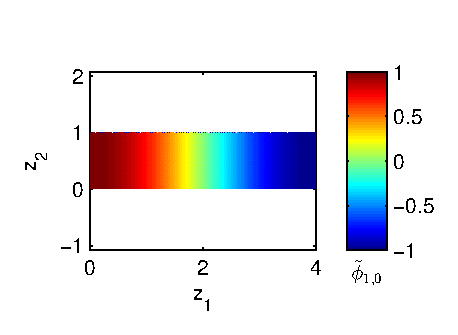
\includegraphics[width=\textwidth]{ch-harmonics/figures/strip_cnts1}
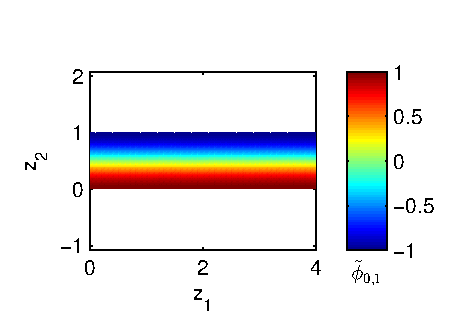
\includegraphics[width=\textwidth]{ch-harmonics/figures/strip_cnts2}
\caption{}
\label{subfig:strip_efuncs}
\end{subfigure}
%
\begin{subfigure}{0.3\textwidth}
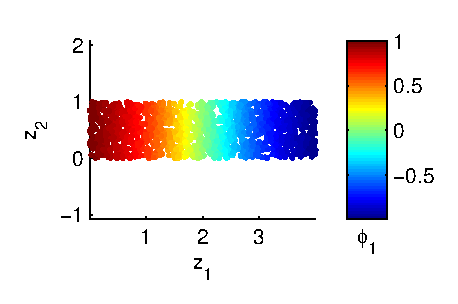
\includegraphics[width=\textwidth]{ch-harmonics/figures/strip_discrete1}
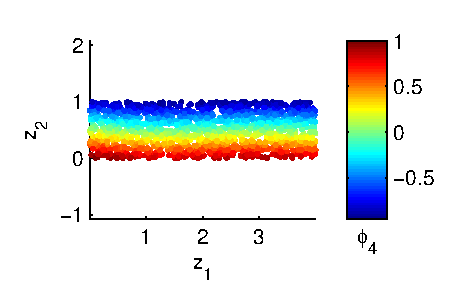
\includegraphics[width=\textwidth]{ch-harmonics/figures/strip_discrete4}
\caption{}
\label{subfig:strip_evecs_uniform}
\end{subfigure}
%
\begin{subfigure}{0.3\textwidth}
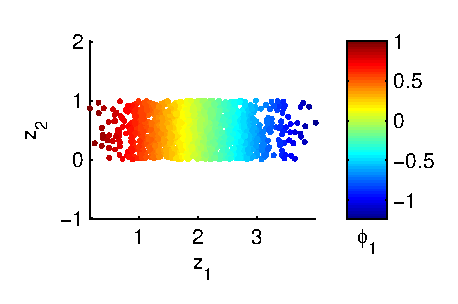
\includegraphics[width=\textwidth]{ch-harmonics/figures/strip_nonuniform1}
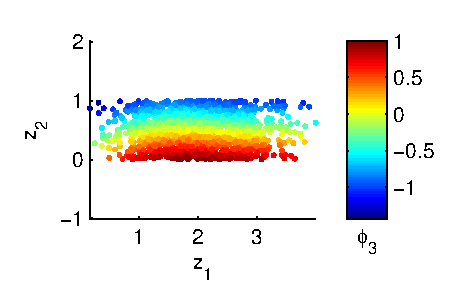
\includegraphics[width=\textwidth]{ch-harmonics/figures/strip_nonuniform2}
\caption{}
\label{subfig:strip_evecs_nonuniform}
\end{subfigure}
%
\caption[Eigenfunctions of the Laplace-Beltrami operator on a two-dimensional strip]{(a) Two-dimensional continuous strip colored by the eigenfunctions $\tilde{\phi}_{1, 0} = \cos \left( {\pi z_1}/{L_1} \right)$, and $\tilde{\phi}_{0, 1} = \cos \left( {\pi z_2}/{L_2} \right)$. (b) Two-dimensional strip with uniform sampling colored by the first and fourth (non-trivial) eigenvectors of the discrete Laplacian. (c) Two-dimensional strip with data sampled from a Gaussian distribution in $z_1$ and sampled uniformly in $z_2$, colored by the first and third (non-trivial) eigenvectors of the discrete Laplacian. Note that in all cases we uncover parameterizations which are one-to-one with $z_1$ and $z_2$.}
\end{figure}

In recent years, it has been noted that the eigenfunctions of the \emph{continuous} Laplace-Beltrami operator provide ``good" coordinates for a manifold \cite{jones2008}.
%
Thus, we start by considering a continuous setting where rigorous analysis is available for specific examples.
%
%Using such an example, we will show that the existence of repeated eigendirections is inherent to the manifold learning setup based on Laplace operators, and that the identification of the unique eigendirections is nontrivial.
%%
%The existence of these challenges in the continuous setting implies that, even in the limit of infinite data, such repeated eigendirections still pose a problem for analysis.
%
To illustrate why these eigenfunctions provide appropriate coordinates, consider a two-dimensional strip with edge lengths $L_1$ and $L_2$.
%
The eigenvalues of the Laplace-Beltrami operator with Neumann boundary conditions are given by
\begin{equation} \label{eq:evals}
\tilde{\lambda}_{k_1, k_2} = \left( \frac{k_1 \pi}{L_1} \right)^2 + \left( \frac{k_2 \pi}{L_2} \right)^2
\end{equation}
for $k_1, k_2 = 0, 1, 2, \dots$,
and the corresponding eigenfunctions are
\begin{equation} \label{eq:efuncs}
\tilde{\phi}_{k_1, k_2} = \cos \left( \frac{k_1 \pi z_1}{L_1} \right) \cos \left( \frac{k_2 \pi z_2}{L_2} \right)
\end{equation}
where $z_1$ and $z_2$ denote the two coordinates of the strip \cite{singer2008non}.
%
We note that the eigenfunctions $\tilde{\phi}_{1, 0} = \cos \left( {\pi z_1}/{L_1} \right)$ and $\tilde{\phi}_{0, 1} = \cos \left( {\pi z_2}/{L_2} \right)$ are one-to-one with the $z_1$ and $z_2$ coordinates, respectively, and therefore yield a parametrization of the underlying manifold (see Figure~\ref{subfig:strip_efuncs}).
%
Furthermore, the corresponding eigenvalues $\tilde{\lambda}_{1,0}$ and $\tilde{\lambda}_{0,1}$ provide a measure of $L_1$ versus $L_2$: as the ratio between $L_1$ and $L_2$ increases, the gap between $\tilde{\lambda}_{1,0}$ and $\tilde{\lambda}_{0,1}$ also increases (this will be discussed further in Section~\ref{sec:relative_lengths}).
%
%The analytic form of the eigenfunctions in \eqref{eq:efuncs} illustrates the two issues we address in this paper.
%%
%First, $z_1$ and $z_2$ are not necessarily decoupled in subsequent eigenfunctions, and a proper parametrization of the manifold is not necessarily given by the $d$ eigenfunctions associated with the smallest $d$ eigenvalues.
%% TODO: address this in later section
%%
%Second, eigenfunctions with $k_1+k_2 \ge 2$ do not describe any additional directions along the strip; we will refer to these as ``repeated eigendirections,'' and we will refer to the eigenfunctions with $k_1+k_2 =1$ as ``unique eigendirections.''
%%
%We note that, although the eigenfunctions can only be written analytically for very special cases, it has been observed empirically that the eigenfunctions often provide appropriate coordinates to parameterize more complex, nonlinear manifolds.
%%
%In addition, this problem of repeated eigendirections arises for more complex manifolds with more than two variables.


\subsection{Discrete approximation of the Laplace-Beltrami operator: diffusion maps} \label{sec:dmaps}

In most applications, we are not given a description of the continuous manifold.
%
Instead, we are given data {\em sampled} from the underlying manifold, and the parametrization of the manifold needs to be uncovered from the data.
%
It was shown in \cite{coifman2006geometric} that, in the limit of infinite data, this discrete Laplacian matrix constructed from data converges pointwise to the continuous Laplace-Beltrami operator on the manifold.
%
As a result, the eigenvectors of the discrete Laplacian approximate the eigenfunctions of this continuous operator.

Given observations $\data(1), \dots, \data(m) \in \manifold$, we first construct the weight matrix $\mathbf{W} \in \mathbb{R}^{\ndata \times \ndata}$, with
\begin{equation} \label{eq:W}
\mathbf{W}_{ij} = \exp \left( -\frac{\|\data(i) - \data(j) \|^2}{\dmeps^2} \right), \ i,j=1,\ldots,\ndata,
\end{equation}
where $\| \cdot \|$ denotes the appropriate norm for the observations, and $\dmeps$ is a characteristic distance between the observations.
%
Note that $\dmeps$ induces a notion of locality: if $\|\data(i) - \data(j) \| \gg \dmeps$, then $\mathbf{W}_{ij}$ is negligible.
%
Therefore, we only need our metric to be informative within a ball of radius $\dmeps$.
%
Points less than $\dmeps$ apart are thus considered ``close'' and points farther than $\dmeps$ apart are considered ``far away''.
%
The kernel's scale $\dmeps$ can be chosen using several heuristics \cite{rohrdanz2011determination, coifman2008graph}; we often take $\dmeps$ to be the median of the pairwise distances between the data points.
%
We then construct the diagonal matrix $\mathbf{D} \in \mathbb{R}^{\ndata \times \ndata}$, with $\mathbf{D}_{ii} = \sum_j \mathbf{W}_{ij}$, and form the matrix $\widetilde{\mathbf{W}} = \mathbf{D}^{-\alpha} \mathbf{W} \mathbf{D}^{-\alpha}$, where $0 < \alpha < 1$.
%
Next, we construct the diagonal matrix $\widetilde{\mathbf{D}} \in \mathbb{R}^{m \times m}$, with $\widetilde{\mathbf{D}}_{ii} = \sum_j \widetilde{\mathbf{W}}_{ij}$, and the matrix $\mathbf{A}  = \widetilde{\mathbf{D}}^{-1} \widetilde{\mathbf{W}}.$

If the data $\data(1), \dots, \data(m)$ are sampled from $\manifold$ with some density $q$, then, for $\dmeps \rightarrow 0$ and $\ndata \rightarrow \infty$ (with the appropriate rates), the discrete matrix converges to the following continuous limit operators with Neumann boundary conditions \cite{coifman2006geometric}
\begin{equation} \label{eq:limiting_operator}
\begin{aligned}
\frac{1}{\dmeps^2}(\mathbf{I}-\mathbf{A}) \phi &\rightarrow \nabla^2 \phi - 2\nabla U \cdot \nabla \phi, &&\alpha = 0 \\
\frac{1}{\dmeps^2}(\mathbf{I}-\mathbf{A}) \phi &\rightarrow \nabla^2 \phi - \nabla U \cdot \nabla \phi, &&\alpha = 1/2 \\
\frac{1}{\dmeps^2}(\mathbf{I}-\mathbf{A}) \phi &\rightarrow \nabla^2 \phi, &&\alpha = 1
\end{aligned}
\end{equation}
where $U = - \log q$.
%
The different limit operators, depending on the choice of $\alpha$, imply that nonuniform sampling on the manifold may have different effects.
%
In subsequent chapters, we will use the $\alpha=0$ embedding unless otherwise noted.
%
Note that by setting $\alpha=1$, one can factor out the density effects in the weight matrix, and the discrete Laplacian matrix approaches the Laplace-Beltrami operator on the manifold $\manifold$.
%
The eigenvectors $\phi_0, \phi_1, \dots, \phi_{\ndata-1}$ of $\mathbf{A}$ approximate the eigenfunctions of the Laplace-Beltrami operator on $\manifold$,
and the eigenvalues $\lambda_0, \lambda_1, \dots, \lambda_{\ndata-1}$ of $\mathbf{A}$ are related to the eigenvalues of the continuous operator by
\begin{equation} \label{eq:evals_relationship}
\lambda_k = \exp \left( -\frac{\epsilon^2}{4} \tilde{\lambda}_{k_1, k_2}  \right).
\end{equation}
%
As discussed previously, the eigenfunctions provide a parametrization of the manifold, such that $\phi_{j}(i)$ yields the $j^{th}$ embedding coordinate for $\data(i)$.
%
The standard diffusion maps embedding incorporates eigenvalue weights \cite{coifman2005geometric, coifman2006geometric},
%
\begin{equation} \label{eq:dmaps_embed_full}
\data(i) \mapsto
\begin{pmatrix}
\lambda_1^\tau \phi_1(i) \\
\lambda_2^\tau \phi_2(i) \\
\vdots \\
\lambda_{\ndata-1}^\tau  \phi_{\ndata-1}(i)
\end{pmatrix}
\end{equation}
%
where we order the eigenvectors such that $|\lambda_0| \ge |\lambda_1| \ge \dots \ge |\lambda_{m-1}|$, and $\tau \ge 0$ is a parameter (in our examples, we will take $\tau=0$, which corresponds to the Laplacian Eigenmaps formulation).
%
Because the matrix $\mathbf{A}$ is row-stochastic ($\sum_j \mathbf{A}_{ij} = 1$),  $\lambda_0 = 1$ and $\phi_0$ is a trivial constant vector.
%
The distance induced by this embedding is called the standard diffusion distance,
%
\begin{equation}
D^2_\tau(z(i), z(j)) = \sum_{k=1}^{m-1} \lambda_k^{2 \tau} \left( \phi_k(i) - \phi_k(j)  \right)^2.
\end{equation}
%
The diffusion maps embedding therefore projects the data into a space where the Euclidean distance is equivalent to the diffusion distance.
%
If the eigenvalues exhibit a spectral gap, where $|\lambda_1| \ge |\lambda_2| \ge \dots \ge |\lambda_\lowdim | \gg |\lambda_{\lowdim+1} | \ge \dots \ge |\lambda_{\ndata-1}|$, then one can embed the data in the first $\lowdim$ eigenvectors,
\begin{equation} \label{eq:dmaps_embed_reduced}
\data(i) \mapsto
\begin{pmatrix}
\lambda_1^\tau \phi_1(i) \\
\lambda_2^\tau \phi_2(i) \\
\vdots \\
\lambda_{\lowdim}^\tau  \phi_{\lowdim}(i)
\end{pmatrix}
\end{equation}
%
while still approximately retaining the diffusion distance.

Figures~\ref{subfig:strip_evecs_uniform}--\ref{subfig:strip_evecs_nonuniform} shows data sampled from a strip, colored by eigenvectors of $\mathbf{A}$.
%
In cases of both uniform and nonuniform sampling, the selected eigenvectors are one-to-one with $z_1$ and $z_2$, and thus parameterize the manifold.
%
However, we briefly note that the two diffusion maps coordinates which parameterize the manifold are not guaranteed to be the first two eigenvectors.
%
This is the issue of ``repeated eigendirections,'' where some eigenvectors are higher harmonics of previous eigenvectors and do not capture any new directions in the data; we will discuss this issue in more detail in \chap~\ref{ch:harmonics}.
%
%TODO: maybe we can put here the new figures for the different values of $\alpha$ instead of these figures.
%
Although we have considered a very simple example of a two-dimensional strip for illustrative purposes, common practice is to use these tools for high-dimensional, nonlinear data sets.

%From the previous section, we know that the eigenfunctions with $(k_1, k_2) =(1, 0)$ and $(k_1, k_2) =(0, 1)$ provide embedding coordinates for the manifold; these two eigenfunctions are both uncoupled and not repeated.
%%
%From \eqref{eq:evals}, we see that sorting the eigenvectors by the magnitude of the corresponding eigenvalues implies that these two eigenvectors are guaranteed to appear before any coupled or repeated eigendirections.
%%
%However, these eigenvectors are {\em not} guaranteed to appear as the first two (non-trivial) eigenvectors, as harmonics of the first eigendirection (i.e., $\cos \left( n \pi z_1 / L_1 \right)$ with $n > 1$) could appear before the second.
%%
%We note that, in contrast to our simple illustrative example, for most data sets of interest, the coordinates for the underlying manifold are unknown and cannot easily be obtained from the coordinates of the original data, and identifying which eigenvectors correspond to unique eigendirections is nontrivial.




%\section{Diffusion maps} \label{sec:dmaps}
%
%Diffusion maps is an unsupervised, nonlinear data mining algorithm.
%%
%Given $\ndata$ data points $\data(1), \dots, \data(\ndata)$ (typically vectors in a high-dimensional vector space) which lie on a lower-dimensional manifold $\manifold$, the aim of diffusion maps is to uncover a parametrization $f(\data)$ of the data which captures the notion of locality with respect to the manifold: points that are ``close" in the original space should also be ``close" in the coordinates $f$.
%%
%%From pairwise distances, we want to extract a {\em global} parametrization of the data that represents the slow variables.
%%
%%We will use diffusion maps \cite{Coifman2006, coifman2005geometric}, a kernel-based manifold learning technique, to extract a global parametrization using the local distances.
%%
%We first construct the kernel matrix $\mathbf{W} \in \mathbb{R}^{\ndata \times \ndata}$, where
%\begin{equation} \label{eq:dmaps_kernel}
%\mathbf{W}_{ij} = \exp \left( -\frac{\|\data(i) - \data(j) \|^2}{\dmeps^2} \right).
%\end{equation}
%Here, $\| \cdot \|$ denotes the appropriate norm, and $\dmeps$ is the kernel scale
%and denotes a characteristic distance within the data set.
%%
%Note that $\dmeps$ induces a notion of locality: if $\|\data(i) - \data(j) \| \gg \dmeps$, then $\mathbf{W}_{ij}$ is negligible.
%%
%Therefore, we only need our metric to be informative within a ball of radius $\dmeps$.
%%
%Points less than $\dmeps$ apart are thus considered ``close'' and points farther than $\dmeps$ apart are considered ``far away''.
%%
%$\dmeps$ can be chosen using several techniques (see, for example \citep{coifman2008graph, rohrdanz2011determination});
%we often use the median of the pairwise distances as $\dmeps$, as it empirically often yields good results (since each data point is connected to approximately half of the other data points).
%
%%We note that the eigenvectors $\phi_0, \dots, \phi_{\ndata-1}$ solve the following optimization problem \citep{Belkin2003}
%We then consider solving the following optimization problem \citep{Belkin2003}
%\begin{equation} \label{eq:dmaps_opt_problem}
%\argmin_{f} \sum_{ij} \mathbf{W}_{ij} (f(\data(i)) - f(\data(j)))^2.
%\end{equation}
%%
%Because of our definition of the matrix $\mathbf{W}$, solving this optimization problem will preserve local geometry, such that $f(\data(i))$ and $f(\data(j))$ will be similar if $\data(i)$ and $\data(j)$ are close.
%%
%To solve \eqref{eq:dmaps_opt_problem}, we construct the diagonal matrix $\mathbf{D} \in \mathbb{R}^{\ndata \times \ndata}$, with
%\begin{equation}
%\mathbf{D}_{ii} = \sum_{j=1}^\ndata W_{ij}.
%\end{equation}
%%
%We compute the eigenvalues $\lambda_0, \dots, \lambda_{\ndata-1}$ and eigenvectors $\phi_0, \dots, \phi_{\ndata-1}$ of the matrix $\mathbf{A} = \mathbf{D}^{-1}\mathbf{W}$, and order them such that $1 = \lambda_0 \ge |\lambda_1| \ge \dots \ge |\lambda_{\ndata-1}|$.
%%
%The eigenvectors are then solutions to \eqref{eq:dmaps_opt_problem}, such that each subsequent eigenvector is a solution which is orthogonal to the previous eigenvector solutions.
%%
%Because the matrix $\mathbf{A}$ is row-stochastic, the first eigenvector will always be the trivial eigenvector $\phi_0 = \begin{bmatrix} 1 & 1 & \cdots & 1 \end{bmatrix}^T$ (which corresponds to a trivial solution to \eqref{eq:dmaps_opt_problem}).
%%
%The next few eigenvectors provide embedding coordinates for the data, so that $\phi_j(i)$, the $i^{th}$ entry of $\phi_j$, provides the $j^{th}$ embedding coordinate for $\data(i)$ (modulo higher harmonics which characterize
%the same direction in the data; see \cite{ferguson2010systematic} and \chap~\ref{ch:harmonics}).
%%
%The mapping
%\begin{equation} \label{eq:dmaps_embed_full}
%\data(i) \mapsto
%\begin{pmatrix}
%\lambda_1^\tau \phi_1(i) \\
%\lambda_2^\tau \phi_2(i) \\
%\vdots \\
%\lambda_{\ndata-1}^\tau  \phi_{\ndata-1}(i)
%\end{pmatrix}
%\end{equation}
%is the diffusion maps embedding for the data, where $\tau > 0$ is a parameter.
%%
%We typically take $\tau=0$ in our analysis, which corresponds to the Laplacian Eigenmaps embedding \cite{Belkin2003}.
%%
%We then define the diffusion distance $D_\tau (\data(i), \data(j))$ as
%\begin{equation}
%D_\tau^2 (\data(i), \data(j)) = \sum_{k=1}^{\ndata-1} \lambda_k^{2\tau} \left( \phi_k(i)- \phi_k(j) \right)^2.
%\end{equation}
%%
%The diffusion maps embedding therefore projects the data into a space where the Euclidean distance is equivalent to the diffusion distance.
%%
%If the eigenvalues exhibit a spectral gap, where $|\lambda_1| \ge |\lambda_2| \ge \dots \ge |\lambda_\lowdim | \gg |\lambda_{\lowdim+1} | \ge \dots \ge |\lambda_{\ndata-1}|$, then one can embed the data in the first $\lowdim$ eigenvectors,
%\begin{equation} \label{eq:dmaps_embed_reduced}
%\data(i) \mapsto
%\begin{pmatrix}
%\lambda_1^\tau \phi_1(i) \\
%\lambda_2^\tau \phi_2(i) \\
%\vdots \\
%\lambda_{\lowdim}^\tau  \phi_{\lowdim}(i)
%\end{pmatrix}
%\end{equation}
%%
%while still approximately retaining the diffusion distance.
%%
%A more detailed discussion of the diffusion maps theory will be presented in \chap~\ref{ch:harmonics}.
%
%%This is analogous to how the eigenfunctions $\cos x$ and $\cos 2x$ of the usual Laplacian in one spatial dimension and with no flux boundary conditions are one-to-one with the values of $x$ for $0 \le x \le 1$;
%%one must check for correlations between the eigenvectors before selecting those that describe the underlying manifold geometry.




Modulo higher harmonics which characterize the same direction in the data
%(see \cite{ferguson2010systematic} and \chap~\ref{ch:harmonics})
, each retained eigenvector then parameterizes a variable for the data set of interest.
%
We note that the eigenvectors can be determined up to a scaling factor.
%
For some applications, the magnitude and/or sign of the eigenvectors are important.
%
For the work presented in \chap~\ref{ch:merging}, we must normalize the eigenvectors from different data sets so that the resulting embeddings are consistent.
%
We first scale the eigenvectors so that $\|\phi_i\| = \ndata$ (where $\ndata$ is the number of data points)
to make the embedding coordinates invariant to the size of the data set.
%twice as many samples as another data set, but with the same underlying geometry, should have twice the norm.
%
Still, the computed embedding eigenvectors, even for two identical data sets, may differ by a sign.
%
Reconciling the signs for the embeddings of different data sets can be rationally done in several ways and is somewhat problem-specific.
%
For example, if the mean of the embedding is sufficiently far from 0, we can require $\langle \phi_i \rangle > 0$;
alternatively, if there is a common region sampled by two data sets obtained from the same system, the sign of each eigenvector can be chosen to optimize the consistency of the embeddings of the common region data.
%
%We will return to the issue of embedding consistency for different data sets in our concluding discussion; for the moment, we will assume that our different sets sample the same region of data space in a representative enough way such that the correspondence between the sequences of retained eigenvectors for different embeddings is obvious.
%
Similarly, for the examples in \chap~\ref{ch:drosophila}, the sign of the eigenvector is important and is determined after analysis using {\em a priori} knowledge of the system dynamics.



%
%\subsection{Family of operators} \label{sec:diff_limit}
%
%In the limit $\dmeps \rightarrow 0$ and $\ndata \rightarrow \infty$ (with the appropriate rates), the matrix $\frac{1}{\dmeps^2} \left( \mathbf{I} - \mathbf{A} \right) $ converges to the continuous backward Fokker-Planck operator \cite{nadler2006diffusion}
%\begin{equation}
%	\mathcal{L} = \Delta - 2 \nabla U \cdot \nabla.
%	\label{eq:limiting_operator}
%\end{equation}
%where the data $\data_1, \dots , \data_\ndata$ are sampled from $\manifold$ with density proportional to $e^{-U}$.
%%
%However, we can construct a family of diffusion operators
%\begin{equation} \label{eq:kernel2}
%\mathbf{A}^{(\alpha)} = {\mathbf{D}^{(\alpha)}}^{-1} \mathbf{W}^{(\alpha)}
%\end{equation}
%for $0 \le \alpha \le 1$, where $\mathbf{W}^{(\alpha)} = \mathbf{D}^{-\alpha} \mathbf{W} \mathbf{D}^{-\alpha}$
%and $\mathbf{D}^{(\alpha)}$ is a diagonal matrix with $\mathbf{D}^{(\alpha)}_{ii} = \sum_{j=1}^\ndata \mathbf{W}^{(\alpha)}$.
%%
%We then have \cite{coifman2005geometric}
%\begin{equation}
%\begin{aligned}
%\frac{1}{\dmeps^2} \left( \mathbf{I} - \mathbf{A}^{(0)} \right) & \rightarrow \Delta - 2 \nabla U \cdot \nabla \\
%\frac{1}{\dmeps^2} \left( \mathbf{I} - \mathbf{A}^{(1/2)} \right) & \rightarrow \Delta - \nabla U \cdot \nabla \\
%\frac{1}{\dmeps^2} \left( \mathbf{I} - \mathbf{A}^{(1)} \right) & \rightarrow \Delta
%\end{aligned}
%\end{equation}
%%
%Therefore, choosing different values of $\alpha$ results in different kernel normalizations which can remove sampling density effects along the manifold.


\section{The Mahalanobis Distance}
\label{sec:mahalanobis}

The essential component of manifold learning algorithms (such as diffusion maps) is having an informative distance metric between data points, as one of the key assumptions is that points which have a small distance are close on the manifold.
%
However, often the Euclidean distance is not meaningful or informative, and we require a more sophisticated metric.
%
Here, we will discuss the Mahalanobis distance \cite{mahalanobis1936generalized}, a metric which has some nice properties that will allow us to analyze data from multiscale stochastic systems in \chap~\ref{ch:multiscale} and data from chemical simulations in \chap~\ref{ch:merging}.

Let $\mathbf{C}(t)$ be the covariance matrix associated with the measured sample $\data(t)$ (the specifics will be discussed in subsequent chapters).
%
We define a Riemannian metric between a pair of samples using the associated covariance matrices as
\begin{equation}
	d^2(\data(i), \data(j)) = 2 (\data(i) - \data(j))^T(\widehat{\mathbf{C}}(i) + \widehat{\mathbf{C}}(j))^{\dagger}(\data(i) - \data(j));
	\label{eq:mahalanobis1}
\end{equation}
this is the Mahalanobis distance (and $^{\dagger}$ denotes a pseudoinverse, since $\widehat{\mathbf{C}}$ is most likely rank-deficient).
%
The covariance matrices convey the local variability of the measurements and are utilized to explore and learn the tangent planes of the observable manifold.
%
This information is then utilized in \eqref{eq:mahalanobis1} to compare a pair of points according to the directions of their respective tangent planes.
%
%The Mahalanobis distance is invariant under affine transformations.
%%
%We assume
%\begin{equation}
%	\data(t) = \measfn(\mathbf{x}(t)),
%\end{equation}
%where the observation function $\measfn$ is bi-Lipschitz and smooth, and
%assuming the dynamics of the diffusion process in each of its underlying variables are described by normalized stochastic differential equations as
%\begin{equation}
%	d x_i(t) = a_i (\mathbf{x}(t)) dt + d W_i(t), \ i=1,\ldots,\lowdim,
%	\label{eq:dynamics}
%\end{equation}
%where $a_i$ are unknown drift functions and $\dot{W}_i(t)$ are independent white noises.
%%
%Then, by using local linearization of the function, i.e., $\data(t) = \mathbf{J}(t) \mathbf{x}(t) + \boldsymbol{\epsilon}(t)$ where $\mathbf{J}(t)$ is the Jacobian of $\measfn(\mathbf{x}(t))$ and $\boldsymbol{\epsilon}(t)$ is the residual consisting of higher-order terms, it was shown by Singer and Coifman \cite{singer2008non} that $\mathbf{C}(t) = \mathbf{J}(t)\mathbf{J}^T(t)$ and that the Mahalanobis distance approximates the Euclidean distance between the corresponding samples of the underlying process to second order, i.e.,
%\begin{equation}
%	\| \mathbf{x}(i) - \mathbf{x}(j) \|^2 = d^2(\data(i), \data(j)) + \mathcal{O}(\| \data(i) - \data(j)\|^4).
%\end{equation}
%%
%This result implies that the Mahalanobis distance is invariant to the measurement function $\measfn$, and hence,
%it yields the same distances between samples obtained under different observation functions or even partial observations.
%%
%We would like to note that, in general, $\measfn$ being bi-Lipschitz implies that $\measfn$ is invertible (on the $d$-dimensional
%manifold $\manifold$).
%%
%However, in practice, determining whether $\measfn$ contains sufficient information and is ``rich enough'' to completely determine the underlying process is a non-trivial task.
%%
%In this work, we exploit the fact that $\mathbf{C}(t) = \mathbf{J}(t)\mathbf{J}^T(t)$, which implies that $\mathbf{C}(t)$ is an $\highdim \times \highdim$ positive semidefinite matrix of rank $d$, to empirically infer the dimension $\lowdim$.
%%
%According to the spectrum of the local covariance matrices and their corresponding spectral gaps, we approximate the rank of the matrices.
%%
%Consistent rank estimates among these local covariance matrices are taken to imply that the measurements are ``rich enough", and hence, may be good indicators for the dimension $\lowdim$.
%%
%Since the dimension $\lowdim$ of the underlying process is typically considerably smaller than the dimension of the measured process $\highdim$,
%the covariance matrix is singular and non-invertible;
%%
%thus, we use the pseudo-inverse in \eqref{eq:mahalanobis1}.

In practice, for a dynamical system, the covariance matrix can be estimated from a short trajectory of samples in time around the sample $\data(t)$ by
\begin{equation} \label{eq:cov1}
	\widehat{\mathbf{C}}(t) = \sum \limits _{\tau = t-L}^{t+L} (\data(\tau) - \widehat{\boldsymbol{\mu}}(t))(\data(\tau) - \widehat{\boldsymbol{\mu}}(t))^T,
\end{equation}
where $\widehat{\boldsymbol{\mu}}(t)$ is the empirical mean of the short trajectory of samples around time $t$ and $L$ is the size of the trajectory window.
%
Alternatively, we can estimate the local covariance by using small bursts of simulation
\begin{multline} \label{eq:cov2}
\hat{\mathbf{C}}_{ij}(\data(t), \delta t)
= \\
\frac{1}{ \delta t} \left( \mathbb{E} \left[ \dataone_i (t+\delta t) \dataone_j (t+ \delta t) \mid \data(t) \right]
- \mathbb{E} \left[ \dataone_i (t+\delta t) \mid \data(t) \right] \mathbb{E} \left[ \dataone_j (t+\delta t) \mid \data(t) \right] \right) ,
\end{multline}
%
where $\delta t > 0$ is the length of the simulation burst.
%
%The Mahalanobis distance can also reduce the effects of fast variables, as will be discussed in \chap~\ref{ch:multiscale}.

%\begin{table}[tb]
%\caption{Nonlinear Intrinsic Variables Construction Algorithm}
%\hrule
%\begin{enumerate}
%
%\item
%Obtain a sequence of high-dimensional observation samples $\data(t)$.
%
%\item
%Compute the empirical covariance matrix $\widehat{\mathbf{C}}(t)$ of each sample $\data(t)$ {\em in a short window in time} according to \eqref{eq:cov1} or \eqref{eq:cov2}.
%
%\item
%Using the samples and their associated covariance matrices, compute the Mahalanobis distance between the observations \eqref{eq:mahalanobis1} .
%
%\item
%Build the pairwise affinity matrix $\mathbf{W}$ and the corresponding normalized kernel $\mathbf{W}^{(\alpha)}$ in \eqref{eq:kernel2}.
%
%\item
%Apply eigenvalue decomposition to the normalized kernel and view the values of its principal eigenvectors (modulo the possibility of
% ``higher harmonics", see text) as the Nonlinear Intrinsic Variables (NIV) of the given observations.
%
%\end{enumerate}
%\hrule
%\label{algo}
%\end{table}


\section{Angular Synchronization } \label{sec:ang_synch}

{\em This section is published in the supplemental information of \cite{dsilva2015temporal}}

As will be discussed in \chap~\ref{ch:multiscale} and \chap~\ref{ch:merging}, the Mahalanobis distance is useful for analyzing data which have been obscured by large noise and/or a measurement function.
%
Another source of variability that one would often like to remove is due to symmetries, when data (such as images) are collected in many different orientations.
%
When these orientational differences are a result of the experimental or imaging setup, they must be removed for informative analysis.
%
We will discuss two algorithms for registering images with respect to rotational symmetries.
%
Angular synchronization \cite{singer2011angular} is an algorithm for registering a data set given pairwise alignment information.
%
Vector diffusion maps \cite{singer2012vector} combines angular synchronization and diffusion maps to both register and uncover structure in a data set in a single computation.
%
We demonstrate these two algorithms using a synthetic data set whose relatively simple dynamics allow us to easily visualize and illustrate the main features of the different algorithms.
%
Motivated by the geometry of the {\em Drosophila} embryo images in \chap~\ref{ch:drosophila}, we construct a sequence of concentration profiles defined on a ring, and rotate each ring randomly around its center; an example is shown in \fig~\ref{fig:1d_demo}A.
%
Rotation of the ring corresponds to shifting (with periodic boundary conditions) the one-dimensional concentration profile shown at the bottom of \fig~\ref{fig:1d_demo}A (the symmetry group is $SO(2)$, the group of all two-dimensional proper rotations).
%
Each concentration profile is a noisy Gaussian (shown in \fig~\ref{fig:1d_demo}B), and the Gaussians increase in intensity as a function of ``time".
%
We discretize the profiles into $100$ points, so our numerical data will be $100$-dimensional vectors (the corresponding symmetry group for the discretized profiles is $\mathbb{Z}_{100}$, the group of integers modulo $100$).
%
\fig~\ref{fig:1d_demo}C shows the entire data set; the concentration profiles have been stacked in an array, so that each row corresponds to a single profile.
%
Because the profiles are unregistered and unordered, the underlying dynamics (a Gaussian whose amplitude grows in time) are not readily apparent.

\begin{figure}
\centering
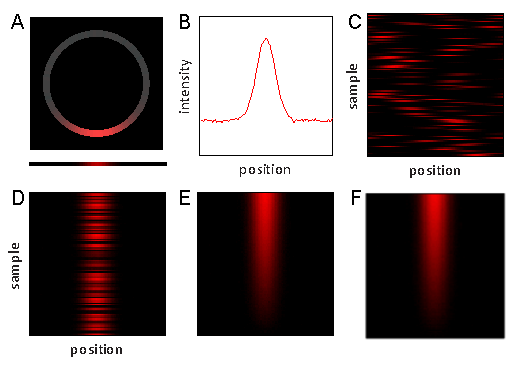
\includegraphics[width=0.7\textwidth]{ch-drosophila/figures/figS2}
\caption[Synthetic data set used to illustrate registration and ordering algorithms]{Synthetic data set used to illustrate the data processing algorithms. (A) One-dimensional concentration profile on a ring (top), and the corresponding profile on a line (bottom). (B) Intensity corresponding to the profile in A. (C) An ensemble of concentration profiles, each of the form described in A. Each row in the array corresponds to a single profile. {(D)} The profiles in {C}, now registered using angular synchronization. {(E)} The profiles in {D}, now temporally ordered using diffusion maps.  {(F)} The profiles in {C}, registered and temporally ordered in a single step using vector diffusion maps.}
\label{fig:1d_demo}
%\customlabel{subfig:1d_example}{\ref{fig:1d_demo}{\it A}}
%\customlabel{subfig:1d_intensity}{\ref{fig:1d_demo}{\it B}}
%\customlabel{subfig:1d_unaligned_unordered}{\ref{fig:1d_demo}{\it C}}
%\customlabel{subfig:1d_aligned_unordered}{\ref{fig:1d_demo}{\it D}}
%\customlabel{subfig:1d_aligned_ordered}{\ref{fig:1d_demo}{\it E}}
%\customlabel{subfig:1d_aligned_ordered_vdm}{\ref{fig:1d_demo}{\it F}}
\end{figure}

The angular synchronization algorithm aligns pairs of data points with respect to a given symmetry group from pairs of alignment measurements \citep{singer2011angular}.
%
Let $ \data(1), \dots, \data(\ndata)$ denote the signals that we wish to align with respect to rotations;
each signal is a function defined on the unit circle (on the plane).
%
First assume that each signal $\data(i)$ is a {\it noisy} rotated copy of the underlying signal $\data_{true}$
(which we are {\it not} given), such that
\begin{equation}
\data(i) = f(\data_{true}, \theta_i) + \mathbf{\xi}(i)
\end{equation}
where the function $f(\data_{true}, \theta_i)$ rotates the signal $\data_{true}$ by $\theta_i$ degrees, and $\mathbf{\xi}_i$ is a (typically Gaussian) noise term.
%
Our goal is to recover $\theta_1, \dots, \theta_\ndata$.
%
Up to noise,
\begin{equation} \label{eq:pairwise_rot}
\data(i) \approx f(\data(j), \theta_i - \theta_j) ;
\end{equation}
note that \eqref{eq:pairwise_rot} does not require knowledge of $\data_{true}$.
%
We can obtain an {\it estimate} of $\theta_i - \theta_j$ by computing the rotation that optimally aligns $\data(j)$ to $\data(i)$,
i.e., %$\theta_{ij} \approx \theta_i - \theta_j$, where
%
\begin{equation} \label{eq:opt_angle}
\theta_i - \theta_j \approx \theta_{ij} = \argmin_{\theta} \|\data(i) - f(\data(j), \theta)\|^2.
\end{equation}
%
Practically, the signals are discretized in a $\highdim$-long vector (the local intensity at $n$ equidistant points around the circle);
rotating the function by an angle $\theta$ then corresponds to cyclically shifting the elements of $\data(i)$
by $\frac{\theta_i}{2 \pi} \highdim$ (rounded to the nearest integer to obtain a valid shift).
%
For the one-dimensional discretized profiles shown in \fig~\ref{fig:1d_demo}, we exhaustively search over all $\highdim=100$ possible shifts of the signals to obtain the optimal angles in \eqref{eq:opt_angle}.
%
Alternatively, for continuous signals, an optimization algorithm
can be used \citep{ahuja2007template}.

Rather than work with the angles $\theta_{ij}$ directly, it is more convenient to consider the rotation matrices,
\begin{equation} \label{eq:R_theta}
\mathbf{R}(\theta_{ij}) = \begin{bmatrix}
\cos(\theta_{ij}) & -\sin(\theta_{ij}) \\
\sin(\theta_{ij}) & \cos(\theta_{ij})
\end{bmatrix},
\end{equation}
which we can think of as operating on the points of the unit circle (on the plane) on which our signal is defined.
%
Successive rotations correspond to multiplication of the corresponding rotation matrices: $\mathbf{R}(\gamma_1 + \gamma_2) = \mathbf{R}(\gamma_1) \mathbf{R}(\gamma_2)$.
%
Due to the orthogonality of rotation matrices, $\mathbf{R}(-\gamma) = \mathbf{R}(\gamma)^T$.

Let $\rotdim$ denote the dimension of the rotation matrices we are considering (for planar rotations, $\mathbf{R}(\theta_{ij}) \in \mathbb{R}^{2 \times 2}$ and $\rotdim=2$).
%
We construct the matrix $\mathbf{H} \in \mathbb{R}^{\ndata \rotdim \times \ndata \rotdim}$, where $\mathbf{H}$ is an $m \times m$ matrix of $\rotdim \times \rotdim$ blocks, with the $i,j^{th}$ block of $\mathbf{H}$, $\mathbf{H}_{ij}$, defined as
\begin{equation} \label{eq:H_to_R}
\mathbf{H}_{ij} = \mathbf{R}(\theta_{ij}).
\end{equation}
%
%
Under our assumption that $\theta_{ij} \approx \theta_i - \theta_j$, $\mathbf{H}_{ij} \approx \mathbf{R}(\theta_i) \mathbf{R}(\theta_j)^T$
%\begin{equation}
%H_{ij} = R(\theta_{ij}) \approx R(\theta_i - \theta_j) = R(\theta_i) R(-\theta_j) = R(\theta_i) R(\theta_j)^T,
%\end{equation}
 and
\begin{equation} \label{eq:H_low_rank}
	\mathbf{H} \approx
	\begin{bmatrix}
	\mathbf{R}(\theta_1) \\
	\mathbf{R}(\theta_2) \\
	\vdots \\
	\mathbf{R}(\theta_\ndata)
	\end{bmatrix}
	\begin{bmatrix}
	\mathbf{R}(\theta_1)^T \mathbf{R}(\theta_2)^T \dots \mathbf{R}(\theta_\ndata)^T
	\end{bmatrix}.
\end{equation}
%
It follows directly from \eqref{eq:H_low_rank} that the top block eigenvector of $\mathbf{H}$ contains our best estimates of $\mathbf{R}(\theta_1), \mathbf{R}(\theta_2), \dots, \mathbf{R}(\theta_m)$.
%
Let $\phi_0, \phi_1, \dots, \phi_{\ndata \rotdim-1}$ denote the eigenvectors of $\mathbf{H}$ ordered so that $|\lambda_0| \ge |\lambda_1| \ge \dots \ge |\lambda_{\ndata \rotdim -1}|$, where $\lambda_i$ is the eigenvalue corresponding to $\phi_i$.
%
Then,
\begin{equation} \label{eq:R_hat}
\hat{\mathbf{R}} =
\begin{bmatrix}
\hat{\mathbf{R}}_1 \\
\hat{\mathbf{R}}_2 \\
\vdots \\
\hat{\mathbf{R}}_\ndata
\end{bmatrix} =
\begin{bmatrix}
| & | & & | \\
\phi_0 & \phi_1 & \dots & \phi_{\rotdim-1} \\
| & | & & |
\end{bmatrix},
\end{equation}
where $\hat{\mathbf{R}}_i \in \mathbb{R}^{\rotdim \times \rotdim}$ is (nearly) the estimate for $\mathbf{R}(\theta_i)$.
%
To obtain our estimate of $\mathbf{R}(\theta_i$), denoted $\mathbf{R}_{i, est}$, we project $\hat{\mathbf{R}}_i$ onto the closest orthogonal matrix,
\begin{equation} \label{eq:R_est}
\mathbf{R}_{i, est} = \mathbf{U}_i \mathbf{V}_i^T,
\end{equation}
where $\mathbf{U}_i$ and $\mathbf{V}_i$ are the left and right singular vectors, respectively, of $\hat{\mathbf{R}}_i$.
%
We adjust the sign of $\phi_1$ so that $det(\mathbf{R}_{i, est}) = +1$, ensuring proper rotations
(note that systematically incorporating improper rotations is also possible \citep{goemans1995improved, bandeira2013cheeger}).
%
We estimate $\theta_{i}$ by inverting \eqref{eq:R_theta}, and register the signals by rotating signal $i$ by $-\theta_i$.
%
We note that, in our actual computations, the pairwise rotations $\theta_{ij}$ are computed in a discrete setting, then the overall
synchronization is performed in the continuum context to obtain $\theta_i$, and the results are rounded to give the closest
discrete shift.

Importantly, this formulation also considers {\it higher-order} consistency information.
%
For example, given our pairwise estimates $\mathbf{R}_{ij}$, we know that relationships of the form
\begin{equation} \label{eq:triplet_consistency}
\mathbf{R}(\theta_{ik}) \mathbf{R}(\theta_{kj}) \approx \mathbf{R}(\theta_i) \mathbf{R}(\theta_k)^T \mathbf{R}(\theta_k) \mathbf{R}(\theta_j)^T = \mathbf{R}(\theta_i) \mathbf{R}(\theta_j)^T
\end{equation}
should also hold.
%
Note that
\begin{equation}
(\mathbf{H}^2)_{ij} = \sum_k \mathbf{R}(\theta_{ik}) \mathbf{R}(\theta_{kj});
\end{equation}
therefore, {\it all} information of the form in \eqref{eq:triplet_consistency} is contained in the matrix $\mathbf{H}^2$ (and higher order
consistency information in its higher powers).
%
Because $\mathbf{H}$ and $\mathbf{H}^2$ have the same eigenvectors, our problem formulation accounts for not only pairwise alignment information, but also these higher-order considerations.

\section{Vector Diffusion Maps}

Vector diffusion maps combines the algorithms of angular synchronization and diffusion maps into a single computation that both removes rotational symmetries and parameterizes the data {\em modulo} these symmetries \cite{singer2012vector}.
%
Given data points $\data(1), \dots, \data(\ndata)$, one first constructs the matrix $\mathbf{S} \in \mathbb{R}^{\ndata \rotdim \times \ndata \rotdim}$, with the $i,j^{th}$ block of $\mathbf{S}$, $\mathbf{S}_{ij}$, defined as
\begin{equation} \label{eq:vdm_S}
	\mathbf{S}_{ij} = \mathbf{A}_{ij} \mathbf{H}_{ij}
\end{equation}
%
where $\mathbf{A}_{ij} \in \mathbb{R}$ (defined in \sec~\ref{sec:dmaps}) pertains to the diffusion kernel between data points, and $\mathbf{H}_{ij} \in \mathbb{R}^{\rotdim \times \rotdim}$ (defined in \eqref{eq:H_to_R}) pertains to the pairwise alignment between data points.
%
It is important to note that distance $\| \data(i) - \data(j) \|$ used in the diffusion kernel in \eqref{eq:W} is the distance between data points {\it after} after pairwise alignment, i.e., the minimum distance between all possible shifts of the two data points.
%
In the language of symmetry groups, this distance is a metric between the orbits induced by the relevant symmetry group.

One then computes the eigenvalues $\lambda_0, \lambda_1, \dots, \lambda_{\ndata \rotdim-1}$ and eigenvectors $\phi_0, \allowbreak \phi_1, \dots, \allowbreak \phi_{\ndata \rotdim-1}$ of $\mathbf{S}$, ordered such that $|\lambda_0| \ge |\lambda_1| \ge \dots \ge |\lambda_{\ndata \rotdim-1}|$.
%
These eigenvectors contain information about {\it both} the optimal rotations (the ``synchronization" component) and the
variation of the data {\it after} the spatial symmetries have been removed.
%
Assuming that the data (after symmetries have been factored out) are relatively closely clustered, it is reasonable
to expect, as in angular synchronization, that the top (block) eigenvector of $\mathbf{S}$ contains approximations of the optimal rotations,
which can be computed in the same way from \eqref{eq:R_est}.
%
We then expect subsequent eigenvectors to contain information about the main direction(s) of data variability modulo the geometric symmetries.

In general, the embedding coordinates are given by
\begin{equation} \label{eq:vdm_coord}
\psi_{k,l} (i) = \langle \phi_k(i), \phi_l(i) \rangle,
\end{equation}
where $\phi_k(i) \in \mathbb{R}^{\rotdim}$ denotes the $i^{th}$ block of $\phi_k$,
%
If we assume that the rotations and the dynamics are uncoupled and therefore separable, then the eigenvectors of $\mathbf{S}$ have the following structure: each block eigenvector contains estimates of the optimal rotations (up to a constant rotation) multiplied by the corresponding embedding coordinate (a scalar)
%
As the first diffusion maps coordinate is constant over the data, the first block eigenvector contains only the optimal rotations.
%
The second block eigenvector (eigenvectors $\rotdim$ through $2\rotdim-1$) contains the optimal rotations, each multiplied by their second diffusion maps coordinate.
%
We can therefore recover this diffusion maps coordinate by taking inner products of the columns of the second block eigenvector with columns of the first block eigenvector.
%
The $j^{th}$ embedding coordinate will be given by $\psi_{k,l}$, where $j\rotdim  < k \le (j+1)\rotdim-1$ and $0 \le l \le \rotdim-1$,
and we select $k, l$ such that the coordinate $\psi_{k, l}$ has the largest variability, i.e., the $j^{th}$ coordinate is $\psi_{k,l}$, where $k, l$ is the solution to
\begin{equation} \label{eq:first_embed_vdm}
\max_{
\begin{matrix}
j\rotdim \le k \le (j+1)\rotdim-1 \\
0 \le l \le \rotdim-1
\end{matrix}}
 \sum_i \psi_{k,l} (i)^2.
\end{equation}

%\section{The eigenvalue spectrum}

We can use the eigenvalues from vector diffusion maps to help deduce the dimensionality of the data.
%
In diffusion maps, the largest eigenvalue will always be 1 and correspond to the trivial (constant) eigenvector, and $|\lambda_k|$ gives a measure of the importance of coordinate $\phi_k$.
%
We therefore expect to see a ``spectral gap'' in the eigenvalues which separates the meaningful coordinates from those corresponding to noise (modulo higher harmonics; see \chap~\ref{ch:harmonics} and \citep{ferguson2010systematic}).
%
In vector diffusion maps, the importance of each coordinate is measured by the product of the corresponding eigenvalues (i.e., the importance of $\psi_{k,l}$ is given by $| \lambda_k \lambda_l |$).
%
We again expect to see a ``spectral gap'' in these eigenvalue products between those corresponding to meaningful coordinates (again, modulo higher harmonics) and those corresponding to noise. 
% !TEX root = ../thesis.tex

\chapter{Reduction of Data from Multiscale Dynamical Systems \label{ch:multiscale}}

\graphicspath{{ch-multiscale/figures/}}

{\em This work was published in \citep{dsilva2015data}}

\section{Introduction}

Dynamical systems of engineering interest often contain several disparate time scales.
%
When the evolving variables are strongly coupled, resolving the
dynamics at all relevant scales can be computationally challenging and pose problems for analysis.
%
Often, the goal is to write a reduced system of equations which accurately captures the dynamics on the slow time scales.
%
These reduced models can greatly accelerate simulation efforts, and are more appropriate for integration into larger modeling frameworks.

Following the methods of Mori \cite{mori1965transport}, Zwanzig \cite{zwanzig1961memory}, and others \cite{brey1981nonlinear, chorin2000optimal, hijon2010mori}, one can reduce the number of variables needed to describe a system of differential equations.
%
However, in general, this reduction introduces memory terms.
%
It transforms a system of differential equations into a system of (lower-dimensional) {\em integro-}differential equations,
so that the reduction of the number of variables is counterpoised by the increased complexity of the  reduced model.
%
Here, we will study the special case of evolution equations which contain an inherent time scale separation;
in this case, it is possible, in principle, to obtain a reduced system of differential equations in only the slow variables {\em without memory terms}.
%
Such an analysis crucially hinges on knowing in which variables (or, more generally, functions of variables) one can write such a reduced system of slow evolution equations.

Moving averages and subsampling have often been used in simple cases as appropriate functions of variables in which to formulate slow lower-dimensional models \cite{pavliotis2007parameter}.
%
However, if the underlying dynamics are sufficiently nonlinear, such statistics may
fail to capture the relevant structures and time scales within the data (see \fig~\ref{fig:schematic_fastslow} for a schematic illustration).
%
For well-studied systems, one often has some {\em a priori} knowledge of the appropriate observables (such as phase field variables) with which to formulate the reduced dynamics \cite{chen2002phase, wheeler1992phase}.
%
However, such observables may not be immediately obvious upon inspection for new complex systems, and so we require an automated approach to construct such slow variables.

Given an explicit system of ordinary differential equations,
one can make numerical approximations, such as the quasi-steady state approximation \cite{segel1989quasi} or
the partial equilibrium approximation \cite{gallagher1986combined}, to reduce the system dimensionality without introducing memory terms.
%
There has been some recent analytical work on extending and
generalizing such ideas to more complex systems of equations \cite{ait2008closed, calderon2007fitting, contou2011model, dong2007simplification, givon2004extracting, pavliotis2007parameter,  sotiropoulos2009model}.
%
However, in many instances, closed form, analytical models are not given explicitly,
but can only be inferred from simulation and/or experimental data.
%
We therefore turn to data-driven techniques to analyze such systems and uncover the relevant dynamical modes.
%
In particular, we will use a manifold-learning based approach, as such methods can accommodate nonlinear structures in high-dimensional data.

The core of most manifold learning methods is having a notion of similarity between data points,
usually through a distance metric \cite{Belkin2003, Coifman2006, coifman2005geometric, roweis2000nonlinear, tenenbaum2000global}.
%
The distances are then integrated into a global parametrization of the data, typically through the solution of an eigenproblem.
%
In this chapter, we will analyze multiple time scale stochastic dynamical systems using data-driven methods.
%
Standard ``off-the-shelf'' manifold learning techniques which utilize the Euclidean distance are not appropriate
for analyzing data from such multiscale systems, since this metric does not account for the disparate time scales.
%
Research efforts have addressed the construction of more informative distance metrics, which are less sensitive to noise
and can better recover the true underlying structure in the data by suppressing unimportant sources of variability \cite{berry2013time, gepshtein2013image, rubner2000earth, simonyan2013fisher, xing2002distance}.
%
The Mahalanobis distance is one such metric.
%
It was shown that the Mahalanobis distance can remove the effect of {\em observing}
the underlying system variables through a complex, nonlinear function \cite{dsilva2013nonlinear, singer2008non, talmon2013empirical}.
%
Here, we will show the analogy between removing the effects of such nonlinear observation functions (in the context of data analysis), and reducing a dynamical system to remove the effects of the fast variables.
%
Our approach will build a parametrization of the data which is consistent with the underlying slow variables.
%
Because our approach is data-driven, we require no explicit description of the model, and can extract the underlying slow variables
from either simulation or experimental data.
%
Furthermore, the approach implicitly identifies the slow variables within the data and
does not require any {\em a priori} knowledge of the fast or slow variability sources.
%
Even when the underlying dynamical system is complex with nonlinear coupling between the fast and slow variables, we will show that our approach has the potential to isolate the underlying slow modes.

We will present detailed analysis for our method, and provide conditions under which it will successfully recover the slow variables.
%
Furthermore, based on this analysis, we will present data-driven protocols to tune the parameters of the method appropriately.
%
Our presentation and discussion will address two-time-scale stochastic systems; however, we claim that
our framework and analysis readily extends to systems with multiple time scale separations.
%

\begin{figure}[t]

\centering

\begin{subfigure}{0.4\textwidth}
\centering
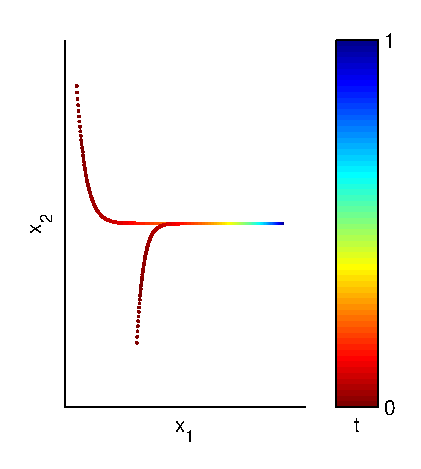
\includegraphics[width=2in]{schematic_DS1}
\caption{}
\label{subfig:schematic_fastslow1}
\end{subfigure}
%
\begin{subfigure}{0.4\textwidth}
\centering
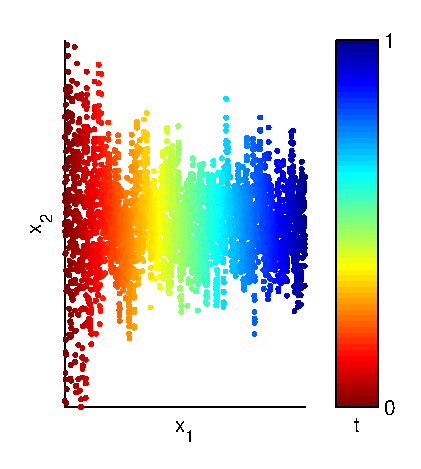
\includegraphics[width=2in]{schematic_DS2}
\caption{}
\label{subfig:schematic_fastslow2}
\end{subfigure}
%
\caption[Schematic of two-time scale data]{(\subref*{subfig:schematic_fastslow1}) Schematic of a two-dimensional, two-time scale ($\tau_1 = 50$ and $\tau_2=2$) ordinary differential equation system where the value of $x_2$ becomes slaved to the value of $x_1$.
%
In such an example, traditional data mining algorithms are sufficient to recover the slow variable. (\subref*{subfig:schematic_fastslow2}) Schematic of a two-scale two-dimensional stochastic dynamical system where {\em the statistics} of $x_2$ become slaved to $x_1$.
%
In such an example, traditional data mining algorithms will not recover the slow variable if the variance in the fast variable is too large. }
\label{fig:schematic_fastslow}
\end{figure}

\section{Multiscale Stochastic Systems} \label{subsec:multiscale_SDE}

Consider the following two-time-scale system of stochastic differential equations (SDEs),
\begin{equation} \label{eq:general_SDE}
\begin{aligned}
dx_i(t) &= a_i(\mathbf{x}(t)) dt + dW_i(t), & \: 1 \le i \le \lowdimslow \\
dx_i(t) &= \frac{a_i(\mathbf{x}(t))}{\epsilon} dt + \frac{1}{\sqrt{\epsilon}} dW_i(t) , & \: \lowdimslow+1 \le i \le \lowdim
\end{aligned}
\end{equation}
where $W_i(t)$ are independent standard Brownian motions, $$\mathbf{x}(t)  = \begin{bmatrix} x_1(t) \\ \vdots \\ x_\lowdim(t) \end{bmatrix}^T \in \mathbb{R}^\lowdim$$, and $\epsilon \ll 1$.
%
In the simple case of a linear drift function, i.e., when $a_i(\mathbf{x}(t)) = \mu _i x_i$ with $\mu_i < 0$, the probability density function of $x_i$ approaches a Gaussian with
(finite) variance $\mu_i$.
%
The time constant of the approach of the variance to equilibrium is $-1/\mu_i$ for $i=1,\ldots,\lowdimslow$ and $-\epsilon/\mu_i$ for $i=\lowdimslow+1,\ldots,\lowdim$ \cite{lelievre2013optimal}.
%
Thus, the last $\lowdim-\lowdimslow$ variables of \eqref{eq:general_SDE} rapidly approach a local equilibrium measure and exhibit fast dynamics, while the first $\lowdimslow$ variables exhibit slow dynamics.
%
A short burst of simulation will yield a cloud of points which is broadly distributed in the fast directions but narrowly distributed in the slow ones.
%
With the appropriate conditions on $a_i(\mathbf{x})$, the same can be said for more general drift
functions, where $\mu_i$ are the eigenvalues of the Jacobian of $\mathbf{a}(\mathbf{x}) = \begin{bmatrix} a_1(\mathbf{x}) & \cdots & a_\lowdim(\mathbf{x}) \end{bmatrix}^T$ \cite{villani2009hypocoercivity}.
%
Therefore, \eqref{eq:general_SDE} defines an $\lowdim$-dimensional stochastic system with $\lowdimslow$ slow
variables and $\lowdim-\lowdimslow$ fast variables, and $\epsilon$ defines the time scale separation.
%
The ratio of the powers of $\epsilon$ in the drift and diffusion terms in \eqref{eq:general_SDE} is essential,
as we require the square of the diffusivity to be of the same order as the drift as $\epsilon \rightarrow 0$ \cite{berglund2003geometric}.
%
If the diffusivity is larger, then, as $\epsilon \rightarrow 0$, the equilibrium measure will be
unbounded.
%
Conversely, if the diffusivity is smaller, the equilibrium measure will go to $0$ as $\epsilon \rightarrow 0$.

Assuming the sample average of $a_i(\mathbf{x})$ converges to a distribution which is only a function of the slow variables, then by the averaging principle \cite{freidlin2012random}, we can write a reduced SDE in {\em only} the slow variables $x_1, \dots, x_{\lowdimslow}$.
%
The aim of our work is to show how we can detect such slow variables {\em automatically} from data, in order to help inform modeling efforts and aid in the writing of such reduced stochastic models.
%
In general, we are not given the variables $\mathbf{x}(t)$ from the original SDE system, but instead, we are given some {\em observations}
 in the form $\data(t) = \measfn (\mathbf{x}(t))$.
%
We assume that $\measfn: \mathbb{R}^\lowdim \mapsto \mathbb{R}^\highdim$, $\lowdim \le \highdim$, is a deterministic (possibly nonlinear) function whose image is an $\lowdim$-dimensional manifold $\manifold$ in $\mathbb{R}^\highdim$.
%
% TODO: check whether the inverse condition is not too strong (and we only need it to apply to the domain of the samples)
%
For our analysis, we require $\mathbf{g} = \measfn ^{-1}$ to be well-defined on $\manifold$, and both $\measfn$ and $\mathbf{g}$ to be continuously differentiable to fourth order.
%
Given data $\data(t_1),\ldots,\data(t_\ndata)$ on $\manifold$ we would like to recover a parametrization of the data that is one-to-one with the
slow variables $x_1, \dots, x_\lowdimslow$.

%\section{Nonlinear Intrinsic Variables}

In order to recover the slow variables from data, we will utilize a local metric that collapses the fast directions.
%
Typically, such a metric averages out the fast variables.
%
However, simple averages are inadequate to describe data which is observed through a complicated nonlinear function.
%
Instead, we propose to use the Mahalanobis distance, which measures distances normalized by the respective variances in each local principal direction.
%
Using this metric, we still retain information about both the fast and slow directions and can
more clearly observe complex dynamic behavior within the data set.

If two points $\mathbf{x}(t_1)$ and $\mathbf{x}(t_2)$ are drawn from an $n$-dimensional
Gaussian distribution with covariance $\mathbf{C}_x$, the Mahalanobis distance between the points is defined as \cite{mahalanobis1936generalized}
\begin{equation}
	\| \mathbf{x}(t_1) - \mathbf{x}(t_2) \| _M = \sqrt{ (\mathbf{x}(t_1) - \mathbf{x}(t_2))^T \mathbf{C}_x^{-1} (\mathbf{x}(t_1) - \mathbf{x}(t_2) )  }.
\end{equation}
In particular, 
%%%YGK+CDS if $\mathbf{x}(t_1)$ and $\mathbf{x}(t_2)$ are samples 
for \eqref{eq:general_SDE}, whose covariance does not depend on $\mathbf{x}$,  $\mathbf{C}_x^{-1} = \mathrm{diag}(e_1, \ldots, e_\lowdim)$ is a constant matrix where
\begin{equation} \label{eq:e_def}
\begin{aligned}
e_i =& 1, \: & 1 \le i \le \lowdim_1 \\
e_i =& \epsilon, \: & \lowdim_1+1 \le i \le \lowdim,
\end{aligned}
\end{equation}
and the Mahalanobis distance between samples is
\begin{equation} \label{eq:rescale_x_dist}
\| \mathbf{x}(t_2) - \mathbf{x}(t_1) \|^2_M = \sum_{i=1}^\lowdim e_i \left( x_i(t_2) - x_i(t_1) \right)^2.
\end{equation}
Note that in \eqref{eq:rescale_x_dist}, the fast variables are collapsed and become $\mathcal{O}(\sqrt{\epsilon})$ small,
and so this metric is implicitly insensitive to variations in the fast variables.
%
The metric \eqref{eq:rescale_x_dist} can be rewritten as
\begin{equation} \label{eq:norm_z}
\| \mathbf{x}(t_2) - \mathbf{x}(t_1) \|^2_M = \| \mathbf{z}(t_2) - \mathbf{z}(t_1) \|^2_2
\end{equation}
where
\begin{equation} \label{eq:general_rescale}
z_i(t) = \sqrt{e_i} x_i(t).
\end{equation}
$\mathbf{z}(t)$ is a stochastic process of the same dimension as $\mathbf{x}(t)$, rescaled so that each variable has unit diffusivity.
%
This rescaling transforms our problem from one of detecting the slow variables within dynamic data to one of traditional data mining.
%
The Mahalanobis distance incorporates information about the dynamics and relevant time scales, so that using traditional data mining techniques with this metric will allow us to detect the slow variables in our data \cite{singer2009detecting}.
%
It is important to note that, in practice, we {\em never construct} $\mathbf{z}(t)$ {\em explicitly}.
%
As discussed in \cite{singer2008non}, assuming $\mathbf{f}$ is bilipschitz, the Mahalanobis distance can be extended to approximate (to fourth order) the Euclidean distance between the rescaled samples $\mathbf{z}(t)$ from accessible $\data(t) = \mathbf{f} (\mathbf{x}(t))$,
%
\begin{equation} \label{eq:mahalanobis2}
\| \data(t_2) - \data(t_1) \|^2_M = \| \mathbf{z}(t_2) - \mathbf{z}(t_1) \|^2_2 + \mathcal{O}(\| \data(t_2) - \data(t_1) \|^4_2).
\end{equation}
%
This approximation is accurate when $\| \data(t_2) - \data(t_1) \|$ is small.
%
Because we will integrate these distances into a manifold learning algorithm which only considers local distances, we can recover a parametrization of the data which is consistent with the underlying system variables $\mathbf{x}(t)$, even when the data are obscured by a function $\mathbf{f}$.
%
In \sec~\ref{sec:analysis}, we will show how we can approximate this distance directly from data $\data(t)$.

\section{Estimation of the Mahalanobis Distance} \label{sec:analysis}

\begin{figure}[t]
\centering
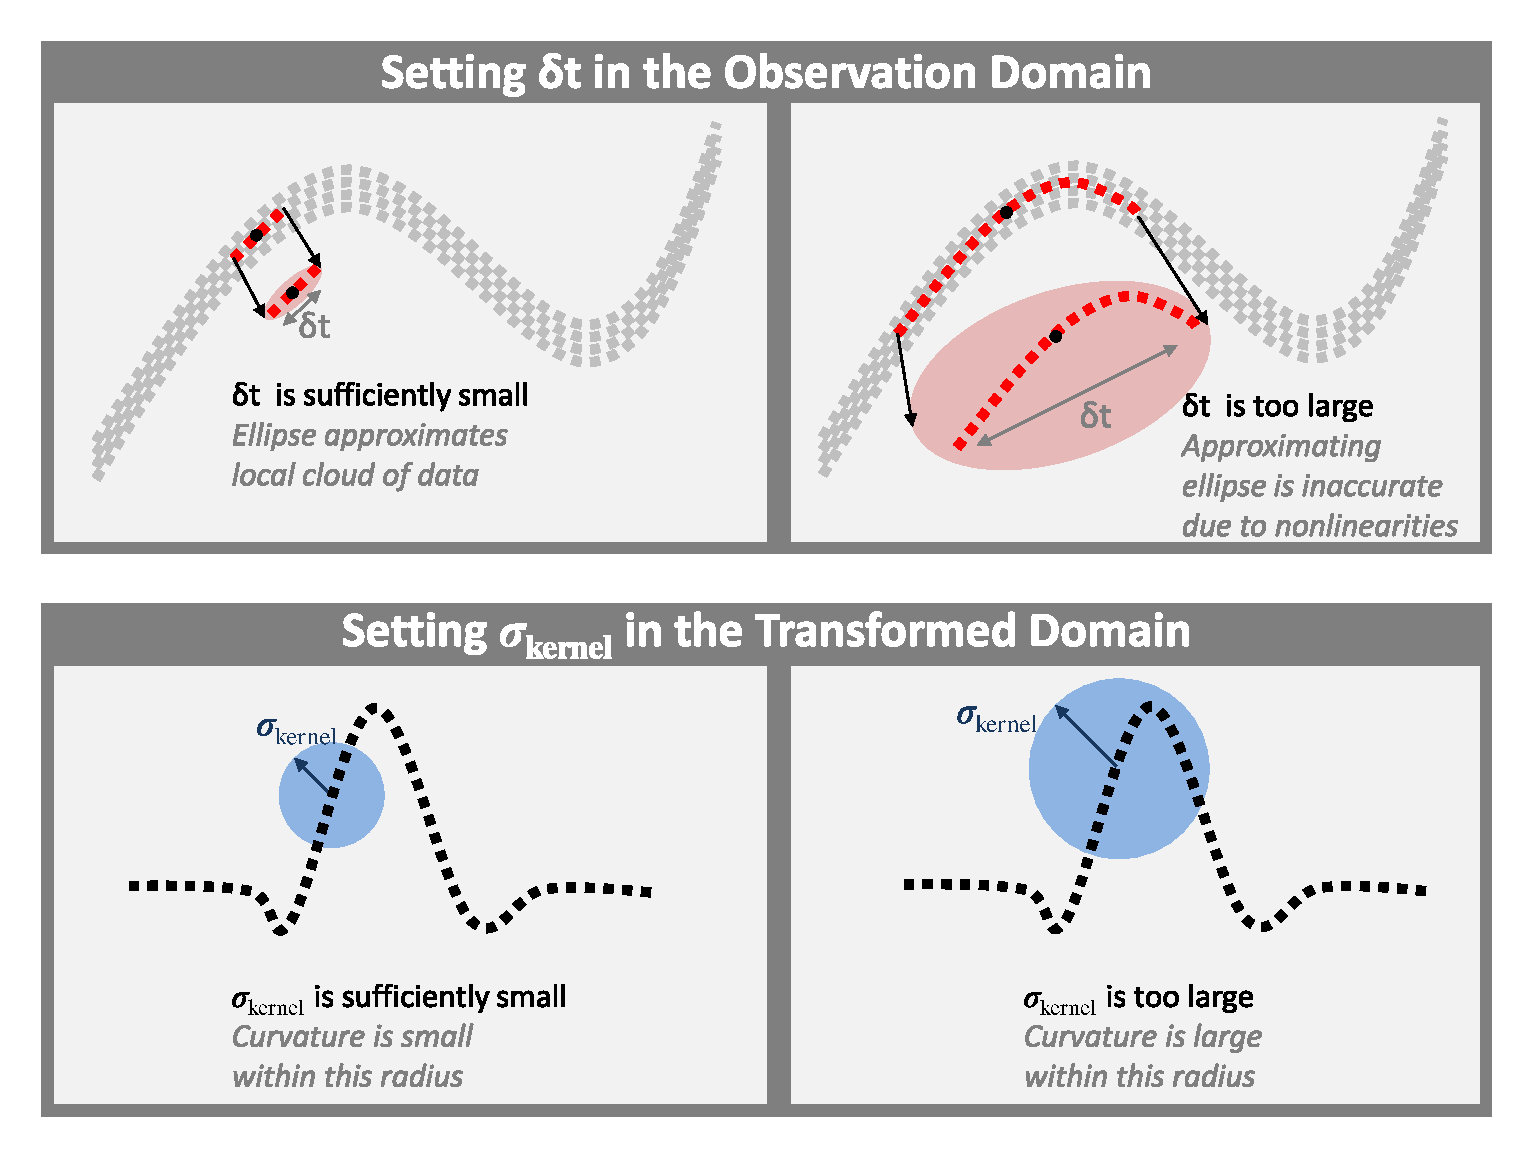
\includegraphics[width=\textwidth]{schematic}
\caption[Schematic of relevant parameters for analysis of multiscale data]{Illustration of how to choose $\delta t$ and $\dmeps$ appropriately. 	Curvature effects and other nonlinearities should be negligible within a time window $\delta t$ and within a ball of radius $\dmeps$.}
\label{fig:schematic}
\end{figure}


As previously mentioned, we do not have access to the original variables $\mathbf{x}(t)$ from the underlying original SDE system.
%
Instead, we only have measurements $\data(t) = \measfn (\mathbf{x}(t))$, and we want to estimate the Mahalanobis distance between the $\mathbf{x}$ variables from observations $\data(t)$.
%
The traditional Mahalanobis distance is defined for a fixed distribution,
whereas here we are dealing with a distribution that possibly changes as a function of position due to
nonlinearities in the observation function $\measfn$ and in the drift $\mathbf{a}(\mathbf{x})$.
%
Consequently, we use the following modified definition for the Mahalanobis distance between two points,
\begin{equation} \label{eq:mahalanobis_distance}
 \| \data(t_2) - \data(t_1) \|^2_M =
 \frac{1}{2} (\data(t_2) - \data(t_1))^T \left( \mathbf{C}^{\dagger}(\data(t_1)) + \mathbf{C}^{\dagger}(\data(t_2)) \right) (\data(t_2) - \data(t_1)),
 \end{equation}
where $\mathbf{C}(\data(t))$ is the covariance of the observed stochastic process {\em at the point} $\data(t)$,
%
and $\dagger$ denotes the Moore-Penrose pseudoinverse (since $d$ may exceed $n$).

To motivate this definition of the Mahalanobis distance, we first consider the simple linear case where $\measfn (\mathbf{x}) = \mathbf{A} \mathbf{x}$, with $\mathbf{A} \in \mathbb{R}^{\highdim \times \lowdim}$.
%
The covariance of the observed stochastic process $\measfn (\mathbf{x})$ is given by $\mathbf{C}=\mathbf{AC}_x\mathbf{A}^T$.
%
Let $\mathbf{A}= \mathbf{U} \mathbf{\Lambda} \mathbf{V}^T$ be the singular value decomposition (SVD) of $\mathbf{A}$, where $\mathbf{U} \in \mathbb{R}^{\highdim \times \lowdim}$, $\mathbf{\Lambda} \in \mathbb{R}^{\lowdim \times\lowdim}$, and $\mathbf{V} \in \mathbb{R}^{\lowdim \times \lowdim}$.
%
The pseudoinverse of the covariance matrix is $\mathbf{C}^{\dagger} = \mathbf{U} \mathbf{\Lambda}^{-1} \mathbf{V}^T \mathbf{C}_x^{-1} \mathbf{V \Lambda} ^{-1} \mathbf{U}^T$. Consequently, the Mahalanobis distance \eqref{eq:mahalanobis_distance} is reduced to
\begin{multline}
\| \data(t_2) - \data(t_1) \|^2_M \\
\begin{aligned}
&= (\data(t_2) - \data(t_1))^T  \mathbf{C}^{\dagger} (\data(t_2) - \data(t_1)) \\
 &= (\mathbf{x}(t_2) - \mathbf{x}(t_1))^T \mathbf{A}^T \mathbf{C}_x^{-1} \mathbf{A} (\mathbf{x}(t_2) - \mathbf{x}(t_1)) \\
 &= (\mathbf{x}(t_2) - \mathbf{x}(t_1))^T \mathbf{V \Lambda U}^T \mathbf{ U \Lambda}^{-1} \mathbf{V}^T \mathbf{C}_x^{-1} \mathbf{V \Lambda} ^{-1} \mathbf{U}^T \mathbf{U \Lambda V}^T (\mathbf{x}(t_2) - \mathbf{x}(t_1)) \\
 &= (\mathbf{x}(t_2) - \mathbf{x}(t_1))^T \mathbf{C}_x^{-1}  (\mathbf{x}(t_2) - \mathbf{x}(t_1)) \\
 &= \| \mathbf{x}(t_2) - \mathbf{x}(t_1) \|^2_M =  \| \mathbf{z}(t_2) - \mathbf{z}(t_1) \|^2_2 .
\end{aligned}
\end{multline}
Hence evaluating the Mahalanobis distances of the observations $\data(t) = \measfn(\mathbf{x}(t))$ using \eqref{eq:mahalanobis_distance} allows us to estimate the Euclidean distances of the rescaled variables $\mathbf{z}$ (in which the fast coordinates are collapsed).

Following \cite{singer2008non}, we will show via Taylor expansion that the Mahalanobis distance between the observations \eqref{eq:mahalanobis_distance} approximates the Euclidean
distance {\em in the rescaled variables} for general nonlinear observation functions $\measfn$ (provided $\measfn$ is bilipschitz and both $\measfn$ and $\measfn^{-1}$ are differentiable to fourth order).
%Our approximation of the pairwise distances relies on the Taylor expansion of the measurement function $\measfn$.
%
\eqref{eq:mahalanobis_distance} cannot be evaluated directly since we do not have access to the covariance matrices, so we will instead estimate the covariances directly from data.
%
We can estimate the covariance $\mathbf{C}(\data(t_0))$ empirically from a set of values $\data(t_1), \dots, \data(t_q)$ drawn from the local distribution at $\data(t_0)$.
%
One way to obtain such a set of points is to run $q$ simulations for a short time, $\delta t$, each starting from $\data(t_0)$.
%
Alternatively, we can consider a single time series of length $q \delta t$ starting from $\data(t_0)$, and then estimate the covariance
from the increments $\Delta \data(t_i) = \data(t_i) -\data(t_{i-1})$.
%
Although we will present analysis and results for the first type of estimation, the second case is often more practical in practice.
%
%It can be shown that if $q \delta t$ is sufficiently small, the errors introduced are of sufficiently low order.

Errors in our estimation of the Mahalanobis distance arise from three sources.
%
One source of error is approximating the function $\measfn$ locally as a linear function by truncating the Taylor expansion of $\measfn$ at first order.
%
An additional source of error arises from disregarding the drift in the stochastic process, and assuming that samples are drawn from a Gaussian distribution.
%
The third source comes from finite sampling effects.
%
In this work, we will address and discuss the first two sources of error (the finite sampling effects are the subject of future research).
%
We can control the effects of the errors due to truncation of the Taylor expansion by adjusting $\dmeps$; the higher-order terms in this expansion will be small for points which are close, such that adjusting $\dmeps$ will allow us to only consider distances which are
sufficiently accurate in our overall computation scheme.
%
Furthermore, we can control the errors incurred by disregarding the drift by adjusting the time scale of our simulation bursts $\delta t$.
%
Figure~\ref{fig:schematic} illustrates some of the issues in choosing the sizes $\delta t$ (or $q \delta t$ if the alternate method is used) and the parameter $\dmeps$.
%
We will present both analytical results for the error bounds, as well as an empirical methodology to set the parameters $\dmeps$ and $\delta t$ for our method to accurately recover the slow variable(s).

\subsection{Error due to the observation function $\measfn$}

We want to relate the distance in the rescaled space, $\|\mathbf{z}(t_2) - \mathbf{z}(t_1)\|_2$, to the estimated Mahalanobis distance between the observations $\| \data(t_2) - \data(t_1)\|_M$.
%
We define the error incurred by using the Mahalanobis distance to approximate the true distance as
\begin{equation}
E_M(\data(t_1), \data(t_2)) = \|\mathbf{z}(t_2) - \mathbf{z}(t_1)\|_2^2 - \| \data(t_2) - \data(t_1)\|^2_M .
\end{equation}
%
By Taylor expansion of $\mathbf{g}(y) = \measfn^{-1}(y)$ around $\data(t_1)$ and $\data(t_2)$ and averaging the two expansions, we obtain
%
\begin{equation} \label{eq:mahanaobis_error}
\begin{aligned}
& E_M\left( \data(t_1), \data(t_2) \right)
 = \\
& \begin{aligned}[t]
 \frac{1}{2} \sum_{i=1}^\lowdim \sum_{jkl=1}^{\highdim} &
\left( g_{i, (j)} (\data(t_1)) g_{i, (k,l)} (\data(t_1)) -  g_{i, (j)} (\data(t_2)) g_{i, (k,l)} (\data(t_2)) \right) \times \\
& (\dataone_j(t_2) - \dataone_j(t_1)) (\dataone_k(t_2) - \dataone_k(t_1))(\dataone_l(t_2) - \dataone_l(t_1))
\end{aligned} \\
+&
\begin{aligned}[t]
\frac{1}{8} \sum_{i=1}^\lowdim \sum_{jklm=1}^\highdim  &
\left( g_{i, (j,k)} (\data(t_1)) g_{i, (l,m)} (\data(t_1)) +  g_{i, (j,k)} (\data(t_2)) g_{i, (l,m)} (\data(t_2)) \right) \times
 \\
&(\dataone_j(t_2) - \dataone_j(t_1))  (\dataone_k(t_2) - \dataone_k(t_1))(\dataone_l(t_2) - \dataone_l(t_1)) (\dataone_m(t_2) - \dataone_m(t_1))
\end{aligned} \\
+&
\begin{aligned} [t]
\frac{1}{6} \sum_{i=1}^\lowdim \sum_{jklm=1}^\highdim &
\left( g_{i, (j)} (\data(t_1)) g_{i, (k,l,m)} (\data(t_1)) +  g_{i, (j)} (\data(t_2)) g_{i, (k,l,m)} (\data(t_2)) \right) \times \\
& (\dataone_j(t_2) - \dataone_j(t_1))  (\dataone_k(t_2) - \dataone_k(t_1))(\dataone_l(t_2) - \dataone_l(t_1))(\dataone_m(t_2) - \dataone_m(t_1))
\end{aligned} \\
+& \mathcal{O} \left(\| \data(t_2) - \data(t_1) \|^6_2 \right) ,
\end{aligned}
\end{equation}
%
where
%
\begin{equation}
\begin{aligned}
g_{i,(j)} &= \sqrt{e_i} \frac{\partial g_i}{\partial \dataone_j}
\\
g_{i,(j,k)} &= \sqrt{e_i}  \frac{\partial^2 g_i}{\partial \dataone_j \partial \dataone_k}
\\
g_{i,(j,k,l)} &= \sqrt{e_i}  \frac{\partial^3 g_i}{\partial \dataone_j \partial \dataone_k \partial \dataone_l} .
\end{aligned}
\end{equation}
%
In \cite{singer2008non}, it was shown that the error incurred by using the Mahalanobis distance to approximate the $L_2$-distance between points $\mathbf{z}(t)$ is $\mathcal{O} (\|\data_1 - \data_2 \|_2^4 )$ (see the Supplementary Materials for details).
%
We now see from \eqref{eq:mahanaobis_error} that the error is an explicit function of the second- and higher-order derivatives of $\mathbf{g} = \measfn^{-1}$ and the distance between samples $\| \data(t_2) - \data(t_1) \|_2$.
%
We would like to note that this error does not depend on the dynamics of the underlying stochastic process (as we assume the covariances at each point on the manifold are known), but is only a function of the measurement function $\measfn$.
%
The parameter $\dmeps$ in the diffusion maps calculation determines how much $E_M$ contributes to the overall analysis.
%
From \eqref{eq:W}, distances which are much greater than $\sigma_{kernel}$ are negligible in the diffusion maps computation because of the exponential kernel.
%
Therefore, we want to choose $\dmeps^2$ on the order of $\|\data(t_2) - \data(t_1)\|^2_M$ in a regime where $| E_M(\data(t_1), \data(t_2))|  \ll \|\data(t_2) - \data(t_1)\|^2_M$.
%
This is illustrated in \fig~\ref{fig:schematic}, where we want to choose $\dmeps$ small enough so that the curvature and other nonlinear effects (captured in the error term $E_M$) are negligible.
%
This will ensure that the errors in the Mahalanobis distance approximation do not greatly effect our overall analysis.

On first inspection, it would appear that our analysis indicates that $\dmeps$ should be chosen arbitrarily small.
%
However, to obtain a meaningful parametrization of the data set, there must be a nonnegligible number of data points within a ball of radius $\dmeps$ around each sample.
%
Therefore, the sampling density on the underlying manifold provides a lower bound for $\sigma_{kernel}$.

\subsection{Error due to the dynamics} \label{subsec:cov_est}

To compute the Mahalanobis distance in \eqref{eq:mahalanobis_distance}, we require $\mathbf{C}$, the covariance of the observed stochastic process $\data(t) = \measfn( \mathbf{x}(t))$.
%
We will use simulation bursts to locally explore the dynamics on the manifold of observations in order to estimate the covariance at a point $\data(t)$ from data \cite{talmon2014manifold, talmon2014intrinsic}.
%
We write the elements of the estimated covariance $\hat{\mathbf{C}}(\data(t), \delta t)$ as
%\begin{equation}
\begin{multline}\label{eq:estimated_cov_expected_value}
\hat{\mathbf{C}}_{ij}(\data(t), \delta t)
= \\
\frac{1}{\delta t} \left( \mathbb{E} \left[ \dataone_i (t+\delta t) \dataone_j (t+ \delta t) \mid \data(t) \right]
- \mathbb{E} \left[ \dataone_i (t+\delta t) \mid \data(t) \right] \mathbb{E} \left[ \dataone_j (t+\delta t) \mid \data(t) \right] \right) ,
\end{multline}
%\end{equation}
%
where $\delta t > 0$ is the length of the simulation burst.


Due to the drift in the stochastic process and the (perhaps nonlinear) measurement function $\measfn$, we incur some error by approximating the covariance at a point $\data(t)$ using simulations of length $\delta t > 0$.
%
Define the error in this approximation as
\begin{equation}
\mathbf{E}_C(\data(t), \delta t) = \hat{\mathbf{C}}(\data(t), \delta t) - \mathbf{C}(\data(t)).
\end{equation}
%
%We know that, for a stochastic process following \eqref{eq:general_SDE} and observed through a function $\measfn$, the covariance $C$ is given by
%\begin{equation} \label{eq:analytical_cov}
%C_{ij}(\data(t)) =
%\sum_{k=1}^n \frac{1}{e_k} \left. \frac{\partial f_{i}}{\partial x_k} \right|_{\mathbf{x}(t)} \left. \frac{\partial f_{j}}{\partial x_k} \right|_{\mathbf{x}(t)}
%\end{equation}
%
By It\^{o}-Taylor expansion of $\measfn$ and $\mathbf{x}(t)$ \cite{kloeden1992numerical},
%
\begin{equation} \label{eq:cov_error}
\begin{aligned}
& E_{C, ij} (\mathbf{x}(t), \delta t) = \\
 & \frac{1}{\delta t} \sum_{k=1}^\lowdim f_{i,(k)}(\mathbf{x}(t)) \mathbb{E} \left[ \int_t^{t+\delta t} \left( \int_{s_2}^{t+\delta t} f_{j,(k,0)}(\mathbf{x}(s_1)) ds_1
+ \int_t^{s_2} f_{j,(0,k)}(\mathbf{x}(s_1)) ds_1 \right) ds_2 \right] \\
&+  \frac{1}{\delta t} \sum_{k=1}^\lowdim f_{j,(k)}(\mathbf{x}(t))  \mathbb{E} \left[ \int_t^{t+\delta t} \left( \int_{s_2}^{t + \delta t} f_{i,(k,0)}(\mathbf{x}(s_1)) ds_1
+  \int_t^{s_2} f_{i,(0,k)}(\mathbf{x}(s_1)) ds_1 \right) ds_2 \right] \\
&+  \frac{1}{\delta t} \sum_{k,l=1}^\lowdim \mathbb{E} \left[ \int_t^{t+\delta t}\left( \int_t^{s_2} f_{i,(k,l)}(\mathbf{x}(s_1)) dW_{s_1, k}  \right) \left(  \int_t^{s_2} f_{j,(k,l)}(\mathbf{x}(s_1)) dW_{s_1, k} \right) ds_2 \right] \\
&+ \mathcal{O} (\delta t^{3/2})
\end{aligned}
\end{equation}
%
where
\begin{equation}
\begin{aligned}
f_{i,(k)} &= \frac{1}{\sqrt{e_k}} \frac{\partial f_i}{\partial x_k}
\\
f_{i,(k,l)} &= \frac{1}{\sqrt{e_k e_l}} \frac{\partial^2 f_i}{\partial x_k \partial x_l}
\\
f_{i,(k,0)} &= \frac{1}{\sqrt{e_k}} \sum_{l=1}^n \left( \frac{\partial}{\partial x_k} \left( \frac{a_l(\mathbf{x})}{e_l} \frac{\partial f_i}{\partial x_l} \right) + \frac{1}{2 e_l} \frac{\partial^3 f_i}{\partial x_k \partial x_l^2} \right)
\\
f_{i,(0, k)} &= \frac{1}{\sqrt{e_k}} \sum_{l=1}^n \left( \frac{a_l(\mathbf{x})}{e_l} \frac{\partial^2 f_i}{\partial x_k \partial x_l} +\frac{1}{2 e_l}  \frac{\partial^3 f_i}{\partial x_k \partial^2 x_l} \right).
\end{aligned}
\end{equation}
%
From \eqref{eq:cov_error}, the error in the covariance is $\mathcal{O}(\delta t)$ (as the $ds$ integrals are each $\mathcal{O}(\delta t)$ and the $dW$ integrals are each $\mathcal{O}(\sqrt{\delta t})$) and a function of the derivatives of the observation function $\measfn$ and the drift $\mathbf{a}$.
%
We want to set $\delta t$ such that $\|\mathbf{E}_C \| \ll \| \mathbf{C} \|$
(this is illustrated in \fig~\ref{fig:schematic}), so that the estimated covariances are accurate.
%
Note that in practice, we compute $\hat{\mathbf{C}}$ by running many simulations of length $\delta t$ starting from $\mathbf{x}(t)$, and use the sample average to approximate the expected values in \eqref{eq:estimated_cov_expected_value}.
%
We therefore incur additional error due to finite sampling; this error is ignored for the purposes of this analysis, and quantifying this error is the subject of future research.

Our analysis reveals that the errors decrease with decreasing $\delta t$; at first inspection, one would want to set $\delta t$ arbitrarily small to obtain the highest accuracy possible.
%
However, often in practice, one cannot obtain an arbitrarily refined sampling rate, such that a smaller $\delta t$ results in fewer samples with which to approximate the local covariance.%
When also accounting for these finite sampling errors, and one should take $\delta t$ as long as possible while still maintaining negligable errors from the observation function $\measfn$ and the drift $\mathbf{a}$.

\section{Illustrative Examples}

For illustrative purposes, we consider the following two-dimensional SDE
\begin{equation} \label{eq:specific_SDE}
\begin{aligned}
dx_1(t) &=& adt &+& dW_1(t)\\
dx_2(t) &=& -\frac{x_2(t)}{\epsilon} dt &+& \frac{1}{\sqrt{\epsilon}} dW_2(t)
\end{aligned}
\end{equation}
%
where $a$ is an $\mathcal{O}(1)$ constant, as a specific example of \eqref{eq:general_SDE}.
%
$x_1$ is the slow variable, and $x_2$ is a fast noise whose equilibrium measure is bounded and $\mathcal{O}(1)$.
%
\fig~\ref{fig:initial_data} shows data simulated from this SDE colored by time.
%
We would like to recover a parametrization of this data which is one-to-one with the slow variable $x_1$.

\begin{figure}[t]
\centering
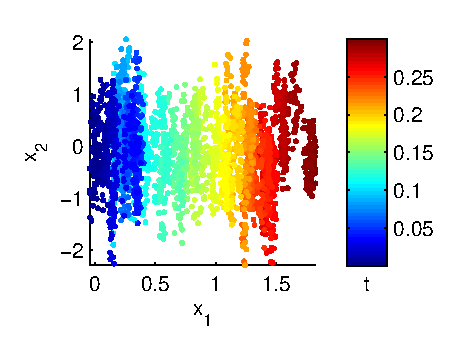
\includegraphics[width=0.5\textwidth]{data_init}
%
\caption[Linear multiscale data]{Data, simulated from \eqref{eq:specific_SDE} with $a=3$ and $\epsilon = 10^{-3}$, for $3000$ time steps with $dt = 10^{-4}$. The data are colored by time.}
\label{fig:initial_data}
\end{figure}

\subsection{Linear function} \label{subsec:linear_example}

In the first example, our observation function $\measfn$ will be the identity function,
%
\begin{equation} \label{eq:linear_transform}
\begin{aligned}
\begin{bmatrix}
y_1(t) \\ y_2(t)
\end{bmatrix} &=&
\measfn(\mathbf{x}(t)) &=&
\begin{bmatrix} x_1(t) \\ x_2(t) \end{bmatrix} \\
\mathbf{g}(\data(t)) &=& \measfn^{-1} (\data(t)) &=& \begin{bmatrix} y_1(t) \\ y_2(t) \end{bmatrix}
\end{aligned}
\end{equation}
%
where the fast and slow variables remain uncoupled.
%
In this case, there is no error incurred due to the measurement function $\measfn$ ($E_M = 0$), as the second- and higher-order derivatives of $\mathbf{g}$ are identically 0.

\subsubsection{Importance of using the Mahalanobis distance}

We want to demonstrate the utility of using the Mahalanobis distance compared to the typical Euclidean distance.
%
We compute the diffusion map embedding for the data in \fig~\ref{fig:initial_data},
using both the standard Euclidean distance and the Mahalanobis distance for the computation of the kernel in \eqref{eq:W}.
%
The data, colored by $\phi_1$ using the two different metrics, are shown in \fig~\ref{fig:NIV_versus_DMAPS}.
%
When using the standard Euclidean distance which does not account for the underlying dynamics, the first diffusion maps recovers the fast variable $x_2$, suggesting the fast modes is the dominant scale purely in terms of data analysis (\fig~\ref{fig:NIV_versus_DMAPS}\subref*{subfig:NIV_versus_DMAPS1}).
%
In contrast, the slow variable is recovered when using the Mahalanobis distance, as the coloring in \fig~\ref{fig:NIV_versus_DMAPS}\subref*{subfig:NIV_versus_DMAPS2} (where the data are colored by the first diffusion maps variable) is consistent with the coloring in \fig~\ref{fig:initial_data} (where the data are colored by time).

\begin{figure}[t]
\centering
\begin{subfigure}{0.45\textwidth}
\centering
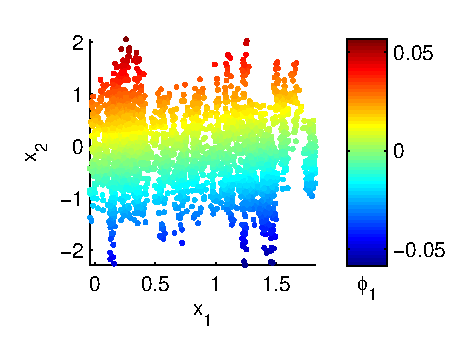
\includegraphics[width=\textwidth]{data_linear_DMAPS}
\caption{}
\label{subfig:NIV_versus_DMAPS1}
\end{subfigure}
\begin{subfigure}{0.45\textwidth}
\centering
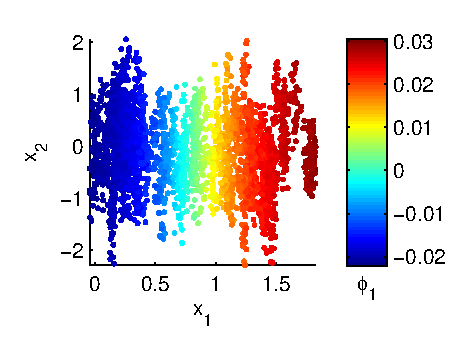
\includegraphics[width=\textwidth]{data_linear_NIV}
\caption{}
\label{subfig:NIV_versus_DMAPS2}
\end{subfigure}
%
\caption[Comparison of using the Euclidean distance and the Mahalanobis distance in analysis of multiscale data]{Comparison of using the Euclidean distance and the Mahalanobis distance in multiscale data mining. (\subref*{subfig:NIV_versus_DMAPS1}) The data from \fig~\ref{fig:initial_data}, colored by the first diffusion map coordinate when using the Euclidean distance in the kernel in \eqref{eq:W}. Note that we do {\em not} recover the slow variable. (\subref*{subfig:NIV_versus_DMAPS2}) The data from \fig~\ref{fig:initial_data}, colored by the first diffusion map coordinate when using the Mahalanobis distance in the kernel in \eqref{eq:W}. The good correspondence between this coordinate and the slow variable is visually obvious.}
\label{fig:NIV_versus_DMAPS}
\end{figure}

\subsubsection{Errors in covariance estimation}

For the example in \eqref{eq:linear_transform}, the analytical covariance is
 \begin{equation} \label{eq:cov_linear_example}
\mathbf{C}(\mathbf{x}(t)) =
\begin{bmatrix}
1 & 0 \\
0 & \frac{1}{\epsilon}
\end{bmatrix}.
\end{equation}
%
From \eqref{eq:cov_error}, we find
%
\begin{equation}
\mathbf{E}_C(\mathbf{x}(t), \delta t) =
\begin{bmatrix}
0 & 0 \\
0 & -\frac{\delta t}{\epsilon^2}
\end{bmatrix}
+ \mathcal{O} (\delta t^{3/2}) .
\end{equation}
%
Therefore, $\| \mathbf{C} \| = \mathcal{O} \left( \frac{1}{\epsilon} \right)$ and $\|\mathbf{E}_C \| = \mathcal{O}\left(\frac{\delta t}{\epsilon^2} \right)$ (provided $\frac{1}{\epsilon^2} \gg \sqrt{\delta t}$; this will be discussed further in \sec~\ref{subsec:fastvar}).
%
These terms are shown in \fig~\ref{fig:cov_error}\subref*{subfig:cov_error1} as a function of $\delta t$.
%
We want to choose $\delta t$ in a regime where $\| \mathbf{E}_C \| \ll \| \mathbf{C} \|$ (the yellow shaded region in \fig~\ref{fig:cov_error} indicates where $\| \mathbf{E}_C \| < \| \mathbf{C} \|$), so that the errors in the estimated covariance are small with respect to the covariance.

When we do not analytically know the functions $\measfn$ or $\mathbf{g}$, we can find such a regime empirically by
estimating the covariance for several values of $\delta t$.
%
This provides an estimate of $\hat{\mathbf{C}} = \mathbf{C} + \mathbf{E}_C$ as a function of $\delta t$.
%
From \fig~\ref{fig:cov_error}\subref*{subfig:cov_error1}, we expect a ``knee" in the plot of $\| \hat{\mathbf{C}} \|$ versus $\delta t$ when $\| \mathbf{E}_C \|$ becomes larger than $\| \mathbf{C}\|$.
%
\fig~\ref{fig:cov_error}\subref*{subfig:cov_error2} shows the empirical $\| \hat{\mathbf{C}} \|$ as a function of $\delta t$ for the data in \fig~\ref{fig:initial_data}, and the knee in this curve is consistent with the intersection in \fig~\ref{fig:cov_error}\subref*{subfig:cov_error1}.

\begin{figure}[t]
\centering
\begin{subfigure}{0.4\textwidth}
\centering
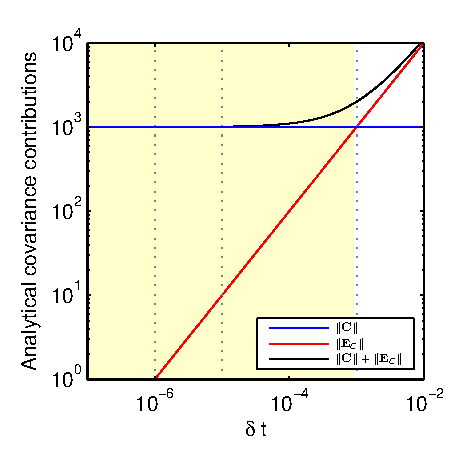
\includegraphics[height=2in]{C_dt_analytical_linear}
\caption{}
\label{subfig:cov_error1}
\end{subfigure}
%
\begin{subfigure}{0.4\textwidth}
\centering
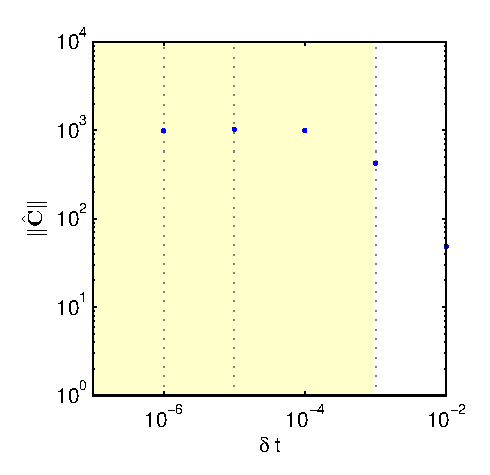
\includegraphics[height=2in]{C_dt_linear}
\caption{}
\label{subfig:cov_error2}
\end{subfigure}
%
\caption[Errors in covariance estimation for linear multiscale example]{Errors in covariance estimation for linear example. (\subref*{subfig:cov_error1}
) The analytical contributions to the covariance for the example in \sec~\ref{subsec:linear_example} as a function of $\delta t$. (\subref*{subfig:cov_error2}) The average estimated covariance $\| \hat{ \mathbf{C}} \|$ as a function of $\delta t$. The average is computed over $10$ data points and using $50$ sample points to estimate each covariance. The shaded yellow region indicates the range of $\delta t$ over which the errors in the estimated covariance are less than the norm of the covariance. }
\label{fig:cov_error}
\end{figure}

\subsubsection{Recovery of the fast variable} \label{subsec:fastvar}

Note that, for the example in \eqref{eq:linear_transform}, $\mathbf{E}_C$ is a constant diagonal matrix.
%
Therefore, taking $\delta t$ too large will not lead to nonlinear effects or mixing of the fast and slow variables.
%
Rather, changing $\delta t$ will only affect the perceived ratio of the fast and slow timescales.

To see this behavior in our diffusion maps results, we must first discuss the interpretation of the diffusion maps eigenspectrum.
%
The diffusion maps eigenvectors provide embedding coordinates for the data, and the corresponding eigenvalues provide a measure of the importance of each coordinate.
%
However, some eigenvectors can be harmonics of previous eigenvectors; for example, for a data set parameterized by a variable $x$, both $\cos x$ and $\cos 2x$ will appear as diffusion maps eigenvectors (see \cite{ferguson2010systematic} for a more detailed discussion).
%
These harmonics do not capture any new direction within the data set, but do appear as additional eigenvector/eigenvalue pairs.
%
Therefore, for the two-dimensional data considered here, the fast variable will not necessarily appear as the second (non-trivial) eigenvector.
%
As the time scale separation increases, the relative importance of the slow and fast directions will also increase.
%
This implies that the eigenvalue corresponding to the eigenvector which parameterizes the fast direction will decrease, and the number of harmonics of the slow mode which appear before the fast mode will increase.

\fig~\ref{fig:recover_fast} shows results for three different values of $\delta t$ (the corresponding values are indicated by the dashed lines in \fig~\ref{fig:cov_error}).
%
When the time scale of the simulation burst used to estimate the local covariance (indicated by the red clouds in the top row of figures), is sufficiently shorter than that of the equilibration time of the fast variable, the estimated local covariance is accurate and the fast variable is collapsed significantly relative to the slow variable.
%
This means that the fast variable is recovered {\em very} far down in the diffusion maps eigenvectors.
%
The left two columns of \fig~\ref{fig:recover_fast} show that, for this example, when the simulation burst is shorter than the equilibration time, the fast variable is recovered as $\phi_{10}$.
%
However, if the time scale of the burst is {\em longer} than the saturation time of the fast variable, the estimated covariance changes: the variance in the slow direction continues to grow, while the variance in the fast direction is fixed.
%
This means that the apparent time scale separation is smaller, the collapse of the fast variable is less pronounced relative to the slow variable, and the fast variable is recovered in an earlier eigenvector (in our ordering of the spectrum).
%
The right column of \fig~\ref{fig:recover_fast} shows that, when the burst is now longer than the equilibration time, the fast variable appears earlier in the eigenvalue spectrum and is recovered as $\phi_6$.

\begin{figure}[!t]
\centering
\def \figwidth {0.28\textwidth}
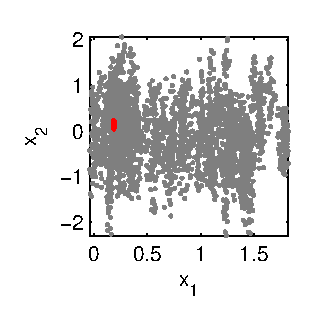
\includegraphics[width=\figwidth]{data_linear_burst1}
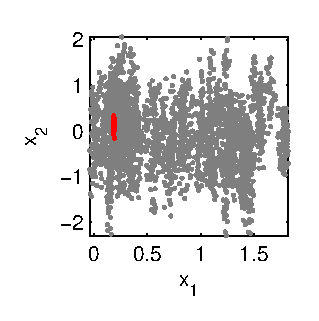
\includegraphics[width=\figwidth]{data_linear_burst2}
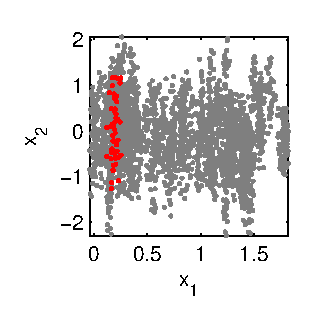
\includegraphics[width=\figwidth]{data_linear_burst3}

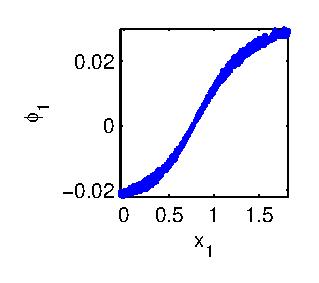
\includegraphics[width=\figwidth]{data_linear_slow1}
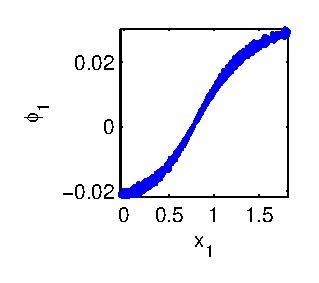
\includegraphics[width=\figwidth]{data_linear_slow2}
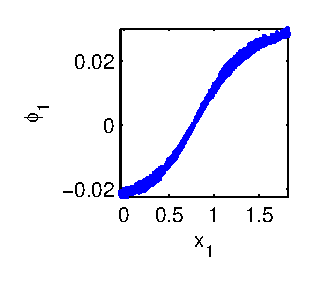
\includegraphics[width=\figwidth]{data_linear_slow3}

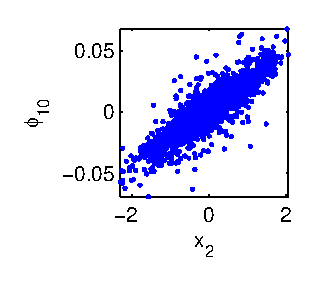
\includegraphics[width=\figwidth]{data_linear_fast1}
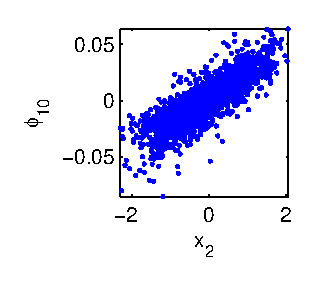
\includegraphics[width=\figwidth]{data_linear_fast2}
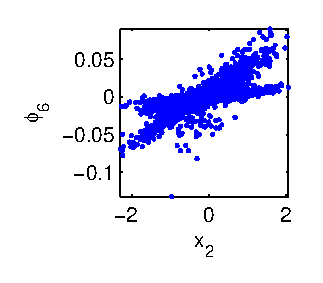
\includegraphics[width=\figwidth]{data_linear_fast3}

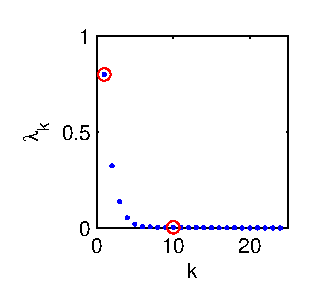
\includegraphics[width=\figwidth]{data_linear_evals1}
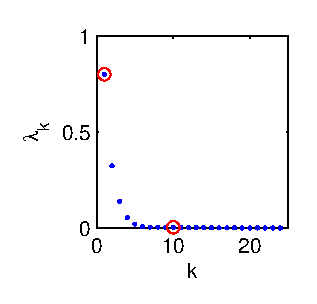
\includegraphics[width=\figwidth]{data_linear_evals2}
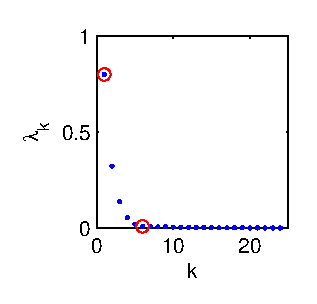
\includegraphics[width=\figwidth]{data_linear_evals3}

\caption[Relationship between changing $\delta t$ and recovery of the variables in analysis of multiscale data]{Relationship between changing $\delta t$ and recovery of the variables. From left to right, the columns correspond to $\delta t = 10^{-6}, 10^{-5}, 10^{-3}$.  (Row~1) Data (gray) and representative burst (red) used to estimate the local covariance. (Row~2) Correlation between first diffusion maps coordinate and the slow variable $x_1$. (Row~3) Correlation between the relevant diffusion maps coordinate and the fast variable $x_2$. Note that for $\delta t = 10^{-6}$ and $\delta t = 10^{-5}$, $x_2$ is correlated with $\phi_{10}$. When $\delta t = 10^{-3}$, $x_2$ is correlated with $\phi_6$. (Row 4) Diffusion maps eigenvalue spectra. The eigenvalues corresponding to the coordinates for the slow and fast modes are indicated by red circles. Note that when $\delta t$ is too large, the apparent time scale separation decreases and the coordinate corresponding to the fast variable appears earlier in the spectrum. }
\label{fig:recover_fast}
\end{figure}

\subsection{Nonlinear observation function} \label{subsec:nonlinear_example}

In the second example, our data will be warped into ``half-moon" shapes via the function
\begin{equation} \label{eq:nonlinear_function}
\begin{aligned}
\begin{bmatrix}
y_1(t) \\ y_2(t)
\end{bmatrix} &=&
\measfn(\mathbf{x}(t)) &=&
\begin{bmatrix}
x_1(t) + x_2^2(t) \\
x_2(t)
\end{bmatrix}\\
\mathbf{g}(\data(t)) &=& \measfn^{-1} (\data(t)) &=& \begin{bmatrix} y_1(t) - y_2^2(t) \\ y_2(t) \end{bmatrix} .
\end{aligned}
\end{equation}
%
\fig~\ref{fig:initial_data_nonlinear} shows the data from \fig~\ref{fig:initial_data} transformed by the function $\measfn$ in \eqref{eq:nonlinear_function} and colored by time.
%
It is important to note that this is a difficult class of problem in practice, as none of the observed
variables are purely fast or slow, and the observed system appears, at first inspection, to possess no separation
of time scales.
%
For this example, the analytical covariance and inverse covariance are
\begin{equation}
\begin{aligned}
\mathbf{C}(\mathbf{x}(t)) =&
\frac{1}{\epsilon}
 \begin{bmatrix}
\epsilon + 4x_2^2(t) & 2x_2(t) \\
2x_2(t) & 1
\end{bmatrix}\\
\mathbf{C}^{\dagger}(\mathbf{x}(t)) =&
\begin{bmatrix}
1 & -2 x_2(t) \\
-2 x_2(t) & \epsilon+ 4 x_2^2(t)
\end{bmatrix} .
\end{aligned}
\end{equation}

The fast and slow variables are now coupled through the function $\measfn$, and the Euclidean distance is not informative about the fast {\em or} the slow variables.
%
We need to use the Mahalanobis distance to obtain a parametrization that is consistent with the underlying fast-slow dynamics.

\begin{figure}[t]
\centering
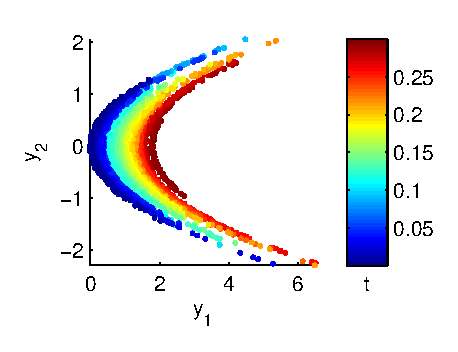
\includegraphics[width=0.5\textwidth]{data_init_nonlinear}
%
\caption[Nonlinear multiscale data]{The data from \fig~\ref{fig:initial_data}, transformed by $\measfn$ in \eqref{eq:nonlinear_function}}
\label{fig:initial_data_nonlinear}
\end{figure}

\subsubsection{Errors in Mahalanobis distance}

We can bound the Mahalanobis distance by the eigenvalues of $\mathbf{C}^{\dagger}$,
\begin{equation}
\lambda_{C^{\dagger},1} \| \data(t_2) - \data(t_1) \|_2^2
\le
\| \data(t_2) - \data(t_1) \|^2_M
\le
\lambda_{C^{\dagger},2} \| \data(t_2) - \data(t_1) \|_2^2
\end{equation}
where $\lambda_{C^{\dagger},1} \le \lambda_{C^{\dagger},2}$ are the two eigenvalues of $\mathbf{C}^{\dagger}$.
%
Therefore, for the example in \eqref{eq:nonlinear_function}, we have
\begin{equation}
E_M(\data(t_1), \data(t_2)) = - (y_2(t_2) - y_2(t_1))^4.
\end{equation}

\fig~\ref{fig:cov_error_nonlinear}\subref*{subfig:dist_error_nonlinear1} shows $\| \data(t_2) - \data(t_1) \|^2_M$ and $| E_M |$ as a function of $\| \data(t_2) - \data(t_1) \|_2$.
%
The Mahalanobis distance is an accurate approximation to the true intrinsic distance $\| \mathbf{z}(t_2) - \mathbf{z}(t_1) \|_2$ when $|E_M| \ll \| \data(t_2) - \data(t_1) \|^2_M$ (the shaded yellow region in the plot indicates where $|E_M| < \| \data(t_2) - \data(t_1) \|^2_M$).
%
We want to choose $\sigma_{kernel}^2$ in a regime where $|E_M(\data(t_1), \data(t_2))| \ll \| \data(t_2) - \data(t_1) \|^2_M$, so that the distances we utilize in the diffusion maps calculation are accurate.
%
We can find such a regime empirically by plotting $\| \data(t_2) - \data(t_1) \|^2_M$ as a function of $\| \data(t_2) - \data(t_1) \|_2$, and assessing when the relationship deviates from quadratic.
%
This is shown in \fig~\ref{fig:cov_error_nonlinear}\subref*{subfig:dist_error_nonlinear2}, and the deviation from quadratic behavior is consistent with the intersection of the analytical expressions plotted in \fig~\ref{fig:cov_error_nonlinear}\subref*{subfig:dist_error_nonlinear1}.

\fig~\ref{fig:colored_data_nonlinear_cases} shows the data from \fig~\ref{fig:initial_data_nonlinear}, colored by $\phi_1$ for two different values of $\dmeps$.
%
The corresponding values of $\dmeps^2$ are indicated by the dashed lines.
%
When $\dmeps^2$ corresponds to a region where $ |E_M | \ll \|\data(t_2) - \data(t_1) \|_M^2$, $\phi_1$ is well correlated with the slow variable.
%
However, when $\dmeps^2$ corresponds to a region where $|E_M | \gg \|\data(t_2) - \data(t_1) \|_M^2$, the slow variable is no longer recovered.

\begin{figure}[t]
\centering
\begin{subfigure}{0.4\textwidth}
\centering
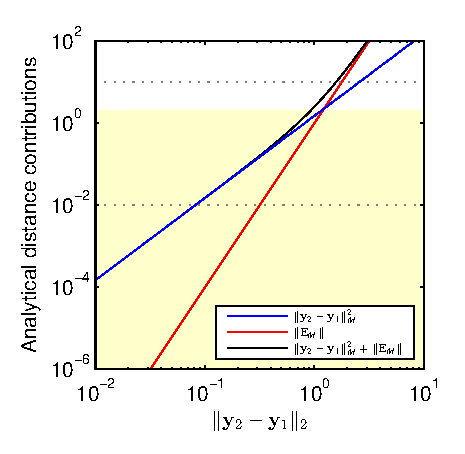
\includegraphics[height=2in]{dist_dy_analytical_nonlinear}
\caption{}
\label{subfig:dist_error_nonlinear1}
\end{subfigure}
%
\begin{subfigure}{0.4\textwidth}
\centering
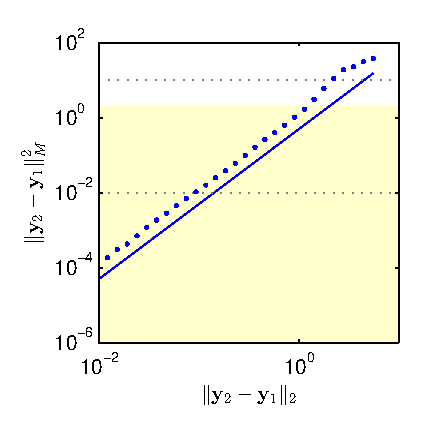
\includegraphics[height=2in]{dist_dy_nonlinear}
\caption{}
\label{subfig:dist_error_nonlinear2}
\end{subfigure}

\begin{subfigure}{0.4\textwidth}
\centering
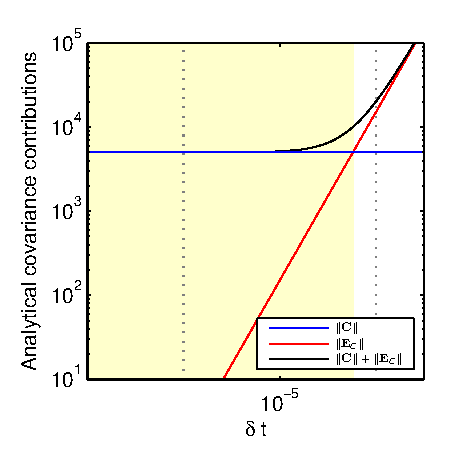
\includegraphics[height=2in]{C_dt_analytical_nonlinear}
\caption{}
\label{subfig:cov_error_nonlinear1}
\end{subfigure}
%
\begin{subfigure}{0.4\textwidth}
\centering
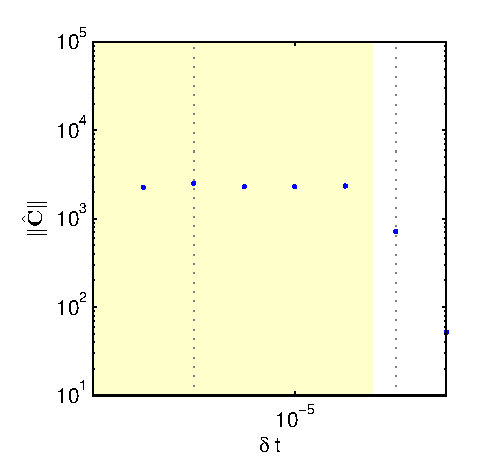
\includegraphics[height=2in]{C_dt_nonlinear}
\caption{}
\label{subfig:cov_error_nonlinear2}
\end{subfigure}
%
\caption[Errors in the Mahalanobis distance and the covariance estimation for nonlinear multi scale data]{Errors in the Mahalanobis distance and the covariance estimation for the nonlinear example in \eqref{eq:nonlinear_function}. (\subref*{subfig:dist_error_nonlinear1}) The analytical expressions for the contributions to the distance approximation as a function of $\| \data_2 - \data_1\|_2$. (\subref*{subfig:dist_error_nonlinear2}) The average estimated Mahalanobis distance $\| \data_2 - \data_1\|^2_M$ as a function of the distance $\| \data_2 - \data_1\|_2$. The line $\| \data_2 - \data_1\|^2_M = \| \data_2 - \data_1\|_2$ is shown for reference. The yellow region indicates the range in which $\sigma_{kernel}$ should be chosen. (\subref*{subfig:cov_error_nonlinear2}) The analytical expressions for the contributions to the covariance as a function of $\delta t$. (\subref*{subfig:cov_error_nonlinear2}) The average estimated covariance $\| \hat{\mathbf{C}} \|$ as a function of $\delta t$. The yellow region indicates the range of $\delta t$ over which the errors in the estimated covariance are small relative to the norm of the covariance. }
\label{fig:cov_error_nonlinear}
\end{figure}

\subsubsection{Errors in covariance estimation}

From \eqref{eq:cov_error}, we find that, for the example in \eqref{eq:nonlinear_function},
%
\begin{equation}
\begin{aligned}
E_{C,11} (\mathbf{x}(t), \delta t)
=&
\frac{2 \delta t}{\epsilon^2}
- \frac{8 x_2(t)}{\epsilon^2 \delta t} \mathbb{E} \left[ \int_t^{t+\delta t} \left( \int_{s_2}^{t+\delta t} 2 x_2(s_1) ds_1
+  \int_t^{s_2} x_2(s_1) ds_1 \right) ds_2\right]  \\ &+ \mathcal{O} (\delta t^{3/2}) \\
%%
E_{C, 12} (\mathbf{x}(t), \delta t)
= &
E_{C, 21} (\mathbf{x}(t), \delta t)\\
=&
- \frac{x_2(t) \delta t}{\epsilon^2}
- \frac{2}{\epsilon^2 \delta t} \mathbb{E} \left[ \int_t^{t+\delta t} \left( \int_{s_2}^{t + \delta t} 2 x_2(s_1) ds_1 + \int_t^{s_2} x_2(s_1) ds_1 \right) ds_2 \right] \\ &+ \mathcal{O} (\delta t^{3/2})\\
%%
E_{C, 22} (\mathbf{x}(t), \delta t)
=&
-\frac{\delta t}{\epsilon^2} + \mathcal{O} (\delta t^{3/2})
\end{aligned}
\end{equation}
%
The error in the covariance is $\mathcal{O} \left( \frac{\delta t}{\epsilon^2} \right)$.
%
As expected, the error grows with increasing $\delta t$.
%
We can also see the explicit dependence of the covariance error on the time scale separation $\epsilon$; larger time scale separation results in a larger covariance error, as a more refined simulation burst is required to estimate the covariance of the fast directions.
%
$\|\mathbf{C} \|$ and $\| \mathbf{E}_C\|  $ are plotted as a function of $\delta t$ in \fig~\ref{fig:cov_error_nonlinear}\subref*{subfig:cov_error_nonlinear1}; the shaded yellow portion denotes the region where $\| \mathbf{E}_C \| < \| \mathbf{C} \|$.
%
As in the previous example, we can empirically find where $\| \mathbf{E}_C \| \ll \| \mathbf{C} \|$  by plotting $\| \hat{\mathbf{C}} \|$ as a function of $\delta t $ and looking for a knee in the plot.
%
These results are shown in \fig~\ref{fig:cov_error_nonlinear}\subref*{subfig:cov_error_nonlinear2}.

\fig~\ref{fig:colored_data_nonlinear_cases} shows the data from \fig~\ref{fig:initial_data_nonlinear}, colored by $\phi_1$ for two different values of $\delta t$.
%
The corresponding values of $\delta t$ are indicated by the dashed lines in \fig~\ref{fig:cov_error_nonlinear}\subref*{subfig:cov_error_nonlinear1},\subref*{subfig:cov_error_nonlinear2}.
%
When $\delta t$ corresponds to a region where $\|\mathbf{E}_C \| \ll \| \mathbf{C} \|$, the slow variable is recovered by the first diffusion maps coordinate.
%
However, when $\delta t$ corresponds to a region where $\|\mathbf{E}_C \| \gg \| \mathbf{C} \|$, the slow variable is no longer recovered.


\def \figheight {1.5in}

\begin{figure}[t]

\begin{subfigure}{\textwidth}
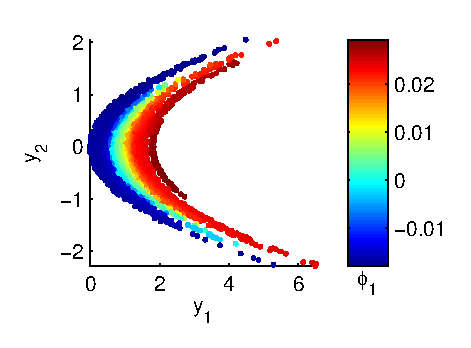
\includegraphics[height=\figheight]{data_nonlinear_NIV_dt1_kernel1}
\hfill
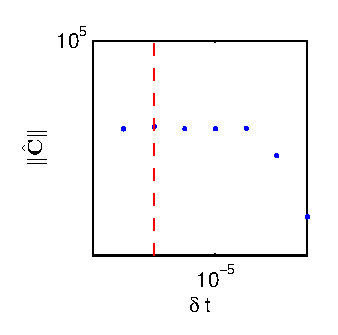
\includegraphics[height=\figheight]{C_dt_nonlinear_dt1_kernel1}
\hfill
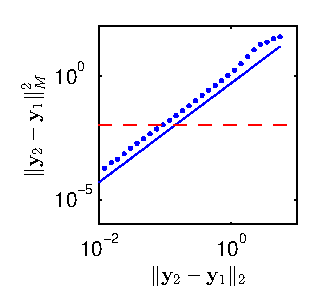
\includegraphics[height=\figheight]{dist_dy_nonlinear_dt1_kernel1}
\end{subfigure}

\begin{subfigure}{\textwidth}
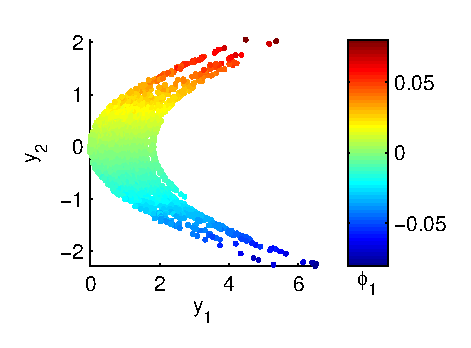
\includegraphics[height=\figheight]{data_nonlinear_NIV_dt1_kernel2}
\hfill
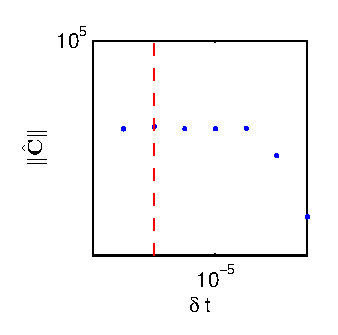
\includegraphics[height=\figheight]{C_dt_nonlinear_dt1_kernel2}
\hfill
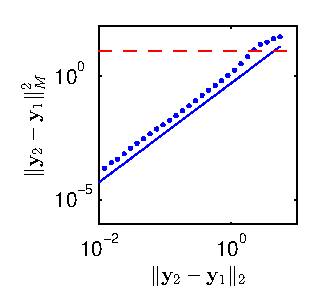
\includegraphics[height=\figheight]{dist_dy_nonlinear_dt1_kernel2}
\end{subfigure}

\begin{subfigure}{\textwidth}
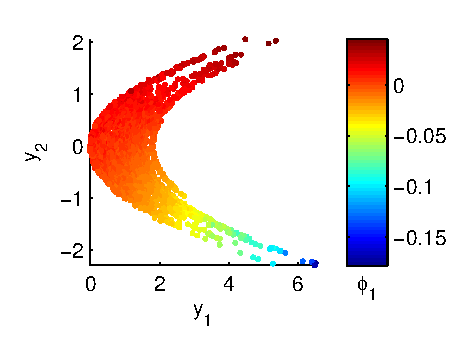
\includegraphics[height=\figheight]{data_nonlinear_NIV_dt2_kernel1}
\hfill
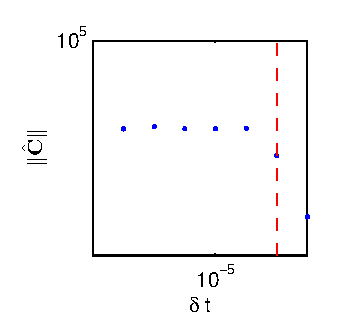
\includegraphics[height=\figheight]{C_dt_nonlinear_dt2_kernel1}
\hfill
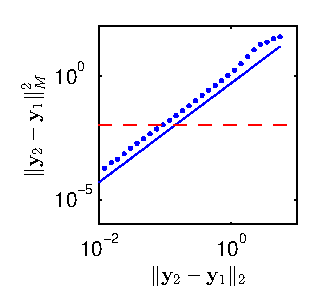
\includegraphics[height=\figheight]{dist_dy_nonlinear_dt2_kernel1}
\end{subfigure}

\caption[Analysis of nonlinear multiscale data for different parameter settings]{Data from \fig~\ref{fig:initial_data_nonlinear}, colored by the first diffusion maps variable $\phi_1$ using the Mahalanobis distance for three different parameter settings. The relevant values of $\delta t$ and $\sigma_{kernel}$ are indicated by the red dashed lines on the corresponding plots.  (Row~1) $\delta t = 10^{-7}$ and $\sigma_{kernel}^2 = 10^{-2}$. Note that the parametrization is one-to-one with the slow variable.  (Row~2) $\delta t = 10^{-7}$ and $\sigma_{kernel}^2 = 10^{1}$. We do not recover the slow variable because $\sigma_{kernel}$ is too large. (Row~3)  $\delta t = 10^{-3}$ and $\sigma_{kernel}^2 = 10^{-2}$. We do not recover the slow variable because $\delta t$ is too large.  }
\label{fig:colored_data_nonlinear_cases}
\end{figure}


\section{Discussion}

We have presented a methodology to compute a parametrization of a data set which respects the slow variables in the underlying dynamical system.
%
The approach utilizes diffusion maps, a kernel-based manifold learning technique, with the Mahalanobis distance as the metric.
%
We showed that the Mahalanobis distance collapses the fast directions within a data set, allowing for successful recovery of the slow variables.
%
Furthermore, we showed how to estimate the covariances (required for the Mahalanobis distance) directly from data.
%
A key point in our approach is that the embedding coordinates we compute are not only insensitive to the fast variables, but are also invariant to nonlinear observation functions.
%
Therefore, the approach can be used for data fusion: data collected from the same system via different measurement functions can be combined and merged into a single coordinate system.

In the examples presented, the initial data came from a single trajectory of a dynamical system, and the local covariance at each point in the trajectory was estimated using brief simulation bursts.
%
However, the initial data need not be collected from a single trajectory, and other sampling schemes could be employed.
%
Brief time series are required to estimate the local covariances, but given a simulator, one could reinitialize brief simulation bursts which are sufficiently short and refined from each sample point.

In our examples, we controlled the time scale of sampling and could therefore set the time scale over which to estimate the covariance and the simulation time step arbitrarily small.
%
However, in some settings, such as previously collected historical data, it is not uncommon to have a fixed sampling rate and be unable to reinitialize simulations.
%
In such cases, it is possible that we cannot find an appropriate kernel scale given the fixed $\delta t$ such that we can accurately recover the slow variables.
%
For these cases, the data cannot be processed as given,
and it is necessary to construct intermediate observers,
such as histograms, Fourier coefficients, or scattering transform coefficients \cite{mallat2012group, talmon2014intrinsic, talmon2014manifold}.
%
Such intermediates are more complex statistical functions than simple averages and can capture additional structure within the data.
%
They also reduce the effects of noise and permit a larger time step.
%
However, constructing such intermediates often requires additional {\em a priori} knowledge about the system dynamics and noise structure.

Clearly, in our analysis, we have ignored the finite sampling effects in our estimation.
%
In reality, both the number of samples used to estimate the covariances, as well as the density of sampled points on the manifold, affect the recovered parametrization and provide additional constraints on $\delta t$ and $\dmeps$.
%
Future work involves extending our analysis to the finite sample case, and providing guidelines for the amount of data required to apply our methodology.

The methods presented here provide a bridge between traditional data mining and multiple time scale dynamical systems.
%
With this interface established, one can now consider using such data-driven methodologies to extract reduced models (either explicitly, or implicitly via an equation-free framework \cite{erban2006gene, kevrekidis2004equation, kevrekidis2003equation,  kevrekidis2009equation}) which also respect the underlying slow dynamics and geometry of the data.
%
Such reduced models hold the promise of accelerated analysis and reduced simulation of dynamical systems whose effective dynamics are obscure upon simple inspection.
%
In the following chapter, we will exploit another feature of the Mahalanobis distance (its invariance to measurement/observation functions) to analyze and merge multiple data sets. 

% !TEX root = ../thesis.tex

\chapter{Merging Data from Different Observations of Dynamical Systems \label{ch:merging}}

\graphicspath{{ch-merging/figures/}}

{\em This work was published in \citep{dsilva2013nonlinear}.}

\section{Introduction}

From the discussions in \chap~\ref{ch:intro}~and~\ref{ch:multiscale}, the benefits from constructing reduced descriptions of data are clear; however, a crucial shortcoming of
 data-driven reduction coordinates is their dependence on the specific data set processed,
and not only on the physical model in question.
%
It is well known that, even in the simple linear case of principal component analysis \cite{jolliffe2005principal},
different data sets on the same low-dimensional hyperplane in the ambient space
will lead to different bases spanning the hyperplane - in effect, to different reduction coordinates $\mathbf{x}$.
%
While this can be easily rectified by an affine transformation
(see, by analogy, the discussion in Lafon {\em et al.}\cite{lafon2006data}),
the problem becomes
exacerbated when the low-dimensional space is curved (a manifold, rather than a hyperplane)
and when different data sets are obtained using different instrumental modalities
(such as when one wants to merge molecular dynamics data with, for example, spectral information).
%

In this work, we propose a new method to embed data in a low-dimensional space.
%
This method is based on a kernel constructed from a Riemannian metric that is specially designed to exploit the noise/diffusion induced variability of the data in local neighborhoods.
%
By solving the appropriate eigenvector problem, local affinities from the kernel are integrated into a global coordinate system for the data.

We will demonstrate this can produce a {\em unique} and {\em consistent} reduction
coordinate set, shared by all measurement ensembles and observation modalities.
%
We will call these coordinates Nonlinear Intrinsic Variables.
%
Embedding data in such a coordinate system allows us to naturally merge different observations of the same system;
more importantly, it enables the construction of an empirical mapping between these different
observation ensembles, allowing us to complete partial measurements in a test data set from a training data set
that consists of {\em different} observations.
%
To construct this empirical mapping and the associated observers,
accurate interpolation tools must be available in the embedding space; to this
end, we will demonstrate the use of a multiscale Laplacian Pyramid approach \cite{rabin2012heterogeneous}.

We will illustrate our methodologies with two distinct examples.
%
The first is a simulation
of two Goldbeter-Koshland modules in an enzyme kinetics model using the Gillespie Stochastic Simulation
Algorithm (SSA) \cite{gillespie1977exact};
in certain parameter regimes, separation of time scales is known
to reduce the ODE model of this kinetic scheme to an effective two-dimensional description \cite{zagaris2012stability}.
%
Although this example is rather simple, it will serve as an introduction to our techniques and highlight the main features of the algorithms.
%
The second example is a molecular dynamics
simulation (in explicit water) of a simple peptide fragment (alanine dipeptide) whose folding
dynamics are known to be described through a small set of physical observables \cite{bolhuis2000reaction}.
%
This example will allow us to compare our approach to more common techniques,
such as diffusion maps \cite{coifman2005geometric} for dimensionality reduction
and nearest neighbor interpolation for observation reconstruction.
%
The remainder of the chapter is structured as follows: in \sec~\ref{sec:NIV} we present the Nonlinear Intrinsic Variable formulation and
the associated inference method.
%
\sec~\ref{sec:LapPyr} contains our discussion of Laplacian Pyramids that
is used for the completion of partial observations.
%
In \sec~\ref{sec:examples}, the results
of the application of the approach to simulation data from our two illustrative examples are presented and discussed.
%
We conclude with a summary and our perspective on open issues in \sec~\ref{sec:conclusions}.

\section{Nonlinear Intrinsic Variables} \label{sec:NIV}

\subsection{Problem formulation}
Let $\data(t)$ be a high-dimensional measured process in $\mathbb{R}^\highdim$ consisting of $\highdim$ observable variables.
%
We impose two critical assumptions. First, the measured process is assumed to be a manifestation in an observable domain of a low-dimensional diffusion process. Thus, it can be expressed by
\begin{equation}
	\data(t) = \measfn(\mathbf{x}(t)),
\end{equation}
where $\measfn:\mathbb{R}^\lowdim \rightarrow \manifold$ is an unknown (possibly nonlinear) function, $\manifold \subset \mathbb{R}^\highdim$ is a $\lowdim$-dimensional manifold,
and $\mathbf{x}(t)$ is a diffusion process that consists of $\lowdim$ underlying variables (with $\lowdim \ll \highdim$).
%
Second, the dynamics of the diffusion process in each of its underlying variables are described by normalized stochastic differential equations as
\begin{equation}
	d x_i(t) = a_i (\mathbf{x}(t)) dt + d W_i(t), \ i=1,\ldots,\lowdim,
	\label{eq:dynamics}
\end{equation}
where $a_i$ are unknown drift functions and $\dot{W}_i(t)$ are independent white noises.
%
The independence is our second critical assumption.

Given a sequence of samples $\data(t), \ t=1,\ldots,T$, we present an empirical method to construct a unique and consistent reduction coordinate set, represented here by $\mathbf{x}(t)$ \cite{singer2008non}.
%
Because the empirical method we will describe is independent of the observation function $\measfn$,
we refer to the coordinates of $\mathbf{x}(t)$ as Nonlinear Intrinsic Variables (NIV).
%
The available samples $\data(t)$ may be the result of different measurement functions $\measfn$ in various observable domains,
or they may be partial measurements consisting of merely a subset of the coordinates of the observable domains.
%
The idea is to empirically construct a NIV coordinate system driven entirely by measurements that is invariant to the observation function $\measfn$
(see Figure \ref{fig:IntrinsicIllustration} for a schematic illustration).
%
We remark that the available data should be ``rich enough'', i.e., consist of a sufficient amount of historical data with adequate variability, in order to obtain the full empirical model;
this is further discussed and demonstrated in the experimental study.

The method consists of the following main principles.
%
(1) The underlying diffusion process implies that a short trajectory of successive samples mainly consists of diffusion noise,
and hence, creates a ``sphere" of samples in the underlying domain $\mathbb{R}^\lowdim$.
%
This sphere is mapped to an ellipse in the observable domain by the measurement function $\measfn$.
%
In this work, the identification of the associated ellipse of samples according to the time trajectory of our data enables us
to estimate the tangent planes of the observable manifolds {\em via the principal components of the covariance matrices of the samples in these ellipses}.
%
(2) The principal directions of the tangent planes are utilized to define a Riemannian metric that is shown to be {\em locally invariant to the measurement function $\measfn$}.
%
(3) The NIV are constructed through the eigenvalue decomposition of a Laplace operator that is built upon a pairwise affinity between the samples, defined using this Riemannian metric.

\begin{figure*}[ht]
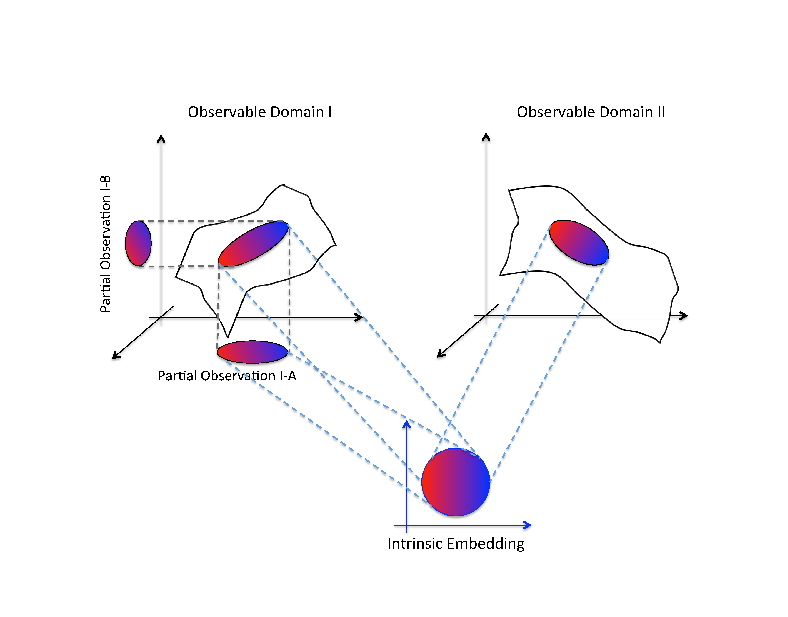
\includegraphics[width=5in]{fig1}
\caption[Illustration of the underlying theory in nonlinear intrinsic variables]{Illustration of the nonlinear embedding that yields an intrinsic representation independent of the measurement function $\measfn$. (Bottom) The underlying variables in which the noises are independent with unit variance. The circle illustrates samples from, say, a short trajectory in time that sample a disc on the manifold. (Top Left) The first set of observed variables. The ellipse illustrates the mapping of the sphere of the underlying samples into the observable domain via the first observation function. In this sketch, we illustrate that the observations might be {\em partial}, i.e., might consist of merely a subset of the observed domain variables. (Top Right) Second set of observable variables. The ellipse illustrates the mapping of the sphere of the underlying samples into this (different) observable domain via a second observation function.
\label{fig:IntrinsicIllustration}}
\end{figure*}

\subsection{Diffusion maps and the Mahalanobis distance}
\label{subsec:mahalanobis}

We use the Mahalanobis distance in \eqref{eq:mahalanobis1}, with the covariance estimation in \eqref{eq:cov1}, to compare pairs of data points.
%
%Let $\mathbf{C}(t)$ be the covariance matrix associated with the measured sample $\mathbf{Y}(t)$. In practice, the covariance matrix can be estimated from a short trajectory of samples in time around the sample $\mathbf{Y}(t)$ by
%\begin{equation}
%	\widehat{\mathbf{C}}(t) = \sum \limits _{\tau = t-L}^{t+L} (\mathbf{Y}(\tau) - \widehat{\boldsymbol{\mu}}(t))(\mathbf{Y}(\tau) - \widehat{\boldsymbol{\mu}}(t))^T,
%	\label{eq:cov}
%\end{equation}
%where $\widehat{\boldsymbol{\mu}}(t)$ is the empirical mean of the short trajectory of samples.
%%
%We define a Riemannian metric between a pair of samples using the associated covariance matrices as
%\begin{equation}
%	d^2(\mathbf{Y}(t), \mathbf{Y}(\tau)) = 2 (\mathbf{Y}(t) - \mathbf{Y}(\tau))^T(\widehat{\mathbf{C}}(t) + \widehat{\mathbf{C}}(\tau))^{\dagger}(\mathbf{Y}(t) - \mathbf{Y}(\tau));
%	\label{eq:mahalanobis}
%\end{equation}
%this is the Mahalanobis distance (and $^{\dagger}$ denotes a pseudoinverse, as discussed below).
%%
%As previously described, the covariance matrices convey the local variability of the measurements and are utilized to explore and learn the tangent planes of the observable manifold.
%%
%This information is then utilized in \eqref{eq:mahalanobis} to compare a pair of points according to the directions of their respective tangent planes.
%
The Mahalanobis distance is invariant under affine transformations.
%
Thus, by assuming that the observation function $\measfn$ is bi-Lipschitz and smooth, and by using local linearization of the function, i.e., $\data(t) = \mathbf{J}(t) \mathbf{x}(t) + \boldsymbol{\epsilon}(t)$ where $\mathbf{J}(t)$ is the Jacobian of $\measfn(\mathbf{x}(t))$ and $\boldsymbol{\epsilon}(t)$ is the residual consisting of higher-order terms, it was shown by Singer and Coifman \cite{singer2008non} that $\mathbf{C}(t) = \mathbf{J}(t)\mathbf{J}^T(t)$ and that the Mahalanobis distance approximates the Euclidean distance between the corresponding samples of the underlying process to second order, i.e.,
\begin{equation}
	\| \mathbf{x}(t) - \mathbf{x}(\tau) \|^2_M = \| \data(t) - \data(\tau)\|^2_2 + \mathcal{O}(\| \data(t) - \data(\tau)\|_2^4).
\end{equation}
%
This result implies that the Mahalanobis distance is invariant to the measurement function $\measfn$, and hence,
it yields the same distances between samples obtained under different observation functions or even partial observations.
%
We would like to note that, in general, $\measfn$ being bi-Lipschitz implies that $\measfn$ is invertible (on the $\lowdim$-dimensional
manifold $\manifold$).
%
However, in practice, determining whether $\measfn$ contains sufficient information and is ``rich enough'' to completely determine the underlying process is a non-trivial task.
%
In this work, we exploit the fact that $\mathbf{C}(t) = \mathbf{J}(t)\mathbf{J}^T(t)$, which implies that $\mathbf{C}(t)$ is an $\highdim \times \highdim$ positive semidefinite matrix of rank $\lowdim$, to empirically infer the dimension $\lowdim$.
%
According to the spectrum of the local covariance matrices and their corresponding spectral gaps, we approximate the rank of the matrices.
%
Consistent rank estimates among these local covariance matrices are taken to imply that the measurements are ``rich enough", and hence, may be good indicators for the dimension $\lowdim$.
%
Since the dimension $\lowdim$ of the underlying process is typically considerably smaller than the dimension of the measured process $\highdim$,
the covariance matrix is singular and non-invertible;
%
thus, we use the pseudo-inverse in \eqref{eq:mahalanobis1}.

%\subsection{Laplace Operator}

The Mahalanobis distance described in \sec~\ref{sec:mahalanobis} enables us to compare observations in terms of the intrinsic variables of the associated underlying diffusion process.
%
We then use diffusion maps, with the Mahalanobis distance in the kernel matrix in \eqref{eq:W} and $\dmeps$ as the median of the pairwise distances, to obtain a parameterization our data with respect to the intrinsic variables $\mathbf{x}$.
%
%In this section, we show how to recover the underlying process itself from the pairwise Euclidean distances through the eigenvectors of a Laplace operator.
%
%Let $\mathbf{W}$ be a pairwise affinity matrix (kernel) based on a Gaussian, whose $(t,\tau)$-th element is given by
%\begin{equation}
%	W_{t,\tau} = \exp \left\{ - \frac{ d^2(\mathbf{Y}(t), \mathbf{Y}(\tau) )} {\varepsilon}\right\},
%	\label{eq:kernel}
%\end{equation}
%where $\varepsilon$ is the kernel scale, which can be set according to Hein and Audibert \cite{hein2005intrinsic} and Coifman {\em et al.} \cite{coifman2008graph}.
%%
%Based on the kernel, we form a weighted graph, where the measurements $\mathbf{Y}(t)$ are the graph nodes and the weight of the edge connecting node $\mathbf{Y}(t)$ to node $\mathbf{Y}(\tau)$ is $W_{t,\tau}$.
%%
%In particular, a Gaussian kernel exhibits a notion of locality by defining a neighborhood around each measurement $\mathbf{Y}(t)$ of radius $\varepsilon$,
%i.e., measurements $\mathbf{Y}(\tau)$ such that $d^2(\mathbf{Y}(t), \mathbf{Y}(\tau) ) > \varepsilon$ are weakly connected to $\mathbf{Y}(t)$.
%%
%In practice, we set $\varepsilon$ to be the median of the pairwise distances.
%%
%According to the graph interpretation, this implies a well-connected graph because each measurement is effectively connected to half of the other measurements \cite{rohrdanz2011determination}.
%
%Let $\mathbf{D}$ be a diagonal matrix whose elements are the row sums of $\mathbf{W}$, and let
%\begin{equation}\label{eq:kernel}
%\mathbf{W}^{\mathrm{norm}} = \mathbf{D}^{-1/2}\mathbf{W}\mathbf{D}^{-1/2}
%\end{equation}
%be a normalized kernel that shares its eigenvectors with the normalized graph-Laplacian $\mathbf{I}-\mathbf{W}^{\mathrm{norm}} \:$ \cite{chung1997spectral}.
%%
%The diagonal entries of $D$ serve as estimates for the density of data around each point.
%%
%The eigenvectors of $\mathbf{W}^{\mathrm{norm}}$, denoted $\psi_j$, reveal the underlying structure of the data \cite{coifman2005geometric}.
%%
%Specifically, the $i$-th coordinate of the $j$-th eigenvector can be associated with an intrinsic coordinate $j$ of the sample $\mathbf{x}(i)$ of the underlying process.
%%
%The eigenvectors are ordered such that $|\lambda_1| \ge |\lambda_2| \ge \dots \ge |\lambda_n|$, where $\lambda_j$ is the eigenvalue associated with eigenvector $\psi_j$.
%%
%Because $\mathbf{W}^{\mathrm{norm}} \sim \mathbf{D}^{-1}\mathbf{W} $, and $\mathbf{D}^{-1}\mathbf{W}$ is row-stochastic,
%$\lambda_1 = 1$ and $\psi_1$ is the diagonal of $\mathbf{D}^{1/2}$.
%%
%The next few eigenvectors can be argued to describe the geometry of the underlying manifold \cite{coifman2005geometric}.
%%
%However, some eigenvectors can be higher harmonics of the same principal direction along the data manifold.
%This is analogous to how the eigenfunctions $\cos x$ and $\cos 2x$ of the usual Laplacian in one spatial dimension
%and with no flux boundary conditions are one-to-one with the values of $x$ for $0 \le x \le 1$;
%one must check for correlations between the eigenvectors before selecting those that describe the underlying manifold geometry.
%%
%The above steps to construct the nonlinear intrinsic variables are summarized in Algorithm \ref{algo}.
%
%Ignoring the higher harmonics, each retained eigenvector then describes an intrinsic variable for the data set of interest.
%%
%%Because eigenvectors can be determined up to a scaling factor,
%We must normalize the eigenvectors from different data sets so that the resulting embeddings are consistent.
%%
%We first scale the eigenvectors so that $\|\psi_i\| = T$, where $T$ is the number of data points,
%to make the embedding coordinates invariant to the size of the data set.
%%twice as many samples as another data set, but with the same underlying geometry, should have twice the norm.
%%
%Still, the computed embedding eigenvectors, even for two identical data sets, may differ by a sign.
%%
%Reconciling the signs for the embeddings of different data sets can be rationally done in several ways and is somewhat problem-specific.
%%
%For example, if the mean of the embedding is sufficiently far from 0, we can require $\langle \psi_i \rangle > 0$;
%alternatively, if there is a common region sampled by both data sets, the sign of each eigenvector can be chosen to optimize the consistency of the embeddings of the common region data.
%%
%We will return to the issue of embedding consistency for different data sets in our concluding discussion; for the moment,
%we will assume that our different sets sample the same region of data space in a representative enough way such that the
%correspondence between the sequences of retained eigenvectors for different embeddings is obvious.
%
%\begin{table}[th!]
%\caption{Nonlinear Intrinsic Variables Construction}
%\begin{enumerate}
%
%\item
%Obtain a sequence of high-dimensional observation samples $\mathbf{Y}(t)$.
%
%\item
%Compute the empirical covariance matrix $\widehat{\mathbf{C}}(t)$ of each sample $\mathbf{Y}(t)$ {\em in a short window in time} according to \eqref{eq:cov}.
%
%\item
%Using the samples and their associated covariance matrices, compute the Mahalanobis distance between the observations \eqref{eq:mahalanobis} .
%
%\item
%Build the pairwise affinity matrix $\mathbf{W}$ and the corresponding normalized kernel $\mathbf{W}^{\mathrm{norm}}$ (\ref{eq:kernel}).
%
%\item
%Apply eigenvalue decomposition to the normalized kernel and view the values of its principal eigenvectors (modulo the possibility of
% ``higher harmonics", see text) as the Nonlinear Intrinsic Variables (NIV) of the given observations.
%
%\end{enumerate}
%\hrule
%\label{algo}
%\end{table}
%
%\subsection{Limiting Diffusion Operator} \label{sec:diff_limit}
%
%Assume that the dynamics of the underlying variables in \eqref{eq:dynamics} can be rewritten as
%\begin{equation} \label{eq:Langevin}
%	d\mathbf{x}(t) = - \nabla U(\mathbf{x}(t)) dt + d \mathbf{w}(t),
%\end{equation}
%where the drift term is expressed as a gradient of a potential $U$ and $\dot{\mathbf{w}}(t) \in \mathbb{R}^d$ is a vector consisting of independent white noises.
%%
%Nadler {\em et al.} \cite{nadler2006diffusion} showed that in the limit $\varepsilon \rightarrow 0$ and $T \rightarrow \infty$ the kernel $\mathbf{W}^{\mathrm{norm}}$ converges to the continuous backward Fokker-Planck operator
%\begin{equation}
%	\mathcal{L} = \Delta - \nabla U \cdot \nabla.
%	\label{eq:limiting_operator}
%\end{equation}
%%
We remark that, while in diffusion maps \cite{coifman2005geometric}, the limiting operator is the Laplacian on the manifold on which the observations lie,
here the Laplacian operator on the data that is based on the Mahalanobis distance converges to a limiting Laplacian operator on the
manifold of the intrinsic variables $\mathbf{x}$.
%
The convergence to the limiting operator implies that the eigenvectors of $\tilde{\mathbf{W}}$, which are used to represent the NIV, approximate the eigenfunctions of the limiting Fokker-Planck operator on the NIV manifold.
%
As such, according to \eqref{eq:limiting_operator}, they depend on the potential.
%
Thus, the constructed embedding is consistent as long as the subsets of observations $\data(t)$ are
adequate samples of the same (equilibrium) density.
%
For example, when looking at multiple data sets from a molecular simulation, the embeddings will be consistent provided each simulation sufficiently samples the same underling free energy surface.

In order to merge observations from different regions,
the fundamental question is, to what extent the respective sampling densities affect the coordinates we obtain.
%
In principle, we can decouple diffusion dynamics (and thus, equilibrium densities)
from geometry by normalizing the diffusion kernel with the sample density via the $\alpha=1$ normalization discussed in \sec~\ref{sec:manifold_learning}.
%
%This has been explored for diffusion maps independently of NIV \cite{coifman2005geometric}.
%
%When the normalized kernel is defined as
%\begin{equation} \label{eq:norm_kernel}
%\widetilde{\mathbf{W}}^{\mathrm{norm}} = \mathbf{D}^{-1}\mathbf{W}\mathbf{D}^{-1},
%\end{equation}
%the limiting diffusion operator is the Laplace-Beltrami operator \cite{nadler2006diffusion}, given by $\widetilde{\mathcal{L}} = \Delta$.
%
%In other words,
This diffusion captures only the geometry of the observations and is invariant to the potential (or, alternatively,
to the details of the sampling density).
%This kernel is similar to the kernel in \eqref{eq:kernel}, but $D$ appears with coefficient -1 rather than $-1/2$.
%
Since local coordinates are based on the noise term in \eqref{eq:dynamics}, sets of measurements from different regions
will essentially detect the same system of coordinates (the same variable ``axes");
yet different sampling densities (arising, for example,
from the drift term in \eqref{eq:dynamics}) will result in different {\em scalings} of these axes.
%
Applying the Laplace-Beltrami normalization in the NIV context will thus eliminate sampling density effects.
%
An alternative approach would find the scaling transformations that optimally ``register"
data sampled from common regions (in the spirit of histogram reweighting \cite{ferrenberg1988new}).

\section{Laplacian Pyramids for Data Extension} \label{sec:LapPyr}

In this work, we are not only interested in extracting the underlying variables $\mathbf{x}$ from some (partial) observations $\data$,
but also interested in extending high-dimensional functions on a set of points which lie in a low-dimensional space.
%
More specifically, viewing the ambient space coordinates $\data$ as functions on the low-dimensional data $\mathbf{x} \in \mathbb{R}^\lowdim$,
we want to estimate $\data$ for new points $\mathbf{x}$.
%
Laplacian Pyramids (LP) is a multiscale algorithm for extending an empirical function $\measfn$ defined on a set of points
to new points not in the data set.
%
The algorithm uses Laplacian kernels of decreasing widths to create multiscale representations of $\measfn$;
these representations can be easily extended to new data points.
%
This type of multiscale representation was introduced by Burt and Adelson \cite{burt1983laplacian} for image coding,
and was later shown to be a tight frame by Do and Veterli \cite{do2003framing}.
%
Recently, LP was used to extend nonlinear embedding coordinates to new high-dimensional data points \cite{rabin2012heterogeneous}.
%
We will first review the LP algorithm for approximating and extending a one-dimensional function,
and then describe the application of LP in extending high-dimensional functions.

Let $\measfn: \Gamma \rightarrow \mathbb{R}^\highdim$ be a function that is known on a subset of points $S \subset \Gamma$.
%
A coarse representation of $\measfn$ is generated using a coarse smoothing operator $P_0$.
%
The smoothing operator $P_0$ is a normalized, coarse Laplacian kernel, defined by
\begin{equation}
p_0(i, j)= s_0^{-1}(i)w_0(i, j),\: i, j \in \Gamma,
\end{equation}
where $w_0(i, j)=e^{-d^2(i, j) / \sigma_0}$ and $s_0(i)=\sum_{j \in S}w_0(i, j)$ is the normalizing term.
%
The pairwise distance $d(i, j)$ is typically the Euclidean distance, and the parameter $\sigma_0$ is set to be large compared to the values of $d^2(i, j)$.
%
The application of $P_0$ to $\measfn$ yields a coarse representation of the function, which we denote by $\measfn_0=P_0(\measfn)$.

The difference $\delta_1 = \measfn-P_0(\measfn)$ is the input for the next iteration of the algorithm,
which uses the smoothing operator $P_1$, $P_1 \propto e^{-d^2(i, j)^2 / 2^{-1} \sigma_0}$, to construct a coarse representation of $\delta_1$.
%
The obtained representation of $\delta_1$, $P_1(\delta_1)$ together with the result of the previous iteration $\measfn_0 = P_0(\measfn)$
yields a new, finer representation of $\measfn$, $\measfn_1 = P_0(\measfn) + P_1(\delta_1)$.
%
In an iterative manner, multiscale representations of the function $\measfn$, denoted $\measfn_l$, are constructed.
\begin{equation} \label{eq:LP_multi_scale}
 \begin{array}{cl}
\mbox{scale 0:} & \measfn_0 = P_0(\measfn) \\
\mbox{scale 1:} & \measfn_1 = P_0(\measfn) + P_1(\delta_1) \\
: & : \\
\mbox{scale l:} & \measfn_l = P_0(\measfn) + \sum_{k=1}^{l}P_k(\delta_k)\\
\end{array}
\end{equation}
As $l$ increases, the approximation becomes more refined because $P_l \propto e^{-d^2(i, j) / 2^{-l} \sigma_0}$ uses a Laplacian kernel of a finer width.
%
The iterations stop when the difference between $\measfn$ and $\measfn_l$ is smaller than a pre-defined error threshold.

The representations $\measfn_0, \measfn_1, \dots, \measfn_l$ can be extended to a new point $\tilde{i} \in \Gamma \backslash S $ by extending the operators $P_0, P_1,\ldots,P_l$.
%
For example, $\measfn_0(\tilde{i}) = \sum_{i \in S} p_0(\tilde{i}, i)\measfn(i)$ and
$\measfn_1(\tilde{i}) = \measfn_0(\tilde{i}) + \sum_{(i \in S)}p_1(\tilde{i}, i)\delta_1(i)$.

\fig~\ref{fig:LP_ex} displays an illustrative example of the algorithm, when applied to the function
 \begin{equation} \label{eq:LP_example}
\measfn(x) = \left\{
\begin{array}{l l}
-0.02(x-4\pi)^2 + \sin(x) &  0 \le x \le 4\pi \\
-0.02(x-4\pi)^2 + \sin(x) + 0.5 \sin(3x) &  4\pi < x \le 7.5 \pi \\
-0.02(x-4\pi)^2 + \sin(x) + 0.5 \sin(3x) +0.25 \sin(9x) &  7.5 \pi < x \le 10 \pi
\end{array}
\right.
\end{equation}
that contains several scales.
%
The coarse regions of the function ($0 \le x \le 4\pi$) are well approximated by a small number of scales.
%
As the function becomes more oscillatory ($\pi \le x \le 7.5\pi$ and $7.5\pi \le x \le 10\pi$),
a finer representation, and a larger number of scales  $l$, is required to capture its behavior.

In this work, LP is applied to extend a high-dimensional function $\measfn:\mathbb{R}^d \rightarrow \mathcal{M}$,
which maps a set of points in the NIV space to their values $\data(i)$ in the observable space.
%
Let $\Psi(i) = \left(\psi_1(i),\psi_2(i),\ldots,\psi_d(i)\right)$ be the set of NIV that were constructed from the data samples $\data(i)$.
%
The values of function $\measfn:\mathbb{R}^d \rightarrow \mathcal{M}$ are known on the subset $S = \{\Psi(i)\}$, with $\measfn(\Psi(i)) = \data(i)$.

A na\"{\i}ve way to extend $\measfn$ to a new data point $\Psi(\tilde{i})$ is find the point's nearest neighbors in NIV space and average their function values.
%
A different, point-wise adaptive approach is described by Buchman {\em et al.} \cite{buchman2011high}:
high-dimensional hurricane tracks were estimated from low dimensional embedding coordinates using a weighted average of the points close to $\Psi(\tilde{i})$ in the embedded space.
%
However, this point-wise adaptation requires setting the nearest neighborhood radius parameter for every point.
%
The LP algorithm finds the appropriate nearest neighborhood radius for each new point $\Psi(\tilde{i})$.
%
This radius will be large in smooth regions of the function, and small in regions in which $\measfn$ contains higher frequency components.
%
The LP approximation of a new, high dimensional point $\data(\tilde{i})$ is calculated by a weighted average of the function values that belong to the neighboring points.
%
The weights are based on the pairwise distances in the intrinsic, low-dimensional space.
%
In practice, a set of smoothing operators $P_0, P_1, \ldots, P_l$, with
\begin{equation} \label{eq:LP_multi_scale_app}
P_l \propto e^{-d^2(\Psi(i),\Psi(j)) / 2^{-l} \sigma_0},
\end{equation}
are constructed and later extended to create the multiscale approximations as defined in \eqref{eq:LP_multi_scale}.
%
The LP algorithm for the inverse mapping is summarized in \tab~\ref{algo_LP}.

\begin{table}[tb]
\caption{Laplacian Pyramids algorithm for inverse mapping}
\hrule
\begin{enumerate}

\item
Construct a set of smoothing operators $P_0, P_1, \ldots, P_l$  based on intrinsic pairwise distances $d(\Psi(i),\Psi(j))$ (where $d$ is typically the Euclidean distance).

\item
Use the smoothing operators to obtain a multiscale representation (see \eqref{eq:LP_multi_scale_app}) of $\measfn:\Psi(i) \rightarrow Y(i)$.

\item Given a new point $\Psi(\tilde{i})$ in NIV, extend the smoothing operators $P_0, P_1, \ldots, P_l$  by
$p_l(\Psi(\tilde{i}), \Psi(i)) = s_l^{-1}(\Psi(i)) w_l(\Psi(\tilde{i}),\Psi(i))$.

\item
Use the extended smoothing operators to approximate the value of $Y(\tilde{i})$ as $Y(\tilde{i}) \approx \measfn_l(\Psi(\tilde{i})) = \measfn_0(\Psi(\tilde{i})) + \sum_{k}\sum_{(i \in S)}p_k(\Psi(\tilde{i}), \Psi(i))\delta_k(\Psi(i))$

\end{enumerate}
\hrule
\label{algo_LP}
\end{table}


\begin{figure}[t]
\centering
\begin{subfigure}{0.22\textwidth}
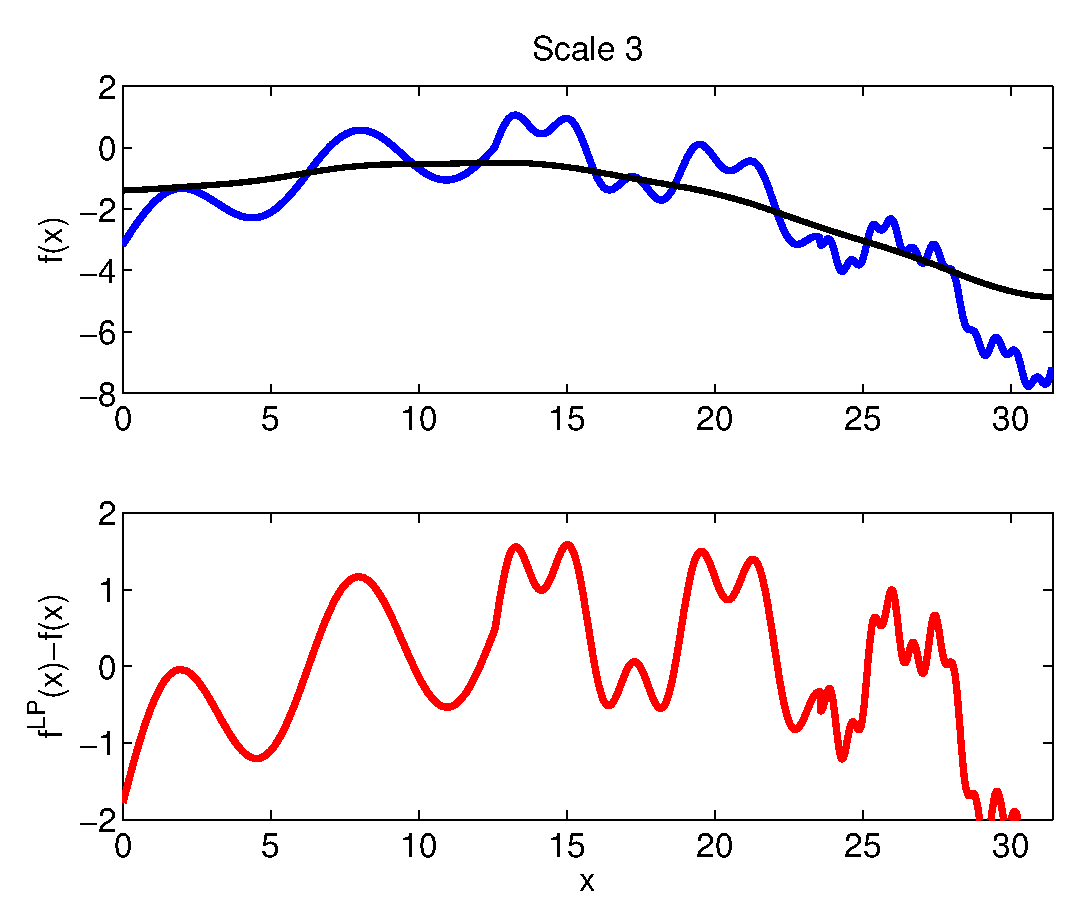
\includegraphics[width=\textwidth]{Scale3_S2}
\caption{}
\label{subfig:LP_ex1}
\end{subfigure}
\begin{subfigure}{0.22\textwidth}
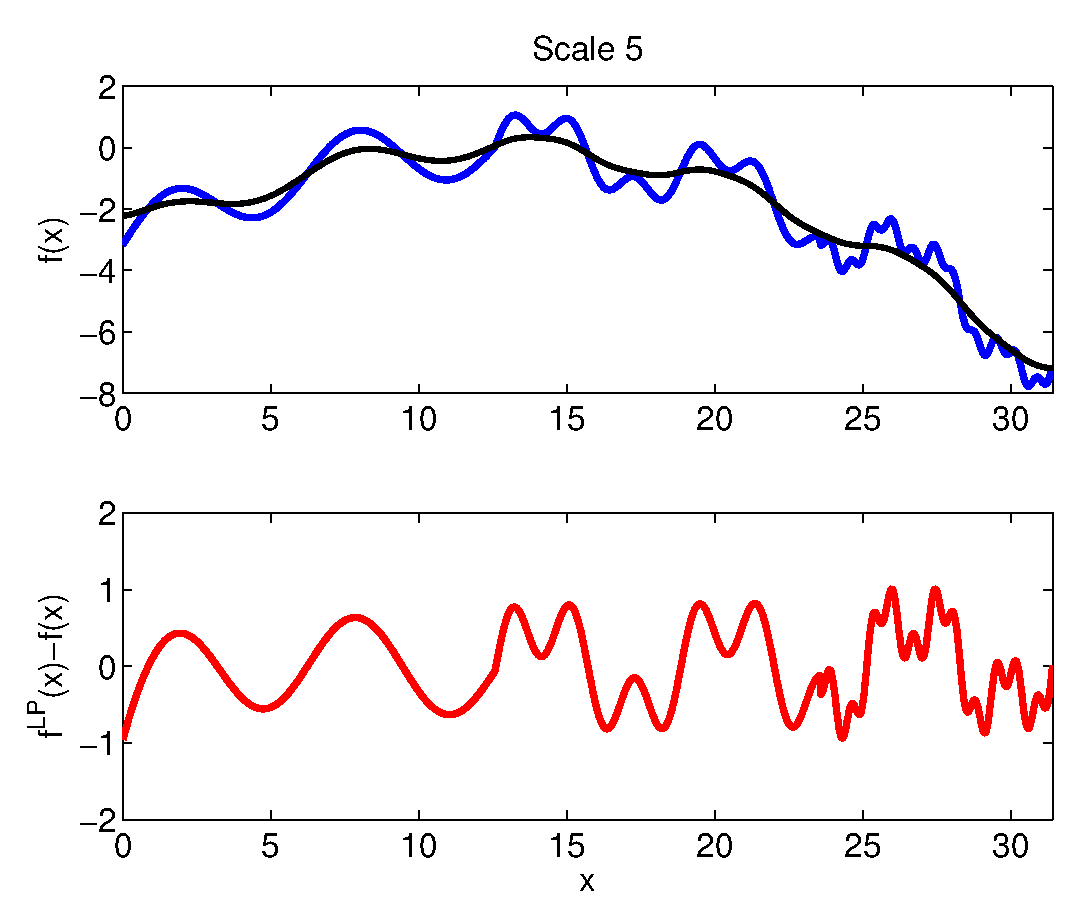
\includegraphics[width=\textwidth]{Scale5_S2}
\caption{}
\label{subfig:LP_ex2}
\end{subfigure}
\begin{subfigure}{0.22\textwidth}
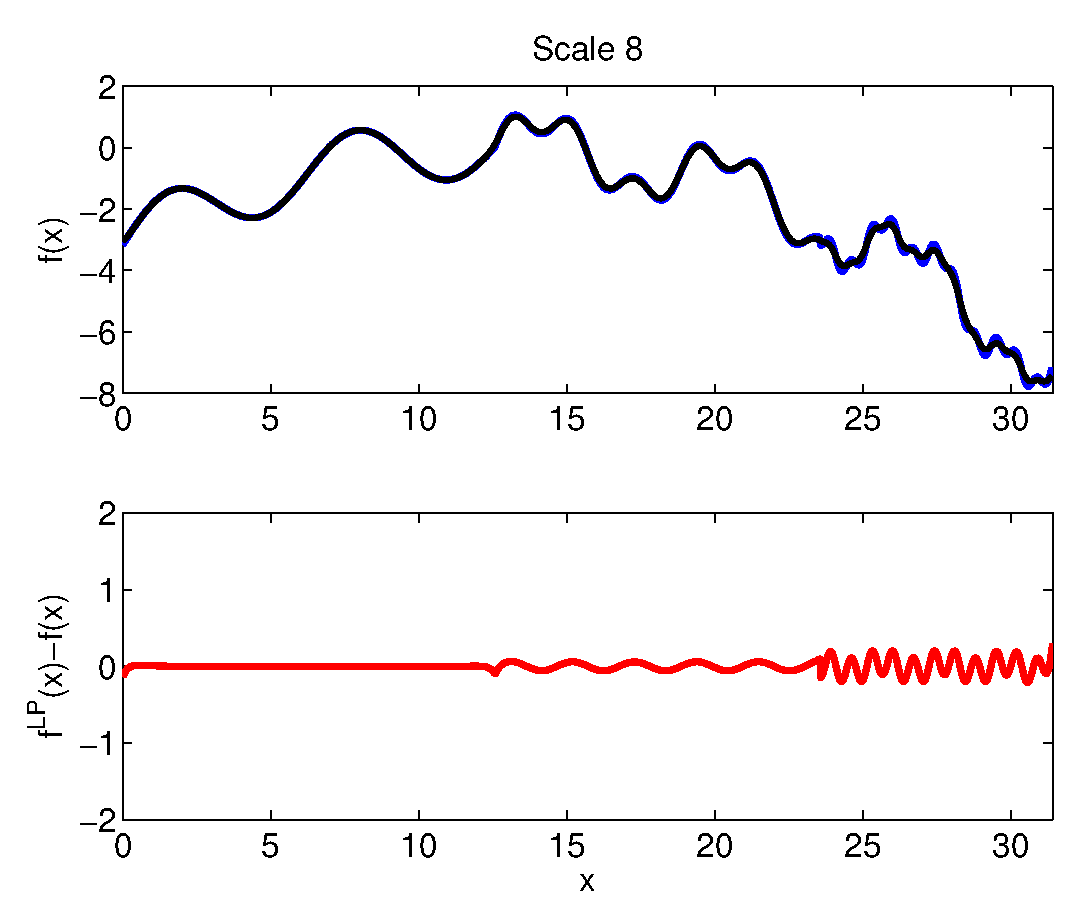
\includegraphics[width=\textwidth]{Scale8_S2}
\caption{}
\label{subfig:LP_ex3}
\end{subfigure}
\begin{subfigure}{0.22\textwidth}
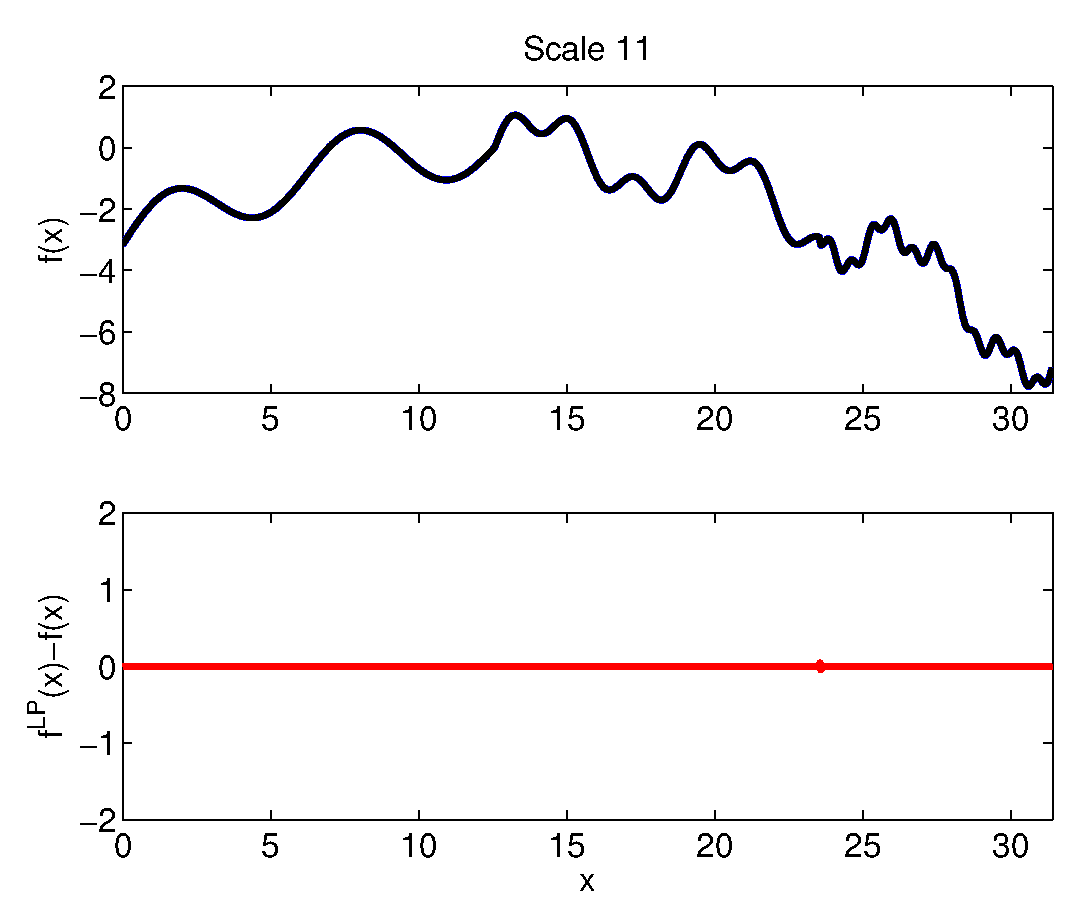
\includegraphics[width=\textwidth]{Scale11_S2}
\caption{}
\label{subfig:LP_ex4}
\end{subfigure}
\caption[Illustration of function approximation using Laplacian Pyramids at different scales]{Approximation of the function $\measfn(x)$ defined in \eqref{eq:LP_example} using Laplacian Pyramids for ``scales'' (\subref*{subfig:LP_ex1}) 3, (\subref*{subfig:LP_ex2}) 5, (\subref*{subfig:LP_ex3}) 8, and (\subref*{subfig:LP_ex4}) 11. The top shows the true function in blue and the LP approximation is shown in black, and the bottom shows the residual error in the LP approximation.}
\label{fig:LP_ex}
\end{figure}

\section{Models and Results} \label{sec:examples}

\subsection{A chemical reaction network}\label{subsec:rxn_network}

We first consider a chemical reaction network involving  multiple enzyme-substrate interactions \cite{zagaris2012stability}.
%
The reaction steps that comprise the network are\\
\begin{equation}
\begin{array}{rcl}
E + S \overset{e_1}{\underset{e_{-1}}{\leftrightharpoons}} & E:S & \overset{e_2}{\rightarrow} E + S^{*} \\
S + E \overset{b_1}{\underset{b_{-1}}{\leftrightharpoons}} & S:E & \overset{b_2}{\rightarrow} S + E^{*}\\
D + S^{*} \overset{d_1}{\underset{d_{-1}}{\leftrightharpoons}} & D:S^{*} & \overset{d_2}{\rightarrow} D + S\\
F + E^{*} \overset{f_1}{\underset{f_{-1}}{\leftrightharpoons}} & F:E^{*} & \overset{f_2}{\rightarrow} F + E
\end{array}
\end{equation}
The ``$^{*}$'' denotes an activated form of a species, and the ``:'' denotes a complex formed between two species; the complexes $E:S$ and $S:E$ are not equivalent.
%
There are 10 species in this reaction system.
%
However, one can write four conservation equations (since total $E$, $S$, $D$, and $F$ are all conserved) to reduce the system to 6 dimensions
(which we order as $S$, $E$, $E:S$, $S:E$, $D:S^{*}$, $F:E^{*}$).
%
We consider a parameter regime in which the ODE approximation of this scheme exhibits a separation of time scales, so that initial conditions quickly approach a two-dimensional manifold.
%
Details about the specific parameter values can be found in \app~\ref{app:merging}.

Although the dynamics of chemical reaction networks are typically described by a system of ODEs, the ODEs are only an approximation that holds
in the limit of a large number of molecules.
%
When the number of molecules is small, the system is inherently stochastic and its dynamics can be simulated using the
Gillespie Stochastic Simulation Algorithm (SSA) \cite{gillespie1977exact}; at intermediate molecule counts, the chemical Langevin approximation \cite{gillespie2000chemical}
becomes useful.
%
We can control the level of noise in our simulation by adjusting the volume $V$, and therefore, adjusting the number of molecules, in the system.
%
We take the volume small enough so that we can still observe appreciable stochasticity in small simulation bursts, but large enough (in our simulations, we take $V=10^5$) so that the underlying two-dimensional manifold is (relatively) smooth.

We generate 3000 initial conditions $\data_0(1), \dots, \data_0(3000) \in \mathbb{R}^6$ uniformly at random from the
region of state space where all concentrations (respecting conservation laws) are non-negative.
%
We evolve each point $\data_0(t)$ forward for 10 time units using the SSA to obtain a point $\data(t) \in \mathbb{R}^6$;
according to the time scales calculated from the linearized ODEs, 10 time units is sufficiently long for the initial points in the ODE system to converge to the two-dimensional manifold,
but not long enough for the points to converge to a one-dimensional curve or to the final steady state (see \app~\ref{app:merging} for more details).
%
In our stochastic simulations, the initial points appear to converge to an approximate two-dimensional manifold
(in expected value, see \fig~\ref{fig:rxn_manifolds}).
%
We consider $\mathcal{Y} = \{ \data(t): t=1, \dots, 3000 \}$ to be representative points ``on" this apparent two-dimensional manifold.
%
From each manifold point $\data \in \mathcal{Y}$, we run 20 short simulation ``bursts'', each for 0.2 time units.
%
We denote the endpoints from the short simulations as $\mathcal{Y}^{burst}(\data)$.

\begin{figure}[t]
\centering
\begin{subfigure}{0.45\textwidth}
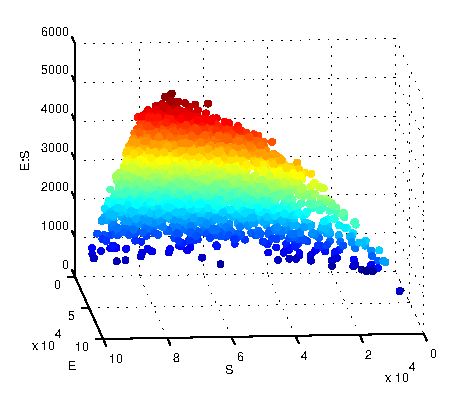
\includegraphics[height=5cm]{rxn_manifold1}\llap{\raisebox{4cm}{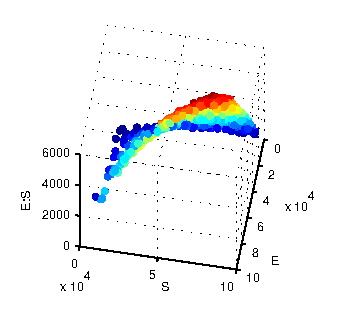
\includegraphics[height=2.25cm]{rxn_manifold1_2}}}
\caption{}
\label{subfig:rxn_manifolds1}
\end{subfigure}
\begin{subfigure}{0.45\textwidth}
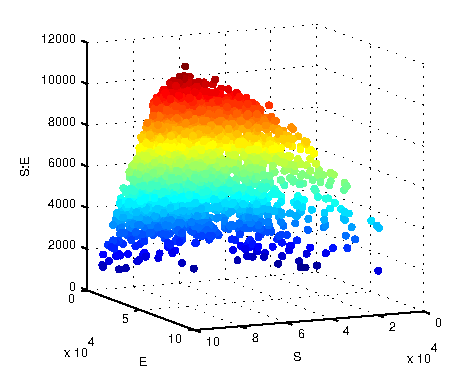
\includegraphics[height=5cm]{rxn_manifold2}\llap{\raisebox{4cm}{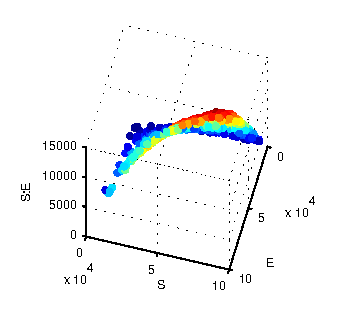
\includegraphics[height=2.25cm]{rxn_manifold2_2}}}
\caption{}
\label{subfig:rxn_manifolds2}
\end{subfigure}\\
\begin{subfigure}{0.45\textwidth}
\includegraphics[height=5cm]{rxn_manifold3}\llap{\raisebox{4cm}{\includegraphics[height=2.25cm]{rxn_manifold3_2}}}
\caption{}
\label{subfig:rxn_manifolds3}
\end{subfigure}
\begin{subfigure}{0.45\textwidth}
\includegraphics[height=5cm]{rxn_manifold4}\llap{\raisebox{4cm}{\includegraphics[height=2.25cm]{rxn_manifold4_2}}}
\caption{}
\label{subfig:rxn_manifolds4}
\end{subfigure}
\caption[Projections of chemical reaction network data]{Projections of the data obtained from stochastic simulation of the chemical reaction network described in \sec~\ref{subsec:rxn_network}. The insets show rotations of the projections to illustrate the approximate two-dimensionality of the ``slow manifold''.}
    \label{fig:rxn_manifolds}
\end{figure}

We consider two different data sets from our simulations.
%
Data set 1, denoted $\mathcal{Y}_1$, consists of $\data(1), \dots, \data(2000)$, restricted to components $S$, $E$, $S:E$, and $F:E^{*}$, i.e.,
$$\mathcal{Y}_1 = \left\{
\left( \begin{array}{cccccc}
1 & 0 & 0 & 0 & 0 & 0 \\
0 & 1 & 0 & 0 & 0 & 0 \\
0 & 0 & 0 & 1 & 0 & 0 \\
0 & 0 & 0 & 0 & 0 & 1
\end{array} \right) \data(t) \in \mathbb{R}^4: t=1, \dots, 2000 \right\}.$$
%
Data set 2, denoted $\mathcal{Y}_2$, consists of $\data(1500), \dots, \data(3000)$, restricted to components $S$, $E$, $E:S$, and $D:S^{*}$, i.e.,
$$\mathcal{Y}_2 = \left\{
\left( \begin{array}{cccccc}
1 & 0 & 0 & 0 & 0 & 0 \\
0 & 1 & 0 & 0 & 0 & 0 \\
0 & 0 & 1 & 0 & 0 & 0 \\
0 & 0 & 0 & 0 & 1 & 0
\end{array} \right)
\data(t) \in \mathbb{R}^4: t=1500, \dots, 3000 \right\}.$$
%
The endpoints of the simulation bursts for the two data sets, $\mathcal{Y}^{burst}_1(\data)$ and $\mathcal{Y}^{burst}_2(\data)$, are defined analogously.
%
We then estimate the covariances for each point in each data set as
\begin{equation}
\widehat{\mathbf{C}}_i(\data) = \sum_{\mathbf{z} \in \mathcal{Y}^{burst}_i(\data)} \left( \mathbf{z} - \hat{\mathbf{\mu}}_i(\data) \right)\left( \mathbf{z} - \hat{\mathbf{\mu}}_i(\data) \right)^T, \data \in \mathcal{Y}_i, i \in \{1, 2\}
\end{equation}
where $\hat{\mathbf{\mu}}_i(\data)$ is the empirical mean of $\mathcal{Y}^{burst}_i(\data)$.

We first demonstrate that NIV produces the same embeddings for $\mathcal{Y}_1$ and $\mathcal{Y}_2$, even though the two data sets contain information of different chemical species.
%
\fig~\ref{fig:rxn_embedding} shows the two-dimensional NIV embeddings for the two different data sets; the embeddings appear visually consistent.
%
We also note that both $\mathcal{Y}_1$ and $\mathcal{Y}_2$ contain points that are projections of $\data(1500), \dots, \data(2000)$.
%
We therefore compute the correlation between the embedding coordinates for these points common to $\mathcal{Y}_1$ and $\mathcal{Y}_2$.
%
We obtain a correlation of 0.97 and 0.95 for the first and second NIV, respectively, indicating that the two embeddings are in quantitative
agreement with each other.
%
We would like to note that both $\mathcal{Y}_1$ and $\mathcal{Y}_2$ are sufficiently high-dimensional (``rich enough'') to allows us to recover
the common underlying two-dimensional manifold.
%
\begin{figure}[t]
\centering
\begin{subfigure}{0.4\textwidth}
\includegraphics[width=\textwidth]{rxn_NLICA1}
\caption{}
\label{subfig:rxn_embedding1}
\end{subfigure}
\begin{subfigure}{0.4\textwidth}
\includegraphics[width=\textwidth]{rxn_NLICA2}
\caption{}
\label{subfig:rxn_embedding2}
\end{subfigure}\\
\begin{subfigure}{0.4\textwidth}
\includegraphics[width=\textwidth]{rxn_NLICA_corr1}
\caption{}
\label{subfig:rxn_corr1}
\end{subfigure}
\begin{subfigure}{0.4\textwidth}
\includegraphics[width=\textwidth]{rxn_NLICA_corr2}
\caption{}
\label{subfig:rxn_corr2}
\end{subfigure}
\caption[Intrinsic variable embeddings for chemical reaction network data]{(\subref*{subfig:rxn_embedding1}) NIV embedding obtained from $\mathcal{Y}_1$ (observations of components E, S, S:E, and F:E$^{*}$), colored by $S$. (\subref*{subfig:rxn_embedding2}) NIV embedding obtained from $\mathcal{Y}_2$ (observations of components E, S, E:S, and D:S$^{*}$), colored by $S$. Visually, we can see that the embeddings obtained from $\mathcal{Y}_1$ and $\mathcal{Y}_2$ are consistent, even though the two data sets consist of observations of different chemical species. (\subref*{subfig:rxn_corr1}) Correlation of first NIV between two different embeddings (correlation=0.97). (\subref*{subfig:rxn_corr2})  Correlation of second NIV between two different embeddings (correlation=0.95). We obtain a good quantitative agreement between the embedding coordinates for the two data sets.}
    \label{fig:rxn_embedding}
\end{figure}

To determine whether a sufficient amount of data is available to obtain an accurate embedding, we compute the NIV embeddings for different numbers of data points
(arising from different numbers of trajectories initialized randomly in the full concentration space).
%
\fig~\ref{fig:rxn_convergence} shows the two-dimensional NIV embeddings and corresponding eigenvalue spectra of the kernel for the Gillespie SSA example computed from 10, 100, 500, and 1500 data points.
%
We observe that the eigenvalue spectra appear converged for 100 data points and above.
%
This implies that a sufficient amount of data is available merely to discover the intrinsic variables.
%
However, we observe that 100 points are insufficient to construct a self-consistent embedding {\em in the two variables discovered}.
%
In order to account for the different scaling of the NIV coordinate axes, we require at least 500 data points.
%
This last convergence is exemplified in \fig~\ref{fig:rxn_convergence}\subref*{subfig:rxn_convergence3}, \subref*{subfig:rxn_convergence4}.
%
The convergence of the spectrum of the kernel and the ultimate self-consistency of the NIV embedding is our empirical indicator that a sufficient amount of data is available.
\begin{figure}[t]
\centering
\begin{subfigure}{0.22\textwidth}
\includegraphics[width=\textwidth]{rxn_npoints_embed1}
\includegraphics[width=\textwidth]{rxn_npoints_spectrum1}
\caption{}
\label{subfig:rxn_convergence1}
\end{subfigure}
\hfill
\begin{subfigure}{0.22\textwidth}
\includegraphics[width=\textwidth]{rxn_npoints_embed2}\\
\includegraphics[width=\textwidth]{rxn_npoints_spectrum2}
\caption{}
\label{subfig:rxn_convergence2}
\end{subfigure}
\hfill
\begin{subfigure}{0.22\textwidth}
\includegraphics[width=\textwidth]{rxn_npoints_embed4}\\
\includegraphics[width=\textwidth]{rxn_npoints_spectrum4}
\caption{}
\label{subfig:rxn_convergence3}
\end{subfigure}
\hfill
\begin{subfigure}{0.22\textwidth}
\includegraphics[width=\textwidth]{rxn_npoints_embed6}\\
\includegraphics[width=\textwidth]{rxn_npoints_spectrum6}
\caption{}
\label{subfig:rxn_convergence4}
\end{subfigure}
\caption[Convergence of intrinsic variable embeddings as a function of the number of data points]{Two-dimensional NIV embeddings (top) and corresponding eigenvalue spectra (bottom) calculated from subsets of $\mathcal{Y}_1$ containing (\subref*{subfig:rxn_convergence1}) 10 data points, (\subref*{subfig:rxn_convergence2}) 100 data points, (\subref*{subfig:rxn_convergence3}) 500 data points, and (\subref*{subfig:rxn_convergence4}) 1500 data points. One can see that the embedding and spectrum in \subref*{subfig:rxn_convergence1} is inconsistent with the other embeddings, and that, although the spectrum in \subref*{subfig:rxn_convergence2} appears converged, the embedding is not converged until \subref*{subfig:rxn_convergence3}. }
\label{fig:rxn_convergence}
\end{figure}

We then use NIV together with Laplacian Pyramids to estimate the values of $S:E$ and $F:E^{*}$ for $\mathcal{Y}_2$.
%
Because $\mathcal{Y}_1$ and $\mathcal{Y}_2$ are measured for different components, there is no simple way to estimate $S:E$ and $F:E^{*}$ directly in the observation space.
%
Instead, we must first embed the data into the NIV space so that we can compute neighbors {\em between the two data sets}.
%
We use $\mathcal{Y}_1$ to train an LP function from the two-dimensional NIV embedding to $S:E$ and $F:E^{*}$.
%
We then use this function to predict the values  of $S:E$ and $F:E^{*}$ for $\mathcal{Y}_2$, using the computed NIV embedding for $\mathcal{Y}_2$.
%
In this way, we are exploiting the fact that the NIV embedding is intrinsic and consistent between the two data sets, even though the two data sets contain measurements of different chemical species.

The results of the LP prediction are shown in \fig~\ref{fig:rxn_recon}.
%
The normalized mean-squared errors between the true and estimated values for $S:E$ and $F:E^{*}$, defined as $\frac{\langle (y_{true}-y_{pred})^2 \rangle}{\langle y_{true}^2 \rangle}$, are 0.0372 and 0.0287 , respectively.
%
Therefore, we can effectively estimate the unobserved components in the reaction network using NIV together with LP.
%

\begin{figure}[t]
\centering
\begin{subfigure}{0.4\textwidth}
\includegraphics[width=\textwidth]{rxn_recon4}
\caption{}
\label{subfig:rxn_recon1}
\end{subfigure}
\begin{subfigure}{0.4\textwidth}
\includegraphics[width=\textwidth]{rxn_recon6}
\caption{}
\label{subfig:rxn_recon2}
\end{subfigure}
    \caption[Laplacian Pyramids reconstructions for chemical reaction network data]{LP reconstructions of (\subref*{subfig:rxn_recon1}) $S:E$ and (\subref*{subfig:rxn_recon2}) $F:E^{*}$ for $\mathcal{Y}_2$, using $\mathcal{Y}_1$ as training data.}
    \label{fig:rxn_recon}
\end{figure}

\subsection{Alanine dipeptide}

Our second example comes from the molecular dynamics simulation of a small peptide fragment.
%
Alanine dipeptide (Ala2) is often used as a ``prototypical'' protein caricature for simulation studies
\cite{apostolakis1999calculation, bolhuis2000reaction, chekmarev2004long, ma2005automatic, frewen2009exploration, ferguson2011integrating}.
%
We simulate the motion of Ala2 in explicit solvent using the AMBER 10 molecular simulation package \cite{case2008Amber} with an
optimized version \cite{best2009optimized} of the AMBER ff03 force field \cite{duan2003point}.
%
The molecule is solvated with 638 TIP3P water molecules \cite{jorgensen1983comparison}
with periodic boundary conditions, and the particle mesh Ewald method is used for long-range electrostatic interactions \cite{essmann1995smooth}.
%
The simulation is performed at constant volume and temperature (NVT ensemble), with the temperature being maintained at 300~K with a Langevin thermostat \cite{loncharich1992langevin}.
%
Hydrogen bond lengths are fixed using the SHAKE algorithm \cite{ryckaert1977numerical}.
%
The two dihedral angles $\phi$ and $\psi$ are known to parameterize the free energy surface, which contains three important minima (labeled A, B, and C, see \fig~\ref{fig:ala_fes}\subref*{subfig:FES}).
%
Our simulations are concentrated around minimum B in the free energy surface, located at $\phi \approx -65^{\circ}$, $\psi \approx 150^{\circ}$.
%
We choose to sample only around minimum B, as each data set must sample the same region of the potential energy surface to obtain consistent NIV, as described in \sec~\ref{subsec:mahalanobis}.
%
We start many simulations at $10^{\circ}$ away from the minimum, and allow the simulations to each run for 0.1~ps, while recording the configuration of Ala2 every 1~fs (therefore, each trajectory is 100 points long).
%
Configurations are recorded with all atoms except the hydrogens.

\begin{figure}[t]
\centering
\begin{subfigure}{0.6\textwidth}
\includegraphics[width=\textwidth]{FES}
\caption{}
\label{subfig:FES}
\end{subfigure}
\begin{subfigure}{0.3\textwidth}
\includegraphics[width=\textwidth]{molecule_labeled2}
\caption{}
\label{subfig:ala_config}
\end{subfigure}
\caption[Alanine dipeptide free energy surface and representative molecular configuration]{(\subref*{subfig:FES}) Free energy surface for Ala2. The relevant minima are labeled A, B, and C, and the corresponding molecular configurations are shown.
(\subref*{subfig:ala_config}) Sample representative molecular structure of Ala2, excluding the hydrogens. The atoms are numbered and the two dihedral angles $\phi$ and $\psi$ are indicated.}
\label{fig:ala_fes}
\end{figure}


We first compare NIV with direct diffusion maps \cite{coifman2005geometric}, an established nonlinear dimensionality reduction technique.
%
We consider 10,000 data points from our simulation $\data(1), \dots, \data(10000) \in \mathbb{R}^{30}$; every 100 data points comes from a continuous simulation trajectory.
%
We construct two data sets:
%
$\mathcal{Y}_{even} = \{\data(t) \text{ restricted to atoms 2, 4, 6, 8, and 10}: t=1, \dots, 10000 \}$,
and $\mathcal{Y}_{odd} = \{\data(t) \text{ restricted to atoms 5, 7, and 9}: t=1, \dots, 10000 \}$ (see \fig~\ref{fig:ala_fes}\subref*{subfig:ala_config} for the atom indexing).
%
We then compute the NIV and diffusion maps embeddings for $\mathcal{Y}_{even}$ and $\mathcal{Y}_{odd}$;
for NIV, we compute the covariances as in \eqref{eq:cov1}, with $L=10$.

The correlation between the NIV coordinates for the two data sets and the diffusion map (DM) coordinates for the two data sets are shown in \fig~\ref{fig:ala_corr}.
%
The correlation between the two NIV embeddings is higher than the correlation between the two diffusion map embeddings.
Therefore, it appears advantageous to use NIV over diffusion maps if one wishes to obtain a consistent embedding and merge data sets from different observation domains (as long as the two main assumptions underpinning the NIV algorithm hold).

\begin{figure}[t]
\centering
\begin{subfigure}{0.4\textwidth}
\includegraphics[width=\textwidth]{NLICA_corr}
\caption{}
\label{subfig:ala_corr1}
\end{subfigure}
\begin{subfigure}{0.4\textwidth}
\includegraphics[width=\textwidth]{DM_corr}
\caption{}
\label{subfig:ala_corr2}
\end{subfigure}
\caption[Comparison of intrinsic variable and diffusion maps embeddings for alanine dipeptide data]{(\subref*{subfig:ala_corr1}) Correlation between the second NIV computed using the atoms 2, 4, 6, 8, and 10 ($\psi_2^{even}$) and the second NIV computed using atoms 5, 7, and 9 ($\psi_2^{odd}$).
    (\subref*{subfig:ala_corr2}) Correlation between the second DM computed using the atoms 2, 4, 6, 8, and 10 ($DM_2^{even}$) and the second DM computed using atoms 5, 7, and 9 ($DM_2^{odd}$).
    The correlations for the first (not shown) and second NIV coordinates are found to be 0.62 and 0.84, respectively.
    The correlations for the first (not shown) and second DM coordinates are found to be 0.54 and 0.60, respectively. }
    \label{fig:ala_corr}
\end{figure}

We then use NIV together with LP to predict the conformation of Ala2 when we only observe some of the atoms.
%
We have 20000 data points $\data(1), \dots, \data(20000)$, where every 100 data points come from one continuous simulation trajectory.
%
Our first data set (which will serve as our training data for LP), $\mathcal{Y}_{all}$,
consists of the first 10000 data points ($\mathcal{Y}_{all} = \{\data(t): t=1, \dots, 10000\}$).
%
Our second data set (which will serve as our test data), $\mathcal{Y}_{odd}$, consists of the last 12000 data points restricted to {\em only} the odd atoms
($\mathcal{Y}_{odd} = \{ \data(t) \text{ restricted to the odd atoms}: t = 8001, \dots, 20000\}$).
%
We compute the covariances as in \eqref{eq:cov1} with $L=15$.
%
We compute the NIV embedding for the training data $\mathcal{Y}_{all}$ and the test data $\mathcal{Y}_{odd}$; we then use LP interpolation from the training data to predict the location of all the atoms for each point in the test data.

The NIV embedding for the training data $\mathcal{Y}_{all}$ is shown in \fig~\ref{fig:ala_embed}.
%
The embedding is three-dimensional, and visual inspection reveals that each coordinate can be directly linked with one physical variable:
the first coordinate describes the flipping of atoms 1 and 3, the second coordinate describes the dihedral angle $\phi$, and the third coordinate describes the dihedral angle $\psi$.
%
We calculate the correlation between the embedding coordinates for the points in $\mathcal{Y}_{all}$ and $\mathcal{Y}_{odd}$
that come from the common simulation data points $\data(8001), \dots, \data(10000)$.
%
The embeddings for the two data sets are found to be fairly consistent, with correlations of 0.97, 0.72, 0.85 for the first, second, and third NIV, respectively.

\begin{figure}[t]
\centering
\begin{subfigure}{0.3\textwidth}
    \includegraphics[width=\textwidth]{ala2_embed1}
    \caption{}
    \label{subfig:ala_embed1}
\end{subfigure}
\begin{subfigure}{0.3\textwidth}
    \includegraphics[width=\textwidth]{ala2_embed2}
    \caption{}
    \label{subfig:ala_embed2}
\end{subfigure}
\begin{subfigure}{0.3\textwidth}
    \includegraphics[width=\textwidth]{ala2_embed3}
    \caption{}
    \label{subfig:ala_embed3}
\end{subfigure}
    \caption[Intrinsic variable embeddings for alanine dipeptide data]{The 3-dimensional NIV embedding for Ala2 computed using $\mathcal{Y}_{all}$, colored by (\subref*{subfig:ala_embed1}) the y-coordinate of the first atom, (\subref*{subfig:ala_embed2}) the dihedral angle $\phi$, and (\subref*{subfig:ala_embed3}) the dihedral angle $\psi$. Each embedding is rotated so that the correlation between the colors and the relevant NIV can easily be seen.}
    \label{fig:ala_embed}
\end{figure}


\fig~\ref{fig:ala_recon} shows the reconstructed position from partial observation versus true position for certain selected atoms.
%
The strong correlation between the true and reconstructed positions is easier to appreciate for
atoms that move substantially within the data set (such as atoms 1 and 3).
%
\fig~\ref{fig:ala_molecules} shows molecular structures for the true and reconstructed configurations for selected data points;
there is qualitative agreement between the true and reconstructed configurations.
%
The discrepancies between the true and reconstructed positions of atoms 9 and 10 (see \fig~\ref{fig:ala_fes}\subref*{subfig:ala_config} for atom indexing) for some of the molecular structures are not surprising.
%
From \fig~\ref{fig:ala_embed}, one can see that the first three NIV describe the flipping of atoms 1 and 3 and the dihedral angles $\phi$ and $\psi$.
%
However, atoms 9 and 10 do not participate in any of these physical quantities, and so there is little information about their positions contained in the first three NIV.
%
We suspect that using more NIV would result in a better description of atoms 9 and 10 and lead to more accurate structure reconstructions.

For a brief comparison of LP over other reconstruction techniques, we also reconstruct configurations from the
NIV components using simple nearest-neighbor interpolation.
%
The average reconstruction error, scaled by the average bond length within the molecule, is shown in \fig~\ref{fig:ala_mse};
LP arguably outperforms simple nearest neighbor search for all of the atoms.
%
To determine why LP outperforms nearest neighbor search, we examine the errors at different scales in the LP algorithm.
%
The example described in \fig~\ref{fig:LP_ex} demonstrates the appropriateness of the LP algorithm to signals with an intrinsic multiscale structure.
%
We perform a similar analysis using the data from the alanine dipeptide example, and show that the observed signal does exhibit a similar error structure,
with large errors in some regions of NIV space and small errors in other regions;
these results are shown in \fig~\ref{fig:LapPyr_ala2_errors}.
%
We therefore conclude that the alanine dipeptide data does contain a measure of multiscale behavior, and, therefore, that LP is an appropriate algorithm for reconstruction.

\begin{figure}[t]
  \centering
        \includegraphics[width=3.5in]{fig9}
  \caption[Laplacian Pyramids reconstruction for alanine dipeptide data]{The correlation between the true position and the reconstructed position (using LP) for the test data. The columns correspond the x-, y-, and z-coordinates, and the rows correspond to atoms 1, 2, 3, 6, and 8.}
  \label{fig:ala_recon}
\end{figure}

\begin{figure}[t]
\begin{subfigure}{0.3\textwidth}
\centering
\includegraphics[width=\textwidth,trim=0in 0.7in 0in 0in, clip]{molecule300_balls}
\includegraphics[width=\textwidth,trim=0in 0.7in 0in 0in, clip]{molecule300_wire}
\caption{}
\label{subfig:ala_molecules1}
\end{subfigure}
%
\hfill
%
\begin{subfigure}{0.3\textwidth}
\centering
\includegraphics[width=\textwidth,trim=0in 0.7in 0in 0in, clip]{molecule600_balls}
\includegraphics[width=\textwidth,trim=0in 0.7in 0in 0in, clip]{molecule600_wire}
\caption{}
\label{subfig:ala_molecules2}
\end{subfigure}
%
\hfill
%
\begin{subfigure}{0.3\textwidth}
\centering
\includegraphics[width=\textwidth,trim=0in 0.7in 0in 0in, clip]{molecule900_balls}
\includegraphics[width=\textwidth,trim=0in 0.7in 0in 0in, clip]{molecule900_wire}
\caption{}
\label{subfig:ala_molecules3}
\end{subfigure}
    \caption[Example reconstructed alanine dipeptide configurations]{True structure (black) and reconstructed structure (red) for three different data points. Each data point is shown in ``ball-and-stick'' representation (left) and ``wireframe'' representation (right) so that the discrepancies can easily be seen between the different configurations.}
    \label{fig:ala_molecules}
\end{figure}

\begin{figure}[t]
	\centering
    \includegraphics[width=3in]{fig11}
    \caption[Average error in reconstructed alanine dipeptide configurations]{Mean squared error of reconstructed position, normalized by the average bond length, for each atom in Ala2.
    The positions were reconstructed using both LP and nearest neighbor (nn) interpolation.}
    \label{fig:ala_mse}
\end{figure}

\begin{figure}[t]
    \centering
    \includegraphics[width=3in]{fig10b}
    \caption[Error in selected coordinate of reconstructed alanine dipeptide configurations]{The error in the reconstructed position of the z-coordinate of atom 10 as a function of $\psi_1$. One can see that the error is large when $\psi_1$ is large (similar to the error structure in \fig~\ref{fig:LP_ex}), demonstrating that our data is indeed multiscale and that Laplacian Pyramids is an appropriate interpolation algorithm to use.}
    \label{fig:LapPyr_ala2_errors}
\end{figure}

\section{Discussion} \label{sec:conclusions}
%
We have used Nonlinear Intrinsic Variables to analyze two complex atomistic simulations: a stochastic simulation of a chemical reaction network and a molecular dynamics simulation of alanine dipeptide.
%
In both examples, we were able to uncover the intrinsic variables governing the underlying stochastic process, which are independent
of the particular measurement or observation  of the system (under the conditions mentioned).
%
The uniqueness of the embedding coordinates allowed us to compare and merge data sets from different measurement functions,
and therefore allowed us to use an interpolation/extension scheme (here Laplacian Pyramids) to complete partial observations.
%
Different interpolation techniques (e.g. kriging \cite{matheron1963principles, matheron1973intrinsic}, geometric harmonics \cite{coifman2006geometric},  versions of the Nystr\"{o}m extension) can and should
be explored, since the performance of such techniques may well be problem dependent, especially for multiscale, complex simulation data.

There are many open questions leading to interesting research directions to be explored.
%
In this work, we considered data sets that consist of different partial observations, but in which each data set samples the entire underlying manifold in
what we loosely referred to as a ``representative enough" way.
%
However, NIV could also be used to merge data sets when each data set samples only a portion of the manifold, provided there is enough overlap to ``register'' the embeddings.
%
Merging data sets that come from different portions of the manifold would not only require scaling the embedding coordinates,
but also shifting and possibly permuting the embedding coordinates (in this spirit, see the discussion in Lafon {\em et al.} \cite{lafon2006data}).
%
The ability to merge data from different regions would then allow us to analyze systems where complete sampling is computationally intractable,
such as molecular systems with several high energy barriers separating regions of state space.

Other issues, such as accurately estimating the covariance matrices required for the computation of the Mahalanobis distance, are also of current research interest.
%
It is clearly necessary to link this type of calculation with modern estimation techniques for (multiscale) diffusions \cite{ait2002maximum, ait2003effects, ait2008closed}
to test the appropriateness of the window sampling lengths selected; this will determine the accuracy of the noise covariance estimation by eliminating
the bias due to drift variations.
%
We are confident that the exploration of these open questions will enable the use of our methodology in many interesting applications, such as merging data from molecular simulations at different levels of granularity, or merging simulation data with experimental observations.

We have described using the Mahalanobis distance with diffusion maps to analyze two different types of data common in dynamical systems: data exhibiting dynamics on multiple time scales, and data obtained via several measurement/observation functions.
%
In the next chapter, we will address a third type of data (imaging data).
%
In this work, we will not be interested in removing the effects of fast variables or measurement functions, but instead factoring out rotational symmetries which arise from the experimental imaging setup.
%
We will present an extension of diffusion maps which allows us to simultaneously factor out symmetries and uncover patterns and structure in the imaging data set.
%
%For this particular example, recovering structure in the data set will correspond to ordering the images in order to recover the relevant developmental dynamics.




\chapter{Temporal Ordering of Images \label{ch:drosophila}}

\graphicspath{{ch-drosophila/figures/}}

{\em This work was published in \citep{dsilva2015temporal}}

\section{Introduction}

\begin{figure}[t]
\includegraphics{fig1}
\caption[Caricature illustrating the tasks of image registration and temporal ordering]{Caricature illustrating the tasks of image registration and temporal ordering. (A) Images of ``samples'', each in a different orientation and a different stage of development. (B) Registered and ordered samples. For this caricature, the registration and ordering is straightforward because the data set is small, the landmarks are visually apparent, and the developmental changes are easy to recognize.}
\label{fig:fish}
\end{figure}

In one of the common approaches to studies of developmental dynamics, a group of embryos is fixed and stained to visualize a particular biochemical or morphological process within a developing tissue.
%
The developmental dynamics must then be reconstructed from multiple embryos, each of which contributes only a snapshot of the relevant process along its developmental trajectory \citep{jaeger2004dynamic, peter2011gene, fowlkes2008quantitative}.
%
Importantly, the ``age'' of any given embryo arrested in its development is often only approximately known.
%
Typically, what is known is
a certain time window to which a collection of embryos belongs \citep{ng2012large, richardson2014emage, castro2009automatic}.
%
Furthermore, images are often collected in different spatial orientations.
%
In order to recover the developmental dynamics from such data sets, snapshots of different embryos must first be spatially aligned or {\em registered}, and then ordered in time.


Temporal ordering and registration of images can be done manually
when the number of images is small and the differences between them are visually apparent.
%
\fig~\ref{fig:fish} shows a caricature of fish development which illustrates the processes of growth and patterning.
%
In this case, temporal ordering can be accomplished by arranging the fish by size, which is monotonic with the developmental progress.
%
Image registration is based on obvious morphological landmarks, such as the positions of the head and the fins.
%
In contrast to this example, real data pose nontrivial challenges for both registration and temporal ordering.
%
In general, the landmarks needed for registration, as well as the attributes which can be used to order the data, are not known {\it a priori}.
%
Additional challenges arise from embryo-to-embryo variability, sample size, and measurement noise.

We present a robust algorithmic approach to simultaneous registration and temporal ordering.
%
In contrast to a number of previous methodologies \citep{zitova2003image, rowley1998rotation, hajnal2010medical, greenspan1994rotation, zhao2003face, dubuis2013accurate}, our methodology does not rely on the {\em a priori} knowledge of landmarks for registration or markers of developmental progression.
%
The approach is based on vector diffusion maps \citep{singer2012vector}, a manifold learning algorithm which simultaneously addresses the problems of registration and temporal ordering.
%
This algorithm is one of several nonlinear dimensionality reduction techniques that have been developed over the past decade \citep{Belkin2003, coifman2005geometric, coifman2006geometric, tenenbaum2000global, roweis2000nonlinear}, for
applications ranging from analysis of cryo-electron microscopy (cryo-EM) images of individual molecules  \citep{zhao2014rotationally, singer2011viewing} to face recognition \citep{lafon2006data} and classification of CT scans \citep{fernandez2014diffusion}.

Here, the vector diffusion maps algorithm is adapted for the analysis of images of developing tissues in studies of developmental dynamics, with the main objective of revealing stereotypic developmental trajectories from fixed images.
%
To illustrate our approach, we analyze four experimental data sets.
%
Our first two data sets come from live imaging studies of {\em Drosophila} and zebrafish embryogenesis.
%
In both of these examples, the correct rotational orientation and temporal order are independently known, and these data sets will be used to validate our approach.
%
Our third data set consists of images from fixed {\em Drosophila} embryos where the correct orientation and order is unknown; here, we will show how the algorithm can help uncover developmental dynamics which are not readily apparent.
%
Our final data set consists of z-stacks of {\em Drosophila} wing discs, which we will use to illustrate how our methods can be used to analyze specific types of three-dimensional imaging data.
%
We also show how to compute an average trajectory from a set of registered and ordered fixed images to remove noise due to intersample variability and obtain a smooth description of the underlying developmental dynamics.

\section{Results}

\subsection{Vector diffusion maps for registration and temporal ordering}

Vector diffusion maps \citep{singer2012vector} is a manifold learning
technique developed for data sets which contain two sources of variability:
geometric symmetries, such as rotations of the images, which one would like to factor out,
and ``additional" directions of variability, such as temporal dynamics, which one would like to uncover.
%
Vector diffusion maps combine two algorithms, {\em angular synchronization} \citep{singer2011angular} for image registration and {\em diffusion maps} \citep{coifman2005geometric} for extracting intrinsic low-dimensional structure in data, into a single computation.
%
We will use the algorithm to register images of developing tissues with respect to planar rotations, as well as uncover the main direction of variability {\it after} removing rotational symmetries.
%
Although in general, images may contain variations due to rotations, translations, and scaling, we will remove the relevant translations and/or scaling via relatively simple image preprocessing, and focus only on factoring out rotations using the vector diffusion maps algorithm.
%
In the case that {\em all} relevant symmetries can be removed with straightforward preprocessing, our algorithms can extract the main direction of variability within the imaging data set.
%
We assume that this main direction of remaining variability in these images is parameterized by the developmental time of each embryo.
%
As a consequence, uncovering this direction should reveal the underlying dynamics.

\begin{figure}[t]
\includegraphics{fig2}
\caption[Schematic illustrating angular synchronization and diffusion maps]{Schematic illustrating angular synchronization and diffusion maps. (A) Set of vectors, each in a different orientation. The pairwise alignment angles are indicated. (B) The vectors from A, each rotated about their midpoint so that the set is globally aligned. Note that the chosen rotation angles are consistent with the pairwise alignments in A: the difference between a pair of angles in B is the same as the pairwise angle in A. (C) Data points (in black) which lie on a one-dimensional nonlinear curve in two dimensions. Each pair of points is connected by an edge, and the edge weight is related to the Euclidean distance between the points through a Gaussian kernel (see \SI), so that pairs of data point which are close are connected by darker (``stronger'') edges. (D) The data in C, colored by the first (non-trivial) eigenvector from the diffusion map computational procedure. The color intensity is monotonic with the perceived curve arclength, thus parametrizing the curve.}
\label{fig:schematics}
\end{figure}

Angular synchronization uses pairwise alignment information to register a set of images in a globally consistent way.
%
A schematic illustration of angular synchronization is shown in \fig~\ref{fig:schematics}A, where each image is represented as a vector, and the goal is to align the entire set of vectors given pairwise alignment measurements.
%
We first compute the angles needed to align pairs of vectors (or images), which in general requires no notion of a template function \citep{ahuja2007template, sonday2013noisy}.
%
In this work, we aligned pairs of images with respect to rotations by exhaustively searching over a discretized space of rotation angles to minimize the Euclidean distance between the pixels.
%
However, pairwise alignments can also be computed by aligning appropriate image landmarks or features \citep{ian1998statistical}.
%
When the data are noisy, these pairwise measurements may be inaccurate, and so we utilize {\em all} pairwise measurements to align the set of images robustly.
%
Using the alignment angles between all pairs of vectors, angular synchronization finds the set of rotation angles (one angle for each vector) that is most consistent with {\it all} pairwise measurements (see \SI); this is illustrated in \fig~\ref{fig:schematics}B.
%
In this schematic, registration via angular synchronization is trivial, as the pairwise measurements contain no noise.
%
However, the algorithm can register data sets even when many of the pairwise measurements are inaccurate \citep{singer2011angular}.

After removing variability due to rotations, the developmental dynamics may be revealed by ordering the data along the one-dimensional curve that parameterizes most of the remaining variability in the data.
%
Such a curve can be discovered using diffusion maps \citep{coifman2005geometric}, a nonlinear dimensionality reduction technique that reveals a parametrization of data that lies on a low-dimensional manifold in high-dimensional space.
%
The idea is illustrated in \fig~\ref{fig:schematics}C, where the data are two-dimensional points which lie on a one-dimensional (nonlinear) curve.
%
We use {\it local} information about the data to find a parametrization which respects the underlying manifold geometry, so that points which are close in high-dimensional space (e.g., images which look similar) are close in our parametrization.
%
This idea of locality is denoted by the color of the edges in \fig~\ref{fig:schematics}C:
data points which are close are connected by dark edges, and clearly, the dark edges are more ``informative" about the low-dimensional structure of the data.
%
The color in \fig~\ref{fig:schematics}D depicts the one-dimensional parametrization or ordering of the data that we can detect visually.
%
A detailed example of using vector diffusion maps to register and order synthetic data is given in \fig~\ref{fig:1d_demo}, and a step-by-step tutorial of the diffusion maps implementation is included in the \SI.
%
In our working examples, each data point will be of much higher dimension (e.g., a pixelated image or three-dimensional voxel data), and so we cannot extract this low-dimensional structure visually.
%
Instead, we will use diffusion maps which automatically uncovers a parametrization of our high-dimensional data from the eigenvectors of the appropriate matrix (see \SI).
%
Furthermore, the corresponding eigenvalues will allow us to test our assumption that our data approximately lie on a one-dimensional manifold (see \fig~\ref{fig:eigenvalues_drosophila_live}--\ref{fig:eigenvalues_wing_disc}).


\subsection{Method validation using live imaging}

\subsubsection{{\em Drosophila} gastrulation}

\begin{figure}[t]
\includegraphics{fig3}
\caption[Method validation using live imaging of \textit{Drosophila} embryos]{Method validation using live imaging of \textit{Drosophila} embryos. (A) Selected images from a live imaging study of a \textit{Drosophila} embryo during gastrulation. Scale bar indicates 50$\mu$m. Each frame is in an arbitrary rotational orientation, and the order of the frames has been shuffled. (B) Images from A registered and ordered by vector diffusion maps. The dorsal side of each embryo now appears at the top of each image, and the ventral side appears at the bottom. (C) The correlation between the recovered rotation angle (using vector diffusion maps) and the true rotation angle. The average absolute error in the recovered angles is $8.37 ^\circ$. (D) The correlation between the recovered rank (using vector diffusion maps) and the true rank. The rank correlation coefficient is $0.9989$. (E) The average error in the recovered angle and the rank correlation coefficient for $5$ independent live imaging studies. }
\label{fig:drosophila_live_imaging}
\end{figure}

To validate the proposed approach, we first applied our algorithm to a data set where the true temporal order and rotational orientation of the images were known {\em a priori}.
%
This data set was obtained through live imaging near the posterior pole of a vertically oriented {\it Drosophila} embryo during the twenty minutes spanning the late stages of cellularization through early gastrulation.
%
During this time window, the ventral furrow is formed, where the ventral side buckles towards the center of the embryo, internalizing the future muscle cells and forming a characteristic ``omega'' shape.
%
Germband extension then causes cells from the ventral side to move towards the posterior pole of the embryo, and then wrap around to the dorsal side \citep{leptin2005gastrulation}.
%
At the end of this process, cells which were originally on the ventral and posterior side of the embryo find themselves on the dorsal side, causing a similar ``omega'' to appear on the dorsal side.

\fig~\ref{fig:drosophila_live_imaging}A shows selected images from this live imaging data set, which contains $40$ consecutive frames taken at $30$~second time intervals at a fixed position within a single embryo.
%
Each image shows an optical cross-section near the posterior pole of a vertically oriented developing embryo, with the nuclei labeled by Histone-RFP.
%
Each frame was arbitrarily rotated, and the order of the frames was scrambled.
%
The task is now to register these images and order them in time to reconstruct the developmental trajectory.

We used vector diffusion maps to register and order the images.
%
\fig~\ref{fig:drosophila_live_imaging}B shows the images from \fig~\ref{fig:drosophila_live_imaging}A, now registered and ordered; the real time for each frame is also indicated.
%
With a small number of exceptions, the recovered ordering is consistent with the real time dynamics.
%
\fig~\ref{fig:drosophila_live_imaging}C and \fig~\ref{fig:drosophila_live_imaging}D  show the correlations between the recovered and true angles and rank orders, respectively, for the entire data set.
%
Both the angles and the ranks are recovered with a high degree of accuracy.
%
We note that determining which end of the trajectory corresponds to early in the developmental progression is a post-processing task that requires some {\em a priori} information. 

To assess the robustness of the proposed methodology, we repeated this procedure with four additional data sets extracted from independent live imaging studies spanning the same developmental time period.
%
The results are shown in \fig~\ref{fig:drosophila_live_imaging}E.
%
The errors in the recovered angles are all less than 10$^\circ$, and the rank correlation coefficients are consistently greater than 95\%, indicating that our methodology can reproducibly order data of this type.


\subsubsection{Zebrafish epiboly}

\begin{figure}[t]
\includegraphics{fig4}
\caption[Method validation using live imaging of a zebrafish embryo]{Method validation using live imaging of a zebrafish embryo. (A) Selected images from a movie of zebrafish epiboly. Scale bar indicates 200$\mu$m. Each frame is in an arbitrary rotational orientation, and the order of the frames has been shuffled. (B) Images from A after registration and ordering using vector diffusion maps. The real time of each frame is also indicated. (C) Correlation between the rank recovered using vector diffusion maps and the true rank.  The rank correlation coefficient is $0.9954$. The larger errors in the recovered ranks towards the beginning of the trajectory are due to the slow cell movement within that time window. }
\label{fig:zebrafish}
\end{figure}

As another validation for the proposed methodology, we applied our algorithm to a time-lapse movie  of zebrafish embryogenesis.
%
We used a publicly available live imaging data of zebrafish embryogenesis (\texttt{https://zfin.org/zf\_info/movies/Zebrafish.mov}) \cite{karlstrom1996flipbook}.
%
Taken with a differential interference contrast (DIC) microscope, the movie records the first $17$~hours of zebrafish development, from a single cell stage to a 16-somite stage.
%
We selected $120$ consecutive frames from this movie which capture 5.5~hours of epiboly (3.5--9~hours after fertilization).
%
In this experiment, embryos were immobilized for imaging so that the position and orientation remained fixed \citep{kane1996zebrafish}.
%
At the start of the time window, cells have divided 10--11 times and are accumulated in a cell mass above the yolk.
%
The cell mass is then compressed and the animal-vegetal axis of the embryo (vertical axis in \fig~\ref{fig:zebrafish}) shortens to form a spherical embryo shape by the end of the fourth hour of development.
%
Then, the yolk syncytial layer, which forms the boundary between the yolk and the cell mass, moves upward, forming a dome-shaped structure.
%
During this stage, the cells rearrange to form a uniform layer about four cells thick.
%
With time, this cell layer then spreads over across the yolk and expands toward the vegetal pole.
%
At the end of epiboly, the blastoderm completely engulfs the yolk.

As in the example of {\em Drosophila} embryo live imaging, the two-dimensional frames were randomly rotated and shuffled (\fig~\ref{fig:zebrafish}A).
%
We then used vector diffusion maps to register and order the frames.
%
The results are shown in \fig~\ref{fig:zebrafish}B.
%
The recovered rotations and order are consistent with the expected developmental dynamics, as shown in the correlations between the recovered and true ranks (\fig~\ref{fig:zebrafish}C).
%
Quantitatively, the rank correlation coefficient for this data set is 0.9954, and the average error in the recovered angle is $4.14^\circ$.
%
Some errors in ordering images of the early embryo result from slow cell movement during the early developmental stage where cells divide and accumulate above the yolk.
%
During epiboly, cell movement is more dynamic and the recovered ordering is more consistent with the real dynamics.

In summary, we have shown that our approach to temporal ordering performs very well on imaging data of two different developmental processes ({\em Drosophila} gastrulation and zebrafish epiboly), taken with two different imaging methods (fluorescent microscopy and DIC) where the true temporal order is known {\em a priori}.
%
Provided there exist significant dynamics within the data set and that the developmental trajectory is well-sampled, the developmental dynamics can be recovered.

\subsection{Data sets with intersample variability}

\subsubsection{Fixed images of {\em Drosophila} gastrulation}


We have analyzed how our algorithm performs on two model data sets where all images come from a single embryo.
%
In practice, we are interested in cases where each image comes from a different embryo, and the largest source of noise in the considered data set arises from embryo-to-embryo variability.
%
To demonstrate that our methods are robust to such variations,
we constructed a synthetic time course data set by selecting a random image from one of five {\em Drosophila} live imaging data sets (those data sets used in \fig~\ref{fig:drosophila_live_imaging}) at each time point.
%
The resulting data set is spatially unregistered, scrambled in time, and reflects embryo-to-embryo variability.
%
The median rank correlation coefficient when ordering such a synthetic time course using our methodology was 0.77, indicating that the algorithm can recover the temporal order even under noisy conditions.

We then applied our approach to a data set where the true rotational orientation and temporal order was not known {\it a priori}.
%
\fig~\ref{fig:drosophila_fixed_images}A shows selected images from a set of $120$ images of developing {\em Drosophila} embryos which cover a thirty minute time interval spanning late cellularization through gastrulation.
%
This data set is more complex than the live imaging data sets in that it contains significantly more images, each of which provides information about tissue morphology and the spatial distribution of two regulatory proteins.
%
Each image shows an optical cross-section of the posterior view of a {\em different} embryo at a different rotational orientation and fixed at a different (and unknown) developmental time.
%
The nuclei (gray) were labeled with DAPI, a DNA stain.
%
Embryos were stained with the antibody that recognizes Twist (Twi, shown in green), a transcription factor which specifies the cells of the future muscle tissue.
%
Another signal is provided by the phosphorylated form of the extracellular signal regulated kinase (dpERK, shown in red), an enzyme that, in this context, specifies a subset of neuronal cells \citep{Lim2013kinetics}.

\fig~\ref{fig:drosophila_fixed_images}B shows the selected images in \fig~\ref{fig:drosophila_fixed_images}A, now registered and ordered using vector diffusion maps.
%
Registered and ordered images of individual embryos can then be used to construct a representative average trajectory. 
%
Each snapshot in the average trajectory is the (weighted) average of a group of successive images from the registered and ordered data set (see \SI).
%
Averaging successive images removes some of the interembryo variability, so that sequential snapshots of this averaged trajectory, shown in \fig~\ref{fig:drosophila_fixed_images}C, serve as a summary of the stereotypic developmental dynamics.

\begin{figure}[t]
\includegraphics{fig5}
\caption[Analysis of images of fixed \textit{Drosophila} embryos]{Analysis of images of fixed \textit{Drosophila} embryos. {(A)} Images of \textit{ Drosophila} embryos, stained for nuclei (gray), Twi (green), and dpERK (red). Scale bar indicates approximately 50$\mu$m (images have been rescaled to remove slight interembryo size variations).  Each image is of a different embryo arrested at a different developmental time and in a different rotational orientation. {(B)} Data from {\it A}, registered and ordered using vector diffusion maps. The expert rank for each image is indicated. {(C)} A representative ``developmental trajectory'' obtained from local averaging of the entire set of registered and ordered images (see \SI). {(D)} Correlation between the image ranks calculated from the vector diffusion maps algorithm and the ranks obtained from ordering by an expert. The rank correlation coefficient is $0.9716$. }
\label{fig:drosophila_fixed_images}
\end{figure}


From this average trajectory, we can now easily see the developmental progression consistent with the known dynamics:
%
dpERK first appears as two lateral peaks at the ventrolateral side of the embryo, and a third dpERK peak then appears at the dorsal side of the embryo.
%
During mesoderm invagination, the two ventrolateral dpERK peaks merge together, eventually forming, together with Twi, the ``omega'' shape.
%
The dorsal dpERK peak then disappears during germband extension as cells from the ventral side wrap around to the dorsal side.
%
At the end of this process, similar ``omegas'' formed by Twi and dpERK appear on the dorsal side of the embryo; these patterns are most readily seen in the last image of \fig~\ref{fig:drosophila_fixed_images}C.
%
Thus, vector diffusion maps can accomplish the tasks presented in the caricature in \fig~\ref{fig:fish}, even in the absence of information about image landmarks and without {\it a priori} knowledge of developmental features.

To evaluate the quality of our registration and ordering, we can use prior knowledge about the developmental system.
%
The Twi signal is known to form a single peak at the ventralmost point of the embryo.
%
We found that the standard deviation in the location of this peak in the set of registered images was $\sim$8$^\circ$,
indicating that the algorithm successfully aligns the ventralmost points of the images.
%
Because the developmental time of each embryo cannot be easily estimated, we have few options for evaluating the quality of our temporal ordering.
%
We compared the ordering obtained from vector diffusion maps to the ordering provided by a trained embryologist who is knowledgeable about the developmental progression and the important image features.
%
The ranks from the ordering provided by the embryologist, which we will refer to as the ``expert rank'', are indicated for the images in \fig~\ref{fig:drosophila_fixed_images}B , and the rank correlation (see \fig~\ref{fig:drosophila_fixed_images}D) shows that our ordering is consistent with the expert ordering.


\subsubsection{Fixed z-stacks of {\em Drosophila} wing discs}

\begin{figure}[t]
\includegraphics{fig6}
\caption[Analysis of three-dimensional {\em Drosophila} wing disc z-stacks]{Analysis of three-dimensional {\em Drosophila} wing disc z-stacks. (A) Maximum projections of an example three-dimensional {\em Drosophila} wing disc z-stack. The anterior-posterior (A-P) and dorsal-ventral (D-V) axes are indicated. Discs express the Dad-GFP reporter construct (green), and are stained for Spalt (red), Wingless (gray), and Patched (gray). Projections along the $x$-, $y$-, and $z$-axes are shown. (B) Example three-dimensional images, ordered using diffusion maps. The time cohort, as assessed by an expert, is indicated for each image, and the rank correlation coefficient between the diffusion maps ordering and the expert timing is 0.9427. (C) The average developmental trajectory for the registered and ordered images. }
\label{fig:wing_disc}
\end{figure}

In this section we show that the approach can readily be applied to three-dimensional data. 
%
We restrict ourselves to the case where an obvious fixed axis exists, so that only rotations of the three-dimensional data around this axis need be taken into account.  
%
This does not constitute an inherent limitation for vector diffusion maps. 
%
While for simplicity here we will not discuss the general  case, incorporating general 3D symmetries is possible \citep{arie2012global, wang2013exact, cucuringu2012eigenvector}. 

To demonstrate this approach, we used an existing three-dimensional data set of fixed {\em Drosophila} wing imaginal discs \citep{hamaratoglu2011dpp}.
%
Imaginal discs are groups of progenitor cells in fly larva that will transform into specific organs during metamorphosis.
%
The wing disc is an imaginal disc that gives rise to the wing, thorax, and hinge.
%
The data set is composed of 46 fixed wing discs whose developmental times range from 72 to 112~hours after fertilization.
%
Each disc contains 21 z-slices taken at 1~$\mu$m intervals.
%
The discs were dissected from larvae expressing the Dad-GFP reporter construct (green) and stained with antibodies that recognize Spalt (red), Wingless (gray), and Patched (gray), the factors that play important roles in disc patterning and growth (\fig~\ref{fig:wing_disc}A).

In the wing disc, the anterior-posterior and dorsal-ventral axes are significantly larger than the third principal axis (see \fig~\ref{fig:wing_disc}A). 
%
Therefore, we need not consider registration in all three dimensions, and can instead focus on registering the wing discs with respect to rotations only in the x-y plane.
%
To register the data, we first aligned the maximum intensity projections using angular synchronization.
%
We then used these rotations to register the full three-dimensional data in the x-y plane.
%
Because the maximum intensity projections are two-dimensional images, this step is no more computationally intensive than the previous examples.
%
Such an approach is possible when there are distinct major and minor axes within a three-dimensional sample, which reduces the rotational degrees of freedom.

We then used diffusion maps to order the registered three-dimensional data.
%
\fig~\ref{fig:wing_disc}B shows selected images from the data set ordered by diffusion maps.
%
In the original data set, each disc was assigned to one of six time classes (72--73~hr, 76.5--77.5~hr, 79--80~hr, 89--90~hr, 100--101~hr, and 110.5--111.5~hr after fertilization) by an expert; these times are indicated in \fig~\ref{fig:wing_disc}B.
%
In the ordered set, the size of wing disc grows, and the intensity of the Dad-GFP signal increases as a function of time.
%
The rank correlation coefficient based on the time class is 0.9436.
%
The registration errors are primarily due to some wing discs having extra tissue attached to them (such as the image in \fig~\ref{fig:wing_disc}A and the fourth image in \fig~\ref{fig:wing_disc}B).
%
Even with such obstructions, we can accurately order the images and extract a stereotypical developmental trajectory, shown in \fig~\ref{fig:wing_disc}C, by averaging (see \SI).
%
We can now clearly see the growth of the wing disc, even though averaging somewhat blurs some finer scale structures.


\subsection{Computational requirements}

\begin{figure}[t]
\includegraphics{fig7}
\caption[Computational requirements for registration and ordering of biological images]{Computational requirements for the presented methodology. (A) CPU time as a function of the number of images in the data set (for $100 \times 100$ pixel images, and $10^\circ$ angular discretization). Empirically, the CPU time is $\sim \mathcal{O}(n^{1.33})$ in number of images. (B) CPU time as a function of the number of pixels in the images (for $120$ images, and $10^\circ$ angular discretization). Empirically, the CPU time is $\sim \mathcal{O}(n^{1.83})$ in the number of pixels. (C) CPU time as a function of the number of rotations (for $120$ images of $100 \times 100$ pixels). Empirically, the CPU time is $\sim \mathcal{O}(n^{-0.77})$ in the angular discretization. (D) The algorithm settings and computational requirements for the data sets analyzed. All times are reported for an Intel Core i7 2.93 GHz processor.}
\label{fig:cpu_time}
\end{figure}


The computational costs for our methodology are outlined in \fig~\ref{fig:cpu_time}.
%
The computational time is a function of the number of images in the data set, the number of pixels in each point, and the angular resolution to compute the pairwise rotations (see \SI).
%
Furthermore, the computation of the pairwise rotational alignments, which accounts for the majority of the computational time, is trivially parallelizable, and only a subsample of the pairwise alignments need to be computed for larger data sets for accurate recovery of the underlying rotations \citep{singer2011angular}.
%
Because the computational cost increases with the image resolution, we chose to subsample all of our data sets to $100 \times 100$ pixels.
%
This resolution allowed us to rapidly analyze our data sets while still retaining all of the relevant developmental features.
%
However, as can be seen from the computational costs in \fig~\ref{fig:cpu_time}, it is feasible to use our algorithms to analyze higher-resolution images.

The requisite user intervention and parameter tuning required for our method is relatively minor.
%
As a first step, images must be preprocessed so that the Euclidean distance between the pixels is informative.
%
Our software provides several preprocessing options (such as blurring, rescaling, and mean-centering), as well as some guidance for what options to select depending on the system of interest.
%
Two algorithmic parameters, the angular discretization to compute the pairwise alignments and the diffusion maps kernel scale which determines which data points are ``close'' (see ~\fig~\ref{fig:schematics} and \SI), must also be defined.
%
We also provide some guidance on selecting these parameters, and found that the results are robust to both of these parameters.
%
Overall, the tasks of image preprocessing and parameter selection are relatively simple compared to manual registration and ordering of images, and so this methodology is promising for much larger imaging data sets which are impractical to evaluate manually.

\section{Discussion}

Temporal ordering of large-scale data was done in the context of molecular profiling studies, in which data points are vectors describing the expression levels of different mRNA \citep{anavy2014blind, trapnell2014dynamics, gupta2008extracting}.
%
At the same time, temporal ordering of imaging data sets was done with a significant amount of human supervision and using registered images as a starting point \citep{yuan2014automated, surkova2008characterization, fowlkes2008quantitative}, or using some {\em a priori} knowledge of the relevant developmental processes \citep{dubuis2013accurate}.
%
In contrast to most of the existing registration approaches which rely on the knowledge of appropriate landmarks in the images \citep{ian1998statistical} (such as the eyes in face recognition applications \citep{zhao2003face}), algorithms based on angular synchronization can register images even in the absence of such information, making them relevant for a wide variety of applications.

Angular synchronization and vector diffusion maps have been used to reconstruct molecular shapes from cryo-electron microscopy images \citep{singer2012vector, zhao2014rotationally, singer2011viewing}.
%
Because of high levels of instrument noise in these data, thousands of images were needed for successful shape reconstruction.
%
Based on the presented results, we expect that much smaller data sets may be sufficient for successful reconstruction of developmental trajectories from snapshots of fixed tissues.
%
In general, the size of the data set required for accurate registration and ordering is a function of the instrument noise, interembryo variability, and the complexity of the developmental dynamics.

The benefits of our approach to image data mining are twofold.
%
First, the algorithm can accomplish the tasks of registration and ordering in a single step.
%
Furthermore, because our methodology is nonlinear, it can successfully order data sets which contain complex dynamics (see \fig~\ref{fig:PCA_compare} for a comparison of ordering using linear principal component analysis versus vector diffusion maps for the data sets presented in this paper).
%
We expect nonlinear techniques to be necessary for larger data sets which span a wider dynamic range.
%
The main utility of our proposed methodology lies in the analysis of data sets containing hundreds of images from systems which have not been well-studied.
%
For such data sets, manual ordering of the images can be nontrivial, and our algorithms can clearly accelerate uncovering the underlying developmental dynamics.

We acknowledge that our methods, though general, do have limitations.
%
The first is that we require enough data to sufficiently sample the developmental trajectory.
%
Therefore, for very small and/or very noisy data sets, our algorithms may fail.
%
Second, the pertinent image features need to be large compared to the noise and the image resolution.
%
In all of our examples, the relevant expression patterns and morphological structures span several pixels and are large compared to both the instrument noise and embryo-to-embryo variability, making the Euclidean distance between pixels a good measure of images similarity.

Vector diffusion maps allow us to automatically register images, an essential task for many applications.
%
Simultaneously, the algorithm provides us with parameters to describe each image.
%
In the examples presented here, we have focused on ordering the images in time using the first vector diffusion maps coordinate.
%
In general, we can recover several coordinates which concisely and comprehensively describe the data set.
%
This parametrization can then be used for typical data analysis tasks, such as outlier detection and model fitting.
%
Furthermore, images taken from different viewing directions can be analyzed, as the vector diffusion maps parametrization will organize the images according to the viewing angle \citep{singer2011viewing}.
%
Another direction for future work is related to the joint analysis of data sets provided by different imaging approaches, such as merging live imaging data of tissue morphogenesis with snapshots of cell signaling and gene expression from fixed embryos \citep{krzic2012multiview, ichikawa2014live, rubel2010coupling, dsilva2013nonlinear}.
%
It would also be interesting to explore the connections between our proposed approach and recently developed methods for ordering and classification of face images \citep{kemelmacher2011exploring, kemelmacher2014illumination}
%
Given the rapidly increasing volumes of imaging data from studies of multiple developmental systems, we expect that dimensionality reduction approaches discussed in this work will be increasingly useful for biologists and motivate future applications and algorithmic advances.


\section{Materials and Methods}

\subsection{{\em Drosophila} embryo experiments}
%
Oregon-R was used as wild type {\em Drosophila} strains.
%
Embryos were collected and fixed at 22$^\circ$C.
%
Monoclonal rabbit anti-dpERK (1:100, Cell signaling) and rat anti-Twist (1:500, a gift from Eric Wieschaus) were used to stain proteins of interest.
%
DAPI (1:10,000, Vector Laboratories) was used to visualize nuclei, and Alexa Fluors (1:500, Invitrogen) were used as secondary antibodies.
%
Histone-RFP strain was used to obtain time-lapse movie of gastrulating embryos at 22$^\circ$C.
%
Live embryos were loaded to the microfluidic device with PBST to keep them oxidized, and fixed embryos were loaded with 90\% glycerol.

\subsection{{\em Drosophila} embryo microscopy}
%
Nikon A1-RS scanning confocal microscope, and the Nikon 60x Plan-Apo oil objective was used to image {\em Drosophila} embryos.
%
Embryos were collected, stained, and imaged together under the same microscope setting.
%
End-on imaging was performed by using the microfluidics device described previously \citep{chung2010microfluidic}.
%
Images were collected at the focal plane $\sim$90~$\mathrm{\mu m}$ from the posterior pole of an embryo (see \fig~\ref{fig:DV_view}).

\subsection{Image preprocessing}

Images were subsampled, normalized, blurred, and centered prior to diffusion maps analysis to remove any variations due to the experimental and imaging framework.
%
Details about the specific preprocessing operations applied to each imging data set are given in \SI.


\subsection{Software and imaging data}
%
All algorithms and analysis were implemented in MATLAB\textsuperscript{\textregistered} (R2013b, The MathWorks, Natick, Massachusetts).
%
Software, including documentation and tutorials, along with the full imaging data sets used in this paper are available at \texttt{genomics.princeton.edu/stas/publications.html} under ``Codes and Data''.



% !TEX root = ../thesis.tex

\chapter{Identifying Repeated Eigendirections in Manifold Learning \label{ch:harmonics}}

\graphicspath{{ch-harmonics/figures/}}

{\em This work is currently being prepared for publication.}


\section{Introduction}

As discussed in previous chapters, in recent years, manifold learning algorithms have proven useful for many disciplines and applications \cite{gepshtein2013image, fernandez2014diffusion, singer2011viewing, yuan2014automated, zhao2003face, trapnell2014dynamics, kemelmacher2011exploring, sifre2013rotation}, especially when no simple analytical model exists to describe the underlying dynamics.
%
%In particular, for dynamical systems, data-driven methodologies are essential when a simple macroscopic model cannot be written analytically due to the complexity of the system \cite{talmon2014intrinsic,berry2013time,singer2009detecting,ferguson2010systematic}.
%%
%For simulations, the governing model is often very high-dimensional and the macroscale dynamics are not obvious; for experimental systems, an explicit model is often unknown.
%%
%For such cases, data obtained from observations and/or simulations of the dynamical system combined with such methodologies gives rise to a low-dimensional description which can not only provide insight into the underlying dynamics, but also serve as a first step in constructing macroscale models which are consistent with the observed microscale behavior.
%
%Due to the complexity and range of microscale behaviors possible in dynamical systems, we use manifold learning, a class of nonlinear data-driven techniques, to analyze data.
%%
%Most manifold learning algorithms construct parametrizations of the data through the spectral analysis of a Laplace operator \cite{Belkin2003,coifman2005geometric,coifman2006geometric,singer2008non}.
%%
%The data is then embedded in a new, low-dimensional coordinate system given by the eigenvectors of this operator.
%%
%Our hope is that these coordinates, obtained in a data-driven manner, will describe the variables which govern the macroscale dynamical behavior of the system and enable us to introduce a reduced macroscale {\em ab initio} model.
%
These data-driven algorithms were first applied to synthetic data sets to illustrate their geometric properties and flexibility \cite{coifman2005geometric, nadler2006diffusion}.
%
Only recently have they been applied to experimental and simulation data, which was possible due to advances in data representation (observers) and metrics \cite{rubner2000earth,mallat2012group,talmon2013empirical,zhao2014rotationally, rohrdanz2011determination}.
%
A critical shortcoming of these methods is that from a geometric perspective, not all eigenvectors are guaranteed to parametrize unique directions within the data; some eigenvectors are ``repeated eigendirections'' which describe the same mode.
%
Identifying those eigenvectors is critical for obtaining a parametrization of the system which captures the true dimensionality of the macroscale dynamics.
%
This is a challenging task which is often done manually, and few methods have been proposed to automate the identification of the unique eigendirections \cite{gerber2007robust}.

In this paper, we propose an algorithm to automatically identify the unique eigendirections using local linear regression \cite{wasserman2006all}.
%
We first demonstrate our algorithm on synthetic examples where a closed-form solution for the eigenvectors and eigenvalues of the Laplace operator is known, which will allow us to validate our proposed approach.
%
We then consider a complex data set from a stochastic dynamical system simulation which models cellular chemotaxis \cite{othmer1988models}.
%
The recent advances in observers and metrics, coupled with the proposed approach for identifying the unique eigendirections, provide a data analysis pipeline which successfully analyzes data from this simulation in a purely data-driven manner.
%
We will show that this pipeline allows us to detect changes in the regime/mode of the system, as well as changes in the underlying dimensionality of the macroscale dynamics.


\section{Repeated Eigendirections in Manifold Learning Based on Laplace Operators}

%Let $\data(1), \dots, \data(m) \in \mathbb{R}^\highdim$ denote $\ndata$ observations sampled from the dynamical system.
%%
%We assume the $\highdim$-dimensional observations $\data(i)$ lie on a $\lowdim$-dimensional manifold $\manifold$, where $\lowdim < \highdim$.
%%
%We therefore consider the problem of parametrizing the continuous $d$-dimensional manifold $\manifold$ embedded in $\mathbb{R}^\highdim$ from data.
%%
%For linear hyperplanes, the principal axes parametrize the manifold.
%%
%However, in the case when the manifold is nonlinear, the set of coordinates is not readily apparent.
%%
%By using a particular manifold learning technique based on the construction of a Laplace operator, namely, diffusion maps, we will show how to extract a $\lowdim$-dimensional parametrization of the observations which is consistent with the geometry of the manifold \cite{Belkin2003, coifman2005geometric, singer2008non}.

%\subsection{Eigenfunctions of the Laplace-Beltrami operator}

To illustrate the issue of repeated eigendirections, we first return to the simple example of the two-dimensional strip presented in \sec~\ref{sec:manifold_learning}.
%
%\begin{figure}[t]
%\centering
%\begin{subfigure}{0.3\textwidth}
%\includegraphics[width=\textwidth]{strip_cnts1}
%\includegraphics[width=\textwidth]{strip_cnts2}
%\caption{}
%\label{subfig:strip_efuncs}
%\end{subfigure}
%%
%\begin{subfigure}{0.3\textwidth}
%\includegraphics[width=\textwidth]{strip_discrete1}
%\includegraphics[width=\textwidth]{strip_discrete4}
%\caption{}
%\label{subfig:strip_evecs_uniform}
%\end{subfigure}
%%
%\begin{subfigure}{0.3\textwidth}
%\includegraphics[width=\textwidth]{strip_nonuniform1}
%\includegraphics[width=\textwidth]{strip_nonuniform2}
%\caption{}
%\label{subfig:strip_evecs_nonuniform}
%\end{subfigure}
%%
%\caption[Eigenfunctions of the Laplace-Beltrami operator on a two-dimensional strip]{(a) Two-dimensional continuous strip colored by the eigenfunctions $\tilde{\phi}_{1, 0} = \cos \left( {\pi z_1}/{L_1} \right)$, and $\tilde{\phi}_{0, 1} = \cos \left( {\pi z_2}/{L_2} \right)$. (b) Two-dimensional strip with uniform sampling colored by the first and fourth (non-trivial) eigenvectors of the discrete Laplacian. (c) Two-dimensional strip with data sampled from a Gaussian distribution in $z_1$ and sampled uniformly in $z_2$, colored by the first and third (non-trivial) eigenvectors of the discrete Laplacian. Note that in all cases we uncover parametrizations which are one-to-one with $z_1$ and $z_2$.}
%\end{figure}
%
%In recent years, it has been noted that the eigenfunctions of the \emph{continuous} Laplace-Beltrami operator provide ``good" coordinates for the manifold \cite{jones2008}.
%%
%Thus, we start by considering a continuous setting where rigorous analysis is available for specific examples.
%
%
%To illustrate why these eigenfunctions provide appropriate coordinates, consider a two-dimensional strip with edge lengths $L_1$ and $L_2$.
%%
%The eigenvalues of the Laplace-Beltrami operator with Neumann boundary conditions are given by
%\begin{equation} \label{eq:evals}
%\tilde{\lambda}_{k_1, k_2} = \left( \frac{k_1 \pi}{L_1} \right)^2 + \left( \frac{k_2 \pi}{L_2} \right)^2
%\end{equation}
%for $k_1, k_2 = 0, 1, 2, \dots$,
%and the corresponding eigenfunctions are
%\begin{equation} \label{eq:efuncs}
%\tilde{\phi}_{k_1, k_2} = \cos \left( \frac{k_1 \pi z_1}{L_1} \right) \cos \left( \frac{k_2 \pi z_2}{L_2} \right)
%\end{equation}
%where $z_1$ and $z_2$ denote the two coordinates of the strip \cite{singer2008non}.
%%
%We note that the eigenfunctions $\tilde{\phi}_{1, 0} = \cos \left( {\pi z_1}/{L_1} \right)$ and $\tilde{\phi}_{0, 1} = \cos \left( {\pi z_2}/{L_2} \right)$ are one-to-one with the $z_1$ and $z_2$ coordinates, respectively, and therefore yield a parametrization of the underlying manifold (see Figure~\ref{subfig:strip_efuncs}).
%%
%Furthermore, the corresponding eigenvalues $\tilde{\lambda}_{1,0}$ and $\tilde{\lambda}_{0,1}$ provide a measure of $L_1$ versus $L_2$: as the ratio between $L_1$ and $L_2$ increases, the gap between $\tilde{\lambda}_{1,0}$ and $\tilde{\lambda}_{0,1}$ also increases (this will be discussed further in Section~\ref{sec:relative_lengths}).
%
The analytic form of the eigenfunctions in \eqref{eq:efuncs} illustrates the two issues we address in this chapter.
%
First, $z_1$ and $z_2$ are not necessarily decoupled in subsequent eigenfunctions, and a proper parameterization of the manifold is not necessarily given by first two eigenfunctions, even though the manifold is two-dimensional.
% TODO: address this in later section
%
Second, eigenfunctions with $k_1+k_2 \ge 2$ do not describe any additional directions along the strip; we will refer to these as ``repeated eigendirections,'' and we will refer to the eigenfunctions with $k_1+k_2 =1$ as ``unique eigendirections.'' 
%
We note that, although the eigenfunctions can only be written analytically for very special cases, it has been observed empirically that the eigenfunctions often provide appropriate coordinates to parametrize more complex, nonlinear manifolds.
%
In addition, this problem of repeated eigendirections arises for more complex manifolds with more than two variables.
%
Therefore, the existence of repeated eigendirections is inherent to the manifold learning setup based on Laplace operators, and that the identification of the unique eigendirections is nontrivial.
%
The existence of these challenges in the continuous setting implies that, even in the limit of infinite data, such repeated eigendirections still pose a problem for analysis.


%\subsection{Discrete approximation of the Laplace-Beltrami operator: diffusion maps}

%In most applications, we are not given a description of the continuous manifold.
%%
%Instead, we are given data {\em sampled} from the underlying manifold, and the parameterization of the manifold needs to be uncovered from the data.
%%
%As discussed in \chap~\ref{ch:math}, diffusion maps constructs a matrix which, in the limit of infinite data, approximates the Laplace-Beltrami or Fokker-Planck operator on the manifold.
%
%It was shown in \cite{coifman2006geometric} that, in the limit of infinite data, this discrete Laplacian matrix constructed from data converges pointwise to the continuous Laplace-Beltrami operator on the manifold.
%%
%As a result, the eigenvectors of the discrete Laplacian approximate the eigenfunctions of this continuous operator.
%
%Given observations $z(1), \dots, z(m) \in \mathcal{M}_d$, we first construct the weight matrix $\mathbf{W} \in \mathbb{R}^{m \times m}$, with
%\begin{equation} \label{eq:W}
%\mathbf{W}_{ij} = \exp \left( -\frac{\|z(i) - z(j) \|^2}{\epsilon^2} \right), \ i,j=1,\ldots,m,
%\end{equation}
%where $\| \cdot \|$ denotes the appropriate norm for the observations, and $\epsilon$ is a characteristic distance between the observations.
%%
%The kernel's scale $\epsilon$ can be chosen using several heuristics \cite{rohrdanz2011determination, coifman2008graph}; we often take $\epsilon$ to be the median of the pairwise distances between the data points.
%%
%We then construct the diagonal matrix $\mathbf{D} \in \mathbb{R}^{m \times m}$, with $\mathbf{D}_{ii} = \sum_j \mathbf{W}_{ij}$, and form the matrix $\widetilde{\mathbf{W}} = \mathbf{D}^{-\alpha} \mathbf{W} \mathbf{D}^{-\alpha}$, where $0 < \alpha < 1$. 
%%
%Next, we construct the diagonal matrix $\widetilde{\mathbf{D}} \in \mathbb{R}^{m \times m}$, with $\widetilde{\mathbf{D}}_{ii} = \sum_j \widetilde{\mathbf{W}}_{ij}$, and the matrix $\mathbf{A}  = \widetilde{\mathbf{D}}^{-1} \widetilde{\mathbf{W}}.$
%
%If the data $z(1), \dots, z(m)$ are sampled from $\mathcal{M}_d$ with some density $q$, then, for $\epsilon \rightarrow 0, m \rightarrow \infty$, the discrete matrix convergences to the following continuous limit operators with Neumann boundary conditions (as discussed in the previous section) \cite{coifman2006geometric}
%\begin{align}
%\frac{1}{\epsilon^2}(\mathbf{I}-\mathbf{A}) \phi &\rightarrow \nabla^2 \phi - 2\nabla U \cdot \nabla \phi, &&\alpha = 0 \\
%\frac{1}{\epsilon^2}(\mathbf{I}-\mathbf{A}) \phi &\rightarrow \nabla^2 \phi - \nabla U \cdot \nabla \phi, &&\alpha = 1/2 \\
%\frac{1}{\epsilon^2}(\mathbf{I}-\mathbf{A}) \phi &\rightarrow \nabla^2 \phi, &&\alpha = 1
%\end{align}
%where $U = - \log q$.
%%
%The different limit operators, depending on the choice of $\alpha$, imply that nonuniform sampling on the manifold may have different effects. 
%%
%In particular, by setting $\alpha=1$, one can factor out the density effects in the weight matrix, and the discrete Laplacian matrix approaches the Laplace-Beltrami operator on the manifold $\mathcal{M}_d$.
%%
%The eigenvectors $\phi_0, \phi_1, \dots, \phi_{\ndata-1}$ of $\mathbf{A}$ approximate the eigenfunctions of the Laplace-Beltrami operator on $\manifold$,
%and the eigenvalues $\lambda_0, \lambda_1, \dots, \lambda_{\ndata-1}$ of $\mathbf{A}$ are related to the eigenvalues of the continuous operator by
%\begin{equation} \label{eq:evals_relationship}
%\lambda_k = \exp \left( -\frac{\epsilon^2}{4} \tilde{\lambda}_{k_1, k_2}  \right).
%\end{equation}
%
%As discussed previously, the eigenfunctions provide a parametrization of the manifold, such that $\lambda_j^\tau \phi_{j}(i)$ yields the $j^{th}$ embedding coordinate for $z(i)$, where $\tau \ge 0$ is a parameter (in our examples, we will take $\tau=0$).
%%
%This is the standard diffusion maps embedding \cite{coifman2005geometric, coifman2006geometric}, where we order the eigenvectors such that $|\lambda_0| \ge |\lambda_1| \ge \dots \ge |\lambda_{m-1}|$.
%%
%Because the matrix $\mathbf{A}$ is row-stochastic ($\sum_j \mathbf{A}_{ij} = 1$),  $\lambda_0 = 1$ and $\phi_0$ is a trivial constant vector.
%%
%The distance induced by this mapping is called the standard diffusion distance,
%%
%\begin{equation}
%D^2_\tau(z(i), z(j)) = \sum_{k=1}^{m-1} \lambda_k^{2 \tau} \left( \phi_k(i) - \phi_k(j)  \right)^2.
%\end{equation}
%%
%Figures~\ref{subfig:strip_evecs_uniform}--\ref{subfig:strip_evecs_nonuniform} shows data sampled from a strip, colored by eigenvectors of $\mathbf{A}$.
%%
%In cases of both uniform and nonuniform sampling, the selected eigenvectors are one-to-one with $z_1$ and $z_2$, and thus parametrize the manifold.
%%
%TODO: maybe we can put here the new figures for the different values of $\alpha$ instead of these figures.
%%
%Although we have considered a very simple example for illustrative purposes, common practice is to use these tools for high-dimensional, nonlinear data sets.

From the analytic solution, we know that the eigenfunctions with $(k_1, k_2) =(1, 0)$ and $(k_1, k_2) =(0, 1)$ provide embedding coordinates for the manifold; these two eigenfunctions are both uncoupled and not repeated.
%
However, identifying those selected eigenvectors in the discrete setting is nontrivial, as we do not have access to the indices for each eigenvalue/eigenvector. 
%
From \eqref{eq:evals}, we see that sorting the eigenvectors by the magnitude of the corresponding eigenvalues (as is traditionally done in diffusion maps) implies that these two eigenvectors are guaranteed to appear before any coupled or repeated eigendirections.
%
However, these eigenvectors are {\em not} guaranteed to appear as the first two (non-trivial) eigenvectors, as harmonics of the first eigendirection (i.e., $\cos \left( n \pi z_1 / L_1 \right)$ with $n > 1$) could appear before the second.
%
We note that, in contrast to our simple illustrative example, for most data sets of interest, the coordinates for the underlying manifold are unknown and cannot easily be obtained from the coordinates of the original data, and identifying which eigenvectors correspond to unique eigendirections is nontrivial.

\section{Identifying the Informative Eigenvectors }

Common practice is to order the eigenvectors by the magnitude of the corresponding eigenvalues, assuming that the leading eigenvectors provide a parametrization of the underlying manifold.
%
However, as discussed in the previous section, some eigenvectors are higher harmonics of previous eigenvectors and do not describe new directions in the data set \cite{gerber2007robust}.
%
For the case where $\manifold$ is a $2$-dimensional strip with edge lengths $L_1  > L_2$, recall that the eigenfunctions $\tilde{\phi}_{1,0} = \cos \left(  {\pi z_1}/{L_1} \right)$ and  $\tilde{\phi}_{0,1} = \cos \left(  {\pi z_2}/{L_2} \right)$ provide embedding coordinates for the manifold $\mathcal{M}_d$.
%
However, these two eigenvectors $\tilde{\phi}_{1, 0}$ and $\tilde{\phi}_{0, 1}$ are not guaranteed to correspond to the two smallest (non-trivial) eigenvalues (the smallest eigenvalue will always be $\tilde{\lambda}_{0,0} = 0$ and correspond to a constant eigenfunction; these eigenvalues are related to the eigenvalues $\lambda_k$ of the discrete operator via \eqref{eq:evals_relationship}).
%
In fact, if $L_1 > 2 L_2$, then $\tilde{\lambda}_{2, 0} < \tilde{\lambda}_{0, 1}$, and so the second (non-trivial) eigenvector (when the eigenvectors are ordered by their corresponding eigenvalues) will be a repeated eigendirection of the first and still parametrize $z_1$ (see Figure~\ref{fig:strip_harmonics}).
%
We therefore require a methodology to automatically detect which eigenvectors are harmonics of each other.
%
Utilizing only the eigenvectors $\phi_i$ which correspond to unique eigendirections yields the most parsimonious representation of the data.
%
We will show how we can automatically detect these eigenvectors to obtain a meaningful representation of the data, and using only these eigenvectors yields a reduced embedding which is equivalent to the standard diffusion maps embedding.
%
Furthermore, the corresponding eigenvalues provide us with a measure of the relative lengths of the data set along these unique eigendirections.


\subsection{Algorithm: local linear regression}

\begin{figure}[t]
\centering
\begin{subfigure}{0.24\textwidth}
\includegraphics[width=\textwidth]{strip_discrete1}
\end{subfigure}
%
\begin{subfigure}{0.24\textwidth}
\includegraphics[width=\textwidth]{strip_discrete2}
\end{subfigure}
%
\begin{subfigure}{0.24\textwidth}
\includegraphics[width=\textwidth]{strip_discrete3}
\end{subfigure}
%
\begin{subfigure}{0.24\textwidth}
\includegraphics[width=\textwidth]{strip_discrete4}
\end{subfigure}
\caption[Eigenvectors of the discrete Laplacian on a two-dimensional strip]{Two-dimensional strip with uniform sampling colored by the first four (non-trivial) eigenvectors from diffusion maps. Note that the first and fourth eigenvectors are one-to-one with $z_1$ and $z_2$, respectively. However, the second and third eigenvectors are higher harmonics of the first eigenvector and do not capture any additional structure within the data set. }
\label{fig:strip_harmonics}
\end{figure}


Given the eigenvectors $\phi_1, \phi_2, \dots, \phi_{\ndata-1} \in \mathbb{R}^\ndata$, we would like to automatically deduce which ones capture new directions in the data, and which ones are merely repeated eigendirections.
%
This problem was addressed previously in \cite{gerber2007robust} by performing successive iterations of diffusion maps, interspersed with advection along the first eigendirection at each iteration.
%
However, this algorithm is somewhat {\em ad hoc}, and both the advection procedure and the successive eigendecompositions are very expensive and intractable for larger data set.
%TODO: elaborate on their method and find other advantages of our proposed method (for example, theirs is ad hoc).
%
Here, we propose an alternative approach to address the problem of repeated eigendirections.
%
Our approach is motivated by simple trigonometric arguments, such as the fact that $\cos2x$ (a repeated eigendirection) can be written as a function of $\cos x$ (a unique eigendirection).
%
We therefore attempt to fit a function $f(\phi_1, \dots, \phi_{k-1})$ to $\phi_{k}$; if the resulting fit is accurate, we assume $\phi_{k}$ is a repeated eigendirection of $\phi_1, \dots, \phi_{k-1}$.
%
We use a local linear function
\begin{equation}
\phi_k \approx \alpha + \beta^T \Phi_{k-1}
\end{equation}
%
as our functional approximation, where
%
$\Phi_{k-1} = \begin{bmatrix} \phi_1 & \dots & \phi_{k-1} \end{bmatrix}^T$,
$\alpha \in \mathbb{R}$, and $\beta \in \mathbb{R}^{k-1}$.
%
The coefficients $\alpha$ and $\beta$ are functions of $\Phi_{k-1}$ because we use a {\em local} linear fit in the $k-1$-dimensional $\Phi_{k-1}$ space, and so the coefficients change as a function of the domain.

At each point $\Phi_{k-1}(i)$, we approximate $\phi_k(i)$ by fitting a local linear function using the remaining $m-1$ data points.
%
We solve the following optimization problem
\begin{equation} \label{eq:opt_problem}
\hat{\alpha}_k (i) , \hat{\beta}_k(i)  = \argmin_{\alpha, \beta} \sum_{j \ne i} K(\Phi_{k-1}(i), \Phi_{k-1}(j)) \left( \phi_{k}(j) - (\alpha + \beta^T \Phi_{k-1}(j)) \right)^2.
\end{equation}
%
where $K$ is a kernel weighting function.
%
We use a Gaussian kernel,
%
\begin{equation}
K(\Phi_{k-1}(i), \Phi_{k-1}(j))  = \exp \left( - \frac{\|\Phi_{k-1}(i) - \Phi_{k-1} (j) \|^2}{\epsilon_{reg}^2} \right),
\end{equation}
%
where $\epsilon_{reg}$ is the kernel scale.
%
We typically take $\epsilon_{reg} = M / 3$, where $M$ is the median of the pairwise distances between $\Phi_{k-1}(i)$, as we empirically found this choice to yield good results.
%
We then define the normalized leave-one-out cross-validation error for this local linear fit as
\begin{equation} \label{eq:cv_error}
r_{k} = \sqrt{ \frac{\sum_{i=1}^n \left( \phi_{k} (i) - (\hat{\alpha}_k(i) + \hat{\beta}_k(i)^T \Phi_{k-1}(i))  \right)^2} {\sum_{i=1}^n  \left( \phi_{k} (i) \right)^2 }}.
\end{equation}
%
Note that a small value of $r_k$ implies that $\phi_{k}$ can be accurately approximated from $\phi_1, \dots, \phi_{k-1}$.
%
We assume small value of $r_k$ implies that $\phi_k$ is a harmonic of previous modes, i.e., a repeated eigendirection, and conversely, a large value of $r_{k}$ indicates that $\phi_{k}$ parametrizes a unique eigendirection in the data.
%
We choose to set $r_1 = 1$.
%
The error in \eqref{eq:cv_error} can easily be computed (see Section~5.4 of \cite{wasserman2006all}; code is also available at ...).

%The error in \eqref{eq:cv_error} can easily be computed \cite{wasserman2006all}.
%%
%We begin by constructing the matrix
%\begin{equation}
%X_{k-1}(i) = \begin{bmatrix}
%1 & \phi_1(1) - \phi_1(i) & \dots & \phi_{k-1}(1)- \phi_{k-1}(i) \\
%1 & \phi_1(2) - \phi_1(i) & \dots & \phi_{k-1}(2)- \phi_{k-1}(i) \\
%\vdots & \vdots & \ddots & \vdots \\
%1 & \phi_1(m) - \phi_1(i) & \dots & \phi_{k-1}(m)- \phi_{k-1}(i)
%\end{bmatrix}
%\end{equation}
%%
%and the matrix
%\begin{equation}
%W_{k-1}(i) = diag \left( K(\Phi_{k-1}(i), \Phi_{k-1}(1)), \dots, K(\Phi_{k-1}(i), \Phi_{k-1}(m)) \right).
%\end{equation}
%%
%We then calculate the smoothing matrix $S_{k-1} \in \mathbb{R}^{m \times m}$, where
%\begin{equation}
%S_{k-1} =
%\begin{bmatrix}
%e_1^T \left( X_{k-1}^T(1) W_{k-1}(1) X_{k-1}(1) \right) ^{-1} X_{k-1}^T(1) W_{k-1}(1) \\
%e_1^T \left( X_{k-1}^T(2) W_{k-1}(2) X_{k-1}(2) \right) ^{-1} X_{k-1}^T(2) W_{k-1}(2) \\
%\vdots \\
%e_1^T \left( X_{k-1}^T(m) W_{k-1}(m) X_{k-1}(m) \right) ^{-1} X_{k-1}^T(m) W_{k-1}(m) \\
%\end{bmatrix},
%\end{equation}
%%
%where $e_1^T = (1, 0, \dots, 0)$.
%%
%We can then write
%%
%\begin{equation}
%r_{k} = \sqrt{ \frac{\sum_{i=1}^n \left( \frac{ \phi_{k} (i) - \sum_{j=1}^m S_{k-1}(i,j) \phi_{k}(j) }{1-S_{k-1}(i,i)} \right)^2} {\sum_{i=1}^n  \left( \phi_{k} (i) \right)^2 }} .
%\end{equation}


We propose using {\em only} those eigenvectors for which $r_k$ is large to embed the data, as this will yield a more parsimonious representation.
%
However, such an embedding also preserves some features of the standard diffusion map embedding.
%
Let $I = \{i_1, i_2, \dots, i_d \}$ denote the indices of the identified unique eigendirections (i.e.,$r_{i_1}, \dots, r_{i_d}$ are large).
%
Under the assumption that $\phi_j = f \left( \phi_{i_1}, \dots, \phi_{i_d} \right)$ for $j \not\in I$, where $f$ is Lipschitz continuous with Lipschitz constant $K$, one can show that
\begin{equation}
\frac{1}{1+K^2 \sum_{k \not\in I} \lambda_k^{2\tau}} D^2_\tau(z(i), z(j)) \le \sum_{k \in I} \lambda_k^{2 \tau} \left( \phi_k(i) - \phi_k(j)  \right)^2 \le D^2_\tau(z(i), z(j)).
\end{equation}
%
Therefore (for finite data, or provided the eigenvalues $\lambda_k$ decay sufficiently fast in the limit of infinite data), the distance induced by the $d$ eigenvectors $\phi_{i_1}, \dots, \phi_{i_d}$ identified as parametrizing unique eigendirections is equivalent to the standard diffusion distance.
%
We will refer to this distance
\begin{equation}
\tilde{D}^2_\tau(z(i), z(j)) = \sum_{k \in I} \lambda_k^{2 \tau} \left( \phi_k(i) - \phi_k(j)  \right)^2
\end{equation}
%
as the {\em reduced} diffusion distance, and the embedding obtained from the corresponding eigenvectors as the reduced diffusion maps embedding.
%

\subsection{Calculating the relative lengths of the manifold} \label{sec:relative_lengths}

For a two-dimensional strip, once the eigenvectors which parametrize unique eigendirections have been determined, the corresponding eigenvalues can be used to calculate the relative lengths along these directions.
%
For more general manifolds, we postulate that the eigenvalues can still provide a measure of the relative significance of the unique eigendirections.
%
Let $\lambda_{i_1}, \lambda_{i_2}, \dots$ denote the eigenvalues corresponding to eigenvectors which parametrize unique eigendirections (i.e., those eigenvectors where $r_{i_j}$ is large).
%
For the strip example, from \eqref{eq:evals} and \eqref{eq:evals_relationship}, we propose to approximate the relative lengths $L_j$  along the manifold by
\begin{equation} \label{eq:est_lengths}
L_j \propto \frac{1}{\sqrt{-\log \lambda_{i_j}}}.
\end{equation}
%
These lengths can then be used to truncate the reduced diffusion maps embedding and determine how many components are required to retain most of the information within the data set;
for example, if $L_j$ is smaller than a predefined threshold, then this component can be disregarded.


\subsection{Illustrative examples} \label{sec:illustrative_examples}

We demonstrate our proposed approach on three synthetic data sets.
%
The first data set is the two-dimensional strip discussed previously, where the eigenvalues and eigenvectors are known analytically.
%
The second and third data sets are nonlinear manifolds which demonstrate the flexibility of our approach.

\subsubsection{Strip}

\begin{figure}[!t]
\centering
\begin{subfigure}{0.25\textwidth}
\includegraphics[height=2.5cm]{strip_data_L2}
\includegraphics[height=3cm]{strip_spectrum_L2}
\caption{}
\end{subfigure}
%
%\hfill
%
\begin{subfigure}{0.25\textwidth}
\includegraphics[height=2.5cm]{strip_data_L4}
\includegraphics[height=3cm]{strip_spectrum_L4}
\caption{}
\end{subfigure}
%
%\hfill
%
\begin{subfigure}{0.3\textwidth}
\includegraphics[height=2.5cm]{strip_data_L8}
\includegraphics[height=3cm]{strip_spectrum_L8}
\caption{}
\end{subfigure}
%
\caption[Eigenvalues and eigenvectors of diffusion maps on a two-dimensional strip]{Data sets (top) and eigenvalue spectra from diffusion maps analysis (bottom) for strips with (a) $L_1 = 2$, $L_2 = 1$, (b) $L_1 = 4$, $L_2 = 1$, (c) $L_1 = 8$, $L_2 = 1$. The empirical eigenvalues are plotted in blue, and the analytical eigenvalues are plotted in red. From the eigenvalues which are identified as parametrizing unique eigendirections (indicated by the darker blue bars), the estimated length ratio from \eqref{eq:est_lengths} is (a) 2.2, (b) 4.1, (c) 8.7.}
\label{fig:strip_compare_analytic}
\end{figure}

Our first illustrative example consists of three different two-dimensional strip data sets.
%
Each data set contains $\ndata=2000$ data points uniformly sampled from the strip.
%
Figure~\ref{fig:strip_compare_analytic} shows the data sets and the diffusion maps eigenspectra.
%
The eigenvalues are colored by the leave-one-out cross-validation error as defined in \eqref{eq:cv_error}; a small value of $r_k$ indicates that the corresponding eigenvector is a repeated eigendirection, while a large value of $r_k$ indicates that the corresponding eigenvector describes a new direction in the data.
%

We observe that the eigenvalues are consistent with the known analytic eigenvalues of the Laplacian (see \eqref{eq:evals} and \eqref{eq:evals_relationship}), shown in red.
%
Furthermore, the two unique eigendirections can easily be identified, since their corresponding regression error $r_k$ is large.
%
As expected, the gap between the two meaningful eigenvalues increases as the strip becomes longer.
%
Using \eqref{eq:est_lengths}, we can accurately estimate the relative lengths of the two unique eigendirections in each data set.


\subsubsection{Swiss roll}

\begin{figure}[!t]
%
\begin{subfigure}{0.2\textwidth}
\centering
\includegraphics[width=\textwidth]{swissroll1}
\caption{}
\label{subfig:swissroll1}
\end{subfigure}
%
\begin{subfigure}{0.25\textwidth}
\centering
\includegraphics[width=\textwidth]{swissroll1_evals}
\caption{}
\label{subfig:swissroll1_evals}
\end{subfigure}
%
\begin{subfigure}{0.25\textwidth}
\centering
\includegraphics[width=\textwidth]{swissroll1_color1}
\caption{}
\label{subfig:swissroll1_color1}
\end{subfigure}
%
\begin{subfigure}{0.25\textwidth}
\centering
\includegraphics[width=\textwidth]{swissroll1_color2}
\caption{}
\label{subfig:swissroll1_color2}
\end{subfigure}

\begin{subfigure}{0.2\textwidth}
\centering
\includegraphics[width=\textwidth]{swissroll2}
\caption{}
\label{subfig:swissroll2}
\end{subfigure}%
%
\begin{subfigure}{0.25\textwidth}
\centering
\includegraphics[width=\textwidth]{swissroll2_evals}
\caption{}
\label{subfig:swissroll2_evals}
\end{subfigure}
%
\begin{subfigure}{0.25\textwidth}
\centering
\includegraphics[width=\textwidth]{swissroll2_color1}
\caption{}
\label{subfig:swissroll2_color1}
\end{subfigure}
%
\begin{subfigure}{0.25\textwidth}
\centering
\includegraphics[width=\textwidth]{swissroll2_color2}
\caption{}
\label{subfig:swissroll2_color2}
\end{subfigure}
%
\caption[Eigenvalues and eigenvectors of diffusion maps on a swiss roll]{Swiss roll example. (a) Data set 1; $h= 40$. (b) Eigenvalue spectrum from the diffusion maps analysis of data set 1. (c) Data set 1, colored by the first diffusion maps eigenvector. (d) Data set 1, colored by the second diffusion maps eigenvector. (e) Data set 2; $h = 20$. (f) Eigenvalue spectrum from the diffusion maps analysis of data set 2. (g) Data set 2, colored by the first diffusion maps eigenvector. (h) Data set 2, colored by the fifth diffusion maps eigenvector. }
\label{fig:swiss_rolls}	
\end{figure}

Our second illustrative example consists of two different Swiss roll data sets.
%
The data are sampled according to
\begin{equation}
\begin{aligned}
z_1 =& \theta \cos \theta \\
z_2 =& \theta \sin \theta \\
z_3 =& h t
\end{aligned}
\end{equation}
%
where $\theta$ is sampled such that $z_1, z_2$ are uniformly sampled along the arclength of the spiral, and $t \sim Unif(0,1)$.
%
Note that, in this example, $z_1, z_2, z_3$ are the original data coordinates; however, the data lie on a two-dimensional manifold parametrized by the $\theta$ and $t$.
%
The height of the first Swiss roll is $h = 40$, while the height of the second is $h = 20$.
%
Each data set consists of $\ndata=1500$ points, shown in Figures~\ref{subfig:swissroll1}~and~\ref{subfig:swissroll2}.
%
%We expect to recover the eigenvector which parametrizes the height farther down in the spectrum for the second data set relative to the first, as this second data set is shorter.

Figures~\ref{subfig:swissroll1_evals}~and~\ref{subfig:swissroll2_evals} shows the eigenvalue spectra from the analysis of the two data sets.
%
Similar to Figure~\ref{fig:strip_compare_analytic}, the bars are colored by the leave-one-out cross-validation error, where a small value of $r_k$ indicates that the corresponding eigenvector is a repeated eigendirection.
%
From these plots, one can conclude that the first two eigenvectors $\phi_1$ and $\phi_2$ parametrize the first data set, while $\phi_1$ and $\phi_5$ parametrize the second.
%
Figures~\ref{subfig:swissroll1_color1},\ref{subfig:swissroll1_color2},\ref{subfig:swissroll2_color1},~and~\ref{subfig:swissroll2_color2} shows the two data sets, colored by the two eigenvectors identified as parametrizing the unique eigendirections.
%
As expected, these eigenvectors are one-to-one with the arc length along the spiral, and the height of the Swiss roll.

\subsubsection{Torus}

\begin{figure}[t]
\centering
\begin{subfigure}{1.5in}
\centering
\includegraphics[height=0.75in]{torus1}
\includegraphics[height=1in]{torus1_evals}
\caption{}
\end{subfigure}
%
%\hfill
%
\begin{subfigure}{1.5in}
\centering
\includegraphics[height=0.75in]{torus2}
\includegraphics[height=1in]{torus2_evals}
\caption{}
\end{subfigure}
%
%\hfill
%
\begin{subfigure}{1.5in}
\centering
\includegraphics[height=0.75in]{torus3}
\includegraphics[height=1in]{torus3_evals}
\caption{}
\end{subfigure}
%
\hfill
%
\caption[Eigenvalues and eigenvectors of diffusion maps on a torus]{Torii data sets (top, see \eqref{eq:torus}) and corresponding diffusion maps eigenvalues (bottom) for (a) $r_1 = 3$, $r_2 = 1$. (b) $r_1 = 5$, $r_2 = 1$. (c) $r_1 = 10$, $r_2 = 1$. In all three data sets, the first two eigenvalues/eigenvectors correspond to $\sin \theta_1$ and $\cos \theta_1$. The second pair of unique eigendirections (corresponding to $\sin \theta_2$ and $\cos \theta_2$) are captured by components 7 and 8, 11 and 12, and 15 and 16, respectively.}
%
\label{fig:torus}
%
\end{figure}

For the third example, we consider a torus defined by
%
\begin{equation}
\begin{aligned}
z_1 =& (r_1 + r_2 \cos \theta_2 ) \cos \theta_1 \\
z_2 =& (r_1 + r_2 \cos \theta_2 ) \sin \theta_1 \\
z_3 =& r_2 \sin \theta_2
\end{aligned}
\label{eq:torus}
\end{equation}
%
where $r_1 > r_2$ are the outer and inner radii, respectively, and $\theta_1, \theta_2 \sim Unif(0, 2 \pi)$.
%
In this example, $z_1, z_2, z_3$ are the coordinates of the data; however, we expect to obtain from our analysis two eigenfunctions ($\sin \theta_1$ and $\cos \theta_1$) which parametrize the outer circle, and two eigenfunctions ($\sin \theta_2$ and $\cos \theta_2$) which parametrize the inner circle.
%
Intuitively, increasing $r_1$ can be viewed as analogous to increasing the ratio of $L_1$ to $L_2$ in the strip example and makes the eigendirections which parametrize the outer circle ($\cos \theta_1$ and $\sin \theta_1$) more dominant compared to the eigendirections with parametrize the inner circle.
%
Figure~\ref{fig:torus} shows the eigenspectra from the analysis of three different torii, colored by the leave-one-out cross-validation error.
%
We observe that as the torus becomes thinner ($r_1$ increases), the second pair of eigenvalues corresponding to unique eigendirections (corresponding to $\sin \theta_2$ and $\cos \theta_2$) moves farther down in the spectrum.

\section{Chemotaxis: A Case Study}

Our main motivation for identifying the unique eigendirections is to facilitate the analysis of complex data sets where the underlying structure is not readily apparent.
%
In data from complex dynamical systems, noisy microscopic behavior often gives rise to coherent macroscopic dynamics.
%
In general, this mapping from microscale to macroscale is not always obvious.
%
We will show how we can use our proposed methodology to extract a parametrization of data collected at the microscale which is consistent with the macroscopic behavior, without any {\em a priori} knowledge of the appropriate microscopic or macroscopic model.
%
Furthermore, determining the {\em true} dimensionality of such a parametrization by identifying the unique eigendirections reveals the requisite dimensionality of a reduced model which captures the relevant macroscopic behavior.
%
Knowing appropriate macroscopic variables and the true dimensionality can help inform modeling efforts and aid in the writing of accurate macroscale models.

Our model problem describes the process of cellular chemotaxis \cite{othmer2000diffusion}, where biological cells exhibit coherent macroscopic dynamics regulated by extracellular sensed signals in order to accomplish tasks such as finding food or navigating away from toxins.
%
Several microscopic models have been proposed to describe chemotaxis dynamics \cite{othmer1988models, codling2008random}.
%
We will analyze one such model described by a one-dimensional velocity jump process \cite{othmer2000diffusion}.
%
This specific example has an analytic macroscopic description in which the macroscopic dynamics of the group of cells depend on the value of a single system parameter.
%
This model serves as a ground truth and will allow us to verify our results which are obtained in an unsupervised manner.
%
Thus far, we only considered synthetic data sets for which the Euclidean distance between data points served as an informative metric.
%
Here, we will show that our approach, when utilizing the appropriate statistical observers and affinity metric between pairs of observations, uncovers a parametrization of the microscopic data which is consistent with the macroscopic model.
%
Furthermore, we will show that changes in dynamical behavior resulting from changes in the system parameters can be automatically detected.

\subsection{Problem description}

The microscopic model consists of a collection of $N$ cells (for our simulations, we take $N=1000$) whose states are defined by their positions and velocities on a line, and the dynamics of each cell are governed by a stochastic process.
%
Let $x_i(t)$ and $v_i(t)$ denote the position and velocity, respectively, of cell $i$ at time $t$.
%
The velocity of each cell is $\pm s$, where $s$ is a (fixed) speed.
%
We initialize the cells such that
\begin{equation}\label{eqn:system}
\begin{aligned}
x_i(0) & = 0 \\
\mathbb{P} \{ v_i(0) = +s \} & = p
\end{aligned}
\end{equation}
where $0 < p < 1$ is the probability of a cell initially moving to the right.
%
At random times, a cell will ``turn around'' and switch the direction of its velocity (this turning is controlled by extracellular signals).
%
The velocity of each cell randomly switches between $\pm s$ following an (independent) Poisson process with rate $\lambda_{switch}$.
%
For our specific simulations, we set $s^2/\lambda_{switch}=1$, which is consistent with the analysis presented in \cite{othmer1988models}.
%
We note that we have chosen a very specific one-parameter family of initial conditions which lead to simple dynamics and allow us to illustrate of our main points;
however, our analysis is not restricted to such specific cases and more complex initial conditions could be used.
%
Each data set consists of $10$ simulations, with initial conditions uniformly chosen such that $0.1 \le p  \le 0.9$.
%
We allow each simulation to evolve for $t_{max}$ time units with a fixed time step $dt$, and use data with $t > 0$ for analysis.

\begin{figure}[t!]
\def \figwidth {0.3\textwidth}
\centering
\begin{subfigure}{\figwidth}
\includegraphics[width=\textwidth]{EMD_withhist_p_1}
\caption{}
\label{subfig:small_lambda_p}
\end{subfigure}
\begin{subfigure}{\figwidth}
\includegraphics[width=\textwidth]{EMD_withhist_t_1}
\caption{}
\label{subfig:small_lambda_t}
\end{subfigure}
\begin{subfigure}{\figwidth}
\includegraphics[width=\textwidth]{EMD_withhist_rho_1}
\caption{}
\label{subfig:small_lambda_rho}
\end{subfigure}

\begin{subfigure}{\figwidth}
\includegraphics[width=\textwidth]{EMD_withhist_p_400}
\caption{}
\label{subfig:large_lambda_p}
\end{subfigure}
\begin{subfigure}{\figwidth}
\includegraphics[width=\textwidth]{EMD_withhist_t_400}
\caption{}
\label{subfig:large_lambda_t}
\end{subfigure}
\begin{subfigure}{\figwidth}
\includegraphics[width=\textwidth]{EMD_withhist_rho_400}
\caption{}
\label{subfig:large_lambda_rho}
\end{subfigure}
\caption[Diffusion maps embeddings of chemotaxis simulation data]{Embeddings using the first two diffusion maps eigenvectors computed from simulation data of the velocity jump process with (a--c) $\lambda_{switch}=1$, $s=1$, and (d--f) $\lambda_{switch}=400$, $s=20$.  We set $t_{max} = 10$ and $dt=1$. The distances used in the diffusion maps kernel are the earth mover's distances between the histograms of cell positions. The data are colored by (a, d) $p$, the initial probability of a cell moving to the right, (b, e) $t$, time, and (c, f) $E \rho^+ - E \rho^-$, the difference between the average position of the left- and right-moving cells. Representative histograms of the cell positions are shown for selected data points. }
\label{fig:dmaps_embed_emd}
\end{figure}

\subsection{Observers and metrics}

In general, manifold learning techniques have two essential components.
%
One is the appropriate {\em observers} of the system.
%
These observers should be informative as to the state of the system, as well as insensitive to noise in the system.
%
Two is a {\em distance metric} between the observations that captures a notion of locality: observations which we perceive to be similar should have a small distance.

For the chemotaxis example, we use histograms of the cell positions as observers.
%
Histograms are invariant to the indexing of the cells, while retaining information about the spatial locations of the cells.
%
Histograms are also robust to noise \cite{talmon2013empirical}.
%
Instead of the standard Euclidean distance, we use the earth mover's distance (EMD) \cite{rubner2000earth} as the metric between pairs of histograms.
%
Conceptually, the EMD measures how much ``work'' it takes to transform one probability density into another.
%
It therefore not only considers where the densities are inconsistent, but also how far apart the inconsistencies are.
%
Although the brute-force computation of the EMD is computationally expensive, there has been a plethora of work in developing efficient algorithms for its approximation \cite{Pele-eccv2008, Pele-iccv2009}.
%
For the specific case of one-dimensional data, the EMD is equivalent to the $L_1$-norm between the cumulative distribution functions of the data \cite{rubner2000perceptual}, which can be approximated from histograms as
\begin{equation}
\| \data(i) - \data(j) \|_{EMD} \approx \sum_{l=1}^{n} \left| \sum_{k=1}^l \data_k(i) - \sum_{k=1}^l \data_k(j) \right|,
\end{equation}
where the histograms $\data(i), \data(j)$ are defined on $\highdim$ equally-spaced bins in $\mathbb{R}$ (for our simulations, we will take $\highdim=32$), and $\data_k$ denotes the $k^{th}$ bin.
%
We note that although histograms are not essential to the theory of EMD, they make the computation feasible.


\subsection{Results}

\subsubsection{Identifying the unique eigendirections}

\begin{figure}[t]
\centering
\def\figheight{1.3in}
%
\begin{subfigure}[t]{1.5in}
\centering
\includegraphics[height=\figheight]{chemotaxis1_evals}
\includegraphics[height=\figheight]{chemotaxis1_embed_good}
\vspace{\figheight}
%\includegraphics[height=1.5in]{chemotaxis1_embed_bad}
\caption{}
\end{subfigure}
%
\begin{subfigure}[t]{1.5in}
\centering
\includegraphics[height=\figheight]{chemotaxis2_evals}
\includegraphics[height=\figheight]{chemotaxis2_embed_good}
\includegraphics[height=\figheight]{chemotaxis2_embed_bad}
\caption{}
\end{subfigure}
%
\begin{subfigure}[t]{2in}
\centering
\includegraphics[height=\figheight]{chemotaxis3_evals}
\includegraphics[height=\figheight]{chemotaxis3_embed_good}
\includegraphics[height=\figheight]{chemotaxis3_embed_bad}
\caption{}
\end{subfigure}
%
\caption[Changes in diffusion maps eigenspectra for chemotaxis simulation data]{Analysis of three different chemotaxis simulation data sets. (a) $\lambda_{switch} = 100$, $s = 10$. (b) $\lambda_{switch} = 1600$, $s = 40$. (c) $\lambda_{switch} = 6400$, $s = 80$. We set $t_{max} = 10$ and $dt=1$, and the distances used in the diffusion maps kernel are the earth mover's distances between the histograms of cell positions. For each data set, the eigenvalue spectrum, colored by the cross-validation error, is shown in the top row. From the spectra, we can see that the first two components are informative for (a), components 1 and 3 are informative for (b), and components 1 and 4 are informative for (c). The corresponding reduced diffusion maps embeddings are shown in the middle row. For comparison, the standard diffusion maps embeddings using the first two components are also shown in the bottom row in (b) and (c).}
%
\label{fig:chemotaxis_simulations_harmonics}
\end{figure}

Figure~\ref{fig:dmaps_embed_emd} shows the results of analyzing two sets of chemotaxis simulations.
%
One set of simulations (Figures~\ref{subfig:small_lambda_p}--\ref{subfig:small_lambda_rho}) is for a small value of $\lambda_{switch}$, and the other set (Figures~\ref{subfig:large_lambda_p}--\ref{subfig:large_lambda_rho}) is for a large value of $\lambda_{switch}$.
%
For both sets of simulations, the macroscopic variables $p$, which controls the initial distribution of the cells, and $t$, the time, are well-correlated with the eigenvectors $\phi_1$ and $\phi_2$.
%
%In both cases, $\phi_1$ is significantly more important than $\phi_2$, as indicated by the separation between the first two eigenvalues (for the small $\lambda_{switch}$ case, $\lambda_{switch}_1 = 0.4828$, and $\lambda_{switch}_2 = 0.4287$, and for the large $\lambda_{switch}$ case, $\lambda_{switch}_1 = 0.6288$, and $\lambda_2 = 0.3236$).
%
The dominant coordinate $\phi_1$ is correlated with $p$ for the small $\lambda_{switch}$ case (Figure~\ref{subfig:small_lambda_p}), and correlated with $t$ for the large $\lambda_{switch}$ case (Figure~\ref{subfig:large_lambda_t}), indicating that the relative importance of $p$ and $t$ changes in the two simulations.
%
%TODO: should we mention fluxes here??

As illustrated in the synthetic data sets we discussed previously, the two leading eigenvectors are not guaranteed to correspond to unique eigendirections.
%
Figure~\ref{fig:chemotaxis_simulations_harmonics} shows the results of analyzing three different simulations which span a larger range of $\lambda_{switch}$ values compared to Figure~\ref{fig:dmaps_embed_emd}.
%
We see from the eigenspectra and the cross-validation errors $r_k$ that the second unique eigendirection moves down in the spectrum as $\lambda_{switch}$ increases.
%
The two-dimensional reduced diffusion maps embeddings obtained from eigenvectors which parametrize unique eigendirections capture the macroscopic variables $p$ and $t$ (we only show the correspondence of the two identified unique eigendirections with $p$ in the middle row of Figure~\ref{fig:chemotaxis_simulations_harmonics}; the correspondence between these eigendirections and $t$ is similarly consistent).
%
In contrast, the standard diffusion maps embeddings using the two leading eigenvectors $\phi_1$ and $\phi_2$ produce uninformative embeddings for large values of $\lambda_{switch}$, as $\phi_2$ is a repeated eigendirection which does not parametrize any new directions in the data.
%
Furthermore, although the eigenvalue spectra do not exhibit any large spectral gaps, the gap between the eigenvalues which correspond to new directions in the data (colored in blue) increases with $\lambda_{switch}$, indicating that the underlying manifold becomes more narrow/one-dimensional, and the corresponding eigenvectors provide us with an informative two-dimensional parametrization of the data. %which is consistent with the expected macroscopic dynamics.
%
It now becomes clear that looking at the eigenvectors {\em modulo} repeated eigendirections is essential for extracting an informative parametrization of the data, as well as characterizing the dimensionality of the data.

\subsubsection{Analytic macroscopic description}

This particular example has a known analytic macroscopic equation that governs the overall system behavior.
%
For a large collection of cells ($N \rightarrow \infty$), the system can be described by the probability density of the cells.
%
Let $\rho(x, t)$ denote the probability density of the cells, and let $\rho^-(x, t)$ and $\rho^+(x, t)$ denote the densities of the cells moving in the negative and positive axis directions, respectively.
%
It can be shown that, as $N \rightarrow \infty$, the densities satisfy the following set of partial differential equations (PDEs) \cite{othmer2000diffusion}:
\begin{equation} \label{eqn:coupled_pdes}
\begin{aligned}
\frac{\partial \rho^+}{\partial t} + s \frac{\partial \rho^+}{\partial x} & = -\lambda_{switch} \rho^+ +\lambda_{switch} \rho^- \\
\frac{\partial \rho^-}{\partial t} - s \frac{\partial \rho^-}{\partial x} & = \lambda_{switch} \rho^+ -\lambda_{switch} \rho^-
\end{aligned}
\end{equation}
%
Alternatively, \eqref{eqn:coupled_pdes} can be rewritten as one, second--order PDE:
\begin{equation} \label{eq:second_order_pde}
\frac{\partial^2 \rho}{\partial t^2} + 2 \lambda_{switch} \frac{\partial \rho}{\partial t} = s^2 \frac{\partial ^2 \rho}{\partial x^2}
\end{equation}
%
From \eqref{eq:second_order_pde}, we see that, for fixed values of $\lambda_{switch}$ and $s$, the macroscopic state of the system (the probability density of the cells) is indeed a function of the initial condition (parametrized by $p$) and the time $t$.
%
This implies that for fixed $\lambda_{switch}$ and $s$, the {\em microscopic} data in a high-dimensional ambient space (e.g., the positions of all $N$ cells) should lie on a two-dimensional manifold parametrized by $p$ (which controls the initial ratio of $\rho^+$ and $\rho^-$) and $t$ (which describes the evolution),
and uncovering the low-dimensional structure of the microscopic data reveals this manifold.
%
This is consistent with the results presented in Figures~\ref{fig:dmaps_embed_emd}~and~\ref{fig:chemotaxis_simulations_harmonics}, where the two-dimensional embeddings obtained from microscopic simulation data are one-to-one with $p$ and $t$.

We consider two asymptotic regimes of simulation.
%
When $\lambda_{switch} \rightarrow 0$, the right-hand side of \eqref{eqn:coupled_pdes} tends to 0, and \eqref{eqn:coupled_pdes} becomes two uncoupled wave equations,
\begin{equation}
\begin{aligned}
\frac{\partial \rho^+}{\partial t} + s \frac{\partial \rho^+}{\partial x} & = 0 \\
\frac{\partial \rho^-}{\partial t} - s \frac{\partial \rho^-}{\partial x} & = 0.
\end{aligned}
\end{equation}
%
When $\lambda_{switch} \rightarrow \infty$ with $s^2/\lambda_{switch}$ fixed, \eqref{eq:second_order_pde} approaches the heat equation,
\begin{equation}
2 \frac{\partial \rho}{\partial t} = D \frac{\partial ^2 \rho}{\partial x^2},
\end{equation}
%
where $D=s^2/\lambda_{switch}$.
%
The above analysis shows that the initial distribution of velocities of the cells (determined by $p$ in the microscopic simulations) plays a very different role depending on the value of $\lambda_{switch}$.
%
When $\lambda_{switch} \rightarrow 0$, the dynamics are described by two wave equations, and the initial distribution persists throughout the trajectory.
%
When $\lambda_{switch} \rightarrow \infty$, the dynamics are described by one heat equation, and the initial conditions are insignificant -- the velocity distribution quickly equilibrates and we see purely diffusive behavior.

The relative importance of $p$ and $t$ from the analytic description are consistent with the results in Figure~\ref{fig:dmaps_embed_emd}, where $p$ is correlated with the dominant coordinate when $\lambda_{switch}$ is small and correlated with the subdominant coordinate when $\lambda_{switch}$ is large.
%
Furthermore, in the small $\lambda_{switch}$ regime (wave equation), shown in Figures \ref{subfig:small_lambda_p}--\ref{subfig:small_lambda_rho}, the points corresponding to small times are more tightly clustered than the points corresponding to large times.
%
This is in agreement with the macroscopic model: at small times, the cells are more condensed around $x=0$, and it is more difficult to distinguish the cells moving to the left from the cells moving to the right.
%
On the other hand, at large times, once the cells evolve from the origin, this separation is clear.
%
For the large $\lambda_{switch}$ case (heat equation), shown in Figures \ref{subfig:large_lambda_p}--\ref{subfig:large_lambda_rho}, we observe that at small times, the initial distribution $p$ is well organized in the embedding in Figure \ref{subfig:large_lambda_p}, as the skew of the velocity distribution can be seen in the initial displacements.
%
On the other hand, for large times, we observe that the initial distribution $p$ is less organized in Figure \ref{subfig:large_lambda_p}, as the velocities have equilibrated and the initial distribution is less detectable in the cell density.
%
Overall, in both cases, we obtain, in an unsupervised data-driven manner, an accurate picture of the macroscopic variables that govern the system dynamics.

Furthermore, this analytic macroscopic description reveals that when $\lambda_{switch}$ is small, the system dynamics can be described by the two densities $\rho^+$ and $\rho^-$, and when $\lambda_{switch}$ is large, the dynamics are described by a single density $\rho = \rho^+ + \rho^-$.
%
Figures~\ref{subfig:small_lambda_rho}~and~\ref{subfig:large_lambda_rho} show the data, colored by the difference in the average position of the left- and right-moving cells.
%
Clearly, for small $\lambda_{switch}$, where both $\rho^+$ and $\rho^-$ are required to describe the dynamics, the data is organized by the differences in the two densities.
%
However, for large $\lambda_{switch}$, the two densities rapidly equilibrate, and negligible organization based on the differences between the two densities is visible.

%\subsubsection{Using an appropriate metric}

This analytic macroscopic description also allows us to emphasize the importance of using an appropriate distance metric.
%
We analyzed the two sets of simulation data from Figure~\ref{fig:dmaps_embed_emd} using the standard Euclidean distance between the histograms to compute the distances in \eqref{eq:W}.
%
We empirically found that there is no appreciable correlation between the embedding coordinates and the macroscopic variables $p$ and $t$ (the correlations between the embedding coordinates and the governing macroscopic variables are all less than 60\%, with the correlations for the small $\lambda_{switch}$ case being less than 20\%)
%
%In contrast, the correlations between the embedding coordinates and the macroscopic variables when using EMD in the diffusion maps calculation are all greater than 80\%
, and so using a metric which accurately describes the distances between observations is essential for obtaining an informative parametrization of data.

\subsubsection{Detecting changes in dimensionality}

\begin{figure}[t]
%
\centering
\includegraphics[width=0.5\textwidth]{tmax_lambda_transition}
%
\caption[Detecting changes in dimensionality of chemotaxis simulation data]{Detecting the change in dimensionality. The appropriate ratio the two eigenvalues (see \eqref{eq:chemotaxis_eval_ratio}) which correspond to unique eigendirections is plotted as a function of $t_{max}$ and $\lambda_{switch}$. Each data point is the average eigenvalue ratio over three replicate data sets, and in each simulation, $dt=t_{max}/10$. The distances used in the diffusion maps kernel are the earth mover's distances between the histograms of cell positions. The curve $1/\lambda_{switch} = t_{max}/N$ is shown in white. }
%
\label{fig:chemotaxis_compare_timescales_evals}
%
\end{figure}

Detecting changes in dimensionality is essential for the analysis and modeling of dynamical systems.
%
For this example, the true dimensionally of a data set can be estimated by looking at the two eigenvalues $\lambda_{i_1} \ge \lambda_{i_2}$ corresponding to unique eigendirections.
%
According to \eqref{eq:est_lengths}, we plot
\begin{equation}\label{eq:chemotaxis_eval_ratio}
 \sqrt{\frac{\log \lambda_{i_1}}{\log \lambda_{i_2}}} ;
\end{equation}
when this ratio becomes small, the data are effectively one-dimensional, as the second direction is very small compared with the first.

Figure~\ref{fig:chemotaxis_compare_timescales_evals} shows the eigenvalue ratio in \eqref{eq:chemotaxis_eval_ratio} as a function of $\lambda_{switch}$ and the time scale of observation $t_{max}$.
%
From this eigenvalue ratio, we detect changes in the estimated dimensionality as we vary the relevant parameters.
%
For small $\lambda_{switch}$ and/or short $t_{max}$, the data are effectively two-dimensional, as both $p$ and $t$ are important to the observed dynamics.
%
However, when $\lambda_{switch}$ and/or $t_{max}$ is large, the system rapidly equilibrates and the data are effectively one-dimensional, parametrized by $t$.
%
For this specific example, these changes are consistent with the analytically-predicted shift in the dynamical behavior at
\begin{equation}
\frac{t_{max}}{N} = \frac{1}{\lambda_{switch}}.
\end{equation}
%
This curve is also plotted in Figure~\ref{fig:chemotaxis_compare_timescales_evals} and is consistent with the transition predicted by the diffusion maps eigenvalues.

\section{Discussion}

This paper addresses the issue of repeated eigendirections, one of the key shortcomings in applying diffusion maps analysis to real complex data.
%
We show that, using local linear regression, we can automatically detect which eigenvectors correspond to unique eigendirections in the data.
%
From this detection, we can then obtain a reduced diffusion maps embedding which is both parsimonious and induces a metric which is equivalent to the standard diffusion distance.
%
We then showed that these algorithms can allow us to analyze data from a complex dynamical system, enabling the extraction of good reduced coordinates and also the detection of changes in the dimensionality of the macroscopic dynamics.
%
In the future, we are confident that our proposed methodology will aid in the analysis of more complex data sets for which the dimensionality of the underlying manifold is unknown.
%
\chapter{Glassy Patterns\label{ch:glass}}

\graphicspath{{ch-glass/figures/}}

\section{Introduction}

Molecular systems often have complicated trajectories that cannot be analyzed by simple statistical techniques. Diffusion maps are one method of analysis to extract relevant features of the molecular dynamics. As a model system, I looked at a cluster of 7 Lennard-Jones particles in two dimensions. These are point particles that have a pairwise interaction potential given by
\begin{equation}
\label{LJ}
V_{LJ}=\epsilon\left\{\left(\frac{r^{*}}{r}\right)^{12}-2\left(\frac{r^{*}}{r}\right)^{6}\right\}
\end{equation}
where $r$ is the interparticle distance, $r^{*}$ is the minimum in the interaction potential, and $\epsilon$ is the depth of the potential well \cite{hill2012introduction}.

I used molecular dynamics to simulate this cluster at constant energy. Molecular dynamics integrates the equations of motion beginning from some initial configuration. At each time step, the forces on each particle are calculated from the Lennard-Jones potential; the acceleration, $\mathbf{a}$, of each particle can then be calculated from the forces, and new positions, $\mathbf{x}$, and velocities, $\mathbf{v}$, can then be calculated since $\mathbf{a}=\frac{d\mathbf{v}}{dt}$ and $\mathbf{v}=\frac{d\mathbf{x}}{dt}$. I then analyzed the configurations obtained from the molecular dynamics simulations using diffusion maps. 

\section{Comparing configurations} \label{sec:moments}
Using diffusion maps to analyze particle trajectories requires a distance measure for comparing pairs of particle configurations. The simplest method is to construct a set of features that contains all the information relevant to a particular configuration, and then compare features. Because I looked at clusters of identical particles, I required features that are invariant to permutations of particle labels, as well as translations and rotations. I first mean-centered each configuration, to remove any translational degrees of freedom. I treated the particle coordinates as points in the complex plane, so each particle was represented as
\begin{equation}
z_j=r_{j}e^{i\theta_j} \ \ j=1,\dots,7
\end{equation}

Define complex moments as follows:
\begin{equation}
c_{pq}=\sum_{j=1}^{7}z_{j}^{p}\overline{z_{j}}^{q}=\sum_{j=1}^{7}\left(r_{j}e^{i\theta_j}\right)^{p}\left(r_{j}e^{-i\theta_j}\right)^{q}=\sum_{j=1}^{7}r_{j}^{p+q}e^{i(p-q)\theta_j}
\end{equation}
where $\overline{z_j}$ denotes conjugation. The $c_{pq}$ is permutation-invariant, since it is symmetric polynomial.

To make the features rotation invariant, note that, if a configuration is rotated by phase $\alpha$, then the new moment, $\hat{c_{pq}}$, can be written as
\begin{equation}
\hat{c_{pq}}=\sum_{j=1}^{7}r_{j}e^{i(p-q)(\theta_j+\alpha)}=e^{i(p-q)\alpha}\sum_{j=1}^{7}r_{j}e^{i(p-q)\theta_j}=e^{i(p-q)\alpha}c_{pq}
\end{equation}

Therefore, consider products of moments
\begin{equation}
\prod_{i=1}^{n}c_{p_{i}q_{i}}^{k_i}
\end{equation}
such that 
\begin{equation}
\sum_{i=1}^{n}k_i(p_i-q_i)=0
\end{equation}
These products will be rotationally invariant.

The following independent rotationally-invariant quantities were proposed by Flusser \cite{flusser2000independence}:
\begin{itemize}
\item $x_1=c_{11}$
\item $x_2=c_{12}c_{21}$
\item $x_3=c_{20}c_{12}^2$
\item $x_4=c_{30}c_{12}^3$
\item $x_5=c_{22}$
\item $x_6=c_{31}c_{12}^2$
\item $x_7=c_{40}c_{12}^{4}$
\end{itemize}
Flusser suggests comparing the real and complex parts of each $x_{j}$ as a method of comparing two sets of points.

However, since each $x_{j}$ contains a different power of $r$, the moments must be appropriately normalized so that they can be accurately compared. If $x_{j}=r_{j}e^{i\theta_{j}}$, and if $x_{j}$ is the sum of terms of the form $r^{n}e^{i\theta}$, then appropriate moments would be $\psi_{j}=r_{j}^{1/n}e^{i\theta_j}$. Therefore, define the following normalized moments:
\begin{itemize}
\item $\psi_1=x_1^{1/2}$
\item $\psi_2=x_2^{1/6}$
\item $\psi_3=Re(|x_3|^{-7/8}x_{3})$
\item $\psi_4=Im(|x_3|^{-7/8}x_{3})$
\item $\psi_5=Re(|x_4|^{-11/12}x_{4})$
\item $\psi_6=Im(|x_4|^{-11/12}x_{4})$
\item $\psi_7=x_5^{1/4}$
\item $\psi_8=Re(|x_6|^{-9/10}x_{6})$
\item $\psi_9=Im(|x_6|^{-9/10}x_{6})$
\item $\psi_{10}=Re(|x_7|^{-15/16}x_{7})$
\item $\psi_{11}=Im(|x_7|^{-15/16}x_{7})$
\end{itemize}

The original system has 14 degrees of freedom (2 coordinates for each of the 7 particles). When removing the 2 translational degrees of freedom and the 1 rotational degree of freedom, there are 11 remaining degrees of freedom. Therefore, using the 11 independent moments $\psi_1,\dots,\psi_{11}$ should determine the system.

After computing $\psi_1,\dots,\psi_{11}$ for each configuration, distance between pairs of configurations can be calculated as
$$d^2_{ij}=\sum_{k=1}^{11}\frac{\left(\psi_{k}(i)-\psi_{k}(j)\right)^{2}}{\sigma_k}$$
where $\sigma_k$ is an additional weighting factor that is a measure of the noise of the moment. Some moments are more sensitive to noise than others, and should therefore contribute less to the overall distance. 

I chose $\sigma_k$ to be the average ``local'' variance, under the assumption that in a trajectory, neighboring trajectories are most likely similar and any variations are due to noise. So, take $\delta$ to be the number of points to use in the average (the following analysis used $\delta=3$), then
$$\sigma_k=\frac{1}{n-\delta}\sum_{i=1}^{n-\delta}\left(\frac{1}{\delta}\sum_{j=i}^{i+\delta}(\psi_{k}(j)-\overline{\psi_{k}})^{2}\right)$$
where $\overline{\psi_{k}}$ is the average $\psi_{k}$ taken over configurations $i, i+1,\dots,i+\delta$. 

\section{Diffusion Maps}
I then used diffusion maps to analyze the system dynamics. The original trajectory consisted of 50,000 configurations. Due to computational resources, I used every third configuration in the analysis. I constructed the weight matrix $W$, with
$$W_{ij}=\exp\left(-\frac{d_{ij}^2}{\sqrt{\epsilon}}\right)$$
where $\epsilon$ is the kernel width (chose $\epsilon=25$). 

Define the diagonal matrix $D$ with
$$D_{ii}=\sum_{j=1}^{n}W_{ij}$$
and the random walk matrix $A$ as
$$A=D^{-1}W$$

Then the diffusion map is given by the eigenvectors of $A$, $\phi_{1},\dots,\phi_{n}$, where configuration $i$ is mapped to the point $(\phi_{1}(i),\phi_{2}(i),\dots,\phi_{n}(i))$.

\section{Results}

\subsection{Diffusion Map Embedding}

\begin{figure}[t]
\includegraphics[width=11cm]{dmap}
\caption[Diffusion maps embedding of Lennard-Jones cluster]{The diffusion map embedding of the configurations}
\label{dmap}
\end{figure}

\begin{figure}[t]
\begin{subfigure}{7cm}
\includegraphics[width=\textwidth]{config1}
\end{subfigure}
%
\begin{subfigure}{7cm}
\includegraphics[width=\textwidth]{config4}
\end{subfigure}

\begin{subfigure}{7cm}
\includegraphics[width=\textwidth]{config2}
\end{subfigure}
%
\begin{subfigure}{7cm}
\includegraphics[width=\textwidth]{config3}
\end{subfigure}
\caption[Representative configurations of Lennard-Jones cluster]{Configurations corresponding to the red point (a), blue point (b), and the two green points (c,d) in Figure \ref{dmap} and \ref{dmap_noreflec}}
\label{fig2}
\end{figure}

\begin{figure}[t]
\includegraphics[width=8cm]{evals.eps}
\caption[Eigenvalue spectrum for diffusion maps embedding of Lennard-Jones cluster]{Plot of the top 10 eigenvalues from the diffusion map embedding}
\label{evals}
\end{figure}

Figure \ref{dmap} shows the embedding of the particle configurations into the first 3 nontrivial eigenvectors of $A$. There are 4 distinct clusters of points, with transition paths connecting them. Figure \ref{fig2} shows the configurations corresponding to the colored points. The two green points in Figure \ref{dmap} correspond to configurations that are reflections of each other. This is consistent with the diffusion map embedding, which exhibits symmetry about the $\phi_3=0$ plane. Also, the diffusion map shows that there is no direct transition from configuration (a) to configuration (b). All transitions must first visit configuration (c) or (d). Please note that the blue-green and red-green paths in Figure \ref{dmap} do not cross. An overlap would correspond to the intermediate configuration  between the green and blue points becoming symmetric. Also, in Figure \ref{evals}, you see the top 10 eigenvalues for the diffusion map embedding. Eigenvectors 2, 3, and 4 were used for the embedding in Figure \ref{dmap}, although the coordinates were not scaled by the corresponding eigenvalues. 

\subsection{Reflection-Invariant Features}

As Flusser states, using only the real parts of the rotation-invariant moments will result in reflection-invariant moments. Therefore, I used $\psi_1,\psi_2, \psi_3,\psi_5,\psi_7,\psi_8,$ and $\psi_{10}$ to compute the reflection-invariant diffusion map.

Note that the original system has 14 degrees of freedom, and removing the 2 translational, 1 rotational, and 1 refective degrees of freedom leaves 10 degrees of freedom. Therefore, the 7 refelction-invariant moments defined above do not uniquely determine the configuration. 

\begin{figure}[t]
\includegraphics[width=11cm]{dmap_noreflec.eps}
\caption[Diffusion maps embedding of Lennard-Jones cluster using rotation-invariant moments]{Diffusion map embedding from using the moments defined in Section~\ref{sec:moments}; the green point and green circle correspond to the two green points in Figure~\ref{dmap}}
\label{dmap_noreflec}
\end{figure}

As you can see, in Figure~\ref{dmap_noreflec}, the two green points in Figure~\ref{dmap} collapse into one point. From Figure \ref{fig2}, we can see that the two green points correspond to mirror image configurations. Therefore, removing the imaginary moments removed the reflective degrees of freedom, as expected. 

\subsection{Comparison of Diffusion Maps with Principal Components Analysis}
Using all 11 moments, Principal Components Analysis (PCA) was performed. As seen in Figure \ref{PCA}, no significant structure is uncovered using PCA.
\begin{figure}[t]
\includegraphics[width=8cm]{PCA.eps}
\caption[Principal components embedding of Lennard-Jones cluster]{The projection of the data onto the first 3 principal components}
\label{PCA}
\end{figure}

\subsection{Definition of $\sigma$}
The use of weighting factors in the distance computation proved important for the use of diffusion maps. As seen in Figure \ref{dmap_nosigma}, removing the weighting factors significantly distorts the embedding. The transition pathways are much clearer in the embedding in Figure \ref{dmap}.

\begin{figure}[t]
\includegraphics[width=10cm]{dmap_nosigma.eps}
\caption[Diffusion maps embedding of Lennard-Jones cluster without weight factors]{The diffusion map embedding of the configurations without the weighting factors $\sigma_k$ in the distance definition; the colored points correspond to the configurations in Figure \ref{fig2}}
\label{dmap_nosigma}
\end{figure}

\section{Conclusion}
I used diffusion maps to analyze the dynamics of a cluster of 7 Lennard-Jones particles. I established a distance measure between particle configurations that was invariant to translations, rotations, and permutations of particle labels. I then used diffusion maps to conclude that there are several meta-stable configurations of the particles, and there are different transition pathways between the different configurations. Future work would include further refining the distance measure between configurations to make it more accurate, as well as doing this analysis for a longer simulation to perhaps extract more features of the particle dynamics.
%
\chapter{Diffusion Maps with a Model Protein\label{ch:trpcage}}


% !TEX root = ../thesis.tex

\chapter{Conclusions \label{ch:conclusion}}

Modeling and analysis of dynamical systems is essential for a wide range of disciplines and applications. 
%
However, constructing an informative and simple model from {\em a priori} knowledge is often difficult, especially for new systems which are not well-studied. 
%
In these instances, it is often advantageous to utilize data-driven techniques to construct models.
%
Often the first step is to determine the appropriate variables in which to write the models. 
%
The focus of this dissertation is using data-driven techniques to analyze data from dynamical systems, in order to gain insight into the appropriate variables for writing descriptive models. 
%
We use diffusion maps, a nonlinear manifold learning technique, to analyze data and adapt the diffusion maps algorithm to analyze several different types of data common in the study of dynamical systems. 

In the first example, we study multiscale data, and use diffusion maps with the Mahalanobis distance to extract a parameterization of the data which respects the {\em slow} variables in the underlying dynamical system. 
%
In this work, there are both theoretical and experimental future research directions to pursue. 
%
As was previously acknowledged, the errors in the estimation due to finite sampling are ignored in our analysis, and should be addressed into future work to yield a complete understanding of the methodology. 
%
Furthermore, the analysis presented was only for covariance estimation using ``bursts.''
%
It is important to also analyze the case of estimating the covariance from a single continuous trajectory; this analysis is more complex, as successive samples are now correlated, but the setting is more practical as it can be applied to a single data trajectory.
%
Lastly, the proposed methodology was only applied to synthetic data from a (relatively simple) stochastic system. 
%
One should consider applying these ideas to more complex experimental and/or simulation data sets. 

The second example discussed merging data from different observation/measurement functions into a single consistent framework, using diffusion maps with the Mahalanobis distance. 
%
Here, an interesting direction would be to use this framework to compare proposed models. 
%
For example, in molecular simulations, coarse models are often constructed by first positing a mapping from the fine to coarse scale (e.g., each amino acid in a protein maps to a single ``bead''), and then fitting a dynamic model for the coarse scale which (approximately) replicates the fine scale dynamics. 
%
However, the issue is how to compare the dynamics of the fine- and coarse-scale models. 
%
Often, one compares statistics of the two models; however, it would be interesting to compare the NIV embeddings of the fine- and coarse-scale models. 
%
If the two embeddings are consistent, it would imply that the two models capture (approximately) the same dynamics. 


The next problem we discussed was reconstructing dynamics from snapshots in developmental biology. 
%
There are a couple interesting research directions for this work. 
%
The first is using vector diffusion maps to compare the developmental trajectories of several mutants. 
%
By embedding images from several different mutants in the first few vector diffusion maps coordinates, one can not only uncover the developmental dynamics, but also compare the different developmental trajectories. 
%
Another direction for future work is merging live and fixed imaging data to estimate the real time of fixed images via the Nystr\"{o}m extension. 

The final contribution is an algorithm for automatically detecting ``repeated eigendirections'' in diffusion maps emebddings. 
%


\appendix % all chapters following will be labeled as appendices
\chapter{Multiscale Data\label{app:multiscale}}

\graphicspath{{ch-multiscale/figures/}}

\section{Local Invariant Metrics}

We have \eqref{eq:general_SDE}
\begin{equation}
\begin{aligned}
dx_i(t) &= a_i(\mathbf{x}(t)) dt + dW_i(t), & \: 1 \le i \le m \\
dx_i(t) &= \frac{a_i(\mathbf{x}(t))}{\epsilon} dt + \frac{1}{\sqrt{\epsilon}} dW_i(t) , & \: m+1 \le i \le n
\end{aligned}
\end{equation}
%
We then use \eqref{eq:general_rescale}, to obtain
%
\begin{equation}
\begin{aligned}
d z_i(t) &= a_i(\mathbf{z}(t)) dt + dW_i(t), & \: 1 \le i \le m \\
d \frac{z_i(t)}{\sqrt{\epsilon}} &= \frac{a_i(\mathbf{z}(t))}{\epsilon} dt + \frac{1}{\sqrt{\epsilon}} dW_i(t) , & \: m+1 \le i \le n
\end{aligned}
\end{equation}
%
which reduces to
%
\begin{equation}
\begin{aligned}
d z_i(t) &= a_i(\mathbf{z}(t)) dt + dW_i(t), & \: 1 \le i \le m \\
d z_i(t) &= \frac{a_i(\mathbf{z}(t))}{\sqrt{\epsilon}} dt + dW_i(t) , & \: m+1 \le i \le n
\end{aligned}
\end{equation}

\section{Estimation of the Mahalanobis Distance}

\subsection{Error due to the observation function $\mathbf{f}$}

By Taylor expansion around $\mathbf{y}(t_1)$,
%
\begin{equation}
\begin{aligned}
g_i(\mathbf{y}(t_2)) =& 
g_i(\mathbf{y}(t_1)) + \sum_{j=1}^d \left. \frac{\partial g_i}{\partial y_j} \right|_{\mathbf{y}(t_1)} (y_j(t_2)-y_j(t_1))\\
&+ \frac{1}{2} \sum_{jk=1}^d \left. \frac{\partial^2 g_i}{\partial y_j} \right|_{\mathbf{y}(t_1)} (y_j(t_2)-y_j(t_1)) (y_k(t_2)-y_k(t_1))\\
&+ \frac{1}{6} \sum_{jkl=1}^d \left. \frac{\partial^3 g_i}{\partial y_j \partial y_k \partial y_l} \right|_{\mathbf{y}(t_1)} (y_j(t_2)-y_j(t_1)) (y_k(t_2)-y_k(t_1)) (y_l(t_2)-y_l(t_1)) \\
&+ \mathcal{O}( \|\mathbf{y}(t_2) - \mathbf{y}(t_1) \|^4) .
\end{aligned}
\end{equation}
%
Multiplying through by $\sqrt{e_i}$ and
substituting in relationships from \eqref{eq:general_rescale}, we obtain
%
\begin{equation}
\begin{aligned}
z_i(t_2) =& 
z_i(t_1) + \sqrt{e_i} \sum_{j=1}^d \left. \frac{\partial g_i}{\partial y_j} \right|_{\mathbf{y}(t_1)} (y_j(t_2)-y_j(t_1))\\
&+ \frac{\sqrt{e_i}}{2} \sum_{jk=1}^d \left. \frac{\partial^2 g_i}{\partial y_j \partial y_k} \right|_{\mathbf{y}(t_1)} (y_j(t_2)-y_j(t_1)) (y_k(t_2)-y_k(t_1))\\
&+ \frac{\sqrt{e_i}}{6} \sum_{jkl=1}^d \left. \frac{\partial^3 g_i}{\partial y_j \partial y_k \partial y_l} \right|_{\mathbf{y}(t_1)} (y_j(t_2)-y_j(t_1)) (y_k(t_2)-y_k(t_1)) (y_l(t_2)-y_l(t_1)) \\
&+ \mathcal{O}( \sqrt{e_i} \|\mathbf{y}(t_2) - \mathbf{y}(t_1) \|^4) .
\end{aligned}
\end{equation}
%
Therefore, 
%
\begin{equation}
\scriptsize
\begin{aligned}
& (z_i(t_2) - z_i(t_1))^2 = \\ 
& \left( \sqrt{e_i} \sum_{j=1}^d \left. \frac{\partial g_i}{\partial y_j} \right|_{\mathbf{y}(t_1)} (y_j(t_2)-y_j(t_1)) \right) \left( \sqrt{e_i} \sum_{j=1}^d \left. \frac{\partial g_i}{\partial y_j} \right|_{\mathbf{y}(t_1)} (y_j(t_2)-y_j(t_1)) \right) \\
&+ 2 \left( \sqrt{e_i} \sum_{j=1}^d \left. \frac{\partial g_i}{\partial y_j} \right|_{\mathbf{y}(t_1)} (y_j(t_2)-y_j(t_1)) \right) \left( \frac{\sqrt{e_i}}{2} \sum_{jk=1}^d \left. \frac{\partial^2 g_i}{\partial y_j \partial y_k} \right|_{\mathbf{y}(t_1)} (y_j(t_2)-y_j(t_1)) (y_k(t_2)-y_k(t_1)) \right) \\
&+ 2 \left( \sqrt{e_i} \sum_{j=1}^d \left. \frac{\partial g_i}{\partial y_j} \right|_{\mathbf{y}(t_1)} (y_j(t_2)-y_j(t_1)) \right) \left( \frac{\sqrt{e_i}}{6} \sum_{jkl=1}^d \left. \frac{\partial^3 g_i}{\partial y_j \partial y_k \partial y_l} \right|_{\mathbf{y}(t_1)} (y_j(t_2)-y_j(t_1)) (y_k(t_2)-y_k(t_1)) (y_l(t_2)-y_l(t_1)) \right) \\
&+ \left( \frac{\sqrt{e_i}}{2} \sum_{jk=1}^d \left. \frac{\partial^2 g_i}{\partial y_j \partial y_k} \right|_{\mathbf{y}(t_1)} (y_j(t_2)-y_j(t_1)) (y_k(t_2)-y_k(t_1)) \right) \left( \frac{\sqrt{e_i}}{2} \sum_{jk=1}^d \left. \frac{\partial^2 g_i}{\partial y_j \partial y_k} \right|_{\mathbf{y}(t_1)} (y_j(t_2)-y_j(t_1)) (y_k(t_2)-y_k(t_1)) \right) \\
&+ \mathcal{O}( e_i \|\mathbf{y}(t_2) - \mathbf{y}(t_1) \|^5) \\
=& e_i \sum_{jk=1}^d \left. \frac{\partial g_i}{\partial y_j} \right|_{\mathbf{y}(t_1)} \left. \frac{\partial g_i}{\partial y_k} \right|_{\mathbf{y}(t_1)} (y_j(t_2)-y_j(t_1)) (y_k(t_2)-y_k(t_1)) \\
&+ e_i \sum_{jkl=1}^d \left. \frac{\partial g_i}{\partial y_j} \right|_{\mathbf{y}(t_1)} \left. \frac{\partial^2 g_i}{\partial y_k \partial y_l} \right|_{\mathbf{y}(t_1)} (y_j(t_2)-y_j(t_1))  (y_k(t_2)-y_k(t_1)) (y_l(t_2)-y_l(t_1)) \\
&+ \frac{e_i}{3} \sum_{jklm=1}^d \left. \frac{\partial g_i}{\partial y_j} \right|_{\mathbf{y}(t_1)} \left. \frac{\partial^3 g_i}{ \partial y_k \partial y_l \partial y_m} \right|_{\mathbf{y}(t_1)} (y_j(t_2)-y_j(t_1)) (y_k(t_2)-y_k(t_1)) (y_l(t_2)-y_l(t_1))(y_m(t_2)-y_m(t_1)) \\
&+ \frac{e_i}{4} \sum_{jklm=1}^d \left. \frac{\partial^2 g_i}{\partial y_j \partial y_k} \right|_{\mathbf{y}(t_1)} \left. \frac{\partial^2 g_i}{\partial y_l \partial y_m} \right|_{\mathbf{y}(t_1)} (y_j(t_2)-y_j(t_1)) (y_k(t_2)-y_k(t_1)) (y_l(t_2)-y_l(t_1)) (y_m(t_2)-y_m(t_1)) \\
&+ \mathcal{O}(e_i \|\mathbf{y}(t_2) - \mathbf{y}(t_1) \|^5)
\end{aligned}
\end{equation}
%
and so the norm is
%
\begin{equation} \label{eq:appendix_z_norm}
\scriptsize
\begin{aligned}
\|\mathbf{z}(t_2) - \mathbf{z}(t_1)\|_2^2 =& 
\sum_{i=1}^n (z_i(t_2) - z_i(t_1))^2 \\
=& \sum_{i=1}^n e_i \sum_{jk=1}^d \left. \frac{\partial g_i}{\partial y_j} \right|_{\mathbf{y}(t_1)} \left. \frac{\partial g_i}{\partial y_k} \right|_{\mathbf{y}(t_1)} (y_j(t_2)-y_j(t_1)) (y_k(t_2)-y_k(t_1)) \\
&+ \sum_{i=1}^n e_i \sum_{jkl=1}^d \left. \frac{\partial g_i}{\partial y_j} \right|_{\mathbf{y}(t_1)} \left. \frac{\partial^2 g_i}{\partial y_k \partial y_l} \right|_{\mathbf{y}(t_1)} (y_j(t_2)-y_j(t_1))  (y_k(t_2)-y_k(t_1)) (y_l(t_2)-y_l(t_1)) \\
&+ \sum_{i=1}^n \frac{e_i}{3} \sum_{jklm=1}^d \left. \frac{\partial g_i}{\partial y_j} \right|_{\mathbf{y}(t_1)} \left. \frac{\partial^3 g_i}{ \partial y_k \partial y_l \partial y_m} \right|_{\mathbf{y}(t_1)} (y_j(t_2)-y_j(t_1)) (y_k(t_2)-y_k(t_1)) (y_l(t_2)-y_l(t_1))(y_m(t_2)-y_m(t_1)) \\
&+ \sum_{i=1}^n \frac{e_i}{4} \sum_{jklm=1}^d \left. \frac{\partial^2 g_i}{\partial y_j \partial y_k} \right|_{\mathbf{y}(t_1)} \left. \frac{\partial^2 g_i}{\partial y_l \partial y_m} \right|_{\mathbf{y}(t_1)} (y_j(t_2)-y_j(t_1)) (y_k(t_2)-y_k(t_1)) (y_l(t_2)-y_l(t_1)) (y_m(t_2)-y_m(t_1)) \\
&+ \sum_{i=1}^n \mathcal{O}( e_i \|\mathbf{y}(t_2) - \mathbf{y}(t_1) \|^5) .
\end{aligned}
\end{equation}
%
We can write $\sum_{i=1}^n \mathcal{O}( e_i \|\mathbf{y}(t_2) - \mathbf{y}(t_1) \|^5) = \mathcal{O}( (m + (n-m) \epsilon) \|\mathbf{y}(t_2) - \mathbf{y}(t_1) \|^5) \approx \mathcal{O}( m \|\mathbf{y}(t_2) - \mathbf{y}(t_1) \|^5)$ for $\epsilon \ll 1$. 

We note that \eqref{eq:appendix_z_norm} is for expansion around $\mathbf{y}(t_1)$. 
%
We can average expansions around $\mathbf{y}(t_1)$ and $\mathbf{y}(t_2)$ to gain one order of accuracy. 
%
\begin{equation} \label{eq:mahalanobis_taylor_explansion}
\tiny
\begin{aligned}
& \|\mathbf{z}(t_2) - \mathbf{z}(t_1)\|_2^2 \\
=& \frac{1}{2} \left( \|\mathbf{z}(t_2) - \mathbf{z}(t_1)\|_{2, \text{expanded at } \mathbf{y}(t_1)}^2  + \|\mathbf{z}(t_2) - \mathbf{z}(t_1)\|_{2, \text{expanded at } \mathbf{y}(t_2)}^2 \right) \\
=& \frac{1}{2} \sum_{i=1}^n e_i \sum_{jk=1}^d \left( \left. \frac{\partial g_i}{\partial y_j} \right|_{\mathbf{y}(t_1)} \left. \frac{\partial g_i}{\partial y_k} \right|_{\mathbf{y}(t_1)} + \left. \frac{\partial g_i}{\partial y_j} \right|_{\mathbf{y}(t_2)} \left. \frac{\partial g_i}{\partial y_k} \right|_{\mathbf{y}(t_2)} \right) (y_j(t_2)-y_j(t_1)) (y_k(t_2)-y_k(t_1)) \\
&+ \frac{1}{2} \sum_{i=1}^n e_i \sum_{jkl=1}^d \left( \left. \frac{\partial g_i}{\partial y_j} \right|_{\mathbf{y}(t_1)} \left. \frac{\partial^2 g_i}{\partial y_k \partial y_l} \right|_{\mathbf{y}(t_1)} - \left. \frac{\partial g_i}{\partial y_j} \right|_{\mathbf{y}(t_2)} \left. \frac{\partial^2 g_i}{\partial y_k \partial y_l} \right|_{\mathbf{y}(t_2)} \right) (y_j(t_2)-y_j(t_1))  (y_k(t_2)-y_k(t_1)) (y_l(t_2)-y_l(t_1)) \\
&+ \frac{1}{6} \sum_{i=1}^n e_i \sum_{jklm=1}^d \left( \left. \frac{\partial g_i}{\partial y_j} \right|_{\mathbf{y}(t_1)} \left. \frac{\partial^3 g_i}{ \partial y_k \partial y_l \partial y_m} \right|_{\mathbf{y}(t_1)} + \left. \frac{\partial g_i}{\partial y_j} \right|_{\mathbf{y}(t_2)} \left. \frac{\partial^3 g_i}{ \partial y_k \partial y_l \partial y_m} \right|_{\mathbf{y}(t_2)} \right) (y_j(t_2)-y_j(t_1)) (y_k(t_2)-y_k(t_1)) (y_l(t_2)-y_l(t_1))(y_m(t_2)-y_m(t_1)) \\
&+ \frac{1}{8} \sum_{i=1}^n e_i \sum_{jklm=1}^d \left( \left. \frac{\partial^2 g_i}{\partial y_j \partial y_k} \right|_{\mathbf{y}(t_1)} \left. \frac{\partial^2 g_i}{\partial y_l \partial y_m} \right|_{\mathbf{y}(t_1)} + \left. \frac{\partial^2 g_i}{\partial y_j \partial y_k} \right|_{\mathbf{y}(t_2)} \left. \frac{\partial^2 g_i}{\partial y_l \partial y_m} \right|_{\mathbf{y}(t_2)} \right) (y_j(t_2)-y_j(t_1)) (y_k(t_2)-y_k(t_1)) (y_l(t_2)-y_l(t_1)) (y_m(t_2)-y_m(t_1)) \\
&+ \mathcal{O}(m \|\mathbf{y}(t_2) - \mathbf{y}(t_1) \|^6)
\end{aligned}
\end{equation}
%
noting that the fifth-order error terms involve {\em differences} of derivatives evaluated at $\mathbf{y}(t_1)$ and $\mathbf{y}(t_2)$, and we assume that these differences are $\mathcal{O} (\| \mathbf{y}(t_2) - \mathbf{y}(t_1) \|)$. 

\subsection{Error due to the dynamics}

The integral form of our SDE (using the definition of $e_i$ from \eqref{eq:e_def}) is
\begin{equation}
x_{i}(t + \delta t) = x_{i}(t) + \int_{t}^{t + \delta t} \frac{a_i(\mathbf{x}(s))}{e_i} ds + \int_{t}^{t+\delta t} \frac{1}{\sqrt{e_i}} dW_i(s)
\end{equation}
where $1 \le i \le n$. 
%
From page 182, equation 5.3 of \cite{kloeden1992numerical}, for a general function $f$
%
\begin{equation} \label{eq:appendix_ito_taylor_sum}
f(\mathbf{x}(t+\delta t)) = \sum_{\alpha \in \mathcal{A}} I_\alpha[f_\alpha (\mathbf{x}(t))]_{t, t+\delta t} + \sum_{\alpha \in \mathcal{B}(\mathcal{A})} I_\alpha [f_\alpha(\cdot, \mathbf{x})]_{t, t+\delta t}
\end{equation}
where $\mathcal{A}$ is a hierarchical set. 
%
We take 
\begin{equation}
 \mathcal{A} = \{ \alpha \in M : l(\alpha) \le 1 \} = \{ (j) : 0 \le j \le n \} \cup \{v \}
\end{equation}
%
where $v$ denotes the empty set.
%
Then, \eqref{eq:appendix_ito_taylor_sum} becomes
\begin{equation} \label{eq:general_ito_taylor_sum}
f(\mathbf{x}(t+\delta t)) = I_{v} [f_v(\mathbf{x}(t))]_{t, t+\delta t} + \sum_{j=0}^n I_{(j)} [f_{(j)}(\mathbf{x}(t))]_{t, t+\delta t} + \sum_{j=0}^n \sum_{k=0}^n I_{(j,k)} [f_{(j,k)} ( \mathbf{x} )]_{t, t+\delta t}
\end{equation}

We have that (page 169 of \cite{kloeden1992numerical})
\begin{itemize}
\item $I_v [f(\cdot)]_{t, t + \delta t} = f(t) = \mathcal{O}(1)$
\item $I_{(0)} [f(\cdot)]_{t, t + \delta t} = \int_{t}^{t + \delta t} f(s) ds = \mathcal{O}(\delta t)$
\item $I_{(j)} [f(\cdot)]_{t, t + \delta t} = \int_{t}^{t + \delta t} f(s) dW_j(s) = \mathcal{O}(\sqrt{\delta t})$, for $j \ge 1$
\item $I_{(0,0)} [f(\cdot)]_{t, t + \delta t} = \int_{t}^{t + \delta t} \int_{t}^{s_2} f(s_1) ds_1 ds_2 = \mathcal{O}(\delta t^2)$
\item $I_{(j,0)} [f(\cdot)]_{t, t + \delta t} = \int_{t}^{t + \delta t} \int_{t}^{s_2} f(s_1) dW_j(s_1) ds_2 = \mathcal{O}(\delta t^{3/2})$, for $j \ge 1$
\item $I_{(0,k)} [f(\cdot)]_{t, t + \delta t} = \int_{t}^{t + \delta t} \int_{t}^{s_2} f(s_1) ds_1 dW_k(s_2) = \mathcal{O}(\delta t^{3/2})$, for $k \ge 1$
\item $I_{(j,k)} [f(\cdot)]_{t, t + \delta t} = \int_{t}^{t + \delta t} \int_{t}^{s_2} f(s_1) dW_j(s_1) dW_k(s_2) = \mathcal{O}(\delta t)$, for $j, k \ge 1$
\end{itemize}
%
and (page 177 of \cite{kloeden1992numerical}),
%
\begin{itemize}
\item $f_v = f$
\item $f_{(j)} = \frac{1}{\sqrt{e_j}} \frac{\partial f}{\partial x_j}$ for $j \ge 1$
\item $f_{(0)} = \sum_{j=1}^n \frac{a_j(\mathbf{x})}{e_j} \frac{\partial f}{\partial x_j} + \frac{1}{2}\sum_{j=1}^n \frac{1}{e_j} \frac{\partial^2 f}{\partial x_j^2}$
\item $f_{(j, k)} = \frac{1}{\sqrt{e_j e_k}} \frac{\partial^2 f}{\partial x_j \partial x_k}$ for $j,k \ge 1$
\item $f_{(j,0)} = \frac{1}{\sqrt{e_j}} \left( \sum_{k=1}^n \frac{\partial}{\partial x_j} \left( \frac{a_k(\mathbf{x})}{e_k} \frac{\partial f}{\partial x_k} \right) + \frac{1}{2 e_k} \frac{\partial^3 f}{\partial x_j \partial x_k^2} \right)$
\item $f_{(0, j)} = \frac{1}{\sqrt{e_j}} \sum_{k=1}^n \frac{a_k(\mathbf{x})}{e_k} \frac{\partial^2 f}{\partial x_j \partial x_k} +\frac{1}{2 e_k}  \frac{\partial^3 f}{\partial x_j \partial^2 x_k}$
\item $f_{(0,0)} = \sum_{j,k=1}^n \frac{a_j(\mathbf{x})}{e_j} \frac{\partial}{\partial x_j} \left( \frac{a_k(\mathbf{x})}{e_k} \frac{\partial f}{\partial x_k} \right) + \frac{1}{2 e_k}\frac{a_j(\mathbf{x})}{e_j} \frac{\partial^3 f}{\partial x_j \partial x_k^2} + \frac{1}{2 e_j} \frac{\partial}{\partial x_j^2} \left( \frac{a_k(\mathbf{x})}{e_k} \frac{\partial f}{\partial x_k} \right) + \frac{1}{4 e_j e_k} \frac{\partial^4 f}{\partial x_j^2 \partial x_k^2}$
\end{itemize}
%
Substituting into \eqref{eq:general_ito_taylor_sum}, we obtain
%
\begin{equation} 
\begin{aligned}
f(\mathbf{x}(t+\delta t)) =&
f(\mathbf{x}(t)) \\
&+ \int_t^{t + \delta t} f_{(0)}(\mathbf{x}(t)) ds
+ \int_t^{t + \delta t} f_{(j)}(\mathbf{x}(t)) dW_j(s) \\
&+ \int_t^{t+\delta t} \int_t^{s_2} f_{(0,0)}(\mathbf{x}(s_1)) ds_1 ds_2 \\
&+ \sum_{j=1}^n \int_t^{t+\delta t} \int_t^{s_2} f_{(j,0)}(\mathbf{x}(s_1)) dW_j(s_1) ds_2 \\
&+ \sum_{j=1}^n \int_t^{t+\delta t} \int_t^{s_2} f_{(0,j)}(\mathbf{x}(s_1)) ds_1 dW_j(s_2) \\
&+ \sum_{j, k=1}^n \int_t^{t+\delta t} \int_t^{s_2} f_{(j,k)}(\mathbf{x}(s_1)) dW_j(s_1) dW_k(s_2) 
\end{aligned}
\end{equation}
%
and rearranging the terms in order yields
%
\begin{equation} \label{eq:integro_f}
\begin{aligned}
f(\mathbf{x}(t+\delta t)) =&
f(\mathbf{x}(t)) \\
&+ \sum_{j=1}^n f_{(j)}(\mathbf{x}(t)) \int_t^{t + \delta t} dW_j(s) \\
&+  f_{(0)}(\mathbf{x}(t)) \int_t^{t + \delta t} ds
+ \sum_{j, k=1}^n \int_t^{t+\delta t} \int_t^{s_2} f_{(j,k)}(\mathbf{x}(s_1)) dW_j(s_1) dW_k(s_2) \\
&+ \sum_{j=1}^n \int_t^{t+\delta t} \int_t^{s_2} f_{(j,0)}(\mathbf{x}(s_1)) dW_j(s_1) ds_2 
+ \sum_{j=1}^n \int_t^{t+\delta t} \int_t^{s_2} f_{(0,j)}(\mathbf{x}(s_1)) ds_1 dW_j(s_2) \\
&+ \int_t^{t+\delta t} \int_t^{s_2} f_{(0,0)}(\mathbf{x}(s_1)) ds_1 ds_2 
\end{aligned}
\end{equation}

We then want to compute the estimated covariance of two function $f_{i_1}$ and $f_{i_2}$ at the point $\mathbf{x}(t)$, 
%
\begin{equation}
\mathbb{E}[f_{i_1}(\mathbf{x}(t + \delta t))f_{i_2}(\mathbf{x}(t + \delta t))] - \mathbb{E}[f_{i_1}(\mathbf{x}(t + \delta t))]\mathbb{E}[f_{i_2}(\mathbf{x}(t + \delta t))].
\end{equation}
%
From \eqref{eq:integro_f}, we calculate
\begin{equation} 
\begin{aligned}
\mathbb{E} [f(\mathbf{x}(t+\delta t))] =&
f(\mathbf{x}(t)) \\
&+  f_{(0)}(\mathbf{x}(t)) \delta t
+ \sum_{j, k=1}^n \mathbb{E} \left[ \int_t^{t+\delta t} \int_t^{s_2} f_{(j,k)}(\mathbf{x}(s_1)) dW_j(s_1) dW_k(s_2) \right] \\
&+ \sum_{j=1}^n \mathbb{E} \left[ \int_t^{t+\delta t} \int_t^{s_2} f_{(j,0)}(\mathbf{x}(s_1)) dW_j(s_1) ds_2  \right]\\
&+ \sum_{j=1}^n \mathbb{E} \left[  \int_t^{t+\delta t} \int_t^{s_2} f_{(0,j)}(\mathbf{x}(s_1)) ds_1 dW_j(s_2) \right] \\
&+ \mathbb{E} \left[ \int_t^{t+\delta t} \int_t^{s_2} f_{(0,0)}(\mathbf{x}(s_1)) ds_1 ds_2  \right].
\end{aligned}
\end{equation}
%
Therefore, 
%
\begin{equation} \label{eq:E1E2}
\begin{aligned}
&\mathbb{E} [f_{i_1}(\mathbf{x}(t+\delta t))] \mathbb{E} [f_{i_2}(\mathbf{x}(t+\delta t))] \\
=&
f_{i_1}(\mathbf{x}(t)) f_{i_2}(\mathbf{x}(t)) \\
&+  f_{i_1}(\mathbf{x}(t))f_{{i_2},(0)}(\mathbf{x}(t)) \delta t
+ f_{i_1}(\mathbf{x}(t))\sum_{j, k=1}^n \mathbb{E} \left[ \int_t^{t+\delta t} \int_t^{s_2} f_{{i_2},(j,k)}(\mathbf{x}(s_1)) dW_j(s_1) dW_k(s_2) \right] \\
&+ f_{i_1}(\mathbf{x}(t))\sum_{j=1}^n \mathbb{E} \left[ \int_t^{t+\delta t} \int_t^{s_2} f_{{i_2},(j,0)}(\mathbf{x}(s_1)) dW_j(s_1) ds_2  \right]\\
&+ f_{i_1}(\mathbf{x}(t)) \sum_{j=1}^n \mathbb{E} \left[ \int_t^{t+\delta t} \int_t^{s_2} f_{{i_2},(0,j)}(\mathbf{x}(s_1)) ds_1 dW_j(s_2) \right] \\
&+ f_{i_1}(\mathbf{x}(t)) \mathbb{E} \left[ \int_t^{t+\delta t} \int_t^{s_2} f_{{i_2},(0,0)}(\mathbf{x}(s_1)) ds_1 ds_2  \right]\\
&+ f_{{i_1},(0)}(\mathbf{x}(t)) \delta t f_{i_2}(\mathbf{x}(t)) \\
&+ f_{{i_1},(0)}(\mathbf{x}(t)) \delta t f_{{i_2},(0)}(\mathbf{x}(t)) \delta t
+ f_{{i_1},(0)}(\mathbf{x}(t)) \delta t \sum_{j, k=1}^n \mathbb{E} \left[ \int_t^{t+\delta t} \int_t^{s_2} f_{{i_2},(j,k)}(\mathbf{x}(s_1)) dW_j(s_1) dW_k(s_2) \right] \\
&+ f_{i_2}(\mathbf{x}(t)) \sum_{j, k=1}^n \mathbb{E} \left[ \int_t^{t+\delta t} \int_t^{s_2} f_{{i_1},(j,k)}(\mathbf{x}(s_1)) dW_j(s_1) dW_k(s_2) \right] \\
&+ f_{{i_2},(0)}(\mathbf{x}(t)) \delta t \sum_{j, k=1}^n \mathbb{E} \left[ \int_t^{t+\delta t} \int_t^{s_2} f_{{i_1},(j,k)}(\mathbf{x}(s_1)) dW_j(s_1) dW_k(s_2) \right] \\
&+ \sum_{j, k, l, m =1}^n \mathbb{E} \left[ \int_t^{t+\delta t} \int_t^{s_2} f_{{i_1},(j,k)}(\mathbf{x}(s_1)) dW_j(s_1) dW_k(s_2) \right] \mathbb{E} \left[ \int_t^{t+\delta t} \int_t^{s_2} f_{{i_2},(l,m)}(\mathbf{x}(s_1)) dW_{s_1, l} dW_{s_2, m} \right] \\
&+ f_{i_2}(\mathbf{x}(t)) \sum_{j=1}^n \mathbb{E} \left[ \int_t^{t+\delta t} \int_t^{s_2} f_{{i_1},(j,0)}(\mathbf{x}(s_1)) dW_j(s_1) ds_2  \right]  \\
&+ f_{i_2}(\mathbf{x}(t)) \sum_{j=1}^n \mathbb{E} \left[  \int_t^{t+\delta t} \int_t^{s_2} f_{{i_1},(0,j)}(\mathbf{x}(s_1)) ds_1 dW_j(s_2) \right] \\
&+ f_{i_2}(\mathbf{x}(t) )\mathbb{E} \left[ \int_t^{t+\delta t} \int_t^{s_2} f_{{i_1},(0,0)}(\mathbf{x}(s_1)) ds_1 ds_2  \right]\\
&+ \mathcal{O}(\delta t^{5/2}) .
\end{aligned}
\end{equation}
%
We then compute the product,
%
\begin{equation}
\scriptsize
\begin{aligned}
&f_{i_1}(\mathbf{x}_{t + \delta t}) f_{i_2}(\mathbf{x}_{t + \delta t}) \\
=& 
f_{i_1}(\mathbf{x}(t)) f_{i_2}(\mathbf{x}(t)) 
+  f_{i_1}(\mathbf{x}(t)) \sum_{j=1}^n f_{{i_2},(j)}(\mathbf{x}(t)) \int_t^{t + \delta t} dW_j(s) \\
&+  f_{i_1}(\mathbf{x}(t)) f_{{i_2},(0)}(\mathbf{x}(t)) \int_t^{t + \delta t} ds
+ f_{i_1}(\mathbf{x}(t)) \sum_{j, k=1}^n \int_t^{t+\delta t} \int_t^{s_2} f_{{i_2}, (j,k)}(\mathbf{x}(s_1)) dW_j(s_1) dW_k(s_2) \\
&+ f_{i_1}(\mathbf{x}(t)) \sum_{j=1}^n \int_t^{t+\delta t} \int_t^{s_2} f_{{i_2}, (j,0)}(\mathbf{x}(s_1)) dW_j(s_1) ds_2 
+ f_{i_1}(\mathbf{x}(t)) \sum_{j=1}^n \int_t^{t+\delta t} \int_t^{s_2} f_{{i_2}, (0,j)}(\mathbf{x}(s_1)) ds_1 dW_j(s_2) \\
&+ f_{i_1}(\mathbf{x}(t)) \int_t^{t+\delta t} \int_t^{s_2} f_{{i_2}, (0,0)}(\mathbf{x}(s_1)) ds_1 ds_2 
+ \left( \sum_{j=1}^n f_{{i_1},(j)}(\mathbf{x}(t)) \int_t^{t + \delta t} dW_j(s) \right) f_{i_2}(\mathbf{x}(t)) \\
&+ \left( \sum_{j=1}^n f_{{i_1},(j)}(\mathbf{x}(t)) \int_t^{t + \delta t} dW_j(s) \right) \sum_{j=1}^n f_{{i_2},(j)}(\mathbf{x}(t)) \int_t^{t + \delta t} dW_j(s) 
+  \left(\sum_{j=1}^n f_{{i_1},(j)}(\mathbf{x}(t)) \int_t^{t + \delta t} dW_j(s) \right)f_{{i_2},(0)}(\mathbf{x}(t)) \int_t^{t + \delta t} ds \\
&+ \left(\sum_{j=1}^n f_{{i_1},(j)}(\mathbf{x}(t)) \int_t^{t + \delta t} dW_j(s) \right) \sum_{j, k=1}^n \int_t^{t+\delta t} \int_t^{s_2} f_{{i_2},(j,k)}(\mathbf{x}(s_1)) dW_j(s_1) dW_k(s_2) \\
&+ \left(\sum_{j=1}^n f_{{i_1},(j)}(\mathbf{x}(t)) \int_t^{t + \delta t} dW_j(s) \right)\sum_{j=1}^n \int_t^{t+\delta t} \int_t^{s_2} f_{{i_2},(j,0)}(\mathbf{x}(s_1)) dW_j(s_1) ds_2 \\
&+ \left(\sum_{j=1}^n f_{{i_1},(j)}(\mathbf{x}(t)) \int_t^{t + \delta t} dW_j(s) \right)\sum_{j=1}^n \int_t^{t+\delta t} \int_t^{s_2} f_{{i_2},(0,j)}(\mathbf{x}(s_1)) ds_1 dW_j(s_2) \\
&+\left( f_{{i_1},(0)}(\mathbf{x}(t)) \int_t^{t + \delta t} ds \right) f_{i_2}(\mathbf{x}(t)) 
+  \left( f_{{i_1},(0)}(\mathbf{x}(t)) \int_t^{t + \delta t} ds \right)\sum_{j=1}^n f_{{i_2},(j)}(\mathbf{x}(t)) \int_t^{t + \delta t} dW_j(s) \\
&+  \left( f_{{i_1},(0)}(\mathbf{x}(t)) \int_t^{t + \delta t} ds \right)f_{{i_2},(0)}(\mathbf{x}(t)) \int_t^{t + \delta t} ds
+ \left( f_{{i_1},(0)}(\mathbf{x}(t)) \int_t^{t + \delta t} ds \right)\sum_{j, k=1}^n \int_t^{t+\delta t} \int_t^{s_2} f_{{i_2},(j,k)}(\mathbf{x}(s_1)) dW_j(s_1) dW_k(s_2) \\
&+\left( \sum_{j, k=1}^n \int_t^{t+\delta t} \int_t^{s_2} f_{{i_1},(j,k)}(\mathbf{x}(s_1)) dW_j(s_1) dW_k(s_2) \right) f_{i_2}(\mathbf{x}(t)) \\
&+  \left( \sum_{j, k=1}^n \int_t^{t+\delta t} \int_t^{s_2} f_{{i_1},(j,k)}(\mathbf{x}(s_1)) dW_j(s_1) dW_k(s_2) \right) \sum_{j=1}^n f_{{i_2},(j)}(\mathbf{x}(t)) \int_t^{t + \delta t} dW_j(s) \\
&+ \left( \sum_{j, k=1}^n \int_t^{t+\delta t} \int_t^{s_2} f_{{i_1},(j,k)}(\mathbf{x}(s_1)) dW_j(s_1) dW_k(s_2) \right) f_{{i_2},(0)}(\mathbf{x}(t)) \int_t^{t + \delta t} ds \\
&+ \left( \sum_{j, k=1}^n \int_t^{t+\delta t} \int_t^{s_2} f_{{i_1},(j,k)}(\mathbf{x}(s_1)) dW_j(s_1) dW_k(s_2) \right)\sum_{j, k=1}^n \int_t^{t+\delta t} \int_t^{s_2} f_{{i_2},(j,k)}(\mathbf{x}(s_1)) dW_j(s_1) dW_k(s_2) \\
&+ \left( \sum_{j=1}^n \int_t^{t+\delta t} \int_t^{s_2} f_{{i_1},(j,0)}(\mathbf{x}(s_1)) dW_j(s_1) ds_2  \right) f_{i_2}(\mathbf{x}(t)) \\
&+  \left( \sum_{j=1}^n \int_t^{t+\delta t} \int_t^{s_2} f_{{i_1},(j,0)}(\mathbf{x}(s_1)) dW_j(s_1) ds_2  \right)\left( \sum_{j=1}^n f_{{i_2},(j)}(\mathbf{x}(t)) \int_t^{t + \delta t} dW_j(s) \right)\\
&+ \left( \sum_{j=1}^n \int_t^{t+\delta t} \int_t^{s_2} f_{{i_1},(0,j)}(\mathbf{x}(s_1)) ds_1 dW_j(s_2)  \right) f_{i_2}(\mathbf{x}(t)) \\
&+  \left( \sum_{j=1}^n \int_t^{t+\delta t} \int_t^{s_2} f_{{i_1},(0,j)}(\mathbf{x}(s_1)) ds_1 dW_j(s_2)  \right)\left( \sum_{j=1}^n f_{{i_2},(j)}(\mathbf{x}(t)) \int_t^{t + \delta t} dW_j(s) \right) \\
&+ \left( \int_t^{t+\delta t} \int_t^{s_2} f_{{i_1},(0,0)}(\mathbf{x}(s_1)) ds_1 ds_2 \right) f_{i_2}(\mathbf{x}(t)) \\
&+ \mathcal{O} (\delta t^{5/2}) .
\end{aligned}
\end{equation}
%
Taking expectations, and using independence, we obtain
%
\begin{equation} \label{eq:E12}
\scriptsize
\begin{aligned}
&\mathbb{E} \left[ f_{i_1}(\mathbf{x}_{t + \delta t}) f_{i_2}(\mathbf{x}_{t + \delta t}) \right] \\
=& 
f_{i_1}(\mathbf{x}(t)) f_{i_2}(\mathbf{x}(t)) \\
&+  f_{i_1}(\mathbf{x}(t)) f_{{i_2},(0)}(\mathbf{x}(t)) \delta t
+ f_{i_1}(\mathbf{x}(t)) \sum_{j, k=1}^n \mathbb{E} \left[ \int_t^{t+\delta t} \int_t^{s_2} f_{{i_2}, (j,k)}(\mathbf{x}(s_1)) dW_j(s_1) dW_k(s_2) \right] \\
&+ f_{i_1}(\mathbf{x}(t)) \sum_{j=1}^n \mathbb{E}  \left[ \int_t^{t+\delta t} \int_t^{s_2} f_{{i_2}, (j,0)}(\mathbf{x}(s_1)) dW_j(s_1) ds_2 \right] 
+ f_{i_1}(\mathbf{x}(t)) \sum_{j=1}^n \mathbb{E} \left[ \int_t^{t+\delta t} \int_t^{s_2} f_{{i_2}, (0,j)}(\mathbf{x}(s_1)) ds_1 dW_j(s_2) \right] \\
&+ f_{i_1}(\mathbf{x}(t)) \int_t^{t+\delta t} \mathbb{E} \left[ \int_t^{s_2} f_{{i_2}, (0,0)}(\mathbf{x}(s_1)) ds_1 ds_2 \right]
+  \sum_{j=1}^n f_{{i_1},(j)}(\mathbf{x}(t)) f_{{i_2},(j)}(\mathbf{x}(t)) \mathbb{E} \left[ \left( \int_t^{t + \delta t} dW_j(s) \right)^2 \right] \\
&+ \sum_{j,k,l=1}^n f_{{i_1},(j)}(\mathbf{x}(t)) \mathbb{E} \left[ \left( \int_t^{t + \delta t} dW_j(s) \right) \left( \int_t^{t+\delta t} \int_t^{s_2} f_{{i_2},(k,l)}(\mathbf{x}(s_1)) dW_k(s_1) dW_{s_2, l} \right) \right] \\
&+ \sum_{j,k=1}^n f_{{i_1},(j)}(\mathbf{x}(t)) \mathbb{E} \left[ \left( \int_t^{t + \delta t} dW_j(s) \right)\left( \int_t^{t+\delta t} \int_t^{s_2} f_{{i_2},(k,0)}(\mathbf{x}(s_1)) dW_k(s_1) ds_2 \right) \right]\\
&+ \sum_{j, k=1}^n f_{{i_1},(j)}(\mathbf{x}(t)) \mathbb{E} \left[ \left( \int_t^{t + \delta t} dW_j(s) \right) \left( \int_t^{t+\delta t} \int_t^{s_2} f_{{i_2},(0,k)}(\mathbf{x}(s_1)) ds_1 dW_k(s_2) \right) \right] \\
&+f_{{i_1},(0)}(\mathbf{x}(t)) f_{i_2}(\mathbf{x}(t)) \delta t
+  f_{{i_1},(0)}(\mathbf{x}(t))f_{{i_2},(0)}(\mathbf{x}(t)) \delta t^2
+  f_{{i_1},(0)}(\mathbf{x}(t)) \delta t \sum_{j, k=1}^n \mathbb{E} \left[ \int_t^{t+\delta t} \int_t^{s_2} f_{{i_2},(j,k)}(\mathbf{x}(s_1)) dW_j(s_1) dW_k(s_2) \right] \\
&+f_{i_2}(\mathbf{x}(t)) \sum_{j, k=1}^n \mathbb{E} \left[ \int_t^{t+\delta t} \int_t^{s_2} f_{{i_1},(j,k)}(\mathbf{x}(s_1)) dW_j(s_1) dW_k(s_2) \right] \\
&+  \sum_{j, k, l=1}^n  f_{{i_2},(l)}(\mathbf{x}(t))\mathbb{E} \left[ \left( \int_t^{t+\delta t} \int_t^{s_2} f_{{i_1},(j,k)}(\mathbf{x}(s_1)) dW_j(s_1) dW_k(s_2) \right) \left( \int_t^{t + \delta t} dW_{s,l} \right) \right] \\
&+ f_{{i_2},(0)}(\mathbf{x}(t)) \delta t  \sum_{j, k=1}^n \mathbb{E} \left[ \int_t^{t+\delta t} \int_t^{s_2} f_{{i_1},(j,k)}(\mathbf{x}(s_1)) dW_j(s_1) dW_k(s_2) \right]  \\
&+ \sum_{j, k, l, m=1}^n \mathbb{E} \left[ \left( \int_t^{t+\delta t} \int_t^{s_2} f_{{i_1},(j,k)}(\mathbf{x}(s_1)) dW_j(s_1) dW_k(s_2) \right) \left( \int_t^{t+\delta t} \int_t^{s_2} f_{{i_2},(l,m)}(\mathbf{x}(s_1)) dW_{s_1, l} dW_{s_2, m} \right) \right] \\
&+ f_{i_2}(\mathbf{x}(t)) \sum_{j=1}^n \mathbb{E} \left[ \int_t^{t+\delta t} \int_t^{s_2} f_{{i_1},(j,0)}(\mathbf{x}(s_1)) dW_j(s_1) ds_2  \right]  \\
&+  \sum_{j, k=1}^n f_{{i_2},(k)}(\mathbf{x}(t)) \mathbb{E} \left[ \left( \int_t^{t+\delta t} \int_t^{s_2} f_{{i_1},(j,0)}(\mathbf{x}(s_1)) dW_j(s_1) ds_2  \right) \left( \int_t^{t + \delta t} dW_k(s) \right) \right]\\
&+ f_{i_2}(\mathbf{x}(t))  \sum_{j=1}^n \mathbb{E} \left[ \int_t^{t+\delta t} \int_t^{s_2} f_{{i_1},(0,j)}(\mathbf{x}(s_1)) ds_1 dW_j(s_2)  \right]  \\
&+   \sum_{j, k=1}^n  f_{{i_2},(k)}(\mathbf{x}(t)) \mathbb{E} \left[ \left( \int_t^{t+\delta t} \int_t^{s_2} f_{{i_1},(0,j)}(\mathbf{x}(s_1)) ds_1 dW_j(s_2)  \right) \left(\int_t^{t + \delta t} dW_k(s) \right) \right] \\
&+ f_{i_2}(\mathbf{x}(t)) \mathbb{E} \left[ \int_t^{t+\delta t} \int_t^{s_2} f_{{i_1},(0,0)}(\mathbf{x}(s_1)) ds_1 ds_2 \right]  \\
&+ \mathcal{O} (\delta t^{5/2}).
\end{aligned}
\end{equation}

Combining \eqref{eq:E1E2} and \eqref{eq:E12}, we obtain 
%
\begin{equation} \label{eq:E12_E1E2}
\begin{aligned}
&\mathbb{E} \left[ f_{i_1}(\mathbf{x}_{t + \delta t}) f_{i_2}(\mathbf{x}_{t + \delta t}) \right] 
- \mathbb{E} \left[ f_{i_1}(\mathbf{x}_{t + \delta t}) \right] \mathbb{E} \left[ f_{i_2}(\mathbf{x}_{t + \delta t}) \right] \\
=& 
 \sum_{j=1}^n f_{{i_1},(j)}(\mathbf{x}(t)) f_{{i_2},(j)}(\mathbf{x}(t)) \mathbb{E} \left[ \left( \int_t^{t + \delta t} dW_j(s) \right)^2 \right] \\
&+ \sum_{j,k,l=1}^n f_{{i_1},(j)}(\mathbf{x}(t)) \mathbb{E} \left[ \left( \int_t^{t + \delta t} dW_j(s) \right) \left( \int_t^{t+\delta t} \int_t^{s_2} f_{{i_2},(k,l)}(\mathbf{x}(s_1)) dW_k(s_1) dW_{s_2, l} \right) \right] \\
&+ \sum_{j,k=1}^n f_{{i_1},(j)}(\mathbf{x}(t)) \mathbb{E} \left[ \left( \int_t^{t + \delta t} dW_j(s) \right)\left( \int_t^{t+\delta t} \int_t^{s_2} f_{{i_2},(k,0)}(\mathbf{x}(s_1)) dW_k(s_1) ds_2 \right) \right]\\
&+ \sum_{j, k=1}^n f_{{i_1},(j)}(\mathbf{x}(t)) \mathbb{E} \left[ \left( \int_t^{t + \delta t} dW_j(s) \right) \left( \int_t^{t+\delta t} \int_t^{s_2} f_{{i_2},(0,k)}(\mathbf{x}(s_1)) ds_1 dW_k(s_2) \right) \right] \\
&+  \sum_{j, k, l=1}^n  f_{{i_2},(l)}(\mathbf{x}(t))\mathbb{E} \left[ \left( \int_t^{t+\delta t} \int_t^{s_2} f_{{i_1},(j,k)}(\mathbf{x}(s_1)) dW_j(s_1) dW_k(s_2) \right) \left( \int_t^{t + \delta t} dW_{s,l} \right) \right] \\
&+ \sum_{j, k, l, m=1}^n \mathbb{E} \left[ \left( \int_t^{t+\delta t} \int_t^{s_2} f_{{i_1},(j,k)}(\mathbf{x}(s_1)) dW_j(s_1) dW_k(s_2) \right) \left( \int_t^{t+\delta t} \int_t^{s_2} f_{{i_2},(l,m)}(\mathbf{x}(s_1)) dW_{s_1, l} dW_{s_2, m} \right) \right] \\
&- \sum_{j, k, l, m =1}^n \mathbb{E} \left[ \int_t^{t+\delta t} \int_t^{s_2} f_{{i_1},(j,k)}(\mathbf{x}(s_1)) dW_j(s_1) dW_k(s_2) \right] \mathbb{E} \left[ \int_t^{t+\delta t} \int_t^{s_2} f_{{i_2},(l,m)}(\mathbf{x}(s_1)) dW_{s_1, l} dW_{s_2, m} \right] \\
&+  \sum_{j, k=1}^n f_{{i_2},(k)}(\mathbf{x}(t)) \mathbb{E} \left[ \left( \int_t^{t+\delta t} \int_t^{s_2} f_{{i_1},(j,0)}(\mathbf{x}(s_1)) dW_j(s_1) ds_2  \right) \left( \int_t^{t + \delta t} dW_k(s) \right) \right]\\
&+   \sum_{j, k=1}^n  f_{{i_2},(k)}(\mathbf{x}(t)) \mathbb{E} \left[ \left( \int_t^{t+\delta t} \int_t^{s_2} f_{{i_1},(0,j)}(\mathbf{x}(s_1)) ds_1 dW_j(s_2)  \right) \left(\int_t^{t + \delta t} dW_k(s) \right) \right] \\
&+ \mathcal{O} (\delta t^{5/2}) .
\end{aligned}
\end{equation}
%
From \cite{kloeden1992numerical}, page 190-191, some terms of \eqref{eq:E12_E1E2} go to 0 to obtain
%
\begin{equation}
\begin{aligned}
&\mathbb{E} \left[ f_{i_1}(\mathbf{x}_{t + \delta t}) f_{i_2}(\mathbf{x}_{t + \delta t}) \right] 
- \mathbb{E} \left[ f_{i_1}(\mathbf{x}_{t + \delta t}) \right] \mathbb{E} \left[ f_{i_2}(\mathbf{x}_{t + \delta t}) \right] \\
=& 
 \sum_{j=1}^n f_{{i_1},(j)}(\mathbf{x}(t)) f_{{i_2},(j)}(\mathbf{x}(t)) \mathbb{E} \left[ \left( \int_t^{t + \delta t} dW_j(s) \right)^2 \right] \\
&+ \sum_{j,k,l=1}^n f_{{i_1},(j)}(\mathbf{x}(t)) \mathbb{E} \left[ \left( \int_t^{t + \delta t} dW_j(s) \right) \left( \int_t^{t+\delta t} \int_t^{s_2} f_{{i_2},(k,l)}(\mathbf{x}(s_1)) dW_k(s_1) dW_{s_2, l} \right) \right] \\
&+ \sum_{j=1}^n f_{{i_1},(j)}(\mathbf{x}(t)) \mathbb{E} \left[ \left( \int_t^{t + \delta t} dW_j(s) \right)\left( \int_t^{t+\delta t} \int_t^{s_2} f_{{i_2},(j,0)}(\mathbf{x}(s_1)) dW_j(s_1) ds_2 \right) \right]\\
&+ \sum_{j=1}^n f_{{i_1},(j)}(\mathbf{x}(t)) \mathbb{E} \left[ \left( \int_t^{t + \delta t} dW_j(s) \right) \left( \int_t^{t+\delta t} \int_t^{s_2} f_{{i_2},(0,j)}(\mathbf{x}(s_1)) ds_1 dW_j(s_2) \right) \right] \\
&+  \sum_{j, k, l=1}^n  f_{{i_2},(l)}(\mathbf{x}(t))\mathbb{E} \left[ \left( \int_t^{t+\delta t} \int_t^{s_2} f_{{i_1},(j,k)}(\mathbf{x}(s_1)) dW_j(s_1) dW_k(s_2) \right) \left( \int_t^{t + \delta t} dW_{s,l} \right) \right] \\
&+ \sum_{j, k=1}^n \mathbb{E} \left[ \left( \int_t^{t+\delta t} \int_t^{s_2} f_{{i_1},(j,k)}(\mathbf{x}(s_1)) dW_j(s_1) dW_k(s_2) \right) \left( \int_t^{t+\delta t} \int_t^{s_2} f_{{i_2},(j,k)}(\mathbf{x}(s_1)) dW_j(s_1) dW_{s_2,k} \right) \right] \\
&+  \sum_{j=1}^n f_{{i_2},(j)}(\mathbf{x}(t)) \mathbb{E} \left[ \left( \int_t^{t+\delta t} \int_t^{s_2} f_{{i_1},(j,0)}(\mathbf{x}(s_1)) dW_j(s_1) ds_2  \right) \left( \int_t^{t + \delta t} dW_j(s) \right) \right]\\
&+   \sum_{j=1}^n  f_{{i_2},(j)}(\mathbf{x}(t)) \mathbb{E} \left[ \left( \int_t^{t+\delta t} \int_t^{s_2} f_{{i_1},(0,j)}(\mathbf{x}(s_1)) ds_1 dW_j(s_2)  \right) \left(\int_t^{t + \delta t} dW_j(s) \right) \right] \\
&+ \mathcal{O} (\delta t^{5/2}) .
\end{aligned}
\end{equation}
%
Exchanging the order of integration, we obtain
%
\begin{equation}
\begin{aligned}
&\mathbb{E} \left[ f_{i_1}(\mathbf{x}_{t + \delta t}) f_{i_2}(\mathbf{x}_{t + \delta t}) \right] 
- \mathbb{E} \left[ f_{i_1}(\mathbf{x}_{t + \delta t}) \right] \mathbb{E} \left[ f_{i_2}(\mathbf{x}_{t + \delta t}) \right] \\
=& 
 \sum_{j=1}^n f_{{i_1},(j)}(\mathbf{x}(t)) f_{{i_2},(j)}(\mathbf{x}(t)) \mathbb{E} \left[ \left( \int_t^{t + \delta t} dW_j(s) \right)^2 \right] \\
&+ \sum_{j,k,l=1}^n f_{{i_1},(j)}(\mathbf{x}(t)) \mathbb{E} \left[ \left( \int_t^{t + \delta t} dW_j(s) \right) \left( \int_t^{t+\delta t} \int_t^{s_2} f_{{i_2},(k,l)}(\mathbf{x}(s_1)) dW_k(s_1) dW_{s_2, l} \right) \right] \\
&+ \sum_{j=1}^n f_{{i_1},(j)}(\mathbf{x}(t)) \mathbb{E} \left[ \left( \int_t^{t + \delta t} dW_j(s) \right)\left( \int_t^{t+\delta t} \int_{s_1}^{t+\delta t} f_{{i_2},(j,0)}(\mathbf{x}_{s_2}) ds_2 dW_j(s_1)  \right) \right]\\
&+ \sum_{j=1}^n f_{{i_1},(j)}(\mathbf{x}(t)) \mathbb{E} \left[ \left( \int_t^{t + \delta t} dW_j(s) \right) \left( \int_t^{t+\delta t} \int_t^{s_2} f_{{i_2},(0,j)}(\mathbf{x}(s_1)) ds_1 dW_j(s_2) \right) \right] \\
&+  \sum_{j, k, l=1}^n  f_{{i_2},(l)}(\mathbf{x}(t))\mathbb{E} \left[ \left( \int_t^{t+\delta t} \int_t^{s_2} f_{{i_1},(j,k)}(\mathbf{x}(s_1)) dW_j(s_1) dW_k(s_2) \right) \left( \int_t^{t + \delta t} dW_{s,l} \right) \right] \\
&+ \sum_{j, k=1}^n \mathbb{E} \left[ \left( \int_t^{t+\delta t} \int_t^{s_2} f_{{i_1},(j,k)}(\mathbf{x}(s_1)) dW_j(s_1) dW_k(s_2) \right) \left( \int_t^{t+\delta t} \int_t^{s_2} f_{{i_2},(j,k)}(\mathbf{x}(s_1)) dW_j(s_1) dW_{s_2,k} \right) \right] \\
&+  \sum_{j=1}^n f_{{i_2},(j)}(\mathbf{x}(t)) \mathbb{E} \left[ \left( \int_t^{t+\delta t} \int_{s_1}^{t + \delta t} f_{{i_1},(j,0)}(\mathbf{x}_{s_2}) ds_2 dW_j(s_1)   \right) \left( \int_t^{t + \delta t} dW_j(s) \right) \right]\\
&+   \sum_{j=1}^n  f_{{i_2},(j)}(\mathbf{x}(t)) \mathbb{E} \left[ \left( \int_t^{t+\delta t} \int_t^{s_2} f_{{i_1},(0,j)}(\mathbf{x}(s_1)) ds_1 dW_j(s_2)  \right) \left(\int_t^{t + \delta t} dW_j(s) \right) \right] \\
&+ \mathcal{O} (\delta t^{5/2}),
\end{aligned}
\end{equation}
%
and then by the It\={o} isometry, $\mathbb{E} \left[ \int_0^t f(X) dW_{i,t} \int_0^t g(X) dW_{j,t} \right] = \mathbb{E} \left[ \int_0^t f(X) g(X) \delta_{ij} dt \right]$, we have
\begin{equation}
\begin{aligned}
&\mathbb{E} \left[ f_{i_1}(\mathbf{x}_{t + \delta t}) f_{i_2}(\mathbf{x}_{t + \delta t}) \right] 
- \mathbb{E} \left[ f_{i_1}(\mathbf{x}_{t + \delta t}) \right] \mathbb{E} \left[ f_{i_2}(\mathbf{x}_{t + \delta t}) \right] \\
=& 
 \sum_{j=1}^n f_{{i_1},(j)}(\mathbf{x}(t)) f_{{i_2},(j)}(\mathbf{x}(t)) \mathbb{E} \left[ \left( \int_t^{t + \delta t} dW_j(s) \right)^2 \right] \\
&+ \sum_{j,k=1}^n f_{{i_1},(j)}(\mathbf{x}(t)) \mathbb{E} \left[  \int_t^{t+\delta t} \int_t^{s_2} f_{{i_2},(k,j)}(\mathbf{x}(s_1)) dW_k(s_1) ds_2 \right] \\
&+ \sum_{j=1}^n f_{{i_1},(j)}(\mathbf{x}(t)) \mathbb{E} \left[ \int_t^{t+\delta t} \int_{s_1}^{t+\delta t} f_{{i_2},(j,0)}(\mathbf{x}_{s_2}) ds_2 ds_1 \right]\\
&+ \sum_{j=1}^n f_{{i_1},(j)}(\mathbf{x}(t)) \mathbb{E} \left[  \int_t^{t+\delta t} \int_t^{s_2} f_{{i_2},(0,j)}(\mathbf{x}(s_1)) ds_1 ds_2\right] \\
&+  \sum_{j, k=1}^n  f_{{i_2},(k)}(\mathbf{x}(t))\mathbb{E} \left[ \int_t^{t+\delta t} \int_t^{s_2} f_{{i_1},(j,k)}(\mathbf{x}(s_1)) dW_j(s_1) ds_2 \right] \\
&+ \sum_{j, k=1}^n \mathbb{E} \left[ \int_t^{t+\delta t}\left( \int_t^{s_2} f_{{i_1},(j,k)}(\mathbf{x}(s_1)) dW_j(s_1)  \right) \left(  \int_t^{s_2} f_{{i_2},(j,k)}(\mathbf{x}(s_1)) dW_j(s_1) \right) ds_2 \right] \\
&+  \sum_{j=1}^n f_{{i_2},(j)}(\mathbf{x}(t)) \mathbb{E} \left[ \int_t^{t+\delta t} \int_{s_1}^{t + \delta t} f_{{i_1},(j,0)}(\mathbf{x}_{s_2}) ds_2 ds_1 \right]\\
&+   \sum_{j=1}^n  f_{{i_2},(j)}(\mathbf{x}(t)) \mathbb{E} \left[ \int_t^{t+\delta t} \int_t^{s_2} f_{{i_1},(0,j)}(\mathbf{x}(s_1)) ds_1 ds_2 \right] \\
&+ \mathcal{O} (\delta t^{5/2}) .
\end{aligned}
\end{equation}
%
Rearranging terms, and using $\mathbb{E} \left[ \left( \int_t^{t + \delta t} dW_j(s) \right)^2 \right] = \delta t$, we obtain
\begin{equation}
\begin{aligned}
&\mathbb{E} \left[ f_{i_1}(\mathbf{x}_{t + \delta t}) f_{i_2}(\mathbf{x}_{t + \delta t}) \right] 
- \mathbb{E} \left[ f_{i_1}(\mathbf{x}_{t + \delta t}) \right] \mathbb{E} \left[ f_{i_2}(\mathbf{x}_{t + \delta t}) \right] \\
=& 
 \sum_{j=1}^n f_{{i_1},(j)}(\mathbf{x}(t)) f_{{i_2},(j)}(\mathbf{x}(t)) \delta t \\
&+ \sum_{j,k=1}^n f_{{i_1},(k)}(\mathbf{x}(t)) \mathbb{E} \left[  \int_t^{t+\delta t} \int_t^{s_2} f_{{i_2},(j,k)}(\mathbf{x}(s_1)) dW_j(s_1) ds_2 \right] \\
&+  \sum_{j, k=1}^n  f_{{i_2},(k)}(\mathbf{x}(t))\mathbb{E} \left[ \int_t^{t+\delta t} \int_t^{s_2} f_{{i_1},(j,k)}(\mathbf{x}(s_1)) dW_j(s_1) ds_2 \right]\\
&+ \sum_{j=1}^n f_{{i_1},(j)}(\mathbf{x}(t)) \left( \mathbb{E} \left[ \int_t^{t+\delta t} \int_{s_1}^{t+\delta t} f_{{i_2},(j,0)}(\mathbf{x}_{s_2}) ds_2 ds_1 \right] 
+ \mathbb{E} \left[  \int_t^{t+\delta t} \int_t^{s_2} f_{{i_2},(0,j)}(\mathbf{x}(s_1)) ds_1 ds_2\right] \right) \\
&+  \sum_{j=1}^n f_{{i_2},(j)}(\mathbf{x}(t)) \left( \mathbb{E} \left[ \int_t^{t+\delta t} \int_{s_1}^{t + \delta t} f_{{i_1},(j,0)}(\mathbf{x}_{s_2}) ds_2 ds_1 \right]
+ \mathbb{E} \left[ \int_t^{t+\delta t} \int_t^{s_2} f_{{i_1},(0,j)}(\mathbf{x}(s_1)) ds_1 ds_2 \right] \right) \\
&+ \sum_{j, k=1}^n \mathbb{E} \left[ \int_t^{t+\delta t}\left( \int_t^{s_2} f_{{i_1},(j,k)}(\mathbf{x}(s_1)) dW_j(s_1)  \right) \left(  \int_t^{s_2} f_{{i_2},(j,k)}(\mathbf{x}(s_1)) dW_j(s_1) \right) ds_2 \right] \\
&+ \mathcal{O} (\delta t^{5/2})
\end{aligned}
\end{equation}
%
We then utilize the fact that It\={o} integrals containing Wiener processes have 0 expected value to obtain
\begin{equation} \label{eq:cov_est}
\begin{aligned}
&\mathbb{E} \left[ f_{i_1}(\mathbf{x}_{t + \delta t}) f_{i_2}(\mathbf{x}_{t + \delta t}) \right] 
- \mathbb{E} \left[ f_{i_1}(\mathbf{x}_{t + \delta t}) \right] \mathbb{E} \left[ f_{i_2}(\mathbf{x}_{t + \delta t}) \right] \\
=& 
 \sum_{j=1}^n f_{{i_1},(j)}(\mathbf{x}(t)) f_{{i_2},(j)}(\mathbf{x}(t)) \delta t \\
&+ \sum_{j=1}^n f_{{i_1},(j)}(\mathbf{x}(t)) \left( \mathbb{E} \left[ \int_t^{t+\delta t} \int_{s_1}^{t+\delta t} f_{{i_2},(j,0)}(\mathbf{x}_{s_2}) ds_2 ds_1 \right] 
+ \mathbb{E} \left[  \int_t^{t+\delta t} \int_t^{s_2} f_{{i_2},(0,j)}(\mathbf{x}(s_1)) ds_1 ds_2\right] \right) \\
&+  \sum_{j=1}^n f_{{i_2},(j)}(\mathbf{x}(t)) \left( \mathbb{E} \left[ \int_t^{t+\delta t} \int_{s_1}^{t + \delta t} f_{{i_1},(j,0)}(\mathbf{x}_{s_2}) ds_2 ds_1 \right]
+ \mathbb{E} \left[ \int_t^{t+\delta t} \int_t^{s_2} f_{{i_1},(0,j)}(\mathbf{x}(s_1)) ds_1 ds_2 \right] \right) \\
&+ \sum_{j, k=1}^n \mathbb{E} \left[ \int_t^{t+\delta t}\left( \int_t^{s_2} f_{{i_1},(j,k)}(\mathbf{x}(s_1)) dW_j(s_1)  \right) \left(  \int_t^{s_2} f_{{i_2},(j,k)}(\mathbf{x}(s_1)) dW_j(s_1) \right) ds_2 \right] \\
&+ \mathcal{O} (\delta t^{5/2})
\end{aligned}
\end{equation}
%
where
\begin{itemize}
\item $f_{(j)} = \frac{1}{\sqrt{e_j}} \frac{\partial f}{\partial x_j}$ for $j \ge 1$
\item $f_{(j, k)} = \frac{1}{\sqrt{e_j e_k}} \frac{\partial^2 f}{\partial x_j \partial x_k}$ for $j,k \ge 1$
\item $f_{(j,0)} = \frac{1}{\sqrt{e_j}} \left( \sum_{k=1}^n \frac{\partial}{\partial x_j} \left( \frac{a_k(\mathbf{x})}{e_k} \frac{\partial f}{\partial x_k} \right) + \frac{1}{2 e_k} \frac{\partial^3 f}{\partial x_j \partial x_k^2} \right)$
\item $f_{(0, j)} = \frac{1}{\sqrt{e_j}} \sum_{k=1}^n \frac{a_k(\mathbf{x})}{e_k} \frac{\partial^2 f}{\partial x_j \partial x_k} +\frac{1}{2 e_k}  \frac{\partial^3 f}{\partial x_j \partial^2 x_k}$
\end{itemize}

\section{Illustrative Examples}

\subsection{Linear function}

For the example in Section~\ref{subsec:linear_example}, 
\begin{equation}
\begin{aligned}
a_1 &= a 
&
a_2 &= -x_2
\\
f_1 &= x_1 
&
f_2 &= x_2 
\\
\frac{\partial f_1}{\partial x_1} &= 1
&
\frac{\partial f_2}{\partial x_1} &= 0 
\\
\frac{\partial f_1}{\partial x_2} &= 0
&
\frac{\partial f_2}{\partial x_2} &= 1 
\\
\frac{\partial^2 f_1}{\partial x_i \partial x_j} &= 0
&
\frac{\partial^2 f_2}{\partial x_i \partial x_j} &= 0
\end{aligned}
\end{equation}

\begin{equation}
\begin{aligned}
f_{1,(1)} &= 1
&
f_{2,(1)} &= 0
\\
f_{1,(2)} &= 0
&
f_{2,(2)} &= \frac{1}{\sqrt{\epsilon}}
\\
f_{1,(1,0)} &= 0
&
f_{2,(1,0)} &= 0
\\
f_{1,(2,0)} &= 0
&
f_{2,(2,0)} &= \frac{-1}{\epsilon^{3/2}} 
\\
f_{1,(0,1)} &= 0
&
f_{2,(0,1)} &= 0
\\
f_{1,(0,2)} &= 0
&
f_{2,(0,2)} &= 0
\\
f_{1,(1,1)} &= 0
&
f_{2,(1,1)} &= 0
\\
f_{1,(1,2)} &= 0
&
f_{2,(1,2)} &= 0
\\
f_{1,(2,1)} &= 0
&
f_{2,(2,1)} &= 0
\\
f_{1,(2,2)} &= 0
&
f_{2,(2,2)} &= 0
\end{aligned}
\end{equation}
%
Substituting into \eqref{eq:cov_est}, we have
\begin{equation}
\begin{aligned}
E_{C, 11} =& \mathcal{O} (\delta t^{3/2}) \\
E_{C,12} =& \mathcal{O} (\delta t^{3/2}) \\
E_{C,21} =& \mathcal{O} (\delta t^{3/2}) \\
E_{C,22} =&
2 \frac{1}{\delta t}\frac{-1}{\epsilon^2} \mathbb{E} \left[ \int_t^{t+\delta t} \int_{s_1}^{t+\delta t} ds_2 ds_1 \right] + \mathcal{O} (\delta t^{3/2})
= - \frac{\delta t}{\epsilon^2} + \mathcal{O} (\delta t^{3/2}) .
\end{aligned}
\end{equation}

\subsection{Nonlinear function}

%The error in the Mahalanobis distance is given by 
%\begin{equation}
%\tiny
%\begin{aligned}
%E_M =& 
% \frac{1}{2} \sum_{i=1}^n \sum_{jkl=1}^{d} e_i \left( \left. \frac{\partial g_i}{\partial y_j} \right|_{\mathbf{y}(t_1)} \left. \frac{\partial^2 g_i}{\partial y_k \partial y_l} \right|_{\mathbf{y}(t_1)} - \left. \frac{\partial g_i}{\partial y_j} \right|_{\mathbf{y}(t_2)} \left. \frac{\partial^2 g_i}{\partial y_k \partial y_l} \right|_{\mathbf{y}(t_2)} \right) (y_j(t_2) - y_j(t_1))  (y_k(t_2) - y_k(t_1))(y_l(t_2) - y_l(t_1)) \\
%& + \frac{1}{8} \sum_{i=1}^n \sum_{jklm=1}^d  e_i \left( \left. \frac{\partial^2 g_i}{\partial y_j \partial y_k} \right|_{\mathbf{y}(t_1)} \left. \frac{\partial^2 g_i}{\partial y_l \partial y_m} \right|_{\mathbf{y}(t_1)} + \left. \frac{\partial^2 g_i}{\partial y_j \partial y_k} \right|_{\mathbf{y}(t_2)} \left. \frac{\partial^2 g_i}{\partial y_l \partial y_m} \right|_{\mathbf{y}(t_2)} \right) (y_j(t_2) - y_j(t_1))  (y_k(t_2) - y_k(t_1))(y_l(t_2) - y_l(t_1))(y_m(t_2) - y_m(t_1)) \\
%& + \frac{1}{6} \sum_{i=1}^n \sum_{jklm=1}^d e_i \left( \left. \frac{\partial g_i}{\partial y_j} \right|_{\mathbf{y}(t_1)} \left. \frac{\partial^3 g_i}{ \partial y_k \partial y_l \partial y_m} \right|_{\mathbf{y}(t_1)} + \left. \frac{\partial g_i}{\partial y_j} \right|_{\mathbf{y}(t_2)} \left. \frac{\partial^3 g_i}{ \partial y_k \partial y_l \partial y_m} \right|_{\mathbf{y}(t_2)} \right) (y_j(t_2) - y_j(t_1))  (y_k(t_2) - y_k(t_1))(y_l(t_2) - y_l(t_1))(y_m(t_2) - y_m(t_1)) \\
%& + \mathcal{O} (\|\mathbf{y}(t_1) - \mathbf{y}(t_2) \|^6 )
%\end{aligned}
%\end{equation}

For the specific example in in Section~\ref{subsec:nonlinear_example}, 
\begin{equation}
\begin{aligned}
g_1 =& y_1 - y_2^2 
&
g_2 = y_2 
\\
\frac{\partial g_1}{\partial y_1} =& 1
&
\frac{\partial g_2}{\partial y_1} =& 0
\\
\frac{\partial g_1}{\partial y_2} =& -2 y_2
&
\frac{\partial g_2}{\partial y_2} =& 1
\\
\frac{\partial^2 g_1}{\partial y_1^2} =& 0
&
\frac{\partial^2 g_2}{\partial y_1^2} =& 0
\\
\frac{\partial^2 g_1}{\partial y_1 \partial y_2} =& 0
&
\frac{\partial^2 g_2}{\partial y_1 \partial y_2} =& 0
\\
\frac{\partial^2 g_1}{\partial y_2^2} =& -2
&
\frac{\partial^2 g_2}{\partial y_2^2} =& 0
\\
\frac{\partial^3 g_1}{\partial y_i \partial y_j \partial y_k} =& 0
&
\frac{\partial^3 g_2}{\partial y_i \partial y_j \partial y_k} =& 0
\end{aligned}
\end{equation}
%
and therefore, from \eqref{eq:mahalanobis_taylor_explansion},
%
\begin{equation}
E_M =
 -(y_{2,2} - y_{1,2})^4
 + \mathcal{O} (\|\mathbf{y}(t_1) - \mathbf{y}(t_2) \|^6 ) .
\end{equation}

For the example in Section~\ref{subsec:nonlinear_example}, 
\begin{equation}
\begin{aligned}
a_1 &= a 
&
a_2 &= -x_2
\\
f_1 &= x_1 + x_2^2 
&
f_2 &= x_2 
\\
\frac{\partial f_1}{\partial x_1} &= 1
&
\frac{\partial f_2}{\partial x_1} &= 0 
\\
\frac{\partial f_1}{\partial x_2} &= 2 x_2
&
\frac{\partial f_2}{\partial x_2} &= 1 
\\
\frac{\partial^2 f_1}{\partial x_1^2} &= 0
&
\frac{\partial^2 f_2}{\partial x_1^2} &= 0
\\
\frac{\partial^2 f_1}{\partial x_1 \partial x_2} &= 0
&
\frac{\partial^2 f_2}{\partial x_1 \partial x_2} &= 0
\\
\frac{\partial^2 f_1}{\partial x_2^2 } &= 2
&
\frac{\partial^2 f_2}{\partial x_2^2} &= 0
\end{aligned}
\end{equation}
%
\begin{equation}
\begin{aligned}
f_{1,(1)} &= 1
&
f_{2,(1)} &= 0
\\
f_{1,(2)} &= \frac{2 x_2}{\sqrt{\epsilon}}
&
f_{2,(2)} &= \frac{1}{\sqrt{\epsilon}}
\\
f_{1,(1,0)} &= 0
&
f_{2,(1,0)} &= 0
\\
f_{1,(2,0)} &= \frac{-4 x_2}{\epsilon^{3/2}} 
&
f_{2,(2,0)} &= \frac{-1}{\epsilon^{3/2}}
\\
f_{1,(0,1)} &= 0
&
f_{2,(0,1)} &= 0
\\
f_{1,(0,2)} &= \frac{-2 x_2}{\epsilon^{3/2}} 
&
f_{2,(0,2)} &= 0
\\
f_{1,(1,1)} &= 0
&
f_{2,(1,1)} &= 0
\\
f_{1,(1,2)} &= 0
&
f_{2,(1,2)} &= 0
\\
f_{1,(2,1)} &= 0
&
f_{2,(2,1)} &= 0
\\
f_{1,(2,2)} &= \frac{2}{\epsilon}
&
f_{2,(2,2)} &= 0
\end{aligned}
\end{equation}
%
and therefore, from \eqref{eq:cov_est}, 
%
\begin{equation}
\small
\begin{aligned}
E_{C,11}
=& 
\frac{1}{\delta t} 2 f_{1,(2)}(\mathbf{x}(t)) \left( \mathbb{E} \left[ \int_t^{t+\delta t} \int_{s_1}^{t+\delta t} f_{1,(2,0)}(\mathbf{x}_{s_2}) ds_2 ds_1 \right] 
+ \mathbb{E} \left[  \int_t^{t+\delta t} \int_t^{s_2} f_{1,(0,2)}(\mathbf{x}(s_1)) ds_1 ds_2\right] \right) \\
&+ \frac{1}{\delta t}  \mathbb{E} \left[ \int_t^{t+\delta t}\left( \int_t^{s_2} f_{1,(2,2)}(\mathbf{x}(s_1)) dW_j(s_1)  \right) \left(  \int_t^{s_2} f_{1,(2,2)}(\mathbf{x}(s_1)) dW_j(s_1) \right) ds_2 \right] 
+ \mathcal{O} (\delta t^{3/2}) \\
=& 
\frac{1}{\delta t}  \frac{4 x_2}{\sqrt{\epsilon}} \left( \mathbb{E} \left[ \int_t^{t+\delta t} \int_{s_1}^{t+\delta t} \frac{-4 x_2}{\epsilon^{3/2}} ds_2 ds_1 \right] 
+ \mathbb{E} \left[  \int_t^{t+\delta t} \int_t^{s_2} \frac{-2 x_2}{\epsilon^{3/2}} ds_1 ds_2\right] \right) \\
&+ \frac{1}{\delta t} \mathbb{E} \left[ \int_t^{t+\delta t}\left( \int_t^{s_2} \frac{2}{\epsilon} dW_j(s_1)  \right)^2 ds_2 \right] 
+ \mathcal{O} (\delta t^{3/2}) \\
=& 
\frac{-8 x_2}{\epsilon^2 \delta t} \left( 2 \mathbb{E} \left[ \int_t^{t+\delta t} \int_{s_1}^{t+\delta t} x_2 ds_2 ds_1 \right] 
+ \mathbb{E} \left[  \int_t^{t+\delta t} \int_t^{s_2} x_2 ds_1 ds_2\right] \right) \\
&+ \frac{4}{\epsilon^2 \delta t} \mathbb{E} \left[ \int_t^{t+\delta t}\left( \int_t^{s_2} dW_j(s_1)  \right)^2 ds_2 \right] 
+ \mathcal{O} (\delta t^{3/2}) \\
=& 
\frac{-8 x_{t,2}}{\epsilon^2 \delta t} \left( 2 \mathbb{E} \left[ \int_t^{t+\delta t} \int_{s_1}^{t+\delta t} x_{s_2,2} ds_2 ds_1 \right] 
+ \mathbb{E} \left[  \int_t^{t+\delta t} \int_t^{s_2} x_{s_1,2} ds_1 ds_2\right] \right) 
+ \frac{2 \delta t}{\epsilon^2} 
+ \mathcal{O} (\delta t^{3/2}) \\
%%
%
E_{C, 12} 
=& 
\frac{1}{\delta t}  f_{1,(2)}(\mathbf{x}(t)) \left( \mathbb{E} \left[ \int_t^{t+\delta t} \int_{s_1}^{t+\delta t} f_{2,(2,0)}(\mathbf{x}_{s_2}) ds_2 ds_1 \right]  \right) \\
&+ \frac{1}{\delta t} f_{2,(2)}(\mathbf{x}(t)) \left( \mathbb{E} \left[ \int_t^{t+\delta t} \int_{s_1}^{t + \delta t} f_{1,(2,0)}(\mathbf{x}_{s_2}) ds_2 ds_1 \right]
+ \mathbb{E} \left[ \int_t^{t+\delta t} \int_t^{s_2} f_{1,(0,2)}(\mathbf{x}(s_1)) ds_1 ds_2 \right] \right) 
+ \mathcal{O} (\delta t^{3/2}) \\
=& 
\frac{1}{\delta t} \frac{2 x_2}{\sqrt{\epsilon}} \left( \mathbb{E} \left[ \int_t^{t+\delta t} \int_{s_1}^{t+\delta t} \frac{-1}{\epsilon^{3/2}} ds_2 ds_1 \right]  \right) \\
&+ \frac{1}{\delta t} \frac{1}{\sqrt{\epsilon}} \left( \mathbb{E} \left[ \int_t^{t+\delta t} \int_{s_1}^{t + \delta t} \frac{-4 x_2}{\epsilon^{3/2}} ds_2 ds_1 \right]
+ \mathbb{E} \left[ \int_t^{t+\delta t} \int_t^{s_2} \frac{-2 x_2}{\epsilon^{3/2}} ds_1 ds_2 \right] \right) 
+ \mathcal{O} (\delta t^{3/2}) \\
=& 
 \frac{- x_{t,2} \delta t}{\epsilon^2}
- \frac{2}{\epsilon^2 \delta t} \left( 2 \mathbb{E} \left[ \int_t^{t+\delta t} \int_{s_1}^{t + \delta t} x_{s_2,2} ds_2 ds_1 \right]
+ \mathbb{E} \left[ \int_t^{t+\delta t} \int_t^{s_2} x_{s_1,2} ds_1 ds_2 \right] \right) 
+ \mathcal{O} (\delta t^{3/2}) \\
%%
%%
E_{C, 22} 
=&
 \frac{1}{\delta t} 2 f_{2,(2)}(\mathbf{x}(t)) \left( \mathbb{E} \left[ \int_t^{t+\delta t} \int_{s_1}^{t+\delta t} f_{2,(2,0)}(\mathbf{x}_{s_2}) ds_2 ds_1 \right]  \right) 
+ \mathcal{O} (\delta t^{3/2}) \\
=&
 \frac{1}{\delta t} 2 \frac{1}{\sqrt{\epsilon}} \left( \mathbb{E} \left[ \int_t^{t+\delta t} \int_{s_1}^{t+\delta t} \frac{-1}{\epsilon^{3/2}} ds_2 ds_1 \right]  \right) 
+ \mathcal{O} (\delta t^{3/2})\\
=&
\frac{-\delta t}{\epsilon^2} 
+ \mathcal{O} (\delta t^{3/2})
\end{aligned}
\end{equation}
% !TEX root = ../thesis.tex

\chapter{Chemical Reaction Network Parameters for Example in \chap~\ref{ch:merging}}\label{app:merging}

\graphicspath{{ch-merging/figures/}}

%\section{Chemical Reaction Network Parameters} \label{app:rxn}

We consider the following network of chemical reactions.
\begin{equation}
\begin{array}{rcl}
E + S \overset{e_1}{\underset{e_{-1}}{\leftrightharpoons}} & E:S & \overset{e_2}{\rightarrow} E + S^{*} \\
S + E \overset{b_1}{\underset{b_{-1}}{\leftrightharpoons}} & S:E & \overset{b_2}{\rightarrow} S + E^{*}\\
D + S^{*} \overset{d_1}{\underset{d_{-1}}{\leftrightharpoons}} & D:S^{*} & \overset{d_2}{\rightarrow} D + S\\
F + E^{*} \overset{f_1}{\underset{f_{-1}}{\leftrightharpoons}} & F:E^{*} & \overset{f_2}{\rightarrow} F + E
\end{array}
\end{equation}

In the limit of a large number of molecules, the dynamics of this network is governed by the following ODEs.
\begin{equation}
    \begin{array}{rcl}
        S^\prime & = & -e_1 S E + e_{-1} E:S -b_1 S E + b_{-1} S:E + b_2 S:E + d_2 D:S^{*} \\
        E^\prime & = & -e_1 S E + e_{-1} E:S + e_2 E:S - b_1 S E +b_{-1} S:E + f_2 F:E^{*} \\
        E:S^\prime & = & e_1 S E -e_{-1} E:S -e_2 E:S \\
        S:E^\prime & = & b_1 S E -b_{-1} S:E -b_2 S:E \\
        {S^{*}}^\prime & = & e_2 E:S -d_1 D S^{*} + d_{-1} D:S^{*} \\
        {E^{*}}^\prime & = & b_2 S:E -f_1 F E^{*} + d_{-1} F:E^{*} \\
        D^\prime & = & -d_1 D S^{*} + d_{-1} D:S^{*} + d_2 D:S^{*} \\
        F^\prime & = & -f_1 F E^{*} + f_{-1} F:E^{*} + f_2 F:E^{*} \\
        {D:S^{*}}^\prime & = & d_1 D S^{*} - d_{-1} D:S^{*} -d_2 D:S^{*} \\
        {F:E^{*}}^\prime & = & f_1 FE^{*} - f_{-1} F:E^{*} -f_2 F:E^{*}
    \end{array}
\end{equation}

We can write four balance equations for the conservation of total $S$, $E$, $D$, and $F$.
\begin{equation}
    \begin{array}{rcl}
        S_T & = & S^{*} + S + E:S + S:E + D:S^{*} \\
        E_T & = & E^{*} + E + E:S + S:E + F:E^{*} \\
        D_T & = & D + D:S^{*} \\
        F_T & = & F + F:E^{*}
    \end{array}
\end{equation}

We choose to eliminate $S^{*}$, $E^{*}$, $D$, and $F$ from the system of ODEs.
%
We therefore obtain a system of 6~ODEs.
\begin{equation}
    \begin{array}{rcl}
        S^\prime & = & -e_1 S E + e_{-1} E:S -b_1 S E \\
                        &   & + b_{-1} S:E + b_2 S:E + d_2 D:S^{*} \\
        E^\prime & = & -e_1 S E + e_{-1} E:S + e_2 E:S \\
                        &   & - b_1 S E +b_{-1} S:E + f_2 F:E^{*} \\
        E:S^\prime  & = & e_1 S E -e_{-1} E:S -e_2 E:S \\
        S:E^\prime & = & b_1 S E -b_{-1} S:E -b_2 S:E \\
        {D:S^{*}}^\prime & = & d_1 (D_T - D:S^{*}) (S_T - S - E:S - S:E - D:S^{*}) \\
        & &  - d_{-1} D:S^{*} -d_2 D:S^{*} \\
        {F:E^{*}}^\prime & = & f_1 (F_T - F:E^{*}) (E_T - E - E:S - S:E - F:E^{*}) \\
         && - f_{-1} F:E^{*} -f_2 F:E^{*}
    \end{array}
\end{equation}

Alternatively, we can write the rates for the 12~chemical reactions as
\begin{equation}
    \begin{array}{rcl}
        r_1 & = & e_1 S E \\
        r_2 & = & e_{-1} E:S \\
        r_3 & = & e_2 E:S \\
        r_4 & = & b_1 S E \\
        r_5 & = & b_{-1} S:E \\
        r_6 & = & b_2 S:E \\
        r_7 & = & d_1 (D_T - D:S^{*}) (S_T - S - E:S - S:E - D:S^{*}) \\
        r_8 & = & d_{-1} D:S^{*} \\
        r_9 & = & d_2 D:S^{*} \\
        r_{10} & = & f_1 (F_T - F:E^{*}) (E_T - E - E:S - S:E - F:E^{*}) \\
        r_{11} & = & f_{-1} F:E^{*} \\
        r_{12} & = & f_2 F:E^{*}
    \end{array}
\end{equation}

For the Gillespie SSA, we use these rates to adjust the {\em number} of each molecule, depending on which reaction occurs.
%
We take the volume of the reactor $V=10^5$.
%
We use the parameters $b_1=5/V$, $d_1=0.0009/V$, $e_1=0.1/V$, $f_1=0.1/V$, $b_{-1} = 10.6$, $d_{-1}=0.05$, $e_{-1}=0.5$, $f_{-1} =0.01$, $b_2=0.4$, $d_2=0.85$, $e_2=0.05$, and $f_2=2$.
%
We take $S_T=E_T=D_T=1V$, and $F_T=0.02V$, where $S_T$, $E_T$, $D_T$, and $F_T$ are total number of $S$, $E$, $D$, and $F$, respectively.
%
In this parameter regime, the relevant timescales around the steady state ($-1/\lambda_i$, where $\lambda_i$ are the eigenvalues of the Hessian) are 1176, 9.731, 1.594, 1.111, 0.4975, 0.06498.
%
Therefore, we choose to evolve forward for 10 time units to find points on a perceived two-dimensional manifold.

%\chapter{Temporal Ordering of Images \label{app:drosophila}}

\graphicspath{{ch-drosophila/figures/}}

\section{Supplementary Materials}

\subsection{Image preprocessing}

Before applying vector diffusion maps, images must be preprocessed so that the Euclidean distance between the image pixels is informative: we need images who are developmentally similar to have relatively small Euclidean distances, and images who are at disparate developmental time points to have relatively large distances. 
%
We must preprocess images to remove any experimental and imaging artifacts, so that most of the variation is relevant to the developmental dynamics. 

The relevant image operations are listed below for our general purposes, along with the relevant MATLAB functions. 
\begin{description}

\item[Intensity normalization] Contrast-limited adaptive histogram equalization (using the \texttt{adapthisteq} function with an $8 \times 8$ tile grid, and a uniform distribution for the intensities with a clip limit of 0.01) is used to normalize the intensities of signals whose absolute intensity is not meaningful/informative.
%
\item[Blur] The \texttt{imfilter} function with a disc filter is used to blur signals whose small-scale structure is not informative. 
%
\item[Intensity scaling (multichannel images only)] The \texttt{immultiply} function is used to scale signal intensities. This is important for multichannel images, as it determines the (relative) contributions of the various signals.  
%
\item[Mean-centering]  The Canny method \citep{canny1986computational} is used to detect the edges of the object in each image (using the \texttt{edge} function). The image is then translated so that the object (as determined by extremeties of the detected edges) is centered.
%
\item[Size scaling] For images whose relative size is unimportant to the developmental dynamics, the images are rescaled/dialated so that the object size (as determined by extremeties of the detected edges) is constant (we set this to be 80\% of the total image).
%
\item[Removing corners] The image is cropped/filtered using a disc centered in the middle of the image and whose diameter is equal to the number of pixels; any pixels outside of this disc are set to 0 (no intensity). This removes any corner effects under rotations. 
\end{description}



\subsubsection{{\em Drosophila} gastrulation (live)}

%
The original image resolution is $512 \times 512$ for the live {\em Drosophila} embryo images.
%
All images were subsampled to $100 \times 100$ pixels for analysis, as this was found to be a sufficient resolution to retain all of the major developmental features within the data set. 
%
Images were normalized, and then blurred with a filter of radius 5\% of the total image (5 pixels). 
%
Images were not mean-centered or rescaled, as the entire live imaging data set was approximately centered already.

\subsubsection{Zebrafish epiboly}

The original image resolution was $320 \times 288$ for the zebrafish images.
%
A $16$-pixel border was removed from the left and right sides to make the images square, and all images were then subsampled to $100 \times 100$ pixels for analysis, as this was found to be a sufficient resolution to retain all of the major developmental features within the data set. 
%
Images were not normalized or blurred.
%
Images were mean-centered so that the embryo in each frame was (approximately) centered. 
%
Images were not rescaled for size, as changes in overall size are important. 

\subsubsection{{\em Drosophila} gastrulation (fixed)}

The original image resolution was $1024 \times 1024$ for the fixed {\em Drosophila} images.
%
All images were subsampled to $100 \times 100$ pixels for analysis, as this was found to be a sufficient resolution to retain all of the major developmental features within the data set. 
%
The nuclei channel was normalized, and all channels were blurred with a filter of radius 5\% of the total image (5 pixels) to remove the effects of individual nuclei. 
%
The nuclei channel was scaled by half; because this signal occupies a larger fraction of the image relative to the other signals, its overall contribution is large, and so we downscaled it so that each signal would have more comparable weight in the algorithm. 
%
The images were mean-centered and scaled to have a constant size using the nuclei signal to detect the edges of the embryo within the frame.



\subsubsection{{\em Drosophila} wing discs}

The original image resolution was $1024 \times 1024$ for the wing disc z-stacks.
%
Each of the original wing disc z-stacks contains 30--40 images. 
%
All images were subsampled to $100 \times 100$ pixels for analysis, as this was found to be a sufficient resolution to retain all of the major developmental features within the data set. 
%
Each wing disc z-stack was reduced to a 21-image stack, consisting of the brightest image and the 10 images above and below.
%
No channels were normalized or blurred in the images, and the channel intensities were kept at their imaging values. 
%
Images were mean-centered using the Wingless/Patched signal to detect the edges of the sample. 
%
Images were not rescaled for size, as changes in overall size are important. 

\subsection{Algorithms}

We demonstrate the algorithms for registration and temporal ordering using a synthetic data set.
%
The relatively simple dynamics of this data set allows us to easily visualize and illustrate the main features of the different algorithms.
%
Motivated by the geometry of our {\em Drosophila} embryo images, we construct a sequence of concentration profiles defined on a ring, and rotate each ring randomly around its center; an example is shown in \fig~\ref{fig:1d_demo}A.
%
Rotation of the ring corresponds to shifting (with periodic boundary conditions) the one-dimensional concentration profile shown at the bottom of \fig~\ref{fig:1d_demo}A (the symmetry group is $SO(2)$, the group of all two-dimensional proper rotations).
%
Each concentration profile is a noisy Gaussian (shown in \fig~\ref{fig:1d_demo}B), and the Gaussians increase in intensity as a function of ``time".
%
We discretize the profiles into $100$ points, so our numerical data will be $100$-dimensional vectors (the corresponding symmetry group for the discretized profiles is $\mathbb{Z}_{100}$, the group of integers modulo $100$).
%
\fig~\ref{fig:1d_demo}C shows the entire data set; the concentration profiles have been stacked in an array, so that each row corresponds to a single profile.
%
Because the profiles are unregistered and unordered, the underlying dynamics (a Gaussian whose amplitude grows in time) are not readily apparent.



\subsubsection{Angular synchronization \citep{singer2011angular}}

Let $ x_1, \dots, x_m$ denote the signals that we wish to align with respect to rotations;
each signal is a function defined on the unit circle (on the plane).
%
First assume that each signal $x_i$ is a {\it noisy} rotated copy of the underlying signal $x_{true}$
(which we are {\it not} given), such that
\begin{equation}
x_i = f(x_{true}, \theta_i) + \xi_i
\end{equation}
where the function $f(x_{true}, \theta_i)$ rotates the signal $x_{true}$ by $\theta_i$ degrees, and $\xi_i$ is a (typically Gaussian) noise term.
%
Our goal is to recover $\theta_1, \dots, \theta_m$.
%
Up to noise,
\begin{equation} \label{eq:pairwise_rot}
x_i \approx f(x_j, \theta_i - \theta_j) ;
\end{equation}
note that \eqref{eq:pairwise_rot} does not require knowledge of $x_{true}$.
%
We can obtain an {\it estimate} of $\theta_i - \theta_j$ by computing the rotation that optimally aligns $x_j$ to $x_i$,
i.e., %$\theta_{ij} \approx \theta_i - \theta_j$, where
%
\begin{equation} \label{eq:opt_angle}
\theta_i - \theta_j \approx \theta_{ij} = \argmin_{\theta} \|x_i - f(x_j, \theta)\|^2.
\end{equation}
%
Practically, the signals are discretized in a $n$-long vector (the local intensity at $n$ equidistant points around the circle);
rotating the function by an angle $\theta$ then corresponds to cyclically shifting the elements of $x_i$
by $\frac{\theta_i}{2 \pi} n$ (rounded to the nearest integer to obtain a valid shift).
%
For the one-dimensional discretized profiles shown in \fig~\ref{fig:1d_demo}, we exhaustively search over all $n=100$ possible shifts of the signals to obtain the optimal angles in \eqref{eq:opt_angle}.
%
Alternatively, for continuous signals, an optimization algorithm
can be used \citep{ahuja2007template}.

Rather than work with the angles $\theta_{ij}$ directly, it is more convenient to consider the rotation matrices,
\begin{equation} \label{eq:R_theta}
R(\theta_{ij}) = \begin{bmatrix}
\cos(\theta_{ij}) & -\sin(\theta_{ij}) \\
\sin(\theta_{ij}) & \cos(\theta_{ij})
\end{bmatrix},
\end{equation}
which we can think of as operating on the points of the unit circle (on the plane) on which our signal is defined.
%
Successive rotations correspond to multiplication of the corresponding rotation matrices: $R(\alpha_1 + \alpha_2) = R(\alpha_1) R(\alpha_2)$.
%
Due to the orthogonality of rotation matrices, $R(-\alpha) = R(\alpha)^T$.

Let $d$ denote the dimension of the rotation matrices we are considering (for planar rotations, $R(\theta_{ij}) \in \mathbb{R}^{2 \times 2}$ and $d=2$).
%
We construct the matrix $H \in \mathbb{R}^{md \times md}$, where $H$ is an $m \times m$ matrix of $d \times d$ blocks, with the $i,j^{th}$ block of $H$, $H_{ij}$, defined as
\begin{equation} \label{eq:H_to_R}
H_{ij} = R(\theta_{ij}).
\end{equation}
%
%
Under our assumption that $\theta_{ij} \approx \theta_i - \theta_j$, $H_{ij} \approx R(\theta_i) R(\theta_j)^T$
%\begin{equation}
%H_{ij} = R(\theta_{ij}) \approx R(\theta_i - \theta_j) = R(\theta_i) R(-\theta_j) = R(\theta_i) R(\theta_j)^T,
%\end{equation}
 and
\begin{equation} \label{eq:H_low_rank}
	H \approx
	\begin{bmatrix}
	R(\theta_1) \\
	R(\theta_2) \\
	\vdots \\
	R(\theta_m)
	\end{bmatrix}
	\begin{bmatrix}
	R(\theta_1)^T R(\theta_2)^T \dots R(\theta_m)^T
	\end{bmatrix}.
\end{equation}
%
It follows directly from \eqref{eq:H_low_rank} that the top block eigenvector of $H$ contains our best estimates of $R(\theta_1), R(\theta_2), \dots, R(\theta_m)$.
%
Let $\phi_1, \phi_2, \dots, \phi_{md}$ denote the eigenvectors of $H$ ordered so that $|\lambda_1| \ge |\lambda_2| \ge \dots \ge |\lambda_{md}|$, where $\lambda_i$ is the eigenvalue corresponding to $\phi_i$.
%
Then,
\begin{equation} \label{eq:R_hat}
\hat{R} =
\begin{bmatrix}
\hat{R}_1 \\
\hat{R}_2 \\
\vdots \\
\hat{R}_m
\end{bmatrix} =
\begin{bmatrix}
| & | & & | \\
\phi_1 & \phi_2 & \dots & \phi_d \\
| & | & & |
\end{bmatrix},
\end{equation}
where $\hat{R}_i \in \mathbb{R}^{d \times d}$ is (nearly) the estimate for $R(\theta_i)$.
%
To obtain our estimate of $R(\theta_i$), denoted $R_{i, est}$, we project $\hat{R}_i$ onto the closest orthogonal matrix,
\begin{equation} \label{eq:R_est}
R_{i, est} = U_i V_i^T,
\end{equation}
where $U_i$ and $V_i$ are the left and right singular vectors, respectively, of $\hat{R}_i$.
%
We adjust the sign of $\phi_1$ so that $det(R_{i, est}) = +1$, ensuring proper rotations 
(note that systematically incorporating improper rotations is also possible \citep{goemans1995improved, bandeira2013cheeger}).
%
We estimate $\theta_{i}$ by inverting \eqref{eq:R_theta}, and register the signals by rotating signal $i$ by $-\theta_i$.
%
We note that, in our actual computations, the pairwise rotations $\theta_{ij}$ are computed in a discrete setting, then the overall
synchronization is performed in the continuum context to obtain $\theta_i$, and the results are rounded to give the closest
discrete shift.

Importantly, this formulation also considers {\it higher-order} consistency information.
%
For example, given our pairwise estimates $R_{ij}$, we know that relationships of the form
\begin{equation} \label{eq:triplet_consistency}
R(\theta_{ik}) R(\theta_{kj}) \approx R(\theta_i) R(\theta_k)^T R(\theta_k) R(\theta_j)^T = R(\theta_i) R(\theta_j)^T
\end{equation}
should also hold.
%
Note that
\begin{equation}
(H^2)_{ij} = \sum_k R(\theta_{ik}) R(\theta_{kj});
\end{equation}
therefore, {\it all} information of the form in \eqref{eq:triplet_consistency} is contained in the matrix $H^2$ (and higher order
consistency information in its higher powers).
%
Because $H$ and $H^2$ have the same eigenvectors, our problem formulation accounts for not only pairwise alignment information, but also these higher-order considerations.

\subsubsection{Diffusion maps \citep{coifman2005geometric}}

Given $m$ data points $x_1, \dots, x_m$ (typically vectors in a high-dimensional vector space), we want to find a coordinate transformation $y(x)$ that preserves local geometry: points that are ``close" in the original space should also be ``close" in the coordinates $y$.
%
The first step is to construct the matrix $W \in \mathbb{R}^{m \times m}$, where $W_{ij}$ is large if points $x_i$ and $x_j$ are ``close.''
%
We use a diffusion kernel,
\begin{equation} \label{eq:dmaps_W}
W_{ij} = \exp \left( -\frac{d^2(x_i, x_j)}{\epsilon^2} \right),
%W_{ij} = e^{ -\frac{d^2(x_i, x_j)}{\epsilon^2}}
\end{equation}
where $d(x_i, x_j)$ is a pairwise distance between $x_i$ and $x_j$ (often the Euclidean distance), and $\epsilon$ is a characteristic scale.
%
Points less than $\epsilon$ apart are thus considered ``close'' and points farther than $\epsilon$ apart are considered ``far away''.
%
$\epsilon$ can be chosen using several techniques (see, for example \citep{coifman2008graph, rohrdanz2011determination}); here, we take $\epsilon$ to be $1/4$ of the median of the pairwise distances for the two-dimensional images, and $1/2$ of the median of the pairwise distances for the three-dimensional z-stacks.

To find the coordinate $y$, we want solve the following optimization problem \citep{Belkin2003}
\begin{equation} \label{eq:dmaps_opt_problem}
\argmin_{y} \sum_{ij} W_{ij} (y(x_i) - y(x_j))^2.
\end{equation}
%
We first compute the diagonal matrix $D$, where $D_{ii} = \sum_{j=1}^{m} W_{ij}$, and the matrix $A$, where
\begin{equation} \label{eq:dmaps_A}
A = D^{-1} W.
\end{equation}
%
We calculate the eigenvectors $\phi_1, \phi_2, \dots, \phi_m$, ordered such that $|\lambda_1| \ge |\lambda_2| \ge \dots \ge |\lambda_m|$.
%
Because the matrix $A$ is similar to the symmetric matrix $D^{-1/2} W D^{-1/2}$, $A$ is guaranteed to have real eigenvalues and real, orthogonal eigenvectors.
%
Because the matrix $A$ is row-stochastic, $\lambda_1=1$ and $\phi_1$ is a constant vector; this is a trivial solution to \eqref{eq:dmaps_opt_problem}.
%
%In general, the next few eigenvectors $\phi_2, \dots, \phi_m$ give ``meaningful'' embedding coordinates for the data, such that $\phi_j(i)$ gives the $j^{th}$ embedding coordinate of the $i^{th}$ data point.
%
The next eigenvector, $\phi_2$, is the (non-trivial) solution to \eqref{eq:dmaps_opt_problem}, so that $\phi_2(j)$, the $j^{th}$ entry of $\phi_2$, gives the ``new" coordinate for data point $x_j$ (i.e., $\phi_2(j) = y(x_j)$).
%
In our application, we have assumed that this {\em single} direction of variability, parameterized by $\phi_2$, is one-to-one with time.
%
Ordering the data by $\phi_2(j)$ will then, effectively, order them in time.
%
The procedure generalizes when the data lie on higher-dimensional manifolds (not just curves) in data space, where leading eigenvectors can give subsequent embedding coordinates for the data.
%

\subsubsection{Vector diffusion maps\citep{singer2012vector}}

In vector diffusion maps, given data points $x_1, \dots, x_m$, one first constructs the matrix $S \in \mathbb{R}^{md \times md}$, with the $i,j^{th}$ block of $S$, $S_{ij}$, defined as
\begin{equation} \label{eq:vdm_S}
	S_{ij} = A_{ij} H_{ij}
\end{equation}
%
where $A_{ij} \in \mathbb{R}$ (defined in \eqref{eq:dmaps_A}) pertains to the diffusion kernel between data points, and $H_{ij} \in \mathbb{R}^{d \times d}$ (defined in \eqref{eq:H_to_R}) pertains to the pairwise alignment between data points.
%
It is important to note that distance $d(x_i, x_j)$ used in the diffusion kernel in \eqref{eq:dmaps_W} is the distance between data points {\it after} after pairwise alignment, i.e., the minimum distance between all possible shifts of the two data points (which is obtained in \eqref{eq:opt_pairwise}).
%
In the language of symmetry groups, this distance is a metric between the orbits induced by the relevant symmetry group.

One then computes the eigenvalues $\lambda_1, \lambda_2, \dots, \lambda_{md}$ and eigenvectors $\phi_1, \phi_2, \dots, \phi_{md}$ of $S$, ordered such that $|\lambda_1| \ge |\lambda_2| \ge \dots \ge |\lambda_{md}|$.
%
These eigenvectors contain information about {\it both} the optimal rotations (the ``synchronization" component) and the
variation of the data {\it after} the spatial symmetries have been factored out (in our case, their temporal variation).
%
Assuming that the data (after symmetries have been factored out) are relatively closely clustered, it is reasonable
to expect, as in angular synchronization, that the top (block) eigenvector of $S$ contains approximations of the optimal rotations,
which can be computed in the same way from \eqref{eq:R_est}.
%
We then expect subsequent eigenvectors to contain information about the main direction(s) of data variability modulo the geometric symmetries.

In general, the embedding coordinates are given by
\begin{equation} \label{eq:vdm_coord}
\psi_{k,l} (i) = \langle \phi_k(i), \phi_l(i) \rangle,
\end{equation}
where $\phi_k(i) \in \mathbb{R}^d$ denotes the $i^{th}$ block of $\phi_k$,
%
If we assume that the rotations and the dynamics are uncoupled and therefore separable, then the eigenvectors of $S$ have the following structure: each block eigenvector contains estimates of the optimal rotations (up to a constant rotation) multiplied by the corresponding embedding coordinate (a scalar)
%
As the first diffusion maps coordinate is constant over the data, the first block eigenvector contains only the optimal rotations.
%
The second block eigenvector (eigenvectors $d+1$ through $2d$) contains the optimal rotations, each multiplied by their second diffusion maps coordinate.
%
We can therefore recover this diffusion maps coordinate by taking inner products of the columns of the second block eigenvector with columns of the first block eigenvector.
%
The $j^{th}$ embedding coordinate will be given by $\psi_{k,l}$, where $jd +1 < k \le (j+1)d$ and $1 \le l \le d$,
and we select $k, l$ such that the coordinate $\psi_{k, l}$ has the largest variability, i.e., the $j^{th}$ coordinate is $\psi_{k,l}$, where $k, l$ is the solution to
\begin{equation} \label{eq:first_embed_vdm}
\max_{
\begin{matrix}
jd +1 \le k \le (j+1)d \\
1 \le l \le d
\end{matrix}}
 \sum_i \psi_{k,l} (i)^2. 
\end{equation}

\begin{table}[t]
%\caption{Outline of algorithm used to temporally order images}
\setlength{\fboxrule}{2pt}
\framebox[\columnwidth]{
\begin{minipage}{0.9\columnwidth}
{\bf Outline of algorithm used to register and order images}
\begin{enumerate}
\item Compute the alignments for each pair of images, as described in \eqref{eq:opt_pairwise}.
Retain both the optimal pairwise rotations as well as the minimum distances obtained when pairs are optimally aligned.
%
\item Compute the corresponding rotation matrices $R(\theta_{ij})$ from \eqref{eq:R_theta}.
%
\item Select $\epsilon$ for use in the diffusion maps kernel. 
%
Taking $\epsilon$ to be $25-50\%$ of the median of the pairwise distances often yields good results. 
\item Compute the matrix $S$ in \eqref{eq:vdm_S}. 
$A_{ij}$ is computed from \eqref{eq:dmaps_W} and \eqref{eq:dmaps_A}, using the pairwise distances from step 1, and $H_{ij} = R(\theta_{ij})$ are computed in step 2.
%
\item Compute the eigenvalues  $\lambda_1, \lambda_2, \dots, \lambda_{2m}$ and eigenvectors $\phi_1, \phi_2, \dots, \phi_{2m}$ of $S$, ordered such that $|\lambda_1| \ge |\lambda_2| \ge \dots \ge |\lambda_{2m}|$.
%
\item Estimate the optimal three-dimensional rotation for each image: stack the first two eigenvectors $\phi_1, \phi_2$ into a $2m \times 2$ matrix, and then divide this matrix into $m$ $2 \times 2$ blocks, $\hat{R}_1, \dots, \hat{R}_m$. Compute the estimated rotations for each of these $m$ blocks as in \eqref{eq:R_est}. If most of the rotations are improper ($det(R) = -1$), flip the sign of one of the eigenvectors.
\item Multiply each estimated rotation $R_{i, est}$ by $R_{1, est}^T$ (so that $R_{1, est}$ will become the identity matrix).
\item For each image $i$, compute the optimal rotation to align the image by converting $R_{i, est}^T$ (note the transpose) to the corresponding angle using \eqref{eq:R_theta}. 
\item Compute the first embedding coordinate $\psi_{k,1}(i)$ as described in \eqref{eq:vdm_coord} and \eqref{eq:first_embed_vdm}, where $3 \le k \le 4$.
\item To order the images, sort them by the values of this embedding coordinate $\psi_{k,l}(i)$.
\end{enumerate} 
\end{minipage}
}
\end{table}


\subsection{Registering images} \label{subsec:trans_rot_register}

To register sets of images, 
the first step is to compute the optimal alignments between pairs of images.
%
Practically, we have square images discretized as pixels (rather than continuous functions on the plane).
%
For each image pair $I_i$ and $I_j$ we compute
\begin{equation}\label{eq:opt_pairwise}
\theta_{ij} = \argmin_{
0^\circ \le \theta < 360^\circ }
 \|g(I_j, \theta) - I_i \|^2.
\end{equation}
where $g(I_j, \theta)$ is image $I_j$ rotated around the center of the square by $\theta$ degrees.
%
The norm, $\| \cdot \|$, is the Euclidean norm between the pixel intensities of the channels.
%
The domain of the image (a square) is not invariant to our rotations; however, the pixels near the corners of the square are preprocessed to have zero intensity, and so the norm can be meaningfully computed as long as the main image does not ``move out of'' the original square.
%
Image rotation is performed with the \texttt{imwarp} function in MATLAB, using linear interpolation to estimate the pixel intensities after rotation.
%
The missing pixels in the corners of the rotated image are taken to have zero intensity.
%
The solution to \eqref{eq:opt_pairwise} is not easily computed, as the objective function will most likely be nonconvex.
%
Therefore, instead of using an optimization procedure, we discretize the search space and exhaustively search to find the solution (for the results presened, we use $10^\circ$ discretization steps).
%
Although computationally demanding, this ``embarrassingly parallelizable" direct enumeration approach is not prohibitive here.
%
Once we have computed $\theta_{ij}$ for all image pairs, we can proceed with the vector diffusion maps procedure.
%
The rotation matrices returned from vector diffusion maps can be used to calculate the angle of rotation for each image (by inverting \eqref{eq:R_theta}), and the function $g$ as described previously is then used to rotate the images.

\subsection{The eigenvalue spectrum}

We can use the eigenvalues from (vector) diffusion maps to help deduce the dimensionality of the data.
%
In diffusion maps, the largest eigenvalue will always be 1 and correspond to the trivial (constant) eigenvector, and $|\lambda_k|$ gives a measure of the importance of coordinate $\phi_k$. 
%
We therefore expect to see a ``spectral gap'' in the eigenvalues which separates the meaningful coordinates from those corresponding to noise.
%
However, some embedding coordinates which appear meaningful according to the eigenvalues may be harmonics of previous coordinates \citep{ferguson2010systematic}, 
and one must visually check for correlations among potential embedding coordinates before deducing the true dimensionality of the data. 

In vector diffusion maps, the importance of each coordinate is measured by the product of the corresponding eigenvalues (i.e., the importance of $\psi_{k,l}$ is given by $| \lambda_k \lambda_l |$). 
%
We again expect to see a ``spectral gap'' in these eigenvalue products between those corresponding to meaningful coordinates (modulo higher harmonics) and those corresponding to noise. 


\subsection{Smooth trajectories from registered and ordered images}

Once we have registered and ordered the images, we can smooth the resulting trajectory to obtain a ``stereotypic" developmental trajectory.
%
Let $I_1, \dots, I_m$ denote the set of {\em registered and ordered} images (so $I_j$ is the $j^{th}$ image in the ordered set).
%
We define the average image at time $\tau$, denoted $\overline{I}_{\tau}$ (where $1 \le \tau \le m$), as a (Gaussian) weighted average of the images,
\begin{equation}
\overline{I}_{\tau} =  \frac{\sum_j \exp \left( - \frac{|j - \tau|^2}{\sigma^2} \right) I_i}{\sum_j \exp \left( - \frac{|j - \tau|^2}{\sigma^2} \right) }
\end{equation}
where $\sigma$ is the scale of the Gaussian filter.
%
For the images in \fig~5~and~6, we take $\sigma = 2$.
%
See \citep{kemelmacher2011exploring} for a more detailed discussion.

\begin{table}
\textsf{
\begin{tabular}{| r | c | c |}
\hline
Data set & \parbox[c]{4cm}{ \centering VDM Rank Correlation} & \parbox[c]{4cm}{ \centering PCA Rank Correlation} \\
\hline
{\em Drosophila} gastrulation (live) & 0.9989 & 0.8137 \\
Zebrafish epiboly & 0.9955 & 0.6351 \\
{\em Drosophila} gastrulation (fixed) & 0.9716 & 0.8658 \\
{\em Drosophila} wing discs & 0.9436 & 0.9381 \\
\hline
\end{tabular}
}
\caption[PCA and vector diffusion maps comparison]{Comparison between rank correlation coefficients when ordering using the first vector diffusion maps (VDM) embedding coordinate, and rank correlation coefficients when ordering by the first principal component analysis (PCA) \citep{shlens2005tutorial} projection coefficient. For ordering using PCA, we computed the first principal component of the registered images, and then ordered the images by the projection coefficients onto this first mode. The PCA ordering is always less accurate than the vector diffusion maps ordering. In the zebrafish data set, the ordering is much less accurate using PCA, as the dynamics of the morphing and spreading of the cell mass are highly nonlinear. The PCA and VDM orderings are comparable for the wing disc data; this is to be expected, as the tissue simply grows in time.  }
\label{fig:PCA_compare}
\end{table}

\begin{figure}
\includegraphics{figS1}
\caption[Lateral and cross-sectional views of {\em Drosophila} embryo]{(Left) A lateral view of a {\it Drosophila} embryo stained with DAPI (gray), dpERK (red), and Twi (green). The embryo is presented so that the anterior (A) side is to the left and the posterior (P) side is to the right. The arrow indicates the position where the cross-section of an embryo is imaged. (Right) A dorsoventral view of the cross-section of the {\it Drosophila} embryo. The dorsal (D) side is up and the ventral (V) side is down. Images were collected at the focal plane $\sim 18\%$ from the posterior pole of an embryo (arrow in the left image). }
\label{fig:DV_view}
\end{figure}

\begin{figure}
\includegraphics{figS2}
\caption[Synthetic data set used to illustrate registration and ordering algorithms]{Synthetic data set used to illustrate the data processing algorithms. {\it (A)} One-dimensional concentration profile on a ring (top), and the corresponding profile on a line (bottom). {\it (B)} Intensity corresponding to the profile in {\it A}. {\it (C)} An ensemble of concentration profiles, each of the form described in {\it A}. Each row in the array corresponds to a single profile. {\it (D)} The profiles in {\it C}, now registered using angular synchronization. {\it (E)} The profiles in {\it D}, now temporally ordered using diffusion maps. {\it (F)} The profiles in {\it C}, registered and temporally ordered in a single step using vector diffusion maps.}
\label{fig:1d_demo}
%\customlabel{subfig:1d_example}{\ref{fig:1d_demo}{\it A}}
%\customlabel{subfig:1d_intensity}{\ref{fig:1d_demo}{\it B}}
%\customlabel{subfig:1d_unaligned_unordered}{\ref{fig:1d_demo}{\it C}}
%\customlabel{subfig:1d_aligned_unordered}{\ref{fig:1d_demo}{\it D}}
%\customlabel{subfig:1d_aligned_ordered}{\ref{fig:1d_demo}{\it E}}
%\customlabel{subfig:1d_aligned_ordered_vdm}{\ref{fig:1d_demo}{\it F}}
\end{figure}

\begin{figure}
\includegraphics{figS3}
\caption[Eigenvalue spectrum for the {\em Drosophila} live imaging data set]{Eigenvalue spectrum for the {\em Drosophila} live imaging data set presented in \fig~3. Note that there is a gap after the fourth eigenvalue product. Below are the second, third, and fourth embedding coordinate plotted versus the first embedding coordinate. Note that coordinates 2--4 are higher harmonics (and thus simple functions) of coordinate 1, and are therefore not informative about structure in the data set.  We can conclude that the data set is effectively one-dimensional and can be parameterized/ordered by coordinate 1.}
\label{fig:eigenvalues_drosophila_live}
\end{figure}


\begin{figure}
\includegraphics{figS4}
\caption[Eigenvalue spectrum for the zebrafish data set]{Eigenvalue spectrum for the zebrafish data set presented in \fig~4. Note that there is a gap after the fourth eigenvalue product. Below are the second, third, and fourth embedding coordinate plotted versus the first embedding coordinate. Note that coordinates 2--4 are higher harmonics (and thus simple functions) of coordinate 1, and are therefore not informative about structure in the data set.  It is not immediately obvious that coordinate 3 is a harmonic of coordinate 1; the distortion in the plot is due to density effects in the data (the developmental changes are slower towards the beginning of the trajectory, and so there is a higher density of images in this portion of the one-dimensional curve), We can conclude that the data set is effectively one-dimensional and can be parameterized/ordered by coordinate 1.}
\end{figure}

\begin{figure}
\includegraphics{figS5}
\caption[Eigenvalue spectrum for the fixed {\em Drosophila} images]{Eigenvalue spectrum for the fixed {\em Drosophila} images presented in \fig~5. Note that there is a gap after the first eigenvalue product. We can conclude that the data set is effectively one-dimensional and can be parameterized/ordered by coordinate 1.}
\end{figure}

\begin{figure}
\includegraphics{figS6}
\caption[Eigenvalue spectrum for the wing disc data set]{Eigenvalue spectrum for the wing disc data set presented in \fig~6. Note that there is a gap after the first eigenvalue product. We can conclude that the data set is effectively one-dimensional and can be parameterized/ordered by coordinate 1.}
\label{fig:eigenvalues_wing_disc}
\end{figure}
%\include{ch-appendicies/printing}


% Make the bibliography single spaced
\singlespacing
\bibliographystyle{plain}

% add the Bibliography to the Table of Contents
\cleardoublepage
\ifdefined\phantomsection
  \phantomsection  % makes hyperref recognize this section properly for pdf link
\else
\fi
\addcontentsline{toc}{chapter}{Bibliography}

% include your .bib file
\bibliography{../references/references}

\end{document}

